	% book: documento largo con capitulos. twoside = impresion por ambos lados
% (margen de encuadernacion alterna izquierda/derecha); openright = cada
% capitulo empieza en pagina impar (derecha).
\documentclass[12pt,letterpaper,twoside,openright]{book}

% =========================
% PREAMBULO (paquetes y configuracion)
% =========================

% Idioma y codificación
\usepackage[spanish,es-tabla]{babel}
\usepackage[utf8]{inputenc}
\usepackage[T1]{fontenc}
\usepackage{mathptmx}
\usepackage{amsmath}
\usepackage{amssymb}
% Tablas bonitas
\usepackage{booktabs}
\usepackage{makecell}
\usepackage{tabularx}
\usepackage[table]{xcolor}
\usepackage{longtable}
\usepackage{array}
\newcolumntype{L}[1]{>{\raggedright\arraybackslash}p{#1}}
\usepackage{amsmath}
\definecolor{headerblue}{RGB}{26,97,133}
\definecolor{lineblue}{RGB}{82,172,220}
\definecolor{rowblue}{RGB}{173,211,230}

\arrayrulecolor{lineblue}
\setlength{\arrayrulewidth}{0.5pt}

\usepackage[ruled,vlined]{algorithm2e}
\newcommand{\headercell}[1]{\textcolor{white}{\textbf{#1}}}
% Control de figuras/tablas y referencias
\usepackage{caption}
\usepackage{subcaption} % subfiguras
\usepackage{tikz}
\usetikzlibrary{arrows.meta, positioning}
% Para que [H] funcione y no se muevan tanto
\usepackage{float}
\usepackage{tikz}
\usepackage{xcolor}
% Links (índice clickeable, referencias clickeables)
\usepackage[colorlinks=true,linkcolor=black,citecolor=black,urlcolor=blue]{hyperref}

% Listas mejoradas
\usepackage{enumitem}
\definecolor{azulESCOM}{RGB}{82,172,220}
% Código (recomendado)
\usepackage{listings}
\usepackage{xcolor}
% Bibliografía IEEE

\usepackage[backend=biber,style=ieee]{biblatex}

% Evita los parentesis vacios "()" en referencias web sin fecha de publicacion
\usepackage{xpatch}
\xpatchbibdriver{online}
  {\printtext[parens]{\usebibmacro{date}}}
  {\iffieldundef{year}{}{\printtext[parens]{\usebibmacro{date}}}}
  {}{}
\addbibresource{references.bib}
\setlength{\parindent}{0pt}%sangria
\setlength{\parskip}{0.4em}
% raggedbottom: no estirar los espacios verticales para llenar la pagina
% (con twoside, book usa flushbottom y separa listas y parrafos de mas)
\raggedbottom

\usepackage{csquotes}

% Gráficos y márgenes
\usepackage{graphicx}
\usepackage[
letterpaper,
left=3cm,
right=2cm,
top=2cm,
bottom=2cm
]{geometry}

% Numeracion de tablas y figuras: la clase book ya las numera por capitulo
% (Tabla 3.1, Figura 3.2, ...), por eso ya no se usa \numberwithin.

% Las paginas en blanco que se agregan para que un capitulo empiece a la
% derecha salen sin encabezado ni numero.
\usepackage{emptypage}

% Pie de pagina: numero de pagina a la izquierda y capitulo a la derecha
% (igual en paginas pares e impares); sin encabezado.
\usepackage{fancyhdr}
\pagestyle{fancy}
\fancyhf{}
\renewcommand{\headrulewidth}{0pt}
\fancyfoot[L]{\thepage}
\fancyfoot[R]{\small\nouppercase{\leftmark}}
% El pie muestra "Capítulo N. Nombre"; los apartados no cambian el pie
\renewcommand{\chaptermark}[1]{\markboth{\chaptername~\thechapter.~#1}{}}
\renewcommand{\sectionmark}[1]{}
% Las paginas donde inicia un capitulo usan el mismo pie
\fancypagestyle{plain}{%
	\fancyhf{}%
	\renewcommand{\headrulewidth}{0pt}%
	\fancyfoot[L]{\thepage}%
	\fancyfoot[R]{\small\nouppercase{\leftmark}}%
}

% Margen de holgura para lineas dificiles de partir (URLs largas en la bibliografia)
\setlength{\emergencystretch}{3em}

% Marca visible para apartados que faltan por redactar (quitar al terminar)
\newcommand{\pendiente}[1]{\textcolor{red}{\textit{[Pendiente: #1]}}}

% Los apendices se titulan "Anexo"
\addto\captionsspanish{\renewcommand{\appendixname}{Anexo}}

% Figuras en pagina horizontal
\usepackage{rotating}


\begin{document}

% =========================
% PRELIMINARES
% =========================
%% Portadas (institucional y con resumen)

% =========================
% PORTADA
% =========================


\newgeometry{top=2cm, bottom=2cm, right=2cm, left=3cm}

\begin{titlepage}
	\thispagestyle{empty}
	\centering
	
	% --- LÍNEAS Y LOGOS ---
	\begin{tikzpicture}[remember picture, overlay]
		
		% Logo IPN alineado con las líneas azules
		\node[anchor=north] 
		at ([xshift=1.60cm, yshift=-1.25cm]current page.north west) {
			
\includegraphics[width=2.25cm]{images/ipn.png}
		};
		
		% Tres líneas azules entre los logos, como en la plantilla
		% No atraviesan las imágenes
		\foreach \x in {1.45,1.60,1.75} {
			\draw[azulESCOM, line width=1.5pt] 
			([xshift=\x cm, yshift=-3.85cm]current page.north west) -- 
			([xshift=\x cm, yshift=4.20cm]current page.south west);
		}
		
		% Logo ESCOM alineado con las líneas azules
		\node[anchor=south] 
		at ([xshift=1.60cm, yshift=2.0cm]current page.south west) {
			
\includegraphics[width=2.45cm]{images/ESCOM.png}
		};
		
	\end{tikzpicture}
	
	\vspace*{0.85cm}
	
	% --- BLOQUE INSTITUCIONAL ---
	{\fontsize{20}{24}\selectfont \textbf{INSTITUTO POLITÉCNICO NACIONAL}}\\[0.35cm]
	{\fontsize{16}{19.2}\selectfont \textbf{ESCUELA SUPERIOR DE CÓMPUTO}}\\[0.55cm]
	{\fontsize{20}{24}\selectfont \textbf{ESCOM}}\\[1.45cm]
	
	% --- BLOQUE DEL PROYECTO ---
	{\fontsize{14}{16.8}\selectfont \textit{Trabajo Terminal}}\\[0.75cm]
	
	{\fontsize{14}{16.8}\selectfont 2026-B009}\\[0.75cm]
	
	{\fontsize{16}{19.2}\selectfont \bfseries
		``Plataforma Web para la Denuncia Segura y Prevención de Riesgos Digitales''
	}\\[0.6cm]
	
	\vfill
	
	% --- BLOQUE DE AUTOR ---
	{\fontsize{14}{16.8}\selectfont \textit{Presentan}}\\[0.4cm]
	{\fontsize{14}{16.8}\selectfont \textbf{Edgar Jair Flores Espinosa}}\\[.5cm]
	{\fontsize{14}{16.8}\selectfont \textbf{Jose Bryan Omar Jimenez Velazquez}}\\[.5cm]
	{\fontsize{14}{16.8}\selectfont \textbf{Leilani Shareni Santos Rivera}}\\[.5cm]

	
	% --- BLOQUE DE DIRECTOR ---
	{\fontsize{14}{16.8}\selectfont \textit{Directores}}\\[0.4cm]
	{\fontsize{14}{16.8}\selectfont \textbf{Dr. Jessie Paulina Guzman Flores}}\\[.3cm]
	{\fontsize{14}{16.8}\selectfont \textbf{M. en C. Ulises Velez Saldaña}}\\[.3cm]
	\vfill
	
	% --- PIE DE PÁGINA ---
	{\fontsize{12}{14.4}\selectfont 20 de Noviembre de 2026}
	
\end{titlepage}

\restoregeometry






	
	% =========================
	% PORTADA ADICIONAL CON RESUMEN
	% =========================
	% Empieza en pagina derecha (impresion por ambos lados)
	\cleardoublepage
	\begin{titlepage}
		\thispagestyle{empty}
		
		\begin{center}
			
			% Encabezado bien alineado
			\noindent
			\begin{minipage}[c]{0.18\textwidth}
				\centering
				
\includegraphics[width=2.4cm]{images/ipn.png}
			\end{minipage}
			\begin{minipage}[c]{0.62\textwidth}
				\centering
				{\fontsize{20}{22}\selectfont \textbf{INSTITUTO POLITÉCNICO NACIONAL}\par}
				{\fontsize{16}{18}\selectfont \textbf{ESCUELA SUPERIOR DE CÓMPUTO}\par}
				{\fontsize{16}{18}\selectfont \textbf{SUBDIRECCIÓN ACADÉMICA}\par}
			\end{minipage}
			\begin{minipage}[c]{0.18\textwidth}
				\centering
				
\includegraphics[width=3.0cm]{images/ESCOM.png}
			\end{minipage}
			
			\vspace{0.9cm}
			
			\noindent
			\begin{minipage}{0.45\textwidth}
				\raggedright
				{\fontsize{14}{16}\selectfont No. de TT: 2026-B009}
			\end{minipage}
			\begin{minipage}{0.50\textwidth}
				\raggedleft
				{\fontsize{14}{16}\selectfont Fecha de presentación de TT-II: 20 de Noviembre de 2026}
			\end{minipage}
			
			\vspace{0.55cm}
			
			{\fontsize{14}{16}\selectfont Documento Técnico\par}
			
			\vspace{0.65cm}
			
			\begin{minipage}{0.88\textwidth}
				\centering
				{\fontsize{16}{18}\selectfont \textbf{``Plataforma Web para la Denuncia Segura y Prevención de Riesgos Digitales''}\par}
			\end{minipage}
			
			\vspace{1.25cm}
			
			{\fontsize{14}{16}\selectfont \textit{Presentan:}\par}
			\vspace{0.15cm}
			{\fontsize{14}{16}\selectfont \textbf{Edgar Jair Flores Espinosa, Jose Bryan Omar Jimenez Velazquez, Leilani Shareni Santos Rivera}\par}
			
			\vspace{1.35cm}
			
			{\fontsize{14}{16}\selectfont \textit{Directores:}\par}
			
			\vspace{0.45cm}
			
			{\fontsize{14}{16}\selectfont \textbf{Dr. Jessie Paulina Guzman Flores}\par}
			{\fontsize{14}{16}\selectfont \textbf{M. en C. Ulises Velez Saldaña}\par}
						
			\vspace{1.1cm}
			
			{\fontsize{14}{16}\selectfont \textbf{RESUMEN}\par}
			
		\end{center}
		
		\vspace{0.25cm}
		
		{\fontsize{12}{14}\selectfont
			En este trabajo terminal se desarrolló una plataforma web para la denuncia segura y prevención de riesgos digitales. La solución propuesta permite a los usuarios reportar situaciones de riesgo digital de manera segura y anónima, facilitando la identificación y respuesta ante estos casos. La plataforma integra funcionalidades de registro, seguimiento y análisis de denuncias, contribuyendo a un entorno digital más seguro para todos los usuarios.
			\par}
		
		\vspace{0.35cm}
		
		{\fontsize{12}{14}\selectfont
			\textbf{Palabras clave:} denuncia segura, prevención de riesgos digitales, plataforma web, seguridad digital.
			\par}
		
		\vfill
		
		{\fontsize{12}{14}\selectfont
			\rule{6cm}{0.4pt}\\[-0.05cm]
			\textsuperscript{1}\texttt{josebryanomar2004@gmail.com}
		}
		
	\end{titlepage}

\cleardoublepage

%% Carta responsiva, advertencia y cartas de autorizacion
	
	% =========================
	% CARTA RESPONSIVA ESCANEADA
	% =========================
	\cleardoublepage
	\thispagestyle{empty}
	
	%\begin{center}
	%	\includegraphics[
	%	width=\textwidth,
	%	height=\textheight,
	%	keepaspectratio
	%	]{images/cartaResponsiva.jpg}
	%\end{center}
	
	\cleardoublepage
	
		\cleardoublepage
	\thispagestyle{empty}
	
	\vspace*{\fill}
	
	\begin{center}
		\textbf{Advertencia}\\[0.5cm]
		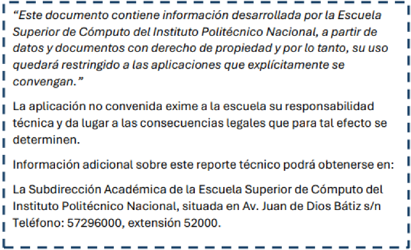
\includegraphics[width=0.75\textwidth]{images/advertencia.png}
	\end{center}
	
	\vspace*{\fill}
	
	
	% =========================
	% RESUMEN
	% =========================
	\cleardoublepage
	\thispagestyle{empty}
	
	\newpage
	
	% =========================
	% CARTA de autorizacion
	% =========================
	\cleardoublepage
	\thispagestyle{empty}
	
	%\begin{center}
	%	\includegraphics[
	%	width=\textwidth,
	%	height=\textheight,
	%	keepaspectratio
	%	]{images/cartaA1.jpg}
	%\end{center}
	
	\cleardoublepage

		\cleardoublepage
	\thispagestyle{empty}
	
	%\begin{center}
	%	\includegraphics[
	%	width=\textwidth,
	%	height=\textheight,
	%	keepaspectratio
	%	]{images/cartaA2.jpg}
	%\end{center}
	
	\cleardoublepage
	

	\newpage
	

\cleardoublepage

%% Indice general, de figuras y de tablas
	% Numeración romana para preliminares
	
	% (\frontmatter: numeracion romana y capitulos sin numero)
	\frontmatter

	\tableofcontents

	\listoffigures

	\listoftables

	% Numeración arábiga para el contenido (\mainmatter empieza en pagina derecha)
	\mainmatter
	
	



% =========================
% CONTENIDO
% =========================
%% Introduccion (sin numero de capitulo)
\chapter*{Introducción}
\addcontentsline{toc}{chapter}{Introducción}
\markboth{Introducción}{}

El presente documento expone los avances del Trabajo Terminal 2026-B009, desarrollado en colaboración con la Defensoría de los Derechos Politécnicos (DDP) del Instituto Politécnico Nacional (IPN), cuyo propósito es diseñar e implementar una plataforma web que contribuya a optimizar los procesos de recepción, atención y seguimiento de quejas. Para ello, se analizan las necesidades operativas de la institución, las limitaciones de los procedimientos actuales y las alternativas tecnológicas que pueden contribuir a su mejora. La propuesta contempla la integración de herramientas de inteligencia artificial orientadas a la recuperación de antecedentes, la identificación de posibles duplicidades y la generación de resúmenes narrativos, como mecanismos de apoyo para las actividades del personal de la Defensoría.

El Instituto Politécnico Nacional (IPN) es una institución pública de educación media superior y superior que ofrece programas académicos en distintas áreas del conocimiento. Su organización, funcionamiento y atribuciones se encuentran regulados por disposiciones institucionales específicas que establecen su estructura y las funciones de sus órganos internos \cite{ipn_ley_organica}. En este marco institucional se encuentra la Defensoría de los Derechos Politécnicos, órgano encargado de promover, proteger y defender los derechos de la comunidad politécnica.

La Defensoría de los Derechos Politécnicos desempeña sus funciones dentro de la estructura institucional del IPN, de acuerdo con las atribuciones establecidas en su marco normativo \cite{ipn_acuerdo622, ipn_manual_organizacion_ddp}. Su actuación comprende actividades relacionadas con la orientación, recepción y atención de asuntos que involucran posibles vulneraciones de derechos. Si bien la DDP cuenta con atribuciones y funciones propias para el cumplimiento de sus responsabilidades, estas se desarrollan dentro del marco jurídico e institucional del IPN. El cumplimiento de dichas funciones requiere procedimientos que permitan administrar la información de manera organizada y dar seguimiento a las quejas presentadas por la comunidad politécnica.

Los procedimientos de atención de quejas de la DDP presentan áreas de oportunidad relacionadas con la digitalización y la organización de sus actividades internas. De acuerdo con el análisis de sus procesos y la documentación institucional, determinadas actividades de recepción, revisión y seguimiento requieren la intervención directa del personal responsable \cite{ipn_manual_procedimientos_ddp}. Esta dependencia puede incrementar la carga administrativa, dificultar la consulta de información y limitar la automatización de tareas repetitivas.

Asimismo, la revisión de las quejas requiere analizar los hechos descritos por los quejosos, consultar expedientes anteriores e identificar posibles coincidencias con casos previamente registrados. Estas actividades pueden demandar tiempo cuando la información se encuentra distribuida en distintos registros o cuando las descripciones presentan diferencias en su redacción. Por ello, resulta pertinente incorporar mecanismos tecnológicos que faciliten la recuperación de antecedentes, la identificación de posibles duplicidades y el énfasis en el contenido relevante de las quejas, además de apoyar la gestión y consulta de los expedientes.

La transformación digital ofrece alternativas para mejorar la administración de información y la ejecución de procesos institucionales. En el ámbito de la atención de quejas, las plataformas informáticas permiten centralizar registros, establecer mecanismos de seguimiento y controlar el acceso a información sensible. Sin embargo, la incorporación de tecnología no debe limitarse a sustituir documentos físicos por formularios electrónicos, sino que debe responder a las necesidades de los usuarios y a las características de los procedimientos existentes. Por esta razón, el desarrollo de una solución para la DDP requiere considerar tanto la gestión administrativa de los casos como las actividades de análisis que intervienen durante su atención.

A partir de las necesidades identificadas, el Trabajo Terminal propone el desarrollo de una plataforma web para administrar el proceso de atención de quejas dentro de la Defensoría. La solución contempla funcionalidades para el registro de quejas, la gestión de expedientes, el seguimiento de casos y la administración de usuarios conforme a sus responsabilidades institucionales. También considera la incorporación de herramientas que apoyen determinadas actividades de análisis y consulta de información. De esta manera, la plataforma busca integrar en un mismo entorno los componentes necesarios para facilitar la operación del personal y mantener organizada la información generada durante las distintas etapas de atención.

Uno de los componentes de inteligencia artificial del proyecto está orientado a la detección de posibles duplicidades y la recuperación de antecedentes mediante técnicas de Procesamiento de Lenguaje Natural (PLN). Este modelo analiza la similitud semántica entre una nueva queja y los expedientes previamente registrados, con el propósito de recuperar antecedentes relacionados e identificar posibles duplicidades que requieran una revisión posterior. Para ello, se emplean técnicas de representación vectorial de textos y recuperación de información que permiten comparar las descripciones de los hechos, incluso cuando se utilizan expresiones diferentes. Los resultados proporcionan al personal de la Defensoría una referencia para localizar antecedentes y reconocer posibles quejas duplicadas, sin sustituir la revisión necesaria para determinar si corresponden a un mismo caso.

El segundo componente de inteligencia artificial se enfoca en la generación automática de resúmenes narrativos a partir de las quejas presentadas por los integrantes de la comunidad politécnica. Su finalidad es transformar descripciones extensas, informales o poco estructuradas en textos concisos y coherentes que conserven los acontecimientos relevantes del relato original. Para ello, se consideran modelos de lenguaje capaces de procesar información textual y generar síntesis en lenguaje natural, estableciendo como criterios de evaluación la fidelidad al contenido original, la conservación de los hechos relevantes y la ausencia de información no sustentada en el relato del quejoso. Este componente busca facilitar la lectura de las quejas y enfatizar sus hechos principales, así como apoyar al personal responsable durante la revisión y documentación de los casos.

La plataforma contempla una arquitectura basada en microservicios para organizar sus funcionalidades en componentes independientes. Este enfoque permite separar responsabilidades, facilitar el mantenimiento y desarrollar modificaciones en determinados módulos sin intervenir directamente en la totalidad del sistema \cite{aws_microservicios, villamizar_microservices}. Entre los componentes considerados se encuentran el portal del quejoso, los módulos administrativos, la gestión de expedientes, los mecanismos de autenticación y autorización, y los servicios relacionados con el procesamiento de información mediante inteligencia artificial. La comunicación entre estos componentes requiere definir interfaces, reglas de acceso y mecanismos de intercambio de datos que permitan mantener la integridad y disponibilidad de la información.

El desarrollo del proyecto se apoya en el levantamiento y análisis de requerimientos realizado en colaboración con personal de la Defensoría. Mediante reuniones de trabajo y revisión de procedimientos institucionales, se identificaron actividades, responsabilidades y reglas de negocio relacionadas con la atención de quejas. Esta información permitió representar procesos mediante diagramas BPMN, elaborar propuestas de interfaces y diseñar estructuras de datos acordes con las necesidades identificadas. Asimismo, se realizaron actividades de implementación de componentes de backend y frontend, junto con pruebas funcionales y experimentales orientadas a revisar el comportamiento de las soluciones desarrolladas. Estos trabajos constituyen la base para continuar con la integración y validación de la plataforma.

La integración de herramientas digitales y de procesamiento de lenguaje natural constituye el enfoque tecnológico propuesto para atender las necesidades identificadas en la DDP. Se espera que la plataforma contribuya a organizar la información, facilitar el seguimiento de expedientes y proporcionar herramientas de apoyo para determinadas actividades administrativas y de análisis. No obstante, el alcance de estos beneficios deberá determinarse mediante las pruebas y evaluaciones correspondientes. En los capítulos siguientes se presentan los antecedentes, fundamentos teóricos, requerimientos, decisiones de diseño, actividades de implementación y procedimientos de evaluación que sustentan el desarrollo del Trabajo Terminal.

%% Capitulo 1. Analisis del problema
\chapter{Análisis del problema}
\label{cap:analisis_problema}
En este capítulo se presenta la problemática que da origen al Trabajo Terminal. En primer lugar, se describe el problema general: la ineficiencia del procedimiento de atención de quejas de la Defensoría de los Derechos Politécnicos. Posteriormente, se desglosa en los problemas específicos que lo conforman y se analizan las causas que los originan. Finalmente, se presenta la propuesta de solución que responde a cada problema específico; los objetivos, el detalle de la propuesta y los riesgos y supuestos del proyecto se presentan en el Capítulo~\ref{cap:proyecto}.

\section{Dominio}
\label{sec:dominio}
El Trabajo Terminal se ubica en el ámbito de la protección de los derechos de la comunidad del Instituto Politécnico Nacional (IPN), institución pública de educación media superior y superior cuya organización, funcionamiento y atribuciones se encuentran regulados por su marco normativo \cite{ipn_ley_organica}. Dentro de su estructura, la Defensoría de los Derechos Politécnicos (DDP) fue creada mediante el acuerdo publicado en la Gaceta Politécnica número 622, en enero de 2006, como el órgano encargado de promover, proteger y defender los derechos de los integrantes de la comunidad politécnica \cite{ipn_acuerdo622}. Las funciones y responsabilidades de sus áreas se establecen en su Manual de Organización \cite{ipn_manual_organizacion_ddp}, mientras que la forma en que debe atenderse cada asunto se describe en su Manual de Procedimientos \cite{ipn_manual_procedimientos_ddp}.

	La DDP atiende a estudiantes, personal académico, personal de apoyo y demás integrantes de la comunidad politécnica. El instrumento central de su labor es la \emph{queja}: un escrito mediante el cual una persona, denominada \emph{quejoso}, hace del conocimiento de la Defensoría hechos que considera una posible vulneración de sus derechos, atribuidos a una persona o a un área del Instituto, a quien se denomina \emph{persona señalada}. Cada queja admitida da origen a un \emph{expediente}, que concentra la narrativa de los hechos, los datos del quejoso, las evidencias presentadas y los documentos que se generan durante su atención, como oficios, citas, notas de análisis y determinaciones. El expediente es, por tanto, el objeto de información sobre el que trabajan todas las áreas de la Defensoría.

	La atención de una queja sigue un procedimiento institucional en el que intervienen distintas áreas de manera sucesiva \cite{ipn_manual_procedimientos_ddp}:

	\begin{itemize}
		\item \textbf{Recepción.} Recibe la queja, verifica que cumpla los requisitos de admisión y, cuando es procedente, la registra y la turna al área correspondiente; en caso contrario, la rechaza o solicita al quejoso que la corrija o complemente.
		\item \textbf{Primer Contacto.} Analiza los hechos descritos, consulta los antecedentes relacionados, puede citar al quejoso o solicitar la versión de la persona señalada y determina si el asunto es competencia de la Defensoría; cuando no lo es, orienta al quejoso o remite el asunto a la instancia competente.
		\item \textbf{Subdefensoría.} Investiga los asuntos admitidos y da seguimiento con las unidades involucradas mediante solicitudes de información sujetas a plazos: la primera solicitud a una unidad cuenta con un plazo de diez días hábiles y las solicitudes subsecuentes, de cinco días hábiles.
		\item \textbf{Titular de la Defensoría.} Supervisa el conjunto de los casos, participa en las etapas de decisión y resolución de los expedientes y coordina la operación de las áreas.
	\end{itemize}

	El dominio presenta características que condicionan cualquier solución tecnológica. En primer lugar, el procedimiento es secuencial: cada área depende de la información generada por la anterior, por lo que la disponibilidad y la integridad del expediente determinan la continuidad de la atención. En segundo lugar, la información principal de cada caso se expresa en lenguaje natural, ya que las narrativas son redactadas libremente por los quejosos. En tercer lugar, los expedientes contienen datos personales y descripciones de situaciones sensibles, por lo que su consulta debe restringirse al personal autorizado según sus responsabilidades. Finalmente, las determinaciones sobre la competencia, la investigación y la resolución de cada asunto corresponden al criterio jurídico del personal de la Defensoría y no pueden delegarse en un sistema informático; cualquier herramienta de apoyo debe, por tanto, auxiliar al personal sin sustituir sus decisiones.

	\section{Problema general}

	El problema central es que este procedimiento resulta ineficiente para el volumen de quejas que recibe la Defensoría. Su ejecución recae principalmente en actividades manuales y secuenciales: el registro y la consulta de los expedientes, la lectura completa de cada narrativa, la búsqueda de antecedentes y la comunicación del avance entre áreas dependen del tiempo y la intervención directa del personal. En consecuencia, el tiempo de atención de cada caso se incrementa, las quejas se acumulan en las distintas etapas y la información necesaria para darles continuidad no siempre está disponible de manera oportuna para quien la requiere. Las dificultades particulares que conforman esta problemática se describen en el siguiente apartado.

	\section{Problemas específicos}
	A partir del levantamiento de requerimientos realizado con el personal de la Defensoría y del análisis de los procedimientos institucionales, se identificaron los siguientes problemas, que en conjunto explican la ineficiencia del proceso descrito.

	\begin{enumerate}
		\item \label{pe:volumen}\textbf{Volumen de quejas superior a la capacidad de atención:}
		De acuerdo con lo señalado por el personal de la Defensoría, el número de quejas que ingresan supera la capacidad del personal para atenderlas y concluirlas en los plazos institucionales. Como cada etapa del procedimiento depende de actividades manuales, el tiempo invertido en tareas de registro, consulta y actualización reduce el tiempo disponible para el análisis de los casos, lo que provoca la acumulación de expedientes pendientes y el retraso en la respuesta a los quejosos.

		\item \label{pe:narrativas}\textbf{Revisión de narrativas extensas:}
		Las quejas contienen descripciones redactadas libremente por los quejosos, que con frecuencia son extensas, repetitivas o no siguen un orden cronológico. Para continuar con el procedimiento, el personal debe leer cada narrativa completa e identificar por sí mismo los hechos relevantes, lo que consume una parte importante del tiempo de revisión de cada expediente.

		\item \label{pe:antecedentes}\textbf{Búsqueda manual de antecedentes:}
		Durante la revisión de una queja es necesario saber si existen expedientes anteriores relacionados con los mismos hechos, personas o unidades. Esta búsqueda se realiza de forma manual y depende de la memoria del personal o de la revisión de registros previos, lo que resulta lento y poco confiable cuando los casos similares están descritos con palabras distintas.

		\item \label{pe:duplicadas}\textbf{Duplicidad de quejas:}
		De acuerdo con lo señalado por el personal de la Defensoría, existen quejosos que presentan nuevamente una solicitud sobre hechos ya reportados, particularmente cuando consideran que no han recibido respuesta. Al no contar con un mecanismo para identificarlas, estas quejas pueden registrarse y atenderse como casos nuevos, lo que duplica el trabajo y fragmenta la información de un mismo asunto.

		\item \label{pe:estado}\textbf{Falta de seguimiento de la queja:}
		No existe un medio único para conocer en qué etapa se encuentra una queja, qué actuaciones se han realizado y qué plazos están por vencer. Esto dificulta priorizar los casos urgentes y obliga a los quejosos a solicitar información sobre el avance de su queja.

		\item \label{pe:informacion}\textbf{Falta de coordinación entre áreas:}
		Cuando un expediente pasa de un área a otra, la información generada en la etapa anterior ---documentos, oficios, citas y determinaciones--- no siempre se encuentra disponible e integrada para quien continúa el procedimiento. Esto provoca consultas adicionales, retrasos y dificultades de coordinación entre el personal.

	\end{enumerate}

	Estos problemas se manifiestan en distintas etapas del procedimiento, pero mantienen una relación directa con la organización de la información, la continuidad de los expedientes y la carga operativa del personal. Su análisis permite identificar los factores que contribuyen a su aparición, los cuales se desarrollan en el siguiente apartado.

	\section{Causas}
	\label{sec:causas}
	Las problemáticas identificadas en la gestión de quejas de la Defensoría de los Derechos Politécnicos se relacionan con diversos factores administrativos, operativos y tecnológicos que intervienen en el desarrollo de sus procedimientos internos. A partir del análisis de los procesos institucionales y de la información obtenida durante el levantamiento de requerimientos, se reconocen condiciones que pueden contribuir a las dificultades de organización, consulta y seguimiento de los expedientes. Las causas se presentan en el mismo orden que los problemas específicos, indicando en cada una el problema que explica.

	\textbf{Dependencia de actividades manuales (problema~\ref{pe:volumen}).} La dependencia de actividades manuales constituye uno de los factores que contribuyen a las dificultades operativas durante la atención de quejas. Los procedimientos institucionales requieren que el personal realice tareas de registro, revisión, actualización y consulta de información en distintas etapas del proceso \cite{ipn_manual_procedimientos_ddp}. Cuando estas actividades dependen principalmente de la intervención humana y carecen de mecanismos que faciliten su ejecución, el tiempo disponible del personal debe distribuirse entre tareas administrativas y actividades que requieren un análisis más detallado. Esta condición puede limitar la capacidad operativa de las áreas responsables, particularmente cuando deben atender varias solicitudes de manera simultánea.

	\textbf{Características de las narrativas (problema~\ref{pe:narrativas}).} Las características de las narrativas presentadas por los quejosos también influyen en el tiempo necesario para revisar las solicitudes. Debido a que los usuarios describen los acontecimientos desde su propia perspectiva, los escritos pueden variar considerablemente en extensión, estructura, claridad y nivel de detalle. Algunas narraciones incluyen información repetida, antecedentes extensos o acontecimientos que no siguen necesariamente un orden cronológico, lo que exige una lectura cuidadosa para identificar los hechos relevantes. La diversidad de estas características dificulta establecer un tiempo uniforme de revisión y aumenta la atención que debe dedicarse a determinados expedientes.

	\textbf{Falta de mecanismos para relacionar expedientes (problemas~\ref{pe:antecedentes} y~\ref{pe:duplicadas}).} La falta de mecanismos especializados para relacionar la información de diferentes expedientes puede contribuir a las dificultades para identificar antecedentes y posibles registros duplicados. Las solicitudes relacionadas con un mismo asunto no siempre presentan una redacción idéntica, debido a que los quejosos pueden describir nuevamente los acontecimientos utilizando expresiones diferentes o incorporando información adicional. Asimismo, distintos expedientes pueden compartir personas involucradas, circunstancias o características sin corresponder necesariamente al mismo hecho. Estas variaciones hacen que la identificación de relaciones entre registros requiera una comparación cuidadosa de su contenido y contexto, de modo que una queja repetida puede pasar inadvertida y registrarse como un caso nuevo.

	\textbf{Ausencia de un registro centralizado del estado de las quejas (problemas~\ref{pe:estado} y~\ref{pe:duplicadas}).} La Defensoría no cuenta con un registro único en el que se consulte la etapa en la que se encuentra cada queja, las actuaciones realizadas y los plazos que están por vencer. Sin esta información, el personal no puede identificar con facilidad los casos detenidos o próximos a vencer ni priorizar su atención, y la supervisión del conjunto de los casos depende de consultas individuales. Del lado del quejoso, la falta de un medio para consultar el avance de su queja provoca que solicite información de manera directa y, cuando considera que no ha recibido respuesta, que presente nuevamente su queja sobre los mismos hechos, lo que da origen a las duplicidades.

	\textbf{Integración limitada de la información entre áreas (problema~\ref{pe:informacion}).} La gestión de una queja involucra documentos, registros y actuaciones generados durante diferentes etapas de atención, en las que intervienen distintos integrantes del personal, cada uno con funciones y responsabilidades específicas conforme a la organización de la Defensoría \cite{ipn_manual_organizacion_ddp}. La continuidad de las actuaciones depende de que la información generada en una etapa se encuentre disponible para quienes participan posteriormente. Cuando la información se administra mediante mecanismos independientes o parcialmente integrados, resulta más complejo conservar una visión completa y actualizada del desarrollo de cada caso, y el traspaso de un expediente entre áreas requiere consultas adicionales que retrasan la atención y dificultan la coordinación de las actividades institucionales.

	\section{Propuesta}
	\label{sec:propuesta}
	Para atender los problemas identificados, se propone una plataforma web para la gestión digital de las quejas de la Defensoría que concentre en un mismo entorno el registro, la atención y el seguimiento de cada expediente, e incorpore dos componentes de inteligencia artificial como apoyo para las actividades de análisis. La plataforma no modifica el procedimiento institucional: lo representa mediante etapas y estados del expediente, de modo que cada área trabaja sobre la misma información y con los permisos que corresponden a su función.

	\begin{itemize}
		\item \textbf{Digitalización del procedimiento (problema~\ref{pe:volumen}).} Se digitaliza el procedimiento completo: el quejoso presenta su queja y sus evidencias desde un portal web y obtiene un folio de seguimiento, mientras que el personal cuenta con un panel para cada área ---Recepción, Primer Contacto, Subdefensoría y Defensora--- desde el cual recibe, valida, turna y atiende los expedientes. Las tareas repetitivas, como el registro, la generación de oficios a partir de plantillas y el envío de notificaciones por correo, se realizan desde la plataforma, lo que reduce el tiempo que el personal dedica a actividades administrativas.

		\item \textbf{Generación de resúmenes (problema~\ref{pe:narrativas}).} Se incorpora un servicio de generación de resúmenes que primero selecciona los fragmentos más relevantes de la narrativa y después los redacta en un texto breve mediante un modelo de lenguaje. El resultado se presenta al personal de Primer Contacto como un borrador que debe revisar y que no sustituye la lectura de la queja original.

		\item \textbf{Búsqueda automatizada de antecedentes (problema~\ref{pe:antecedentes}).} Se incorpora un servicio de búsqueda de antecedentes que, a partir de la narrativa de una queja, recupera los expedientes previos más parecidos combinando una búsqueda por palabras (TF-IDF) con una búsqueda por significado (MiniLM). De esta forma es posible localizar casos relacionados aunque estén redactados con palabras distintas.

		\item \textbf{Detección de posibles duplicidades (problema~\ref{pe:duplicadas}).} El mismo servicio de búsqueda señala las quejas con mayor similitud como posibles duplicidades, para que el personal determine si corresponden al mismo asunto. Además, el quejoso puede consultar el estado de su queja con su folio y su correo, lo que reduce la necesidad de presentarla de nuevo.

		\item \textbf{Seguimiento del estado de la queja (problema~\ref{pe:estado}).} Cada queja tiene un ciclo de vida con estados definidos y un historial de sus actuaciones. El quejoso consulta su avance y recibe avisos en el portal y por correo; la Subdefensoría controla los plazos de las solicitudes de información (diez días hábiles para la primera y cinco para los recordatorios); y la Defensora dispone de un panel de supervisión que señala los casos que requieren atención.

		\item \textbf{Expediente digital único (problema~\ref{pe:informacion}).} Todas las áreas trabajan sobre un expediente único almacenado en una base de datos compartida, que integra documentos, oficios, citas, notas y determinaciones. Al cambiar de etapa, el expediente se turna automáticamente al área siguiente con toda su información, y el acceso a cada operación se controla según el rol del usuario.
	\end{itemize}

	Los componentes de inteligencia artificial funcionan exclusivamente como herramientas de apoyo: sus resultados son revisados por el personal y las decisiones sobre la competencia, la investigación y la resolución de cada asunto permanecen a cargo de la Defensoría. Los objetivos, los componentes y los requerimientos de la propuesta se detallan en el Capítulo~\ref{cap:proyecto}, y su construcción en el Capítulo~\ref{cap:trabajo_realizado}.


%% Capitulo 2. Marco teorico (estado del arte y fundamentos)
\chapter{Marco teórico}

El presente capítulo reúne los antecedentes comparativos y los fundamentos conceptuales que sustentan el Trabajo Terminal. En primer lugar, se recupera el estado del arte desarrollado en Trabajo Terminal I (TT-I), con el propósito de contextualizar la propuesta de la Defensoría de los Derechos Politécnicos (DDP) frente a otras plataformas de recepción y seguimiento de denuncias y quejas. Posteriormente, se presentan los conceptos de Procesamiento de Lenguaje Natural (PLN) necesarios para comprender dos componentes del sistema: la búsqueda de antecedentes y la generación automática de resúmenes.

En los apartados teóricos se explica cada técnica y se precisa su relación con el sistema desarrollado, sin sustituir la descripción de su implementación ni la presentación de resultados experimentales, que corresponden a capítulos posteriores.

\section{Estado del arte de plataformas de denuncia digital}
\label{sec:estado_arte_plataformas}

Durante TT-I se realizó un estudio comparativo de plataformas nacionales e internacionales relacionadas con la recepción, registro y seguimiento de denuncias, quejas y reportes institucionales. La revisión abarcó soluciones gubernamentales, ciudadanas, corporativas y académicas, con el fin de reconocer capacidades de gestión de casos y aspectos relevantes para el contexto de la DDP.

El estudio consideró criterios como seguridad, anonimato, seguimiento, soporte multimedia, automatización, escalabilidad y adaptación al entorno universitario. Estas valoraciones corresponden al análisis documental realizado en TT-I: no son resultados de pruebas técnicas ejecutadas sobre todas las plataformas ni constituyen mediciones comparables de desempeño. Por esa razón, las categorías cualitativas de la tabla deben leerse como apreciaciones del estudio original y no como certificaciones de cada atributo.

\subsection{Comparativa de plataformas}

Se consideraron, entre otras, el Sistema Integral de Denuncias Ciudadanas (SIDEC) \cite{sfp_sidec}, Denuncia Digital de la Ciudad de México \cite{cdmx_denuncia_digital}, MP Virtual \cite{fgjcdmx_mp_virtual}, el Sistema de Atención Mexiquense (SAM) \cite{secogem_sam}, Whistlelink \cite{whistlelink}, EQS Integrity Line \cite{eqs_integrity_line}, NAVEX/WhistleB \cite{navex_whistleb}, Whistleblower Software \cite{whistleblower_software}, BullyButton \cite{bully_button}, Ventanilla Escolar \cite{sep_ventanilla_escolar}, Alerta IPN \cite{ipn_alerta} y Denuncia en Línea de la UNAM \cite{unam_ddu_denuncia}. El análisis de TT-I también incluyó Incorruptible, cuya valoración se conserva para respetar la comparativa original; esta entrada requiere recuperar su fuente documental específica si se pretende utilizar como evidencia independiente.

La Tabla~\ref{tab:comparativa_plataformas} sintetiza las valoraciones registradas en TT-I. Se mantienen las categorías del análisis original para conservar la trazabilidad del estudio; su significado y criterios de asignación deben consultarse junto con la metodología utilizada en esa etapa.

\rowcolors{2}{rowblue}{white}
\footnotesize
\renewcommand{\arraystretch}{1.2}
\setlength{\tabcolsep}{3pt}
\begin{longtable}{|L{2.9cm}|L{1.6cm}|L{1.7cm}|L{1.75cm}|L{1.6cm}|L{1.9cm}|L{1.75cm}|L{1.75cm}|}
\hiderowcolors\caption{Comparativa general de plataformas de denuncia digital}\label{tab:comparativa_plataformas} \\ \showrowcolors
\hline
\rowcolor{headerblue}
\headercell{Plataforma} & \headercell{Seguridad} & \headercell{Anonimato} & \headercell{Seguimiento} & \headercell{Multimedia} & \headercell{Automatización} & \headercell{Escalabilidad} & \headercell{Adaptación universitaria} \\
\hline
\endfirsthead
\hline
\rowcolor{headerblue}
\headercell{Plataforma} & \headercell{Seguridad} & \headercell{Anonimato} & \headercell{Seguimiento} & \headercell{Multimedia} & \headercell{Automatización} & \headercell{Escalabilidad} & \headercell{Adaptación universitaria} \\
\hline
\endhead
SIDEC & Media & Baja & Media & Sí & Baja & Media & No \\ \hline
Denuncia Digital CDMX & Media & Baja & Media & Sí & Baja & Media & No \\ \hline
MP Virtual & Media & Media & Media & Sí & Baja & Media & No \\ \hline
Incorruptible & Baja & Media & Baja & Sí & Baja & Alta & No \\ \hline
SAM & Media & Baja & Media & Sí & Baja & Media & No \\ \hline
Whistlelink & Alta & Alta & Alta & Sí & Media & Alta & Parcial \\ \hline
EQS Integrity Line & Alta & Alta & Alta & Sí & Alta & Alta & Parcial \\ \hline
NAVEX / WhistleB & Alta & Alta & Alta & Sí & Alta & Alta & Parcial \\ \hline
Whistleblower Software & Muy alta & Muy alta & Alta & Sí & Alta & Alta & Parcial \\ \hline
BullyButton & Media & Media & Baja & Limitado & Baja & Media & Sí \\ \hline
Ventanilla Escolar & Media & Baja & Baja & No & Baja & Media & Sí \\ \hline
Alerta IPN & Media & Baja & Media & Sí & Baja & Media & Sí \\ \hline
UNAM Denuncia en Línea & Media & Media & Alta & Sí & Media & Media & Sí \\ \hline
\end{longtable}
\normalsize
\setlength{\tabcolsep}{6pt}
\renewcommand{\arraystretch}{1}

\subsection{Brechas identificadas y relación con la propuesta}

El análisis de TT-I permitió observar diferencias entre las soluciones consideradas. Algunas se orientan a canales generales de denuncia, otras a la protección de informantes y otras a servicios institucionales o educativos. En consecuencia, sus mecanismos de seguimiento, manejo de archivos y adecuación a procedimientos universitarios no responden necesariamente a las mismas necesidades.

Para la DDP, la revisión sirvió como referencia al delimitar funciones como la organización de expedientes, el seguimiento de quejas, el acceso según las responsabilidades del personal y el apoyo a la consulta documental. Asimismo, el estudio motivó la exploración de componentes de PLN para recuperar antecedentes potencialmente relacionados y elaborar resúmenes de apoyo a la revisión de casos. Estas decisiones se fundamentan teóricamente en las siguientes secciones.

Las diferencias señaladas no permiten concluir, por sí solas, que una plataforma específica carezca de una capacidad que no fue documentada en las fuentes consultadas. Del mismo modo, los atributos identificados en TT-I no deben confundirse con los atributos implementados o medidos en el sistema desarrollado; estos últimos se describen y evalúan en los capítulos correspondientes.

\section{Procesamiento de Lenguaje Natural}
\label{sec:fundamentos_pln}

El Procesamiento de Lenguaje Natural (PLN) es una rama de la inteligencia artificial que estudia métodos para analizar, interpretar y generar información expresada en lenguaje humano \cite{jurafsky2023slp}. Entre sus aplicaciones se encuentran la recuperación de información, la comparación documental y la elaboración automática de resúmenes.

El lenguaje presenta variaciones de vocabulario, redacción, extensión y contexto. Dos personas pueden describir acontecimientos semejantes con términos diferentes, mientras que narraciones con palabras coincidentes pueden referirse a hechos distintos. Esta dificultad resulta relevante en las quejas dirigidas a la DDP, pues la información se presenta principalmente como relatos escritos. Para procesarlos, es necesario convertir el texto en unidades y representaciones que puedan analizarse computacionalmente.

\subsection{Preprocesamiento de textos}

El preprocesamiento consiste en preparar el contenido textual para su análisis mediante técnicas computacionales. Su propósito es identificar las unidades lingüísticas relevantes y, cuando resulta necesario, reducir variaciones que puedan dificultar la comparación entre documentos. En la representación léxica son especialmente relevantes la tokenización, la identificación de secuencias de términos y el tratamiento de palabras frecuentes \cite{jurafsky2023slp}. No todas las transformaciones lingüísticas son apropiadas para todas las representaciones: el procesamiento de TF-IDF debe distinguirse de la tokenización interna del modelo semántico.

\paragraph{Tokenización.}

La tokenización divide un texto en unidades denominadas \textit{tokens}, que pueden corresponder a palabras, signos de puntuación u otros elementos lingüísticos. Esta operación permite identificar los componentes de una oración para su posterior análisis. En la búsqueda de antecedentes, la identificación de unidades textuales es relevante para construir las características léxicas utilizadas por TF-IDF; debe distinguirse de la tokenización propia del modelo MiniLM, que utiliza su vocabulario y reglas de codificación.

Por ejemplo, la expresión ``El profesor negó el acceso'' puede dividirse en los siguientes tokens:

\begin{center}
    [\texttt{El}, \texttt{profesor}, \texttt{negó},
    \texttt{el}, \texttt{acceso}]
\end{center}

\paragraph{Unigramas y bigramas.}

Un unigrama representa un término individual, mientras que un bigrama conserva una secuencia de dos términos consecutivos. Considerar ambas unidades permite recoger coincidencias de vocabulario y expresiones cortas cuyo significado depende de la combinación de palabras. En el componente de antecedentes se utiliza TF-IDF con unigramas y bigramas. Esta decisión es relevante para expresiones como ``no autorizó'', en las que considerar únicamente términos aislados puede perder información sobre la relación entre palabras.

\paragraph{Tratamiento de palabras vacías.}

Las palabras vacías, conocidas como \textit{stop words}, son términos frecuentes que, dependiendo de la tarea, pueden aportar poca información para distinguir documentos. Entre ellas se encuentran determinados artículos, preposiciones y conjunciones.

Sin embargo, su eliminación debe realizarse cuidadosamente, ya que expresiones como ``no'', ``sin'' y ``nunca'' pueden modificar el significado de los acontecimientos descritos en una queja. Por esta razón, el preprocesamiento debe considerar las características del contenido y los requisitos del modelo utilizado.

En las narrativas de las quejas, conservar las negaciones es importante para no alterar los hechos descritos. Por ello, al construir representaciones léxicas deben valorarse las consecuencias de eliminar términos frecuentes. Este tratamiento no debe confundirse con la tokenización interna de MiniLM, que sigue las reglas del codificador empleado.

\subsection{Representación vectorial del texto}

La representación vectorial transforma textos en estructuras numéricas que permiten realizar operaciones de comparación y recuperación de información \cite{manning2008ir}. Cada vector describe ciertas propiedades del documento: en una representación léxica, sus dimensiones pueden corresponder a términos o secuencias de términos; en una representación semántica, recogen características aprendidas por un modelo a partir del contexto lingüístico.

Estas dos clases de representación no son equivalentes. La primera facilita la identificación de coincidencias explícitas de vocabulario, mientras que la segunda ayuda a comparar expresiones diferentes que pueden tener significados relacionados. En la búsqueda de antecedentes del sistema se emplean ambas: TF-IDF proporciona la representación léxica y MiniLM genera la representación semántica. Los fundamentos particulares de cada método se explican en la sección dedicada a la recuperación de información.

\section{Recuperación de información y búsqueda de antecedentes}
\label{sec:busqueda_antecedentes}

La búsqueda de antecedentes consiste en localizar documentos previamente registrados que mantienen alguna relación con una nueva solicitud. En la gestión de quejas, esta actividad permite consultar expedientes que presentan semejanzas en los hechos descritos, las circunstancias o las personas involucradas. Su propósito es facilitar el acceso a información relevante para la revisión de los casos, sin establecer automáticamente que los documentos recuperados corresponden a una misma situación.

La identificación de posibles duplicidades constituye una tarea relacionada, pero distinta de la recuperación de antecedentes. Mientras que la primera busca reconocer solicitudes que podrían referirse a hechos previamente reportados, la segunda permite localizar documentos relacionados, aunque correspondan a acontecimientos diferentes. Ambas tareas requieren mecanismos de recuperación y comparación de información textual.

\subsection{Recuperación de información textual}

La recuperación de información es el proceso mediante el cual se identifican documentos relevantes dentro de una colección a partir de una consulta. Su funcionamiento comprende la organización de los documentos disponibles, el procesamiento de la consulta y la aplicación de criterios que permitan determinar cuáles registros presentan mayor relación con la información solicitada \cite{manning2008ir}.

En los sistemas de recuperación textual, los documentos pueden representarse mediante estructuras que facilitan su búsqueda. A partir de sus representaciones se calculan medidas de relevancia para ordenar los resultados y presentar primero aquellos que mantienen una mayor relación con la consulta. En el componente desarrollado, esta comparación se apoya en señales léxicas y semánticas que se explican en los apartados siguientes.

En el contexto de la DDP, una queja puede utilizarse como consulta para recuperar expedientes previamente registrados. De esta manera, el proceso de recuperación permite identificar antecedentes potencialmente relacionados con los hechos descritos y proporciona referencias documentales para su posterior revisión.

\subsection{Representación léxica mediante TF-IDF}

Como antecedente de los métodos de ponderación léxica, el modelo de bolsa de palabras, conocido como \textit{Bag of Words} (BoW), representa un documento mediante la frecuencia de aparición de sus términos, sin considerar el orden en el que se presentan. Aunque permite comparar documentos a partir de su vocabulario, no representa directamente las relaciones de significado entre las palabras \cite{manning2008ir}.

TF-IDF (\textit{Term Frequency--Inverse Document Frequency}) es un método de ponderación que, a partir de los términos presentes en los documentos, asigna un peso según su frecuencia en cada texto y su distribución en la colección.

Su expresión general es:

\begin{equation}
    \operatorname{tf-idf}(t,d,D)
    =
    \operatorname{tf}(t,d)
    \times
    \operatorname{idf}(t,D)
    \label{eq:tfidf}
\end{equation}

donde $t$ representa un término, $d$ un documento y $D$ el conjunto de documentos. El componente TF mide la frecuencia del término dentro del documento, mientras que IDF reduce la importancia de los términos que aparecen en numerosos documentos \cite{manning2008ir}.

En el componente de búsqueda de antecedentes, TF-IDF se aplica sobre unigramas y bigramas de las narrativas para representar las quejas y obtener una señal de coincidencia léxica. Esta señal ayuda a recuperar expedientes que comparten vocabulario y expresiones relevantes. No obstante, dos relatos sobre situaciones semejantes pueden emplear palabras distintas; por ello, el sistema complementa este enfoque con representaciones semánticas generadas mediante MiniLM.

\subsection{Representación semántica mediante Transformers y MiniLM}

Los \textit{embeddings} contextuales generan representaciones que consideran las relaciones entre las palabras de una secuencia. Estos enfoques permiten incorporar información del contexto y representar oraciones o documentos mediante vectores que reflejan características de su contenido semántico.

En los sistemas de recuperación semántica, estos vectores permiten comparar consultas y documentos con una medida de proximidad, incluso cuando no comparten exactamente las mismas palabras. Los modelos utilizados para obtener estas representaciones se describen a continuación.

En la búsqueda de antecedentes, estas representaciones permiten comparar narrativas que expresan hechos relacionados mediante vocabulario distinto. Por ejemplo, dos relatos pueden referirse a una restricción para presentar un examen sin utilizar exactamente los mismos términos. Esta capacidad complementa la coincidencia léxica, aunque la proximidad de los vectores no demuestra por sí sola que los expedientes describan un mismo acontecimiento.

La arquitectura \textit{Transformer} utiliza mecanismos de atención para modelar relaciones entre elementos de una secuencia \cite{vaswani2017attention}. Algunas de sus variantes se emplean como codificadores
(\textit{encoders}) para transformar secuencias de texto en representaciones numéricas. A diferencia
de los métodos que representan los documentos únicamente a partir de la frecuencia de sus términos, estos modelos incorporan relaciones contextuales aprendidas durante su entrenamiento.

El enfoque \textit{Sentence-BERT} (SBERT) adapta modelos Transformer para producir
\textit{embeddings} de oraciones comparables mediante medidas como la similitud coseno. Su empleo
en recuperación semántica permite obtener representaciones de consultas y documentos para identificar cercanía de significado sin comparar cada par de textos con un modelo de clasificación
\cite{reimers2019sbert}.

MiniLM es una familia de modelos Transformer compactos obtenidos mediante técnicas de destilación de conocimiento, orientadas a conservar parte de la capacidad de representación de modelos más grandes con menor costo de inferencia \cite{wang2020minilm}. En el sistema se utiliza la variante multilingüe \texttt{paraphrase-multilingual-MiniLM-L12-v2}, distribuida mediante Sentence Transformers \cite{hf_minilm_multilingual}, para generar las representaciones semánticas de las quejas. Esta variante permite obtener vectores comparables de textos en español y aporta una señal semántica complementaria a las coincidencias de términos identificadas mediante TF-IDF.

Es importante distinguir los codificadores de los modelos generativos: los primeros se utilizan aquí para obtener representaciones vectoriales y comparar textos, mientras que los segundos producen nuevas secuencias de lenguaje. La cercanía entre \textit{embeddings} no demuestra por sí sola que dos expedientes describan los mismos hechos.

\subsection{Similitud coseno}

La similitud coseno es una medida matemática utilizada para comparar la orientación de dos vectores en un espacio multidimensional. Se calcula mediante el producto punto de ambos vectores dividido entre el producto de sus normas, lo que permite estimar su proximidad angular independientemente de sus magnitudes \cite{manning2008ir}.

Para dos vectores no nulos $\mathbf{u}$ y $\mathbf{v}$, la similitud coseno se define como:

\begin{equation}
    \operatorname{sim}(\mathbf{u},\mathbf{v})
    =
    \frac{\mathbf{u}\cdot\mathbf{v}}
    {\lVert\mathbf{u}\rVert\lVert\mathbf{v}\rVert}
    =
    \frac{\displaystyle\sum_{i=1}^{d}u_i v_i}
    {\sqrt{\displaystyle\sum_{i=1}^{d}u_i^2}
     \sqrt{\displaystyle\sum_{i=1}^{d}v_i^2}}
    \label{eq:similitud_coseno}
\end{equation}

donde $d$ representa el número de dimensiones de los vectores. Su resultado se encuentra en el intervalo $[-1,1]$, y los valores cercanos a $1$ indican una mayor proximidad en la dirección de las representaciones.

En la comparación de documentos, esta medida permite ordenar los textos de acuerdo con su similitud vectorial. En el componente de antecedentes se emplea para comparar las representaciones de las quejas y contribuir al ordenamiento de los documentos recuperados. Su interpretación depende del tipo de vector comparado: una coincidencia léxica ponderada por TF-IDF no equivale a una relación semántica obtenida a partir de MiniLM.

No obstante, la similitud coseno mide proximidad entre representaciones y no verifica por sí misma la identidad de los hechos descritos. Por tanto, su utilización en la búsqueda de antecedentes permite identificar coincidencias relevantes, pero no constituye una confirmación automática de duplicidad.

\subsection{Recuperación híbrida de antecedentes}

La recuperación híbrida combina señales provenientes de métodos distintos con la finalidad de aprovechar sus capacidades complementarias. En el sistema propuesto se integran una señal léxica, obtenida mediante TF-IDF, y una señal semántica, calculada a partir de las representaciones generadas con MiniLM. La primera permite recuperar coincidencias de términos y expresiones específicas; la segunda facilita la identificación de textos relacionados incluso cuando están redactados con un vocabulario diferente.

La integración de ambas señales requiere una regla de combinación que establezca la contribución relativa de cada enfoque. Combinar directamente las puntuaciones presenta una dificultad: la similitud obtenida con TF-IDF y la obtenida con MiniLM se expresan en escalas distintas, por lo que sus valores no son comparables. Una alternativa es la fusión por rango recíproco, conocida como \textit{Reciprocal Rank Fusion} (RRF), que combina las posiciones que cada recuperador asigna a un documento en lugar de sus puntuaciones \cite{cormack2009rrf}. En su variante ponderada, la puntuación de un documento $d$ se calcula como:

\begin{equation}
    \operatorname{RRF}(d) = \sum_{r \in \mathcal{R}} \frac{w_r}{c + \operatorname{rango}_r(d)},
    \label{eq:rrf}
\end{equation}

donde $\mathcal{R}$ es el conjunto de recuperadores, $w_r$ el peso asignado al recuperador $r$, $\operatorname{rango}_r(d)$ la posición del documento en la lista de ese recuperador y $c$ una constante de suavizado que reduce la diferencia entre las primeras posiciones. Los documentos que aparecen en posiciones altas en ambas listas obtienen las puntuaciones más elevadas. En el recuperador desarrollado se emplea esta fusión ponderada para combinar las listas de TF-IDF y MiniLM; los valores concretos de las ponderaciones y sus resultados se presentan en los capítulos de pruebas y resultados.

El valor de relevancia producido por la recuperación híbrida permite ordenar antecedentes potenciales, pero no representa por sí mismo una probabilidad de que dos quejas describan los mismos hechos ni determina automáticamente que exista duplicidad. La decisión final corresponde a la revisión de los expedientes.

\subsection{Identificación de posibles duplicidades}

La identificación de documentos relacionados consiste en analizar los resultados de recuperación para reconocer registros que comparten información relevante con una consulta. Esta relación puede establecerse mediante semejanzas en las narrativas, coincidencias de términos específicos o características comunes de los acontecimientos descritos.

En la gestión de quejas, los documentos relacionados pueden corresponder a antecedentes de una situación, solicitudes que involucran a una misma persona o registros que describen acontecimientos semejantes. Sin embargo, estas relaciones no son equivalentes entre sí, ya que dos expedientes pueden compartir elementos sin referirse necesariamente a los mismos hechos.

La detección de posibles duplicidades requiere una consideración adicional: determinar si diferentes solicitudes podrían corresponder a un acontecimiento previamente registrado. Para ello, la similitud textual constituye un criterio de apoyo, pero no una prueba suficiente, debido a que una misma situación puede describirse de distintas maneras y diferentes acontecimientos pueden presentar narrativas similares.

Por tanto, los resultados de recuperación deben interpretarse como coincidencias potencialmente relevantes que requieren revisión. Esta distinción permite utilizar las técnicas de comparación documental sin atribuirles capacidades de verificación que exceden el análisis del contenido textual.

\subsection{Evaluación de la recuperación de antecedentes}

La evaluación de un sistema de recuperación de información permite determinar qué tan adecuadamente identifica documentos relevantes a partir de una consulta. Para ello, se requiere un conjunto de referencia en el que se conozca qué documentos deben considerarse relevantes, de manera que los resultados obtenidos puedan compararse con las relaciones esperadas \cite{manning2008ir}.

Entre las métricas utilizadas para evaluar sistemas de recuperación se encuentran la precisión y la exhaustividad en los primeros $k$ resultados, representadas mediante
$P_k$ y $R_k$, respectivamente, y denotadas también como P@$k$ y R@$k$.

La precisión en los primeros $k$ resultados se define como:

\begin{equation}
    P_k =
    \frac{\text{Documentos relevantes recuperados en los primeros } k}
    {k}
    \label{eq:precision_k}
\end{equation}

Esta métrica indica qué proporción de los documentos presentados en las primeras posiciones resulta relevante para la consulta.

Por su parte, la exhaustividad en los primeros $k$ resultados se expresa como:

\begin{equation}
    R_k =
    \frac{\text{Documentos relevantes recuperados en los primeros } k}
    {\text{Total de documentos relevantes}}
    \label{eq:recall_k}
\end{equation}

Esta medida permite conocer qué proporción de los documentos relevantes disponibles se encuentra entre los primeros resultados recuperados.

Ambas métricas ofrecen perspectivas complementarias sobre el funcionamiento de un sistema de búsqueda. Mientras que la precisión ($P_k$) permite valorar la pertinencia de los resultados presentados, la exhaustividad o \textit{recall} ($R_k$) permite identificar la capacidad del sistema para recuperar los antecedentes relevantes existentes en la colección.

En las pruebas del componente de antecedentes, estas medidas permiten valorar si las quejas relacionadas aparecen entre los primeros resultados de búsqueda, a partir de relaciones de relevancia definidas para el conjunto de evaluación. La selección de las métricas y los valores de $k$ debe corresponder a los objetivos y condiciones de evaluación establecidos para el modelo.

La comparación de configuraciones del recuperador requiere consultas con relaciones de relevancia previamente establecidas y criterios definidos antes de examinar los resultados. Debe distinguirse entre los datos empleados para ajustar parámetros y aquellos destinados a evaluar el comportamiento final, pues utilizar los mismos casos para ambas actividades puede producir estimaciones optimistas. Cuando varias consultas se derivan de un mismo expediente o escenario, es conveniente mantenerlas en un mismo grupo para reducir la fuga de información.

Las pruebas con quejas sintéticas permiten estudiar el comportamiento del sistema en condiciones controladas, pero sus resultados no equivalen a una validación institucional con expedientes reales. Por ello, las métricas obtenidas deben interpretarse junto con el tamaño y las características del conjunto de prueba, los criterios de relevancia y la configuración evaluada.

\section{Generación automática de resúmenes}
\label{sec:generacion_resumenes}

A diferencia de la recuperación de antecedentes, cuyo propósito es comparar y ordenar documentos, la generación de resúmenes busca producir una versión condensada de su contenido. La generación automática de resúmenes es una tarea del Procesamiento de Lenguaje Natural que consiste en producir una versión más breve de un documento, conservando la información necesaria para comprender su contenido. Su propósito es reducir la extensión del texto sin perder los elementos esenciales que permiten interpretar el mensaje original \cite{jurafsky2023slp}.

Esta tarea resulta especialmente relevante cuando se trabaja con documentos extensos que contienen información narrativa. En estos casos, un resumen permite identificar los acontecimientos principales, las circunstancias descritas y las relaciones entre los hechos, sin necesidad de revisar inicialmente la totalidad del documento.

En el contexto de la DDP, las quejas pueden contener descripciones extensas de acontecimientos, antecedentes y circunstancias particulares. La generación automática de resúmenes puede facilitar una primera revisión del contenido y apoyar la consulta de los expedientes. Sin embargo, el resumen generado no sustituye el documento original ni la valoración realizada por el personal responsable.

\subsection{Resumen extractivo y abstractivo}

Los métodos de generación automática de resúmenes pueden clasificarse principalmente en extractivos y abstractivos, de acuerdo con la manera en que construyen el texto resultante \cite{jurafsky2023slp}.

El resumen extractivo consiste en seleccionar fragmentos del documento original que contienen información considerada relevante. Estos fragmentos, generalmente oraciones completas, se organizan para construir una versión reducida del texto. Su principal característica es que conserva las expresiones utilizadas en el documento de origen.

Por ejemplo, si una queja contiene varias oraciones que describen un acontecimiento, un método extractivo puede seleccionar aquellas que proporcionan mayor información sobre los hechos, omitiendo detalles repetitivos o secundarios.

Por su parte, el resumen abstractivo genera una nueva redacción a partir de la información identificada en el documento. A diferencia del enfoque extractivo, no se limita a copiar fragmentos, sino que puede reformular oraciones, integrar información relacionada y producir expresiones que no aparecen literalmente en el texto original.

Esta capacidad permite construir resúmenes narrativos más cohesionados. No obstante, también introduce el riesgo de generar afirmaciones que no se encuentran respaldadas por el documento de origen.

Para la gestión de quejas, esta distinción resulta importante debido a que la claridad del resumen debe mantenerse subordinada a la conservación de los hechos descritos por la persona que presenta la solicitud.

\subsection{Selección de fragmentos mediante Maximum Marginal Relevance}

La selección extractiva de oraciones puede producir resúmenes redundantes cuando varios fragmentos expresan información semejante. \textit{Maximum Marginal Relevance} (MMR) es un criterio que busca equilibrar la relevancia de una unidad respecto al documento o consulta y su novedad frente a las unidades ya seleccionadas \cite{carbonell1998mmr}.

Una formulación habitual escoge iterativamente la unidad $s$ que maximiza:

\begin{equation}
    \operatorname{MMR}(s) =
    \lambda\,\operatorname{sim}(s,q) -
    (1-\lambda)\max_{s'\in S}
    \operatorname{sim}(s,s'),
    \label{eq:mmr}
\end{equation}

donde $q$ representa el texto o consulta de referencia, $S$ es el conjunto de unidades seleccionadas y $\lambda\in[0,1]$ regula el equilibrio entre relevancia y redundancia. Para la primera selección, cuando $S$ está vacío, el término de redundancia se considera nulo.

En textos narrativos, MMR proporciona una base para elegir fragmentos informativos sin repetir innecesariamente el mismo contenido. Sin embargo, no garantiza por sí solo la conservación de fechas, negaciones, actores, consecuencias o relaciones cronológicas. Por ese motivo, puede complementarse con reglas de cobertura y coherencia contextual. En el componente de resúmenes de la DDP, MMR se utiliza para seleccionar fragmentos de la queja antes de enviarlos al modelo Qwen3. De esta forma se busca concentrar la entrada en contenido informativo y reducir repeticiones innecesarias. La selección y la redacción posterior son etapas diferentes: MMR decide qué contenido se proporciona al generador, mientras que Qwen3 determina cómo se expresa ese contenido en el resumen.

\subsection{Modelos de lenguaje generativos y Qwen3}

Los modelos de lenguaje son sistemas computacionales diseñados para procesar y generar secuencias de texto mediante el aprendizaje de patrones lingüísticos. Sus aplicaciones incluyen la comprensión de documentos, la generación de respuestas y la elaboración automática de resúmenes \cite{jurafsky2023slp}.

Como se explicó en la recuperación semántica, los Transformers emplean mecanismos de atención para representar las relaciones entre los elementos del texto \cite{vaswani2017attention}. No obstante, los modelos basados en esta arquitectura pueden tener funciones diferentes: MiniLM se utiliza como codificador para producir representaciones comparables, mientras que Qwen3 se emplea como modelo generativo para redactar resúmenes. Esta diferencia permite distinguir la recuperación de información de la producción de nuevas secuencias lingüísticas.

Los modelos de lenguaje basados en Transformers pueden utilizarse para desarrollar sistemas de resumen abstractivo. A partir de un documento de entrada, estos modelos generan una secuencia de texto que busca representar su contenido principal mediante una redacción más breve y organizada.

Sin embargo, la capacidad de generar lenguaje coherente no garantiza que todas las afirmaciones producidas correspondan fielmente al documento original. Por ello, la utilización de estos modelos requiere considerar mecanismos de evaluación y revisión de los resultados.

\paragraph{Generación autorregresiva con Qwen3.}

Para la etapa de redacción del resumen se utiliza el modelo \texttt{Qwen3-4B-Instruct-2507}, perteneciente a la familia Qwen3 \cite{hf_qwen3_4b_instruct_2507}, que trabaja a partir de los fragmentos seleccionados mediante MMR. Los modelos de lenguaje generativos de tipo \textit{decoder} producen texto de manera autorregresiva: predicen el siguiente token condicionado por los anteriores y repiten el procedimiento hasta completar la salida. Aunque el procesamiento de una entrada utiliza operaciones paralelizables, los tokens de salida se generan secuencialmente, de modo que la longitud de la respuesta influye en el tiempo total de inferencia.

En el componente de resúmenes, Qwen3 recibe como material de entrada los fragmentos previamente seleccionados con MMR y produce una redacción condensada. Los modelos generativos pueden recibir instrucciones que establecen el propósito, el estilo y las restricciones del texto generado. En una tarea de redacción institucional, es posible solicitar la transformación de fragmentos a tercera persona y pedir que se conserven negaciones, actores y datos explícitos. No obstante, las instrucciones no constituyen una garantía formal de fidelidad factual, por lo que deben complementarse con evaluación y revisión.

\subsection{Fidelidad y consistencia factual}

La fidelidad factual es una propiedad fundamental de los resúmenes automáticos y se refiere a la correspondencia entre las afirmaciones del resumen y la información contenida en el documento original.

Un resumen puede presentar una redacción clara y gramaticalmente correcta sin representar adecuadamente los acontecimientos descritos. Esto ocurre cuando se incorporan datos inexistentes, se modifican relaciones entre los hechos o se omiten elementos necesarios para comprender una situación.

En los modelos generativos, la producción de información que no está respaldada por el documento de entrada se conoce comúnmente como alucinación. Este fenómeno representa una limitación importante en aplicaciones donde la exactitud del contenido resulta esencial.

En el contexto de las quejas, las alteraciones pueden afectar aspectos como las personas involucradas, las fechas, las acciones atribuidas a cada participante o la secuencia de los acontecimientos. Por ejemplo, modificar quién realizó una acción puede cambiar sustancialmente el significado de la narrativa.

La fidelidad de un resumen requiere, por tanto, preservar las afirmaciones relevantes y evitar incorporar interpretaciones que excedan la información proporcionada. Asimismo, es necesario distinguir entre reducir la extensión del documento y eliminar información que resulta indispensable para comprender los hechos.

Por estas razones, el resumen generado con Qwen3 se presenta en el sistema como un apoyo para la lectura inicial de la queja, no como una sustitución del expediente ni como una interpretación definitiva de los hechos. La revisión por parte del personal responsable sigue siendo necesaria cuando la síntesis se utilice en un proceso institucional.

\subsection{Evaluación de resúmenes automáticos}

La evaluación de resúmenes automáticos busca determinar en qué medida el texto generado conserva la información relevante del documento original y presenta una redacción comprensible.

Entre los aspectos que pueden considerarse se encuentran la cobertura de los hechos principales, la fidelidad factual, la ausencia de información inventada, la coherencia narrativa y la claridad del texto.

Una estrategia de evaluación consiste en comparar el resumen generado con un resumen de referencia elaborado o validado previamente. Esta comparación permite analizar si el sistema recupera los elementos informativos esperados, aunque la existencia de diferentes formas válidas de resumir un documento puede dificultar la evaluación automática.

Por esta razón, las medidas basadas únicamente en coincidencias textuales no son suficientes para determinar la calidad integral de un resumen. Dos textos pueden utilizar expresiones diferentes y conservar los mismos hechos, mientras que una redacción similar puede contener alteraciones importantes en su significado.

En un procedimiento que combina MMR con generación mediante Qwen3, resulta pertinente distinguir dos fuentes de error: la omisión de información durante la selección de fragmentos y la modificación u omisión de hechos durante la generación. Para diferenciarlas se puede examinar, primero, la cobertura factual de los fragmentos seleccionados frente a la queja original y, después, la fidelidad del resumen frente a esos fragmentos y frente al documento completo. Esta evaluación por etapas constituye un criterio metodológico y no debe presentarse como una validación exhaustiva ya realizada. Su aplicación con quejas reales y revisión del personal de la DDP quedó fuera del alcance temporal del proyecto.

La revisión humana complementa la evaluación automática mediante la identificación de errores factuales, omisiones relevantes y problemas de interpretación. En documentos que describen posibles vulneraciones de derechos, esta revisión adquiere especial importancia debido a las consecuencias que puede tener una representación incorrecta de los acontecimientos.

Para la DDP, una evaluación posterior con expedientes reales y criterios acordados con el personal responsable deberá considerar tanto su utilidad para facilitar la lectura de las quejas como su capacidad para conservar la información necesaria para comprender cada caso. El resultado debe interpretarse como una síntesis de apoyo y no como una sustitución del expediente original.

%% Capitulo 3. Proyecto (objetivos, metodologia, alcances, requerimientos)
\chapter{Proyecto}
\label{cap:proyecto}

\section{Objetivos}
\label{sec:objetivos}

\subsection{Objetivo general}
Desarrollar una plataforma web basada en una arquitectura de microservicios mediante la integración de módulos de gestión documental y un motor de procesamiento de lenguaje natural para sistematizar el flujo operativo de recepción, clasificación y seguimiento de quejas de la DDP.

\subsection{Objetivos específicos}
\begin{itemize}
    \item \textbf{Analizar} el marco normativo de la Defensoría de los Derechos Politécnicos y sus manuales de procedimientos para definir las reglas de negocio que permitan la transición de la gestión analógica a un flujo de trabajo digitalizado.

    \item \textbf{Diseñar} la arquitectura del sistema basada en microservicios, asegurando la integridad de los datos y una experiencia de usuario (UX) accesible mediante:
    \begin{itemize}
        \item \textit{Arquitectura:} establecer un diseño modular que soporte la alta demanda de la comunidad politécnica y garantice la seguridad de la información sensible.
        \item \textit{Base de datos:} estructurar un esquema centralizado que elimine la duplicidad de registros y permita la trazabilidad total del expediente.
        \item \textit{UI/UX:} proyectar una interfaz intuitiva para el quejoso y un panel de gestión eficiente para el cuerpo técnico jurídico.
    \end{itemize}

    \item \textbf{Implementar} un módulo mediante técnicas de Procesamiento de Lenguaje Natural (PLN) para asistir en la clasificación preliminar de las quejas y determinar su competencia institucional.

    \item \textbf{Desarrollar} los componentes centrales de la plataforma web, garantizando la operatividad de las siguientes funciones:
    \begin{itemize}
        \item \textit{Gestión de expedientes:} digitalización del ciclo de vida de la queja (recepción, investigación y resolución) para optimizar el tiempo efectivo del personal jurídico.
        \item \textit{Seguimiento:} establecer un sistema de consulta para el quejoso que brinde transparencia sobre el estatus de su trámite.
        \item \textit{Gestión por roles:} implementar controles de acceso estrictos basados en las facultades normativas de cada actor dentro de la Defensoría.
    \end{itemize}
\end{itemize}

\section{Metodología}
\label{sec:metodologia}
Para el desarrollo del Trabajo Terminal se planteó inicialmente una metodología híbrida basada en Scrum-ban, con el fin de organizar en ciclos iterativos las tareas de desarrollo de software, diseño de interfaces y construcción de módulos funcionales. Conforme avanzó el proyecto, este esquema mostró limitaciones que afectaron la continuidad de los ciclos planteados, por lo que se sustituyó por un modelo incremental con prototipado evolutivo. En este apartado se exponen las razones del cambio, el enfoque adoptado y los incrementos en los que se organizó el desarrollo.

\subsection{Justificación del cambio de metodología}
Scrum-ban supone que el equipo cuenta con retroalimentación frecuente del cliente para priorizar, revisar y aceptar el trabajo de cada ciclo. En este proyecto, la Defensoría de los Derechos Politécnicos era la fuente de la retroalimentación operativa, de la validación funcional y de la definición de los requerimientos institucionales. Sin embargo, durante diversas etapas del proyecto existieron periodos prolongados sin disponibilidad para reuniones, revisión de avances o validación de cambios, lo que provocó modificaciones en las prioridades, en los requerimientos y en los tiempos de desarrollo.

Esta situación afectó la estabilidad del tablero Kanban y la planeación de los \textit{sprints}, ya que varias funcionalidades dependían de una validación institucional para darse por terminadas. En consecuencia, los ciclos no podían cerrarse en los tiempos previstos y el tablero dejó de reflejar el avance real del proyecto. Por ello, se determinó que Scrum-ban no representaba adecuadamente la dinámica del proyecto ni la forma en que evolucionaban sus requerimientos.

A lo anterior se suma que el proyecto no se limitó al desarrollo de software: involucró análisis normativo, modelado del procedimiento institucional, diseño arquitectónico, integración de componentes de inteligencia artificial y gestión documental. Estas actividades requieren periodos de investigación cuya duración es difícil de ajustar a ciclos de duración fija.

\subsection{Enfoque metodológico}
Se adoptó un modelo de desarrollo incremental con prototipado evolutivo \cite{pressman2014, sommerville2016}. En el desarrollo incremental, el sistema se construye por partes funcionales que se agregan sucesivamente a una base ya operativa; en el prototipado evolutivo, cada versión se presenta al cliente, se ajusta con sus observaciones y se conserva como base de la siguiente, en lugar de desecharse.

La principal razón de su elección es que permite desacoplar el avance técnico de la disponibilidad inmediata de validación institucional. Cuando la DDP no podía revisar un avance, el equipo continuaba con la arquitectura, el modelo de datos, las interfaces o los componentes de inteligencia artificial del siguiente incremento, y las observaciones recibidas posteriormente se incorporaban como ajustes al prototipo existente. De esta manera fue posible mantener la continuidad del desarrollo aun durante los periodos sin retroalimentación. Además, a diferencia de un enfoque ágil centrado únicamente en ciclos cortos de entrega, este modelo permitió trabajar de forma simultánea en actividades de distinta naturaleza: investigación normativa, diseño de la arquitectura distribuida, modelado de la base de datos, desarrollo del \textit{backend} y del \textit{frontend} e integración de inteligencia artificial.

Cada incremento siguió el mismo ciclo de trabajo:

\begin{enumerate}
    \item \textbf{Análisis:} identificación de las actividades, reglas de negocio y requerimientos del área correspondiente, a partir de los manuales institucionales y de las reuniones con el personal de la Defensoría.
    \item \textbf{Diseño:} definición de los casos de uso, los prototipos de interfaz, los cambios al modelo de datos y los servicios necesarios.
    \item \textbf{Construcción:} desarrollo de los microservicios y de las interfaces web del incremento.
    \item \textbf{Verificación:} pruebas del incremento y de su integración con los componentes ya construidos.
    \item \textbf{Revisión:} presentación del prototipo a la DDP cuando existió disponibilidad, e incorporación de sus observaciones en el mismo incremento o en uno posterior.
\end{enumerate}

\subsection{Incrementos del desarrollo}
El desarrollo se organizó en los siguientes incrementos. Aunque se presentan en orden, varios de ellos se trabajaron de forma parcialmente simultánea, precisamente para aprovechar los periodos sin retroalimentación institucional.

\begin{enumerate}
    \item \textbf{Análisis del procedimiento institucional:} revisión del marco normativo y de los manuales de la Defensoría, reuniones con su personal y elaboración del diagrama BPMN del proceso de atención de quejas.
    \item \textbf{Arquitectura base:} definición de los microservicios, del esquema de la base de datos, del mecanismo de autenticación y del despliegue en contenedores.
    \item \textbf{Portal del quejoso:} presentación de quejas con evidencias, consulta por folio, cuentas de seguimiento y notificaciones.
    \item \textbf{Recepción y administración:} panel de revisión para validar, rechazar y turnar quejas, registro de quejas en papel y consola de administración de cuentas, catálogos, plantillas y respaldos.
    \item \textbf{Primer Contacto y Subdefensoría:} análisis de los expedientes, citas, dictámenes y remisiones, así como la investigación con control de plazos y la elaboración de acuerdos.
    \item \textbf{Componentes de inteligencia artificial:} búsqueda de antecedentes y generación de resúmenes, integrados al módulo de Primer Contacto.
    \item \textbf{Supervisión de la Defensora:} panel de indicadores, seguimiento de las quejas por etapa y por unidad, y carga de trabajo del personal.
    \item \textbf{Pruebas y cierre:} verificación de la plataforma conforme a sus requerimientos funcionales y no funcionales, y corrección de los defectos encontrados.
\end{enumerate}

\section{Propuesta}
\label{sec:propuesta_proyecto}

\subsection{Qué se hará}
El Trabajo Terminal 2026-B009 propone el desarrollo de una plataforma web para la gestión de quejas de la Defensoría de los Derechos Politécnicos (DDP) del Instituto Politécnico Nacional. La plataforma abarcará los procesos de recepción, registro, revisión, atención y seguimiento de quejas mediante la administración de expedientes digitales, de modo que cada área de la Defensoría trabaje sobre la misma información y con los permisos que corresponden a su función.

El desarrollo utilizará una arquitectura basada en microservicios, con aplicaciones web independientes para cada perfil de usuario, e incorporará mecanismos de autenticación, autorización y control de acceso para proteger la información administrada. Como apoyo a la revisión de las quejas, se integrarán dos componentes de inteligencia artificial que funcionarán como herramientas de apoyo para el personal, sin sustituir su criterio ni las decisiones institucionales.

\subsection{Qué incluye la propuesta}
La propuesta contempla los siguientes componentes:

\begin{itemize}
    \item \textbf{Portal del quejoso:} registro de quejas con documentos y evidencias, con o sin cuenta; consulta del estado de la queja mediante folio; notificaciones y respuesta a acuerdos de conciliación.
    \item \textbf{Panel de Recepción:} validación, rechazo y turnado de quejas; registro de quejas recibidas en papel e historial de trámites.
    \item \textbf{Módulo de Primer Contacto:} análisis de expedientes, agenda de citas, oficios, dictamen de competencia y remisión a otras instancias.
    \item \textbf{Módulo de Subdefensoría:} investigación de los expedientes procedentes, solicitudes de información con control de plazos y acuerdos de conciliación y de conclusión.
    \item \textbf{Panel de la Defensora:} supervisión de las quejas y del personal, y administración de cuentas, catálogos, plantillas, respaldos y bitácora.
    \item \textbf{Componentes de inteligencia artificial:} un modelo de búsqueda de antecedentes y detección de posibles duplicidades mediante similitud semántica, y un modelo de generación de resúmenes narrativos que facilite la revisión de las quejas.
\end{itemize}

\subsection{Exclusiones}
La plataforma está orientada a su utilización mediante navegadores web, por lo que no contempla el desarrollo de una aplicación móvil nativa ni la integración con sistemas externos al alcance definido. Tampoco contempla la emisión automatizada de resoluciones o dictámenes jurídicos, ya que estas actividades corresponden exclusivamente al personal autorizado de la Defensoría.

\section{Riesgos y supuestos}
\label{sec:riesgos_supuestos}
\label{sec:limitaciones}
El desarrollo, la implementación y la evaluación del Trabajo Terminal están sujetos a condiciones académicas, tecnológicas e institucionales que pueden influir en el alcance y el funcionamiento de la plataforma. En este apartado se identifican los riesgos del proyecto, con la acción adoptada para mitigar cada uno, y los supuestos sobre los que se planteó la propuesta.

\subsection{Riesgos}

\rowcolors{2}{rowblue}{white}
\small
\renewcommand{\arraystretch}{1.25}
\setlength{\tabcolsep}{4pt}
\begin{longtable}{|L{3.0cm}|L{6.4cm}|L{6.2cm}|}
	\hiderowcolors\caption{Riesgos del proyecto y acciones de mitigación}
	\label{tab:riesgos} \\ \showrowcolors
	\hline
	\rowcolor{headerblue}
	\headercell{Riesgo} & \headercell{Descripción} & \headercell{Mitigación} \\
	\hline
	\endfirsthead
	\hline
	\rowcolor{headerblue}
	\headercell{Riesgo} & \headercell{Descripción} & \headercell{Mitigación} \\
	\hline
	\endhead
	Tiempo de desarrollo & Al tratarse de un proyecto académico con un periodo de ejecución definido, la implementación, integración y validación de los módulos están sujetas al calendario de entregas; algunas funcionalidades podrían quedar incompletas. & Desarrollo incremental que prioriza el flujo principal de atención de quejas y registro explícito del estado de avance de cada componente. \\ \hline
	Disponibilidad de la DDP para validar & Los periodos sin disponibilidad del personal para reuniones o revisiones pueden retrasar la validación de requerimientos y cambios. & Prototipado evolutivo: el desarrollo continúa con otros incrementos y las observaciones se incorporan después al prototipo. \\ \hline
	Disponibilidad de datos & El desarrollo y la evaluación de los modelos de inteligencia artificial dependen de expedientes históricos, cuyo acceso está restringido por tratarse de información sensible. & Uso de conjuntos de datos sintéticos, cuyos resultados se interpretan como preliminares; la validación con expedientes reales queda como trabajo futuro. \\ \hline
	Precisión de los modelos & La búsqueda de antecedentes puede señalar casos que no son duplicidades reales u omitir coincidencias relevantes; el modelo de resúmenes puede presentar omisiones, interpretaciones incorrectas o información no sustentada en el texto original. & Los resultados se presentan como sugerencias o borradores que siempre requieren revisión del personal. \\ \hline
	Infraestructura tecnológica & El funcionamiento de la plataforma y de los modelos depende de la capacidad de procesamiento, memoria y almacenamiento disponible, lo que puede limitar el rendimiento y la ejecución simultánea de servicios. & Los servicios de inteligencia artificial se ejecutan por separado, de modo que su falla o saturación no detiene la operación del resto de la plataforma. \\ \hline
	Protección de datos personales & Los expedientes contienen datos personales y situaciones sensibles cuya exposición tendría consecuencias para las personas involucradas. & Cifrado de las comunicaciones, control de acceso por rol y registro de las acciones administrativas en bitácora. \\ \hline
\end{longtable}
\normalsize
\setlength{\tabcolsep}{6pt}
\renewcommand{\arraystretch}{1}

\subsection{Supuestos}
La propuesta se planteó considerando los siguientes supuestos:

\begin{itemize}
    \item El procedimiento descrito en los manuales de la Defensoría permanece vigente durante el desarrollo, por lo que las reglas de negocio derivadas de ellos siguen siendo válidas.
    \item El personal de la Defensoría participa en reuniones de revisión y validación en los momentos clave del proyecto, aunque no sea de manera continua.
    \item Los usuarios acceden a la plataforma mediante un navegador web actualizado y con conexión a Internet.
    \item Se dispone de servidores para desplegar los contenedores de la plataforma y de un servicio de correo electrónico para el envío de notificaciones.
    \item El tratamiento de expedientes y datos personales se ajusta a las disposiciones institucionales y a la normativa aplicable en materia de protección de datos.
    \item El personal autorizado revisa los resultados de los componentes de inteligencia artificial antes de utilizarlos, ya que estos no sustituyen la revisión, interpretación ni las decisiones jurídicas de la Defensoría.
\end{itemize}


	\section{Actores del sistema}
	\label{sec:actores}
	El análisis distingue a la persona que presenta la queja y a los perfiles institucionales
	que participan en su recepción, análisis, gestión y seguimiento. La organización por roles
	justifica aplicaciones web diferenciadas y políticas de autorización en los servicios: la
	separación de interfaces mejora la adaptación al trabajo de cada área, aunque no sustituye
	la validación de permisos en el servidor.
	
	\begin{itemize}
		\item \textbf{Quejoso.} Cualquier integrante de la comunidad politécnica ---estudiante,
		personal académico o administrativo--- que presenta una queja o le da seguimiento. Es el
		único actor externo y el único que puede operar sin credenciales previas.
	
		\item \textbf{Personal de recepción.} Personal de la Defensoría encargado de recibir,
		validar y canalizar las quejas que llegan por el portal público o en papel.
	
		\item \textbf{Analista de primer contacto.} Consulta expedientes, revisa antecedentes
		relacionados y utiliza borradores de resumen como apoyo al análisis de quejas.
		\item \textbf{Subdefensoría.} Gestiona las actuaciones y el seguimiento que corresponden
		a su área conforme a los permisos asignados.
		\item \textbf{Defensora.} Titular de la Defensoría. Participa en las etapas de decisión y
		resolución del expediente, sin que las herramientas de inteligencia artificial sustituyan sus
		atribuciones; supervisa la operación desde su panel y administra la plataforma: cuentas del
		personal, catálogos, plantillas, respaldos y bitácora de seguridad.
	\end{itemize}
	
	La Tabla~\ref{tab:actores_roles} presenta los perfiles, su rol en el sistema y sus
	responsabilidades generales.

	\rowcolors{2}{rowblue}{white}
	\small
	\renewcommand{\arraystretch}{1.25}
	\setlength{\tabcolsep}{4pt}
	\begin{longtable}{|L{3.8cm}|L{4.8cm}|L{7.0cm}|}
		\hiderowcolors\caption{Actores y roles del sistema}
		\label{tab:actores_roles} \\ \showrowcolors
		\hline
		\rowcolor{headerblue}
		\headercell{Actor} & \headercell{Rol en el sistema} & \headercell{Responsabilidad} \\
		\hline
		\endfirsthead
		\hline
		\rowcolor{headerblue}
		\headercell{Actor} & \headercell{Rol en el sistema} & \headercell{Responsabilidad} \\
		\hline
		\endhead
		Quejoso & ---\ (usuario externo) & Presentar quejas y darles seguimiento \\ \hline
		Personal de recepción & \texttt{RECEPCIONISTA} & Recibir, validar, rechazar y turnar quejas \\ \hline
		Analista de primer contacto & \texttt{ANALISTA\_\allowbreak PRIMER\_\allowbreak CONTACTO} & Análisis de expedientes y consulta de herramientas de inteligencia artificial \\ \hline
		Subdefensor & \texttt{SUBDEFENSOR} & Gestión y seguimiento de actuaciones de su área \\ \hline
		Defensora & \texttt{DEFENSOR} & Supervisión, resolución y cierre del expediente; administración de cuentas, catálogos, plantillas, respaldos y bitácora \\ \hline
	\end{longtable}
	\normalsize
	\setlength{\tabcolsep}{6pt}
	\renewcommand{\arraystretch}{1}

	La Figura~\ref{fig:organigrama} muestra la estructura de la Defensoría y el rol que corresponde a cada área en la plataforma. La Defensoría cuenta con dos subdefensorías ---Atención a los Alumnos y Egresados, y Atención a Personal---, ambas con el rol \texttt{SUBDEFENSOR}.

	\begin{figure}[H]
		\centering
		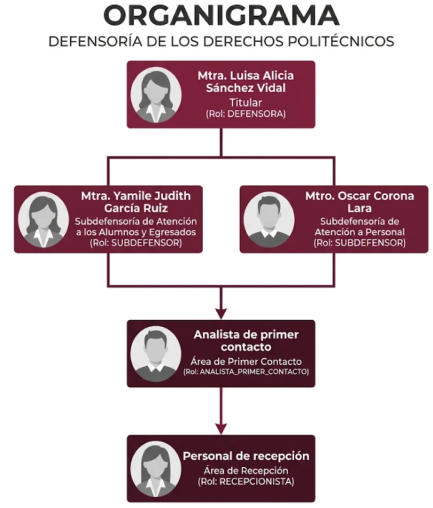
\includegraphics[width=0.6\textwidth]{images/organigrama_ddp.png}
		\caption{Organigrama de la Defensoría de los Derechos Politécnicos y roles en la plataforma}
		\label{fig:organigrama}
	\end{figure}

	Los módulos de Primer Contacto y Subdefensoría forman parte del flujo de trabajo de la
	plataforma. Sus permisos y servicios deben documentarse de manera coherente con la matriz
	de autorización y los casos de uso. Las actividades de resolución corresponden al personal
	institucional autorizado y no se automatizan mediante inteligencia artificial.
	
	\section{Especificación de requerimientos}
	\label{sec:requerimientos}
	El levantamiento de requerimientos combinó la revisión de documentación institucional
	de la Defensoría con reuniones de trabajo para precisar actividades, responsabilidades
	y necesidades de los distintos perfiles. El equipo sostuvo una serie de reuniones con el personal
	de la institución que evolucionaron de forma iterativa: cada sesión aclaró aspectos que la
	anterior había dejado abiertos, y cada avance técnico intermedio se convirtió en insumo de la
	siguiente reunión.
	
	La primera sesión tuvo como objetivo comprender el contexto operativo e identificar las áreas
	que intervienen en la gestión de una queja. Con ese contexto el equipo elaboró un diagrama de
	proceso en notación BPMN a partir de los documentos oficiales, que se presentó en una segunda
	sesión como base de discusión. La revisión permitió aclarar el alcance y la secuencia de distintas actividades,
	incorporar observaciones del personal y ajustar el diagrama para representar el flujo
	de atención acordado para la plataforma. Validado ese diagrama, se establecieron
	sesiones por área para traducir las actividades de cada rol en casos de uso y vistas concretas,
	con sesiones de revisión intermedias para confirmar que los artefactos reflejaran lo acordado.
	
	El resultado acumulado se organizó en tres categorías ---requerimientos funcionales, no
	funcionales y reglas de negocio--- y se estructuró por actor, de modo que cada requerimiento
	tiene un dueño identificable. La nomenclatura empleada codifica el actor en el identificador:
	\texttt{RF-Q} para los requerimientos funcionales del quejoso, \texttt{RF-R} para los del
	personal de recepción, \texttt{RF-PC} para los de Primer Contacto, \texttt{RF-SD} para los de
	Subdefensoría y \texttt{RF-A} para los de la Defensora, y de forma análoga
	\texttt{RNF-} y \texttt{RN-} para los no funcionales y las reglas de negocio. Esta convención permite rastrear cada elemento hasta su origen.
	
	\subsection{Requerimientos funcionales del quejoso}
	Los requerimientos del quejoso se agrupan en cinco bloques: operación sin cuenta, gestión de la
	cuenta, gestión de las quejas propias, seguimiento y servicios de apoyo. El primer bloque es el
	más determinante para el diseño, porque exige que el sistema acepte quejas de personas que no
	tienen ---ni necesariamente quieren tener--- una cuenta, lo que obliga a un punto de acceso
	público sin autenticación y a un mecanismo de identificación posterior basado en el folio.
	
	\small
	\renewcommand{\arraystretch}{1.2}
	\setlength{\tabcolsep}{4pt}
	
	\begin{longtable}{|L{1.7cm}|L{4.0cm}|L{9.9cm}|}
		\hiderowcolors\caption{Requerimientos funcionales del actor Quejoso}
		\label{tab:rf_quejoso} \\ \showrowcolors
		\hline
		\rowcolor{headerblue}
		\headercell{ID} & \headercell{Requerimiento} & \headercell{Descripción} \\
		\hline
		\endfirsthead
	
		\hline
		\rowcolor{headerblue}
		\headercell{ID} & \headercell{Requerimiento} & \headercell{Descripción} \\
		\hline
		\endhead
	
		RF-Q01 & Consultar una queja sin cuenta & Dado un folio y el correo con que se presentó,
		mostrar el detalle de la queja: motivo, descripción, estatus y fecha. \\ \hline
	
		RF-Q02 & Registrar una queja sin cuenta & Capturar la identidad completa del quejoso,
		unidad académica, fecha de los hechos, datos del denunciado, descripción libre y varios
		archivos de evidencia en una sola petición; generar un folio de seguimiento. \\ \hline
	
		RF-Q03 & Capturar datos del tutor & Si la fecha de nacimiento indica que el quejoso es menor
		de edad, exigir los datos de un tutor o adulto responsable antes de permitir el envío.
		\\ \hline
	
		RF-Q04 & Activar una cuenta de seguimiento & A partir de un folio y correo ya registrados en
		una queja existente, definir una contraseña y activar la cuenta. \\ \hline
	
		RF-Q05 & Iniciar sesión & Autenticarse con correo institucional y contraseña, obteniendo un
		token de sesión con vigencia limitada. \\ \hline
	
		RF-Q06 & Recuperar la contraseña & Restablecer la contraseña mediante un código de
		verificación de seis dígitos enviado por correo electrónico. \\ \hline
	
		RF-Q07 & Consultar un resumen de actividad & Mostrar al entrar al panel el conteo de quejas
		propias agrupadas por estatus. \\ \hline
	
		RF-Q08 & Listar y consultar las quejas propias & Listar las quejas del usuario con filtros
		por estatus y texto, y mostrar el detalle completo de cada una con su línea de tiempo de
		estatus. \\ \hline
	
		RF-Q09 & Editar una queja propia & Modificar descripción, unidad académica, fecha de hechos
		y datos del denunciado, únicamente mientras la queja no haya iniciado su validación.
		\\ \hline
	
		RF-Q10 & Registrar una queja autenticado & Presentar una queja nueva desde el panel sin
		volver a capturar la identidad, que se toma del token de sesión. \\ \hline
	
		RF-Q11 & Consultar las evidencias propias & Previsualizar y descargar los archivos adjuntos
		a una queja propia. \\ \hline
	
		RF-Q12 & Responder acuerdos de conciliación & Consultar los acuerdos propuestos por la
		Defensoría y aceptarlos o rechazarlos, con comentario opcional. \\ \hline
	
		RF-Q13 & Consultar el centro de notificaciones & Consultar un historial persistente de
		avisos con contador de no leídas y marcado individual como leída. \\ \hline
	
		RF-Q14 & Consultar y editar el perfil & Editar correo personal, teléfono, unidad académica y
		domicilio; consultar en modo de solo lectura el nombre, el correo institucional y la boleta o
		número de empleado. \\ \hline
	
		RF-Q15 & Consultar el catálogo institucional & Seleccionar la dependencia o unidad académica
		involucrada desde el catálogo del Instituto, en lugar de capturarla como texto libre.
		\\ \hline
	
		RF-Q16 & Consultar preguntas frecuentes & Consultar sin sesión un menú fijo de preguntas y
		respuestas sobre la Defensoría y el proceso de queja. \\ \hline
	
		RF-Q17 & Recibir avisos por correo & Recibir confirmación de creación de cuenta, confirmación
		de restablecimiento de contraseña y, en el caso de menores de edad, aviso al tutor.
		\\ \hline
	\end{longtable}
	
	\normalsize
	
	\subsection{Requerimientos funcionales del personal de recepción}
	El diseño de este bloque partió de una restricción que el propio personal planteó en las
	sesiones de levantamiento: no todas las quejas llegan por el portal. Una parte del volumen
	ingresa en papel, y el sistema debía poder incorporarlas al mismo flujo digital sin obligar al
	quejoso a capturarlas de nuevo. De ahí el requerimiento de registro manual (RF-R08), que es la
	razón por la que el modelo de datos distingue el origen de cada queja.
	
	\small
	\renewcommand{\arraystretch}{1.2}
	
	\begin{longtable}{|L{1.7cm}|L{4.0cm}|L{9.9cm}|}
		\hiderowcolors\caption{Requerimientos funcionales del actor Personal de recepción}
		\label{tab:rf_recepcion} \\ \showrowcolors
		\hline
		\rowcolor{headerblue}
		\headercell{ID} & \headercell{Requerimiento} & \headercell{Descripción} \\
		\hline
		\endfirsthead
	
		\hline
		\rowcolor{headerblue}
		\headercell{ID} & \headercell{Requerimiento} & \headercell{Descripción} \\
		\hline
		\endhead
	
		RF-R01 & Iniciar sesión & Autenticarse con las credenciales de personal administrativo desde
		el panel de revisión. \\ \hline
	
		RF-R02 & Consultar la bandeja de entrada & Consultar la lista de quejas por trabajar, con
		contadores de pendientes, en proceso y turnadas en el día. \\ \hline
	
		RF-R03 & Consultar el detalle de una queja & Consultar el resumen completo del expediente y
		los documentos adjuntos, para su validación. \\ \hline
	
		RF-R04 & Buscar antecedentes & Consultar quejas anteriores potencialmente relacionadas,
		por hechos o personas involucradas, como apoyo para identificar antecedentes y posibles duplicidades. \\ \hline
	
		RF-R05 & Consultar los documentos adjuntos & Previsualizar y descargar las evidencias
		asociadas a una queja. \\ \hline
	
		RF-R06 & Rechazar una queja & Rechazar una queja por documentación incompleta, indicando
		motivos y observaciones, con notificación automática al quejoso. \\ \hline
	
		RF-R07 & Turnar una queja & Canalizar la queja a un área o dependencia y a un defensor o
		subdefensor específico, con comentarios, generando el folio oficial de turnado. \\ \hline
	
		RF-R08 & Registrar una queja recibida en papel & Dar de alta manualmente una queja física
		con la identidad del quejoso, dependencia, número de oficio, fecha de recepción, tipo de
		documento, descripción, ubicación física del expediente y un archivo digitalizado opcional.
		\\ \hline
	
		RF-R09 & Consultar el historial de trámites & Consultar los trámites ya procesados, con
		filtros por texto, estatus y fecha. \\ \hline
	
		RF-R10 & Exportar el historial & Exportar el historial filtrado a un archivo de hoja de
		cálculo. \\ \hline
	
		RF-R11 & Emitir un acuerdo de conciliación & Emitir un acuerdo dirigido al quejoso de una
		queja, con asunto y términos. \\ \hline
	
		RF-R12 & Consultar catálogos de apoyo & Consultar la lista de dependencias y la de personal
		disponible para turnado. \\ \hline
	
		RF-R13 & Cambiar la propia contraseña & Modificar la contraseña de la cuenta propia desde el
		panel. \\ \hline
	\end{longtable}
	
	\normalsize
	
	\subsection{Requerimientos funcionales de Primer Contacto}
	Primer Contacto es la etapa en la que se decide si la Defensoría es competente para conocer la
	queja. Recepción turna cada queja a un analista, y cada analista trabaja únicamente los
	expedientes que tiene asignados. La Tabla~\ref{tab:rf_pc} reúne sus requerimientos.

	\small
	\renewcommand{\arraystretch}{1.2}

	\begin{longtable}{|L{1.7cm}|L{4.0cm}|L{9.9cm}|}
		\hiderowcolors\caption{Requerimientos funcionales del actor Analista de Primer Contacto}
		\label{tab:rf_pc} \\ \showrowcolors
		\hline
		\rowcolor{headerblue}
		\headercell{ID} & \headercell{Requerimiento} & \headercell{Descripción} \\
		\hline
		\endfirsthead

		\hline
		\rowcolor{headerblue}
		\headercell{ID} & \headercell{Requerimiento} & \headercell{Descripción} \\
		\hline
		\endhead

		RF-PC01 & Recibir quejas turnadas & Crear el expediente de análisis cuando Recepción turna una
		queja, con el analista asignado, su prioridad, quejoso, narración y evidencias. \\ \hline

		RF-PC02 & Consultar la bandeja de análisis & Listar los expedientes asignados al analista con
		filtros por folio, prioridad y estatus, e indicadores, pendientes y citas del día en un tablero
		de inicio. \\ \hline

		RF-PC03 & Abrir un expediente & Iniciar el análisis al abrir el expediente y presentar la
		narración, los datos de la queja, del quejoso y de la persona señalada, las evidencias y el
		historial; impedir el acceso a expedientes asignados a otro analista. \\ \hline

		RF-PC04 & Gestionar la agenda de citas & Programar citas con el quejoso y con la persona
		señalada (comparecencia, revisión de documentos o seguimiento; presencial o virtual) en horario
		hábil, sin empalmes ni fines de semana; confirmarlas, reagendarlas o cancelarlas, y avisar a la
		persona citada con un enlace para responder. \\ \hline

		RF-PC05 & Elaborar oficios de análisis & Redactar oficios con asunto y contenido, numerados
		\texttt{DDP/PC/OF/año/id}, generarlos en PDF, y editarlos o eliminarlos solo por su autor.
		\\ \hline

		RF-PC06 & Registrar la versión de la persona señalada & Capturar la versión que la persona
		señalada rinde ante el analista, con su identificación, fecha de entrevista y evidencias,
		dejando constancia de quién la registró. \\ \hline

		RF-PC07 & Dictaminar la competencia & Declarar la queja procedente con justificación y
		observaciones, elegir al abogado responsable en Subdefensoría de una lista ordenada por carga
		de trabajo y turnar el expediente; permitir reenviarlo si Subdefensoría no lo recibió.
		\\ \hline

		RF-PC08 & Dictaminar la improcedencia y remitir & Declarar la queja improcedente con
		justificación y remitirla a la instancia competente (Abogado General, Órgano Interno de
		Control o instancias del Protocolo de Género): generar el oficio en PDF, enviarlo por correo
		a la instancia y avisar al quejoso. \\ \hline

		RF-PC09 & Proponer una conciliación & Registrar una propuesta de conciliación desde el
		expediente. \\ \hline

		RF-PC10 & Asignar la prioridad & Asignar al expediente una prioridad (baja, media, alta o
		urgente) mientras esté abierto o, ya dictaminado procedente, antes de que Subdefensoría lo
		reciba. \\ \hline
	\end{longtable}

	\normalsize

	\subsection{Requerimientos funcionales de Subdefensoría}
	La Subdefensoría investiga los expedientes procedentes. Cada abogado trabaja los expedientes que
	le asignó Primer Contacto, mientras que el titular de la Defensoría puede consultarlos todos.
	Sus requerimientos (Tabla~\ref{tab:rf_sd}) están dominados por los plazos que fija el Manual de
	Procedimientos de la DDP: diez días hábiles para que una unidad responda la primera solicitud de
	información y cinco para cada recordatorio \cite{ipn_manual_procedimientos_ddp}.

	\small
	\renewcommand{\arraystretch}{1.2}

	\begin{longtable}{|L{1.7cm}|L{4.0cm}|L{9.9cm}|}
		\hiderowcolors\caption{Requerimientos funcionales del actor Abogado de Subdefensoría}
		\label{tab:rf_sd} \\ \showrowcolors
		\hline
		\rowcolor{headerblue}
		\headercell{ID} & \headercell{Requerimiento} & \headercell{Descripción} \\
		\hline
		\endfirsthead

		\hline
		\rowcolor{headerblue}
		\headercell{ID} & \headercell{Requerimiento} & \headercell{Descripción} \\
		\hline
		\endhead

		RF-SD01 & Recibir el expediente & Crear el expediente de investigación, asignado al abogado
		elegido, cuando Primer Contacto dictamina la queja como procedente. \\ \hline

		RF-SD02 & Consultar el inicio y los pendientes & Mostrar indicadores, pendientes del día
		ordenados por urgencia, expedientes que vencen pronto y su distribución por etapa. \\ \hline

		RF-SD03 & Consultar los expedientes propios & Listar los expedientes por etapa (por abrir, por
		solicitar oficio, esperando respuesta de la unidad, por redactar acuerdo, esperando respuesta
		del quejoso, concluidos) con búsqueda, filtros por prioridad y plazo, barra de plazo, siguiente
		paso sugerido y exportación. \\ \hline

		RF-SD04 & Abrir un expediente & Iniciar la investigación y consultar, en modo de solo lectura,
		lo actuado en Primer Contacto: oficios, citas y dictamen. \\ \hline

		RF-SD05 & Solicitar información a la unidad & Seleccionar la unidad académica del catálogo
		institucional, redactar el oficio de solicitud de información y enviarlo por correo a su
		titular, con PDF y plazo de diez días hábiles. \\ \hline

		RF-SD06 & Enviar un recordatorio de urgencia & Enviar un recordatorio a la unidad que no
		respondió, con plazo de cinco días hábiles. \\ \hline

		RF-SD07 & Registrar la respuesta de la unidad & Registrar la respuesta de la unidad con su canal
		de recepción, resumen y archivo. \\ \hline

		RF-SD08 & Elaborar el acuerdo de conciliación & Elaborar el acuerdo de conciliación y enviarlo
		al quejoso, quien lo acepta o rechaza mediante un enlace. \\ \hline

		RF-SD09 & Elaborar el acuerdo de conclusión & Elaborar y enviar el acuerdo de conclusión y
		cerrar el expediente. \\ \hline

		RF-SD10 & Controlar los plazos & Mostrar el semáforo de plazos y las alertas de oficios
		vencidos o por vencer en tres días o menos. \\ \hline

		RF-SD11 & Asignar la prioridad & Cambiar la prioridad del expediente (baja, media, alta o
		urgente) y ordenar la bandeja de mayor a menor prioridad. \\ \hline
	\end{longtable}

	\normalsize

	\subsection{Requerimientos funcionales de la Defensora}
	Este bloque concentra las funciones que hacen operable la plataforma a largo plazo sin
	intervención del equipo de desarrollo. Su requerimiento más sensible es el de respaldo y
	restauración (RF-A06), porque incluye la única operación destructiva de todo el sistema y por
	ello recibe un tratamiento de seguridad diferenciado.
	
	\small
	\renewcommand{\arraystretch}{1.2}
	
	\begin{longtable}{|L{1.7cm}|L{4.0cm}|L{9.9cm}|}
		\hiderowcolors\caption{Requerimientos funcionales del actor Defensora}
		\label{tab:rf_admin} \\ \showrowcolors
		\hline
		\rowcolor{headerblue}
		\headercell{ID} & \headercell{Requerimiento} & \headercell{Descripción} \\
		\hline
		\endfirsthead
	
		\hline
		\rowcolor{headerblue}
		\headercell{ID} & \headercell{Requerimiento} & \headercell{Descripción} \\
		\hline
		\endhead
	
		RF-A01 & Iniciar sesión & Autenticarse como personal administrativo. \\ \hline
	
		RF-A02 & Consultar el tablero general & Consultar un resumen del estado del sistema al
		entrar a la consola. \\ \hline
	
		RF-A03 & Gestionar cuentas de personal & Listar, crear con contraseña temporal, editar,
		restablecer contraseña, dar de baja y reactivar cuentas de cualquiera de los cinco roles.
		\\ \hline
	
		RF-A04 & Administrar el catálogo institucional & Listar, crear y editar dependencias, e
		importar o actualizar el catálogo de forma masiva desde un archivo de hoja de cálculo.
		\\ \hline
	
		RF-A05 & Administrar plantillas de documentos & Listar plantillas, consultar los marcadores
		disponibles, previsualizar con datos de ejemplo y editar o publicar su contenido. \\ \hline
	
		RF-A06 & Gestionar respaldos de la base de datos & Listar los respaldos existentes, ejecutar
		un respaldo bajo demanda, descargar un respaldo y restaurar la base de datos a partir de uno
		de ellos. \\ \hline
	
		RF-A07 & Consultar la bitácora de acciones críticas & Consultar el registro de acciones
		administrativas con usuario, acción, dirección de origen y fecha. \\ \hline
	
		RF-A08 & Administrar el contenido de preguntas frecuentes & Listar, crear, editar y eliminar
		las preguntas del portal público. \\ \hline
	
		RF-A09 & Cambiar la propia contraseña & Modificar la contraseña de la cuenta propia desde la
		consola. \\ \hline
	\end{longtable}
	
	\normalsize
	\setlength{\tabcolsep}{6pt}
	\renewcommand{\arraystretch}{1}
	
	\subsection{Requerimientos no funcionales}
	Los requerimientos no funcionales expresan atributos de calidad y no funciones. Se agruparon en
	tres características: \textbf{funcionalidad}, que verifica que el sistema haga cumplir
	correctamente sus reglas e informe el resultado de cada operación; \textbf{robustez}, que
	verifica que el sistema mantenga su operación ante fallos de servicios auxiliares o entradas
	incorrectas; y \textbf{seguridad}, que verifica la protección de la información y el control de
	acceso. La Tabla~\ref{tab:rnf} los concentra.

	\rowcolors{2}{rowblue}{white}
	\small
	\renewcommand{\arraystretch}{1.2}
	\setlength{\tabcolsep}{4pt}
	\begin{longtable}{|L{1.8cm}|L{2.7cm}|L{11.1cm}|}
		\hiderowcolors\caption{Requerimientos no funcionales de la plataforma}
		\label{tab:rnf} \\ \showrowcolors
		\hline
		\rowcolor{headerblue}
		\headercell{ID} & \headercell{Característica} & \headercell{Atributo requerido} \\
		\hline
		\endfirsthead
		\hline
		\rowcolor{headerblue}
		\headercell{ID} & \headercell{Característica} & \headercell{Atributo requerido} \\
		\hline
		\endhead
		RNF-G01 & Funcionalidad & Las reglas de negocio deben validarse en el servidor y no solo en
		la interfaz; una operación no permitida se rechaza aunque se invoque directamente la interfaz
		de programación. \\ \hline
		RNF-Q07 & Funcionalidad & Toda operación debe producir retroalimentación visual inmediata de
		éxito, error o validación; no se admiten fallos silenciosos. \\ \hline
		RNF-Q04 & Robustez & Un fallo en el envío de un correo ---incluido el de rechazo de una
		queja--- o en el registro de una notificación nunca debe impedir que la operación principal se
		complete; el fallo se degrada a un registro en la bitácora del servidor. \\ \hline
		RNF-A04 & Robustez & La importación masiva del catálogo debe reportar un resumen de filas
		procesadas, creadas, actualizadas y con error, en lugar de fallar en bloque ante una fila mal
		formada. \\ \hline
		RNF-G02 & Robustez & Una falla o indisponibilidad de los servicios de inteligencia artificial
		no debe bloquear la recepción, el seguimiento ni las decisiones administrativas del
		expediente. \\ \hline
		RNF-Q02 & Seguridad & Todo el tráfico público debe viajar cifrado con TLS; tras el inicio de
		sesión, la autenticación se transmite como token en el encabezado de autorización y nunca como
		credenciales en claro. \\ \hline
		RNF-Q06 & Seguridad & La sesión del quejoso debe expirar en una hora; al expirar o ser
		rechazada, el cliente debe cerrar sesión de forma automática. \\ \hline
		RNF-R02 & Seguridad & El personal debe autenticarse en un único punto; ningún panel de
		personal implementa lógica de contraseñas propia. \\ \hline
		RNF-A01 & Seguridad & El primer acceso administrativo debe autoprovisionarse en el arranque
		inicial con una contraseña temporal registrada una sola vez en la bitácora del servidor; nunca
		incrustada en el cliente ni expuesta por la interfaz de programación. \\ \hline
		RNF-A03 & Seguridad & La restauración de la base de datos debe exigir una confirmación
		explícita en el cuerpo de la petición; no puede dispararse con una sola acción accidental. \\ \hline
		RNF-A06 & Seguridad & La generación, descarga y restauración de respaldos debe estar
		disponible únicamente para el rol de la Defensora (\texttt{DEFENSOR}). \\ \hline
	\end{longtable}
	\normalsize
	\setlength{\tabcolsep}{6pt}
	\renewcommand{\arraystretch}{1}

	\subsection{Reglas de negocio}
	Las reglas de negocio son las restricciones que el sistema debe hacer cumplir para que el
	procedimiento sea válido. A diferencia de los requerimientos funcionales, que describen lo que
	el sistema \emph{permite} hacer, las reglas describen lo que \emph{prohíbe} o \emph{obliga}. Su
	característica común en esta plataforma es que se validan en el servidor y no solo en la
	interfaz: ocultar un botón no es hacer cumplir una regla, y así se hace explícito en varias de
	las que siguen.
	
	\small
	\renewcommand{\arraystretch}{1.2}
	
	\begin{longtable}{|L{1.8cm}|L{2.7cm}|L{11.1cm}|}
		\hiderowcolors\caption{Reglas de negocio de la plataforma}
		\label{tab:reglas_negocio} \\ \showrowcolors
		\hline
		\rowcolor{headerblue}
		\headercell{ID} & \headercell{Temática} & \headercell{Regla} \\
		\hline
		\endfirsthead
	
		\hline
		\rowcolor{headerblue}
		\headercell{ID} & \headercell{Temática} & \headercell{Regla} \\
		\hline
		\endhead
	
		RN-Q01 & Menores de edad & Una queja de una persona menor de 18 años requiere datos de tutor
		o adulto responsable capturados y confirmados antes de poder enviarse. \\ \hline
	
		RN-Q02 & Menores de edad & Una persona menor de 14 años no puede autorregistrarse ni
		gestionar la queja por sí misma; la interfaz indica de forma explícita que debe ser el tutor
		quien complete el formulario a su nombre. \\ \hline
	
	
		RN-Q04 & Activación & Una cuenta de quejoso solo puede activarse si existe al menos una queja
		previa con ese folio \emph{y} ese correo; el par folio-correo es la llave de activación.
		\\ \hline
	
	
		RN-Q06 & Contraseñas & La contraseña debe tener al menos ocho caracteres, una mayúscula y un
		dígito, tanto en la activación de cuenta como en el restablecimiento. \\ \hline
	
		RN-Q07 & Contraseñas & Un código de recuperación expira diez minutos después de solicitado y
		solo es válido una vez. \\ \hline
	
		RN-Q08 & Edición & Una queja solo es editable por su autor mientras su estatus sea
		\texttt{RECIBIDA}; en cualquier otro estatus la edición se rechaza en el servidor, no
		únicamente se oculta en la interfaz. \\ \hline
	
		RN-Q09 & Conciliación & Un acuerdo de conciliación solo puede ser respondido por el quejoso
		al que va dirigido; el correo del acuerdo debe coincidir con el del token de sesión.
		\\ \hline
	
	
		RN-R01 & Ciclo de vida & La queja transita \texttt{RECIBIDA} $\rightarrow$
		\texttt{EN\_VALIDACION} $\rightarrow$ \texttt{RECHAZADA} o \texttt{TURNADA}. Una vez
		rechazada o turnada no regresa a un estado anterior desde el panel de revisión. \\ \hline
	
	
		RN-R03 & Rechazo & Rechazar una queja exige al menos un motivo y genera de forma automática
		el correo de rechazo al quejoso; no es una acción silenciosa. \\ \hline
	
		RN-R04 & Turnado & Turnar una queja exige área y defensor asignado, y genera un folio oficial
		de turnado distinto del folio original de seguimiento. \\ \hline
	
		RN-R05 & Registro manual & Una queja registrada a partir de un documento físico recibe origen
		\texttt{MANUAL} y admite que no se conozca de antemano la boleta o el número de empleado.
		\\ \hline
	
		RN-R06 & Turnado & El catálogo de personal disponible para turnar incluye únicamente cuentas
		activas con rol de defensor o subdefensor. \\ \hline
	
	
	
		RN-A02 & Cuentas & Una cuenta nueva de personal se crea siempre como temporal y con
		obligación de cambiar la contraseña en el primer inicio de sesión. \\ \hline
	
		RN-A03 & Cuentas & Dar de baja una cuenta la desactiva, no la elimina, para conservar la
		integridad referencial con las acciones que registró en el pasado. \\ \hline
	
		RN-A04 & Unicidad & El correo institucional y el número de empleado del personal son únicos
		en el sistema, garantizado por restricción de base de datos y no solo por validación de
		interfaz. \\ \hline
	
	
	
	\end{longtable}
	
	\normalsize
	\setlength{\tabcolsep}{6pt}
	\renewcommand{\arraystretch}{1}
	
	\section{Casos de uso}
\label{sec:casos_uso}
Los casos de uso describen las interacciones entre cada actor y la plataforma con independencia de la tecnología empleada. Cada caso de uso parte de una necesidad concreta del actor ---presentar una queja, turnarla, dictaminarla, solicitar información a una unidad--- y describe, paso a paso, cómo la plataforma la atiende, qué condiciones deben cumplirse antes de iniciar y en qué estado queda la información al terminar. Por ello, los casos de uso son el puente entre los requerimientos de la Sección~\ref{sec:requerimientos} y el diseño de las pantallas y los servicios.

En total se identificaron 48 casos de uso: 10 del quejoso, 7 del personal de recepción, 10 de Primer Contacto, 9 de Subdefensoría, 10 de la Defensora y 2 de apoyo mediante inteligencia artificial. En este apartado se presentan los tres casos de uso más importantes de cada actor, seleccionados porque representan el recorrido principal de una queja a lo largo del procedimiento: su ingreso, la decisión que toma cada área y el cierre de su etapa. Cada caso de uso se especifica con los siguientes elementos:

\begin{itemize}
	\item \textbf{Actor:} quién inicia el caso de uso.
	\item \textbf{Objetivo:} qué necesidad del actor atiende.
	\item \textbf{Precondición:} qué debe cumplirse para que el caso de uso pueda iniciar.
	\item \textbf{Flujo principal:} la secuencia de pasos que sigue la interacción cuando todo transcurre de manera normal.
	\item \textbf{Flujos alternos:} las variantes y situaciones de excepción, y la forma en que la plataforma responde a cada una.
	\item \textbf{Postcondición:} el estado en que queda la información al terminar.
	\item \textbf{Requerimientos y reglas:} los requerimientos funcionales, no funcionales y reglas de negocio que el caso de uso hace cumplir.
\end{itemize}

La lista completa de casos de uso de cada actor, la especificación del resto de ellos y los casos de uso de apoyo mediante inteligencia artificial se presentan en el Anexo~\ref{anx:casos_uso}.

\subsection{Casos de uso del quejoso}
Los casos de uso del quejoso cubren el ingreso de la queja y su seguimiento. El más importante es la presentación de la queja sin cuenta, porque es el punto de entrada de todo el procedimiento y debe estar disponible para cualquier integrante de la comunidad politécnica; la consulta por folio le permite conocer el avance sin crear una cuenta, y la respuesta al acuerdo de conciliación es su participación en el cierre del asunto. La Tabla~\ref{tab:cu_quejoso} los resume y a continuación se especifica cada uno.

\rowcolors{2}{rowblue}{white}
\small
\renewcommand{\arraystretch}{1.2}
\setlength{\tabcolsep}{4pt}
\begin{longtable}{|L{1.8cm}|L{4.6cm}|L{9.2cm}|}
	\hiderowcolors\caption{Casos de uso principales: Quejoso}
	\label{tab:cu_quejoso} \\ \showrowcolors
	\hline
	\rowcolor{headerblue}
	\headercell{ID} & \headercell{Caso de uso} & \headercell{Objetivo} \\
	\hline
	\endfirsthead
	\hline
	\rowcolor{headerblue}
	\headercell{ID} & \headercell{Caso de uso} & \headercell{Objetivo} \\
	\hline
	\endhead
	CU-Q01 & Presentar una queja sin cuenta & Registrar una queja ante la Defensoría sin necesidad de crear una cuenta en la plataforma. \\ \hline
	CU-Q02 & Consultar una queja por folio & Conocer el estado de una queja sin iniciar sesión. \\ \hline
	CU-Q08 & Responder un acuerdo de conciliación & Aceptar o rechazar el acuerdo de conciliación que le propone la Defensoría. \\ \hline
\end{longtable}
\normalsize
\setlength{\tabcolsep}{6pt}
\renewcommand{\arraystretch}{1}

\begingroup
\rowcolors{1}{white}{white}
\small
\renewcommand{\arraystretch}{1.25}
\setlength{\tabcolsep}{4pt}
\begin{longtable}{|L{3.2cm}|L{12.4cm}|}
	\hline
	\multicolumn{2}{|l|}{\cellcolor{headerblue}\headercell{CU-Q01\quad Presentar una queja sin cuenta}} \\
	\hline
	\endfirsthead
	\hline
	\multicolumn{2}{|l|}{\cellcolor{headerblue}\headercell{CU-Q01\quad Presentar una queja sin cuenta (continuación)}} \\
	\hline
	\endhead
	\cellcolor{rowblue}\textbf{Actor} & Quejoso \\ \hline
	\cellcolor{rowblue}\textbf{Objetivo} & Registrar una queja ante la Defensoría sin necesidad de crear una cuenta en la plataforma. \\ \hline
	\cellcolor{rowblue}\textbf{Precondición} & Ninguna. El quejoso accede al portal público. \\ \hline
	\cellcolor{rowblue}\textbf{Flujo principal} & 1.~El quejoso abre la opción para presentar una queja.\newline 2.~Captura su identidad (nombre, apellidos, tipo y número de identificación, correo institucional y fecha de nacimiento) y acepta el aviso de privacidad.\newline 3.~El sistema calcula la edad del quejoso a partir de su fecha de nacimiento.\newline 4.~El quejoso selecciona la unidad académica involucrada desde el catálogo institucional, captura la fecha de los hechos, los datos de la persona señalada y la narrativa de los hechos.\newline 5.~Adjunta los archivos de evidencia.\newline 6.~Revisa la información y envía la queja.\newline 7.~El sistema registra la queja con estatus \texttt{RECIBIDA} y origen \texttt{PUBLICO}, genera el folio de seguimiento y lo muestra en pantalla. \\ \hline
	\cellcolor{rowblue}\textbf{Flujos alternos} & \textbf{Quejoso menor de 18 años:} en el paso 3 el sistema solicita los datos del tutor o adulto responsable y no permite el envío hasta que se capturen.\newline \textbf{Quejoso menor de 14 años:} el sistema indica que debe ser el tutor quien complete el formulario a su nombre.\newline \textbf{Datos obligatorios incompletos:} el sistema señala los campos faltantes y no envía la queja.\newline \textbf{Falla en el envío de un correo:} la queja se registra de todos modos y el fallo queda en la bitácora del servidor. \\ \hline
	\cellcolor{rowblue}\textbf{Postcondición} & La queja queda registrada con estatus \texttt{RECIBIDA}, el quejoso conoce su folio y la queja aparece en la bandeja de Recepción. \\ \hline
	\cellcolor{rowblue}\textbf{Requerimientos y reglas} & RF-Q02, RF-Q03, RN-Q01, RN-Q02, RNF-Q04 \\ \hline
\end{longtable}
\endgroup

\begingroup
\rowcolors{1}{white}{white}
\small
\renewcommand{\arraystretch}{1.25}
\setlength{\tabcolsep}{4pt}
\begin{longtable}{|L{3.2cm}|L{12.4cm}|}
	\hline
	\multicolumn{2}{|l|}{\cellcolor{headerblue}\headercell{CU-Q02\quad Consultar una queja por folio}} \\
	\hline
	\endfirsthead
	\hline
	\multicolumn{2}{|l|}{\cellcolor{headerblue}\headercell{CU-Q02\quad Consultar una queja por folio (continuación)}} \\
	\hline
	\endhead
	\cellcolor{rowblue}\textbf{Actor} & Quejoso \\ \hline
	\cellcolor{rowblue}\textbf{Objetivo} & Conocer el estado de una queja sin iniciar sesión. \\ \hline
	\cellcolor{rowblue}\textbf{Precondición} & El quejoso conoce el folio y el correo con el que presentó la queja. \\ \hline
	\cellcolor{rowblue}\textbf{Flujo principal} & 1.~El quejoso abre la pantalla de consulta de quejas.\newline 2.~Captura el folio y el correo electrónico.\newline 3.~El sistema verifica que exista una queja con ese par de datos.\newline 4.~El sistema muestra el motivo, la descripción, el estatus y la fecha de la queja. \\ \hline
	\cellcolor{rowblue}\textbf{Flujos alternos} & \textbf{El folio y el correo no coinciden:} el sistema informa que no se encontró una queja con esos datos y no muestra información. \\ \hline
	\cellcolor{rowblue}\textbf{Postcondición} & No se modifica información. El quejoso puede activar una cuenta de seguimiento con el mismo par de datos (CU-Q03). \\ \hline
	\cellcolor{rowblue}\textbf{Requerimientos y reglas} & RF-Q01, RN-Q04 \\ \hline
\end{longtable}
\endgroup

\begingroup
\rowcolors{1}{white}{white}
\small
\renewcommand{\arraystretch}{1.25}
\setlength{\tabcolsep}{4pt}
\begin{longtable}{|L{3.2cm}|L{12.4cm}|}
	\hline
	\multicolumn{2}{|l|}{\cellcolor{headerblue}\headercell{CU-Q08\quad Responder un acuerdo de conciliación}} \\
	\hline
	\endfirsthead
	\hline
	\multicolumn{2}{|l|}{\cellcolor{headerblue}\headercell{CU-Q08\quad Responder un acuerdo de conciliación (continuación)}} \\
	\hline
	\endhead
	\cellcolor{rowblue}\textbf{Actor} & Quejoso \\ \hline
	\cellcolor{rowblue}\textbf{Objetivo} & Aceptar o rechazar el acuerdo de conciliación que le propone la Defensoría. \\ \hline
	\cellcolor{rowblue}\textbf{Precondición} & El quejoso inició sesión y existe un acuerdo pendiente dirigido a su correo. \\ \hline
	\cellcolor{rowblue}\textbf{Flujo principal} & 1.~El quejoso abre la sección de acuerdos de su panel.\newline 2.~Revisa el asunto y los términos del acuerdo.\newline 3.~Elige aceptarlo o rechazarlo y, de manera opcional, agrega un comentario.\newline 4.~El sistema verifica que el correo del acuerdo coincida con el de la sesión.\newline 5.~El sistema registra la respuesta y su fecha. \\ \hline
	\cellcolor{rowblue}\textbf{Flujos alternos} & \textbf{El acuerdo pertenece a otro quejoso:} el servidor rechaza la respuesta, aunque se invoque directamente la interfaz de programación. \\ \hline
	\cellcolor{rowblue}\textbf{Postcondición} & El acuerdo queda aceptado o rechazado, con fecha de respuesta, y la Defensoría puede consultarlo. \\ \hline
	\cellcolor{rowblue}\textbf{Requerimientos y reglas} & RF-Q12, RN-Q09 \\ \hline
\end{longtable}
\endgroup

\subsection{Casos de uso del personal de recepción}
Recepción decide si una queja continúa en el procedimiento. Sus casos de uso principales son las dos salidas posibles de la validación ---rechazar o turnar--- y el registro manual, que permite incorporar al mismo flujo digital las quejas que llegan en papel. La Tabla~\ref{tab:cu_recepcion} los resume y a continuación se especifica cada uno.

\rowcolors{2}{rowblue}{white}
\small
\renewcommand{\arraystretch}{1.2}
\setlength{\tabcolsep}{4pt}
\begin{longtable}{|L{1.8cm}|L{4.6cm}|L{9.2cm}|}
	\hiderowcolors\caption{Casos de uso principales: Personal de recepción}
	\label{tab:cu_recepcion} \\ \showrowcolors
	\hline
	\rowcolor{headerblue}
	\headercell{ID} & \headercell{Caso de uso} & \headercell{Objetivo} \\
	\hline
	\endfirsthead
	\hline
	\rowcolor{headerblue}
	\headercell{ID} & \headercell{Caso de uso} & \headercell{Objetivo} \\
	\hline
	\endhead
	CU-R03 & Validar y rechazar una queja & Rechazar una queja que no cumple los requisitos de admisión e informarlo al quejoso. \\ \hline
	CU-R04 & Validar y turnar una queja & Canalizar una queja admitida al área correspondiente para su análisis. \\ \hline
	CU-R05 & Registrar una queja recibida en papel & Incorporar al flujo digital una queja que llegó en papel, sin que el quejoso tenga que capturarla de nuevo. \\ \hline
\end{longtable}
\normalsize
\setlength{\tabcolsep}{6pt}
\renewcommand{\arraystretch}{1}

\begingroup
\rowcolors{1}{white}{white}
\small
\renewcommand{\arraystretch}{1.25}
\setlength{\tabcolsep}{4pt}
\begin{longtable}{|L{3.2cm}|L{12.4cm}|}
	\hline
	\multicolumn{2}{|l|}{\cellcolor{headerblue}\headercell{CU-R03\quad Validar y rechazar una queja}} \\
	\hline
	\endfirsthead
	\hline
	\multicolumn{2}{|l|}{\cellcolor{headerblue}\headercell{CU-R03\quad Validar y rechazar una queja (continuación)}} \\
	\hline
	\endhead
	\cellcolor{rowblue}\textbf{Actor} & Personal de recepción \\ \hline
	\cellcolor{rowblue}\textbf{Objetivo} & Rechazar una queja que no cumple los requisitos de admisión e informarlo al quejoso. \\ \hline
	\cellcolor{rowblue}\textbf{Precondición} & Sesión iniciada con rol \texttt{RECEPCIONISTA}; la queja está en \texttt{RECIBIDA} o \texttt{EN\_VALIDACION}. \\ \hline
	\cellcolor{rowblue}\textbf{Flujo principal} & 1.~La recepcionista abre la queja desde su bandeja; la queja pasa a \texttt{EN\_VALIDACION} y queda asignada a ella.\newline 2.~Revisa los datos, los documentos adjuntos y los antecedentes relacionados.\newline 3.~Elige rechazar la queja, marca al menos un motivo y agrega observaciones.\newline 4.~Confirma la operación.\newline 5.~El sistema cambia la queja a \texttt{RECHAZADA}, registra quién la procesó y cuándo, y envía el correo de rechazo al quejoso. \\ \hline
	\cellcolor{rowblue}\textbf{Flujos alternos} & \textbf{Sin motivo de rechazo:} el sistema no permite confirmar la operación.\newline \textbf{Queja tomada por otra recepcionista:} el sistema impide procesarla.\newline \textbf{Falla el envío del correo:} el rechazo se completa de todos modos y el fallo queda registrado. \\ \hline
	\cellcolor{rowblue}\textbf{Postcondición} & La queja queda \texttt{RECHAZADA} y sale de la bandeja de pendientes; desde el panel de revisión no puede regresar a un estado anterior. \\ \hline
	\cellcolor{rowblue}\textbf{Requerimientos y reglas} & RF-R06, RN-R01, RN-R03, RNF-Q04 \\ \hline
\end{longtable}
\endgroup

\begingroup
\rowcolors{1}{white}{white}
\small
\renewcommand{\arraystretch}{1.25}
\setlength{\tabcolsep}{4pt}
\begin{longtable}{|L{3.2cm}|L{12.4cm}|}
	\hline
	\multicolumn{2}{|l|}{\cellcolor{headerblue}\headercell{CU-R04\quad Validar y turnar una queja}} \\
	\hline
	\endfirsthead
	\hline
	\multicolumn{2}{|l|}{\cellcolor{headerblue}\headercell{CU-R04\quad Validar y turnar una queja (continuación)}} \\
	\hline
	\endhead
	\cellcolor{rowblue}\textbf{Actor} & Personal de recepción \\ \hline
	\cellcolor{rowblue}\textbf{Objetivo} & Canalizar una queja admitida al área correspondiente para su análisis. \\ \hline
	\cellcolor{rowblue}\textbf{Precondición} & Sesión iniciada con rol \texttt{RECEPCIONISTA}; la queja está en \texttt{RECIBIDA} o \texttt{EN\_VALIDACION}. \\ \hline
	\cellcolor{rowblue}\textbf{Flujo principal} & 1.~La recepcionista abre la queja desde su bandeja y revisa sus datos y antecedentes.\newline 2.~Elige turnar la queja.\newline 3.~Selecciona el área del catálogo institucional y a la persona responsable de entre el personal activo, y agrega comentarios.\newline 4.~Confirma la operación.\newline 5.~El sistema cambia la queja a \texttt{TURNADA}, genera el folio oficial de turnado y registra quién la procesó y cuándo.\newline 6.~El sistema crea el expediente de análisis en Primer Contacto (CU-PC-01). \\ \hline
	\cellcolor{rowblue}\textbf{Flujos alternos} & \textbf{Falta el área o la persona responsable:} el sistema no permite confirmar la operación. \\ \hline
	\cellcolor{rowblue}\textbf{Postcondición} & La queja queda \texttt{TURNADA}, con un folio oficial distinto del folio de seguimiento, y aparece en la bandeja del analista asignado. \\ \hline
	\cellcolor{rowblue}\textbf{Requerimientos y reglas} & RF-R07, RN-R01, RN-R04, RN-R06 \\ \hline
\end{longtable}
\endgroup

\begingroup
\rowcolors{1}{white}{white}
\small
\renewcommand{\arraystretch}{1.25}
\setlength{\tabcolsep}{4pt}
\begin{longtable}{|L{3.2cm}|L{12.4cm}|}
	\hline
	\multicolumn{2}{|l|}{\cellcolor{headerblue}\headercell{CU-R05\quad Registrar una queja recibida en papel}} \\
	\hline
	\endfirsthead
	\hline
	\multicolumn{2}{|l|}{\cellcolor{headerblue}\headercell{CU-R05\quad Registrar una queja recibida en papel (continuación)}} \\
	\hline
	\endhead
	\cellcolor{rowblue}\textbf{Actor} & Personal de recepción \\ \hline
	\cellcolor{rowblue}\textbf{Objetivo} & Incorporar al flujo digital una queja que llegó en papel, sin que el quejoso tenga que capturarla de nuevo. \\ \hline
	\cellcolor{rowblue}\textbf{Precondición} & Sesión iniciada con rol \texttt{RECEPCIONISTA}; se recibió un documento físico. \\ \hline
	\cellcolor{rowblue}\textbf{Flujo principal} & 1.~La recepcionista abre la opción de registro manual.\newline 2.~Captura la identidad del quejoso, la dependencia, el número de oficio, la fecha de recepción, el tipo de documento, la descripción y la ubicación física del expediente.\newline 3.~Adjunta, de manera opcional, el documento digitalizado.\newline 4.~Guarda el registro.\newline 5.~El sistema crea la queja con origen \texttt{MANUAL} y le asigna un folio propio. \\ \hline
	\cellcolor{rowblue}\textbf{Flujos alternos} & \textbf{Se desconoce la boleta o el número de empleado:} el sistema permite guardar el registro sin ese dato. \\ \hline
	\cellcolor{rowblue}\textbf{Postcondición} & La queja queda en el mismo flujo de atención que las quejas presentadas en el portal. \\ \hline
	\cellcolor{rowblue}\textbf{Requerimientos y reglas} & RF-R08, RN-R05 \\ \hline
\end{longtable}
\endgroup

\subsection{Casos de uso de Primer Contacto}
En Primer Contacto se determina si la Defensoría es competente. Los casos de uso principales son la consulta del expediente, donde el analista dispone de toda la información y de las herramientas de apoyo, y las dos salidas del análisis: el dictamen de competencia, que turna el asunto a Subdefensoría, y la remisión externa de los asuntos improcedentes. La Tabla~\ref{tab:cu_pc} los resume y a continuación se especifica cada uno.

\rowcolors{2}{rowblue}{white}
\small
\renewcommand{\arraystretch}{1.2}
\setlength{\tabcolsep}{4pt}
\begin{longtable}{|L{1.8cm}|L{4.6cm}|L{9.2cm}|}
	\hiderowcolors\caption{Casos de uso principales: Analista de primer contacto}
	\label{tab:cu_pc} \\ \showrowcolors
	\hline
	\rowcolor{headerblue}
	\headercell{ID} & \headercell{Caso de uso} & \headercell{Objetivo} \\
	\hline
	\endfirsthead
	\hline
	\rowcolor{headerblue}
	\headercell{ID} & \headercell{Caso de uso} & \headercell{Objetivo} \\
	\hline
	\endhead
	CU-PC-03 & Consultar el expediente de análisis & Revisar toda la información de una queja turnada para iniciar su análisis. \\ \hline
	CU-PC-06 & Registrar el dictamen de competencia & Declarar que la Defensoría es competente para conocer la queja y turnarla a Subdefensoría. \\ \hline
	CU-PC-09 & Crear y enviar una remisión externa & Remitir a la instancia competente un asunto que no corresponde a la Defensoría. \\ \hline
\end{longtable}
\normalsize
\setlength{\tabcolsep}{6pt}
\renewcommand{\arraystretch}{1}

\begingroup
\rowcolors{1}{white}{white}
\small
\renewcommand{\arraystretch}{1.25}
\setlength{\tabcolsep}{4pt}
\begin{longtable}{|L{3.2cm}|L{12.4cm}|}
	\hline
	\multicolumn{2}{|l|}{\cellcolor{headerblue}\headercell{CU-PC-03\quad Consultar el expediente de análisis}} \\
	\hline
	\endfirsthead
	\hline
	\multicolumn{2}{|l|}{\cellcolor{headerblue}\headercell{CU-PC-03\quad Consultar el expediente de análisis (continuación)}} \\
	\hline
	\endhead
	\cellcolor{rowblue}\textbf{Actor} & Analista de primer contacto \\ \hline
	\cellcolor{rowblue}\textbf{Objetivo} & Revisar toda la información de una queja turnada para iniciar su análisis. \\ \hline
	\cellcolor{rowblue}\textbf{Precondición} & Sesión iniciada como analista; el expediente le fue asignado. \\ \hline
	\cellcolor{rowblue}\textbf{Flujo principal} & 1.~El analista abre el expediente desde su bandeja.\newline 2.~El sistema verifica que el expediente esté asignado a ese analista.\newline 3.~Si es la primera vez que se abre, el sistema cambia el expediente a \texttt{EN\_ANALISIS} y registra al analista y la fecha de inicio.\newline 4.~El sistema muestra la narración, los datos de la queja, del quejoso y de la persona señalada, las evidencias y el historial.\newline 5.~El analista puede consultar los antecedentes sugeridos y generar un borrador de resumen (casos de uso de apoyo del Anexo~\ref{anx:casos_uso}). \\ \hline
	\cellcolor{rowblue}\textbf{Flujos alternos} & \textbf{Expediente asignado a otro analista:} el sistema niega el acceso.\newline \textbf{Servicios de inteligencia artificial no disponibles:} el expediente se consulta normalmente; solo se informa que las herramientas de apoyo no están disponibles. \\ \hline
	\cellcolor{rowblue}\textbf{Postcondición} & El expediente queda \texttt{EN\_ANALISIS} bajo la responsabilidad del analista. \\ \hline
	\cellcolor{rowblue}\textbf{Requerimientos y reglas} & RF-PC03, RNF-G02 \\ \hline
\end{longtable}
\endgroup

\begingroup
\rowcolors{1}{white}{white}
\small
\renewcommand{\arraystretch}{1.25}
\setlength{\tabcolsep}{4pt}
\begin{longtable}{|L{3.2cm}|L{12.4cm}|}
	\hline
	\multicolumn{2}{|l|}{\cellcolor{headerblue}\headercell{CU-PC-06\quad Registrar el dictamen de competencia}} \\
	\hline
	\endfirsthead
	\hline
	\multicolumn{2}{|l|}{\cellcolor{headerblue}\headercell{CU-PC-06\quad Registrar el dictamen de competencia (continuación)}} \\
	\hline
	\endhead
	\cellcolor{rowblue}\textbf{Actor} & Analista de primer contacto \\ \hline
	\cellcolor{rowblue}\textbf{Objetivo} & Declarar que la Defensoría es competente para conocer la queja y turnarla a Subdefensoría. \\ \hline
	\cellcolor{rowblue}\textbf{Precondición} & El expediente está en análisis. \\ \hline
	\cellcolor{rowblue}\textbf{Flujo principal} & 1.~El analista abre la sección de resolución del expediente.\newline 2.~Elige el dictamen de procedencia y captura la justificación y las observaciones.\newline 3.~Elige al abogado responsable de Subdefensoría de una lista ordenada por carga de trabajo.\newline 4.~Confirma el dictamen.\newline 5.~El sistema registra el dictamen y cambia el expediente a \texttt{PROCEDENTE}.\newline 6.~El sistema envía el expediente a Subdefensoría, que crea el expediente de investigación (CU-SD-01). \\ \hline
	\cellcolor{rowblue}\textbf{Flujos alternos} & \textbf{Subdefensoría no recibe el expediente:} el dictamen ya guardado se conserva y el analista puede reenviarlo. \\ \hline
	\cellcolor{rowblue}\textbf{Postcondición} & El expediente queda \texttt{PROCEDENTE} y existe un expediente de investigación asignado al abogado elegido. \\ \hline
	\cellcolor{rowblue}\textbf{Requerimientos y reglas} & RF-PC07 \\ \hline
\end{longtable}
\endgroup

\begingroup
\rowcolors{1}{white}{white}
\small
\renewcommand{\arraystretch}{1.25}
\setlength{\tabcolsep}{4pt}
\begin{longtable}{|L{3.2cm}|L{12.4cm}|}
	\hline
	\multicolumn{2}{|l|}{\cellcolor{headerblue}\headercell{CU-PC-09\quad Crear y enviar una remisión externa}} \\
	\hline
	\endfirsthead
	\hline
	\multicolumn{2}{|l|}{\cellcolor{headerblue}\headercell{CU-PC-09\quad Crear y enviar una remisión externa (continuación)}} \\
	\hline
	\endhead
	\cellcolor{rowblue}\textbf{Actor} & Analista de primer contacto \\ \hline
	\cellcolor{rowblue}\textbf{Objetivo} & Remitir a la instancia competente un asunto que no corresponde a la Defensoría. \\ \hline
	\cellcolor{rowblue}\textbf{Precondición} & El expediente fue dictaminado como \texttt{IMPROCEDENTE} (CU-PC-07). \\ \hline
	\cellcolor{rowblue}\textbf{Flujo principal} & 1.~El analista abre la remisión del expediente.\newline 2.~Elige la instancia competente del catálogo (Abogado General, Órgano Interno de Control o instancias del Protocolo de Género).\newline 3.~Captura el fundamento legal y, en su caso, una sugerencia para el quejoso.\newline 4.~Revisa los datos y confirma el envío.\newline 5.~El sistema genera el oficio en PDF, lo envía por correo a la instancia, cambia el expediente a \texttt{REMITIDA} y avisa al quejoso. \\ \hline
	\cellcolor{rowblue}\textbf{Flujos alternos} & \textbf{Falla el envío del correo:} la remisión queda registrada y su estado de envío lo refleja. \\ \hline
	\cellcolor{rowblue}\textbf{Postcondición} & El expediente queda \texttt{REMITIDA} y el quejoso conoce la instancia a la que se envió su asunto. \\ \hline
	\cellcolor{rowblue}\textbf{Requerimientos y reglas} & RF-PC08 \\ \hline
\end{longtable}
\endgroup

\subsection{Casos de uso de Subdefensoría}
La Subdefensoría investiga los asuntos admitidos bajo los plazos que fija el Manual de Procedimientos. Sus casos de uso principales son la solicitud de información a una unidad, el recordatorio cuando la unidad no responde y el acuerdo de conclusión con el que se cierra el expediente. La Tabla~\ref{tab:cu_sd} los resume y a continuación se especifica cada uno.

\rowcolors{2}{rowblue}{white}
\small
\renewcommand{\arraystretch}{1.2}
\setlength{\tabcolsep}{4pt}
\begin{longtable}{|L{1.8cm}|L{4.6cm}|L{9.2cm}|}
	\hiderowcolors\caption{Casos de uso principales: Abogado de Subdefensoría}
	\label{tab:cu_sd} \\ \showrowcolors
	\hline
	\rowcolor{headerblue}
	\headercell{ID} & \headercell{Caso de uso} & \headercell{Objetivo} \\
	\hline
	\endfirsthead
	\hline
	\rowcolor{headerblue}
	\headercell{ID} & \headercell{Caso de uso} & \headercell{Objetivo} \\
	\hline
	\endhead
	CU-SD-06 & Emitir un oficio de solicitud de información & Solicitar a una unidad académica la información necesaria para la investigación. \\ \hline
	CU-SD-07 & Generar un recordatorio de urgencia & Insistir ante una unidad que no respondió un oficio dentro del plazo. \\ \hline
	CU-SD-09 & Registrar el acuerdo de conclusión & Cerrar el expediente de investigación una vez atendido el asunto. \\ \hline
\end{longtable}
\normalsize
\setlength{\tabcolsep}{6pt}
\renewcommand{\arraystretch}{1}

\begingroup
\rowcolors{1}{white}{white}
\small
\renewcommand{\arraystretch}{1.25}
\setlength{\tabcolsep}{4pt}
\begin{longtable}{|L{3.2cm}|L{12.4cm}|}
	\hline
	\multicolumn{2}{|l|}{\cellcolor{headerblue}\headercell{CU-SD-06\quad Emitir un oficio de solicitud de información}} \\
	\hline
	\endfirsthead
	\hline
	\multicolumn{2}{|l|}{\cellcolor{headerblue}\headercell{CU-SD-06\quad Emitir un oficio de solicitud de información (continuación)}} \\
	\hline
	\endhead
	\cellcolor{rowblue}\textbf{Actor} & Abogado de Subdefensoría \\ \hline
	\cellcolor{rowblue}\textbf{Objetivo} & Solicitar a una unidad académica la información necesaria para la investigación. \\ \hline
	\cellcolor{rowblue}\textbf{Precondición} & El expediente está en investigación y asignado al abogado. \\ \hline
	\cellcolor{rowblue}\textbf{Flujo principal} & 1.~El abogado selecciona la unidad académica del catálogo institucional.\newline 2.~El sistema muestra el titular y el correo de la unidad para su revisión.\newline 3.~El abogado redacta el oficio y confirma el envío.\newline 4.~El sistema genera el oficio numerado en PDF y lo envía por correo al titular.\newline 5.~El sistema calcula la fecha límite con un plazo de diez días hábiles y cambia el expediente a \texttt{EN\_ESPERA\_OFICIO}. \\ \hline
	\cellcolor{rowblue}\textbf{Flujos alternos} & \textbf{Falla el envío del correo:} el oficio queda registrado y se indica que el correo no se envió. \\ \hline
	\cellcolor{rowblue}\textbf{Postcondición} & El oficio queda registrado con su fecha límite y el plazo aparece en el semáforo del expediente. \\ \hline
	\cellcolor{rowblue}\textbf{Requerimientos y reglas} & RF-SD05, RF-SD10 \\ \hline
\end{longtable}
\endgroup

\begingroup
\rowcolors{1}{white}{white}
\small
\renewcommand{\arraystretch}{1.25}
\setlength{\tabcolsep}{4pt}
\begin{longtable}{|L{3.2cm}|L{12.4cm}|}
	\hline
	\multicolumn{2}{|l|}{\cellcolor{headerblue}\headercell{CU-SD-07\quad Generar un recordatorio de urgencia}} \\
	\hline
	\endfirsthead
	\hline
	\multicolumn{2}{|l|}{\cellcolor{headerblue}\headercell{CU-SD-07\quad Generar un recordatorio de urgencia (continuación)}} \\
	\hline
	\endhead
	\cellcolor{rowblue}\textbf{Actor} & Abogado de Subdefensoría \\ \hline
	\cellcolor{rowblue}\textbf{Objetivo} & Insistir ante una unidad que no respondió un oficio dentro del plazo. \\ \hline
	\cellcolor{rowblue}\textbf{Precondición} & Existe un oficio sin respuesta, vencido o próximo a vencer. \\ \hline
	\cellcolor{rowblue}\textbf{Flujo principal} & 1.~El abogado identifica el oficio en las alertas de vencimiento (CU-SD-04).\newline 2.~Genera el recordatorio, con el mensaje y las medidas que se ofrecen a la unidad.\newline 3.~El sistema registra los días de retraso y envía el recordatorio.\newline 4.~El sistema asigna al recordatorio un nuevo plazo de cinco días hábiles. \\ \hline
	\cellcolor{rowblue}\textbf{Flujos alternos} & \textbf{La unidad responde antes del recordatorio:} el abogado registra la respuesta (CU-SD-08) y el oficio deja de aparecer en las alertas. \\ \hline
	\cellcolor{rowblue}\textbf{Postcondición} & El recordatorio queda registrado con su nuevo plazo. \\ \hline
	\cellcolor{rowblue}\textbf{Requerimientos y reglas} & RF-SD06, RF-SD10 \\ \hline
\end{longtable}
\endgroup

\begingroup
\rowcolors{1}{white}{white}
\small
\renewcommand{\arraystretch}{1.25}
\setlength{\tabcolsep}{4pt}
\begin{longtable}{|L{3.2cm}|L{12.4cm}|}
	\hline
	\multicolumn{2}{|l|}{\cellcolor{headerblue}\headercell{CU-SD-09\quad Registrar el acuerdo de conclusión}} \\
	\hline
	\endfirsthead
	\hline
	\multicolumn{2}{|l|}{\cellcolor{headerblue}\headercell{CU-SD-09\quad Registrar el acuerdo de conclusión (continuación)}} \\
	\hline
	\endhead
	\cellcolor{rowblue}\textbf{Actor} & Abogado de Subdefensoría \\ \hline
	\cellcolor{rowblue}\textbf{Objetivo} & Cerrar el expediente de investigación una vez atendido el asunto. \\ \hline
	\cellcolor{rowblue}\textbf{Precondición} & La respuesta de la unidad está registrada (CU-SD-08). \\ \hline
	\cellcolor{rowblue}\textbf{Flujo principal} & 1.~El abogado elabora el acuerdo de conciliación y lo envía al quejoso.\newline 2.~El quejoso acepta o rechaza el acuerdo mediante el enlace que recibe por correo.\newline 3.~Con la aceptación, el abogado elabora y envía el acuerdo de conclusión.\newline 4.~El sistema cierra el expediente con estatus \texttt{CONCLUIDO}. \\ \hline
	\cellcolor{rowblue}\textbf{Flujos alternos} & \textbf{El quejoso rechaza el acuerdo:} el expediente permanece abierto y el abogado determina la siguiente actuación. \\ \hline
	\cellcolor{rowblue}\textbf{Postcondición} & El expediente queda \texttt{CONCLUIDO} y el proceso de atención de la queja termina. \\ \hline
	\cellcolor{rowblue}\textbf{Requerimientos y reglas} & RF-SD08, RF-SD09 \\ \hline
\end{longtable}
\endgroup

\subsection{Casos de uso de la Defensora}
La Defensora, además de supervisar la operación, administra la plataforma. Sus casos de uso principales son el alta del personal, del que depende que el resto de los actores pueda operar, y las dos operaciones de mayor riesgo para la información: la restauración de respaldos y la revisión de la bitácora de seguridad. La Tabla~\ref{tab:cu_admin} los resume y a continuación se especifica cada uno.

\rowcolors{2}{rowblue}{white}
\small
\renewcommand{\arraystretch}{1.2}
\setlength{\tabcolsep}{4pt}
\begin{longtable}{|L{1.8cm}|L{4.6cm}|L{9.2cm}|}
	\hiderowcolors\caption{Casos de uso principales: Defensora}
	\label{tab:cu_admin} \\ \showrowcolors
	\hline
	\rowcolor{headerblue}
	\headercell{ID} & \headercell{Caso de uso} & \headercell{Objetivo} \\
	\hline
	\endfirsthead
	\hline
	\rowcolor{headerblue}
	\headercell{ID} & \headercell{Caso de uso} & \headercell{Objetivo} \\
	\hline
	\endhead
	CU-A02 & Dar de alta a una persona del personal & Habilitar el acceso a la plataforma a una persona de la Defensoría con el rol que le corresponde. \\ \hline
	CU-A08 & Restaurar la base de datos desde un respaldo & Recuperar la información de la plataforma a partir de un respaldo existente. \\ \hline
	CU-A09 & Revisar la bitácora de seguridad & Consultar quién realizó cada acción administrativa y desde dónde. \\ \hline
\end{longtable}
\normalsize
\setlength{\tabcolsep}{6pt}
\renewcommand{\arraystretch}{1}

\begingroup
\rowcolors{1}{white}{white}
\small
\renewcommand{\arraystretch}{1.25}
\setlength{\tabcolsep}{4pt}
\begin{longtable}{|L{3.2cm}|L{12.4cm}|}
	\hline
	\multicolumn{2}{|l|}{\cellcolor{headerblue}\headercell{CU-A02\quad Dar de alta a una persona del personal}} \\
	\hline
	\endfirsthead
	\hline
	\multicolumn{2}{|l|}{\cellcolor{headerblue}\headercell{CU-A02\quad Dar de alta a una persona del personal (continuación)}} \\
	\hline
	\endhead
	\cellcolor{rowblue}\textbf{Actor} & Defensora \\ \hline
	\cellcolor{rowblue}\textbf{Objetivo} & Habilitar el acceso a la plataforma a una persona de la Defensoría con el rol que le corresponde. \\ \hline
	\cellcolor{rowblue}\textbf{Precondición} & Sesión iniciada con rol \texttt{DEFENSOR}. \\ \hline
	\cellcolor{rowblue}\textbf{Flujo principal} & 1.~La Defensora abre la sección de personal.\newline 2.~Captura el nombre, el número de empleado, el correo institucional y el rol de la persona.\newline 3.~Guarda el registro.\newline 4.~El sistema verifica que el correo y el número de empleado no estén registrados.\newline 5.~El sistema crea la cuenta como temporal, con una contraseña temporal y la obligación de cambiarla en el primer inicio de sesión, y registra la acción en la bitácora. \\ \hline
	\cellcolor{rowblue}\textbf{Flujos alternos} & \textbf{Correo o número de empleado ya registrados:} el sistema rechaza el alta. \\ \hline
	\cellcolor{rowblue}\textbf{Postcondición} & La cuenta queda creada y la persona debe cambiar su contraseña en su primer inicio de sesión. \\ \hline
	\cellcolor{rowblue}\textbf{Requerimientos y reglas} & RF-A03, RN-A02, RN-A04 \\ \hline
\end{longtable}
\endgroup

\begingroup
\rowcolors{1}{white}{white}
\small
\renewcommand{\arraystretch}{1.25}
\setlength{\tabcolsep}{4pt}
\begin{longtable}{|L{3.2cm}|L{12.4cm}|}
	\hline
	\multicolumn{2}{|l|}{\cellcolor{headerblue}\headercell{CU-A08\quad Restaurar la base de datos desde un respaldo}} \\
	\hline
	\endfirsthead
	\hline
	\multicolumn{2}{|l|}{\cellcolor{headerblue}\headercell{CU-A08\quad Restaurar la base de datos desde un respaldo (continuación)}} \\
	\hline
	\endhead
	\cellcolor{rowblue}\textbf{Actor} & Defensora \\ \hline
	\cellcolor{rowblue}\textbf{Objetivo} & Recuperar la información de la plataforma a partir de un respaldo existente. \\ \hline
	\cellcolor{rowblue}\textbf{Precondición} & Sesión iniciada con rol \texttt{DEFENSOR}; existe al menos un respaldo. \\ \hline
	\cellcolor{rowblue}\textbf{Flujo principal} & 1.~La Defensora abre la sección de respaldos.\newline 2.~Selecciona el respaldo que desea restaurar.\newline 3.~El sistema advierte que la operación sustituye la información actual.\newline 4.~La Defensora confirma de forma explícita.\newline 5.~El sistema verifica la confirmación, restaura la base de datos y registra la acción en la bitácora. \\ \hline
	\cellcolor{rowblue}\textbf{Flujos alternos} & \textbf{La petición no incluye la confirmación:} el sistema rechaza la operación sin modificar la base de datos.\newline \textbf{Usuario sin rol de Defensora:} el sistema niega el acceso a la operación. \\ \hline
	\cellcolor{rowblue}\textbf{Postcondición} & La base de datos queda restaurada al estado del respaldo y la acción queda registrada. \\ \hline
	\cellcolor{rowblue}\textbf{Requerimientos y reglas} & RF-A06, RNF-A03, RNF-A06 \\ \hline
\end{longtable}
\endgroup

\begingroup
\rowcolors{1}{white}{white}
\small
\renewcommand{\arraystretch}{1.25}
\setlength{\tabcolsep}{4pt}
\begin{longtable}{|L{3.2cm}|L{12.4cm}|}
	\hline
	\multicolumn{2}{|l|}{\cellcolor{headerblue}\headercell{CU-A09\quad Revisar la bitácora de seguridad}} \\
	\hline
	\endfirsthead
	\hline
	\multicolumn{2}{|l|}{\cellcolor{headerblue}\headercell{CU-A09\quad Revisar la bitácora de seguridad (continuación)}} \\
	\hline
	\endhead
	\cellcolor{rowblue}\textbf{Actor} & Defensora \\ \hline
	\cellcolor{rowblue}\textbf{Objetivo} & Consultar quién realizó cada acción administrativa y desde dónde. \\ \hline
	\cellcolor{rowblue}\textbf{Precondición} & Sesión iniciada con rol \texttt{DEFENSOR}. \\ \hline
	\cellcolor{rowblue}\textbf{Flujo principal} & 1.~La Defensora abre la bitácora de seguridad.\newline 2.~El sistema lista las acciones administrativas con el usuario, la acción, la dirección de origen y la fecha.\newline 3.~La Defensora puede filtrar los registros para localizar una acción. \\ \hline
	\cellcolor{rowblue}\textbf{Flujos alternos} & \textbf{No hay registros para el filtro:} el sistema informa que no se encontraron acciones. \\ \hline
	\cellcolor{rowblue}\textbf{Postcondición} & No se modifica información. \\ \hline
	\cellcolor{rowblue}\textbf{Requerimientos y reglas} & RF-A07 \\ \hline
\end{longtable}
\endgroup

\section{Arquitectura del sistema}
\label{sec:arquitectura}
La plataforma sigue una arquitectura de microservicios distribuida en tres servidores, cada uno con una responsabilidad distinta: un servidor de acceso público, un servidor de aplicaciones y un servidor de base de datos. La Figura~\ref{fig:arquitectura} muestra sus componentes y la forma en que se comunican.

\begin{figure}[H]
	\centering
	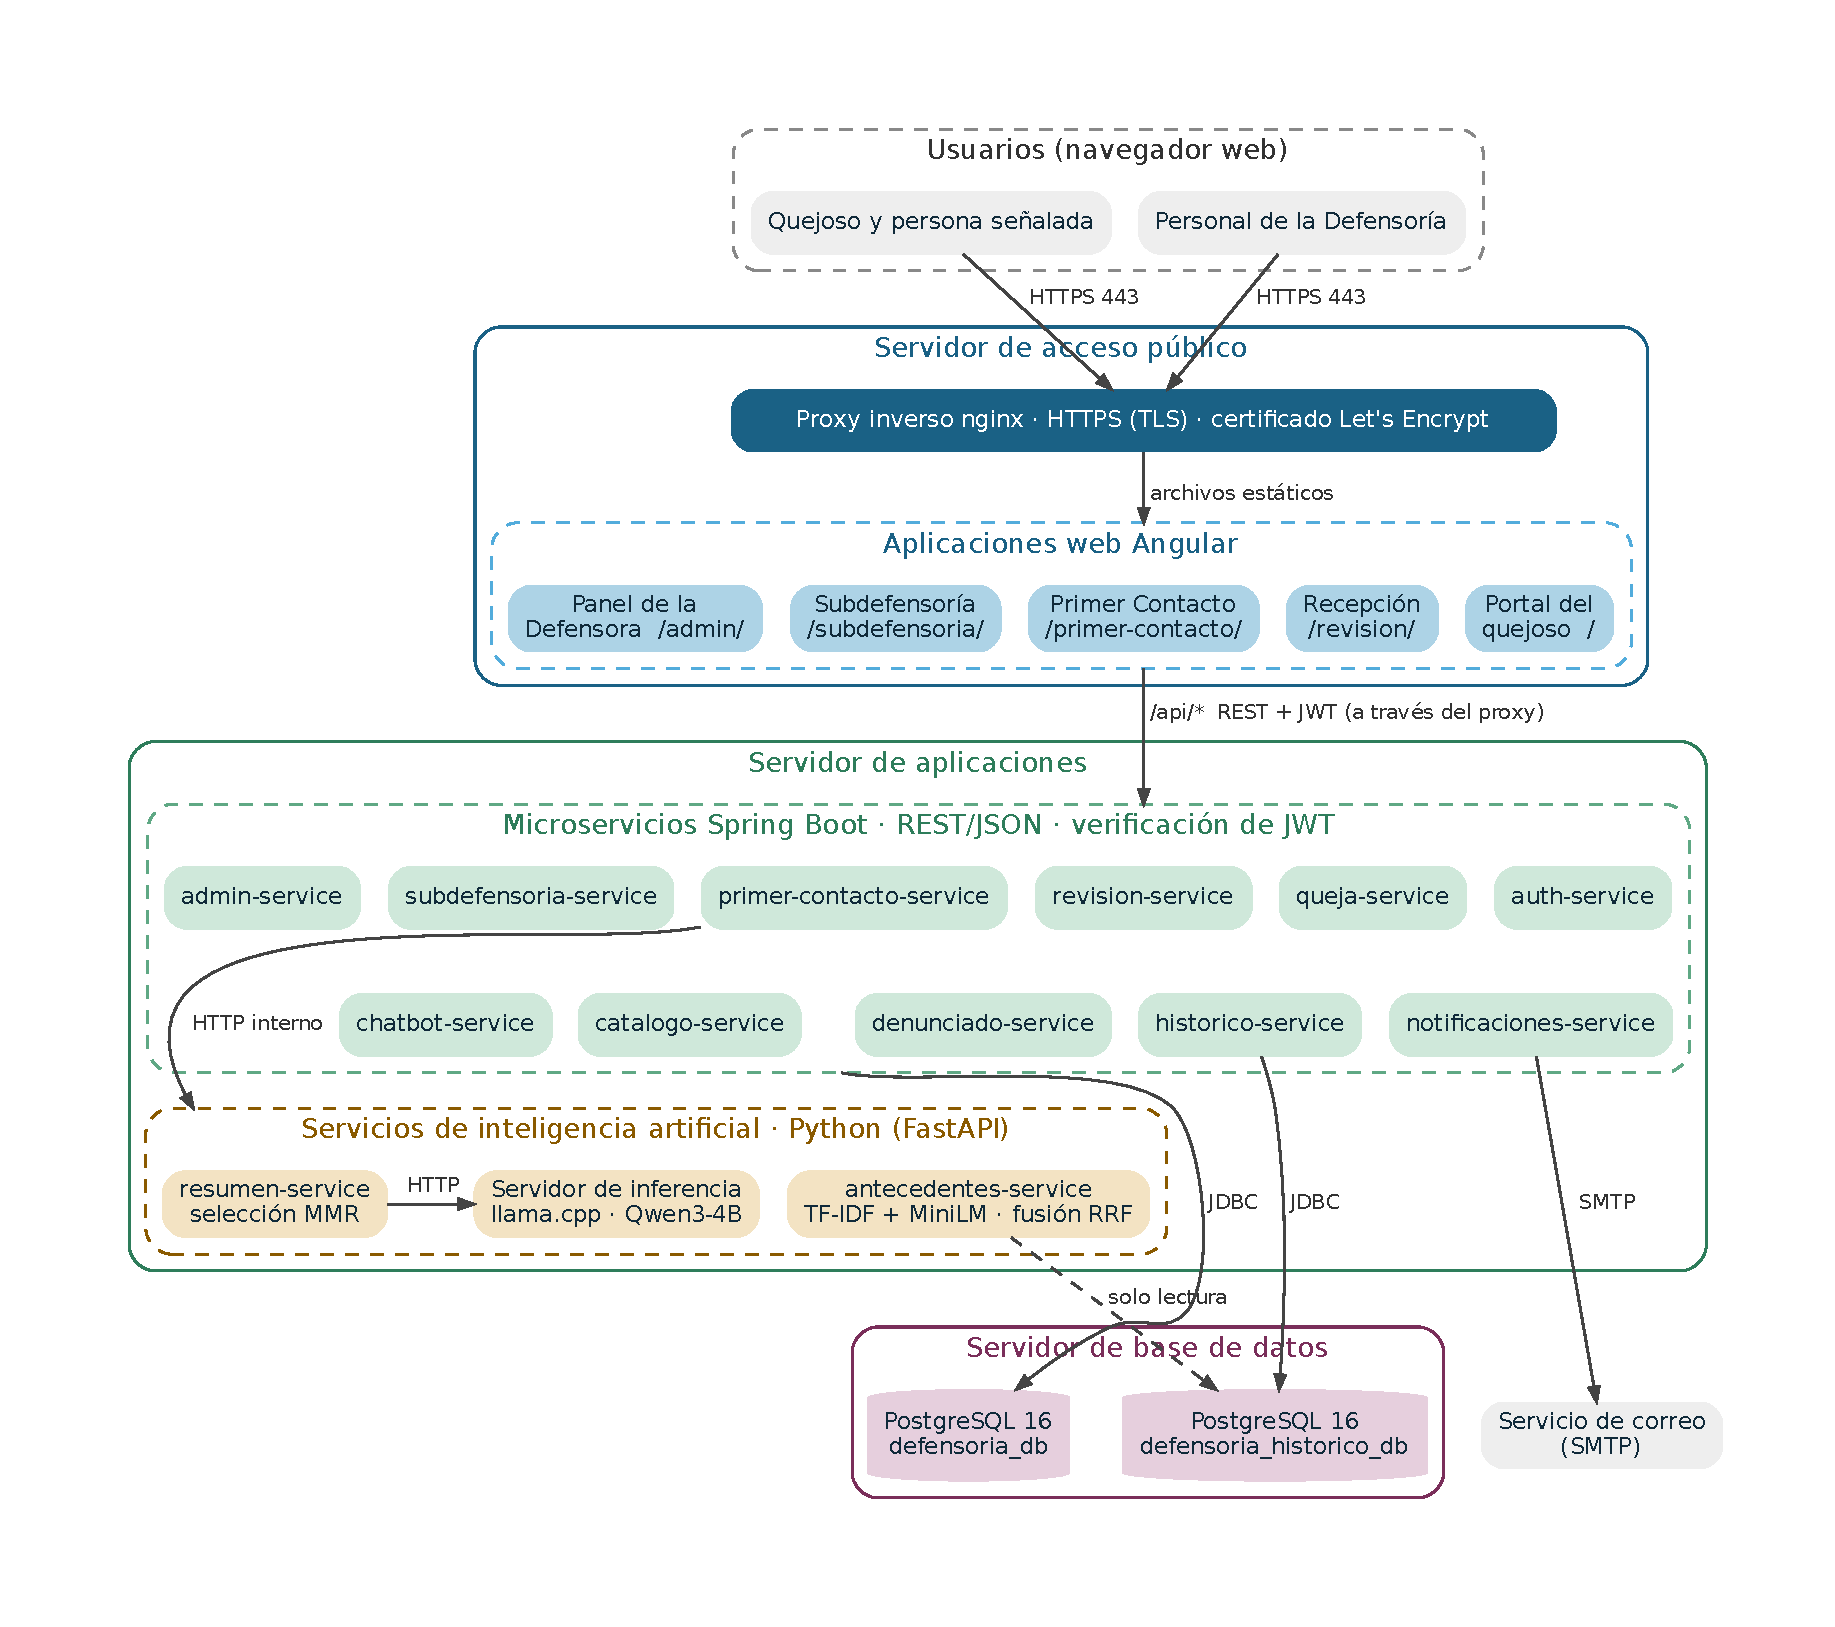
\includegraphics[width=\textwidth]{images/arquitectura.pdf}
	\caption{Arquitectura de la plataforma}
	\label{fig:arquitectura}
\end{figure}

\textbf{Servidor de acceso público.} Es el único expuesto a Internet. Un proxy inverso nginx recibe todas las peticiones por HTTPS, con un certificado de Let's Encrypt, y sirve las cinco aplicaciones web desarrolladas con Angular: el portal del quejoso y los paneles de Recepción, Primer Contacto, Subdefensoría y la Defensora, cada uno publicado en su propia ruta. Las peticiones a la interfaz de programación (\texttt{/api/*}) se reenvían al microservicio correspondiente. Como las aplicaciones y la interfaz de programación se publican bajo el mismo dominio, el navegador las trata como un mismo origen, lo que simplifica la seguridad del lado del cliente.

\textbf{Servidor de aplicaciones.} Aloja once microservicios desarrollados con Spring Boot y tres servicios de inteligencia artificial desarrollados en Python. Cada microservicio atiende un área del procedimiento y se comunica mediante peticiones REST con intercambio de datos en formato JSON. La Tabla~\ref{tab:microservicios} resume su responsabilidad. Los servicios de inteligencia artificial solo son accesibles desde la red interna: el microservicio de Primer Contacto les solicita los antecedentes y los resúmenes, y el servicio de resúmenes, a su vez, consulta al servidor de inferencia que ejecuta el modelo Qwen3 mediante llama.cpp.

\textbf{Servidor de base de datos.} Contiene dos bases de datos PostgreSQL 16: \texttt{defensoria\_db}, con la información operativa de la plataforma, y \texttt{defensoria\_historico\_db}, con las quejas históricas de la Defensoría. Sus puertos solo aceptan conexiones del servidor de aplicaciones.

\rowcolors{2}{rowblue}{white}
\small
\renewcommand{\arraystretch}{1.2}
\setlength{\tabcolsep}{4pt}
\begin{longtable}{|L{4.6cm}|L{11.0cm}|}
	\hiderowcolors\caption{Microservicios y servicios de la plataforma}
	\label{tab:microservicios} \\ \showrowcolors
	\hline
	\rowcolor{headerblue}
	\headercell{Servicio} & \headercell{Responsabilidad} \\
	\hline
	\endfirsthead
	\hline
	\rowcolor{headerblue}
	\headercell{Servicio} & \headercell{Responsabilidad} \\
	\hline
	\endhead
	\texttt{auth-service} & Sesión del quejoso: activación de la cuenta, inicio de sesión, recuperación de contraseña y perfil. Emite los tokens de los quejosos. \\ \hline
	\texttt{queja-service} & Registro de quejas, con o sin cuenta; consulta y edición de las quejas propias, evidencias y respuesta a acuerdos de conciliación. \\ \hline
	\texttt{revision-service} & Bandeja de Recepción: validación, rechazo, turnado, registro manual, historial exportable y emisión de acuerdos. \\ \hline
	\texttt{primer-contacto-service} & Expedientes de análisis, citas, oficios, dictámenes, remisiones y solicitudes a la persona señalada; integra los servicios de antecedentes y de resúmenes. \\ \hline
	\texttt{subdefensoria-service} & Expedientes de investigación, oficios de solicitud de información, control de plazos, recordatorios y acuerdos de conclusión. \\ \hline
	\texttt{denunciado-service} & Registro de la versión de los hechos de la persona señalada y de sus evidencias. \\ \hline
	\texttt{admin-service} & Sesión del personal, cuentas y roles, panel de supervisión de la Defensora, plantillas, respaldos y bitácora. Emite los tokens del personal. \\ \hline
	\texttt{notificaciones-service} & Envío de correos electrónicos y centro de notificaciones de cada usuario. \\ \hline
	\texttt{catalogo-service} & Catálogo de dependencias y unidades académicas y de instancias de remisión. \\ \hline
	\texttt{chatbot-service} & Menú de preguntas frecuentes del portal público y su administración. \\ \hline
	\texttt{historico-service} & Consulta de la información histórica de quejas. \\ \hline
	\texttt{antecedentes-service} & Búsqueda híbrida de antecedentes con TF-IDF y MiniLM sobre las quejas vigentes e históricas (solo lectura). \\ \hline
	\texttt{resumen-service} & Selección extractiva de fragmentos mediante MMR y solicitud de la redacción del resumen al modelo generativo. \\ \hline
	Servidor de inferencia & Ejecución del modelo Qwen3-4B mediante llama.cpp. \\ \hline
\end{longtable}
\normalsize
\setlength{\tabcolsep}{6pt}
\renewcommand{\arraystretch}{1}

\textbf{Seguridad.} La autenticación se basa en tokens JWT firmados. El servicio de autenticación emite los tokens de los quejosos y el de administración los del personal; el resto de los microservicios únicamente los verifican y aplican la autorización según el rol del usuario en cada operación. Las contraseñas se almacenan cifradas mediante una función de resumen. En la red, cada servidor solo acepta conexiones del servidor que le antecede: el de aplicaciones, del de acceso público, y el de base de datos, del de aplicaciones.

\textbf{Comunicación entre servicios.} La comunicación es síncrona sobre HTTP. Además de las peticiones que llegan a través del proxy, existen llamadas internas entre servicios: Primer Contacto envía a Subdefensoría los expedientes dictaminados como procedentes y varios servicios solicitan al servicio de notificaciones el envío de correos. Una falla en un servicio auxiliar, como el de notificaciones o los de inteligencia artificial, no impide que la operación principal se complete (requerimientos RNF-Q04 y RNF-G02).

\textbf{Despliegue.} Todos los componentes se ejecutan en contenedores administrados con Podman, lo que permite actualizar cada servicio de manera independiente.

\section{Diseño de la base de datos}
\label{sec:bd}
La información operativa de la plataforma se almacena en la base de datos \texttt{defensoria\_db}, administrada con PostgreSQL 16. El esquema consta de 29 tablas organizadas en cinco módulos que siguen las etapas del procedimiento: el núcleo de quejas, Primer Contacto, la respuesta de la persona señalada, Subdefensoría, y la administración y los catálogos.

Las tablas se crean a partir de las entidades que declara cada microservicio, de modo que el esquema corresponde directamente al código de la plataforma. Cada tabla tiene un microservicio responsable de su escritura. Dentro de un mismo servicio, las relaciones se declaran como llaves foráneas; entre servicios distintos, en cambio, se emplean \emph{referencias lógicas}: el registro hijo guarda el folio o el identificador del registro padre y la integridad se verifica en la lógica del servicio. Esta decisión mantiene independientes a los microservicios, a cambio de que la base de datos no impida por sí sola una referencia inválida entre módulos.

La Figura~\ref{fig:er_general} presenta el diagrama entidad-relación de la base de datos. Para que el esquema completo pueda leerse en una sola página, presentada en orientación horizontal, de cada tabla se muestran sus atributos clave: la llave primaria, las llaves foráneas, las referencias lógicas y los atributos referenciados por otras tablas, con su tipo de dato. Las tablas se distinguen por color según su módulo. Los atributos restantes de cada tabla y las relaciones de menor nivel ---como la referencia de cada cita, nota o dictamen al analista que la registró, o la cita reprogramada a partir de otra--- se presentan en los diagramas por módulo del Anexo~\ref{anx:base_datos}.

\begin{sidewaysfigure}
	\centering
	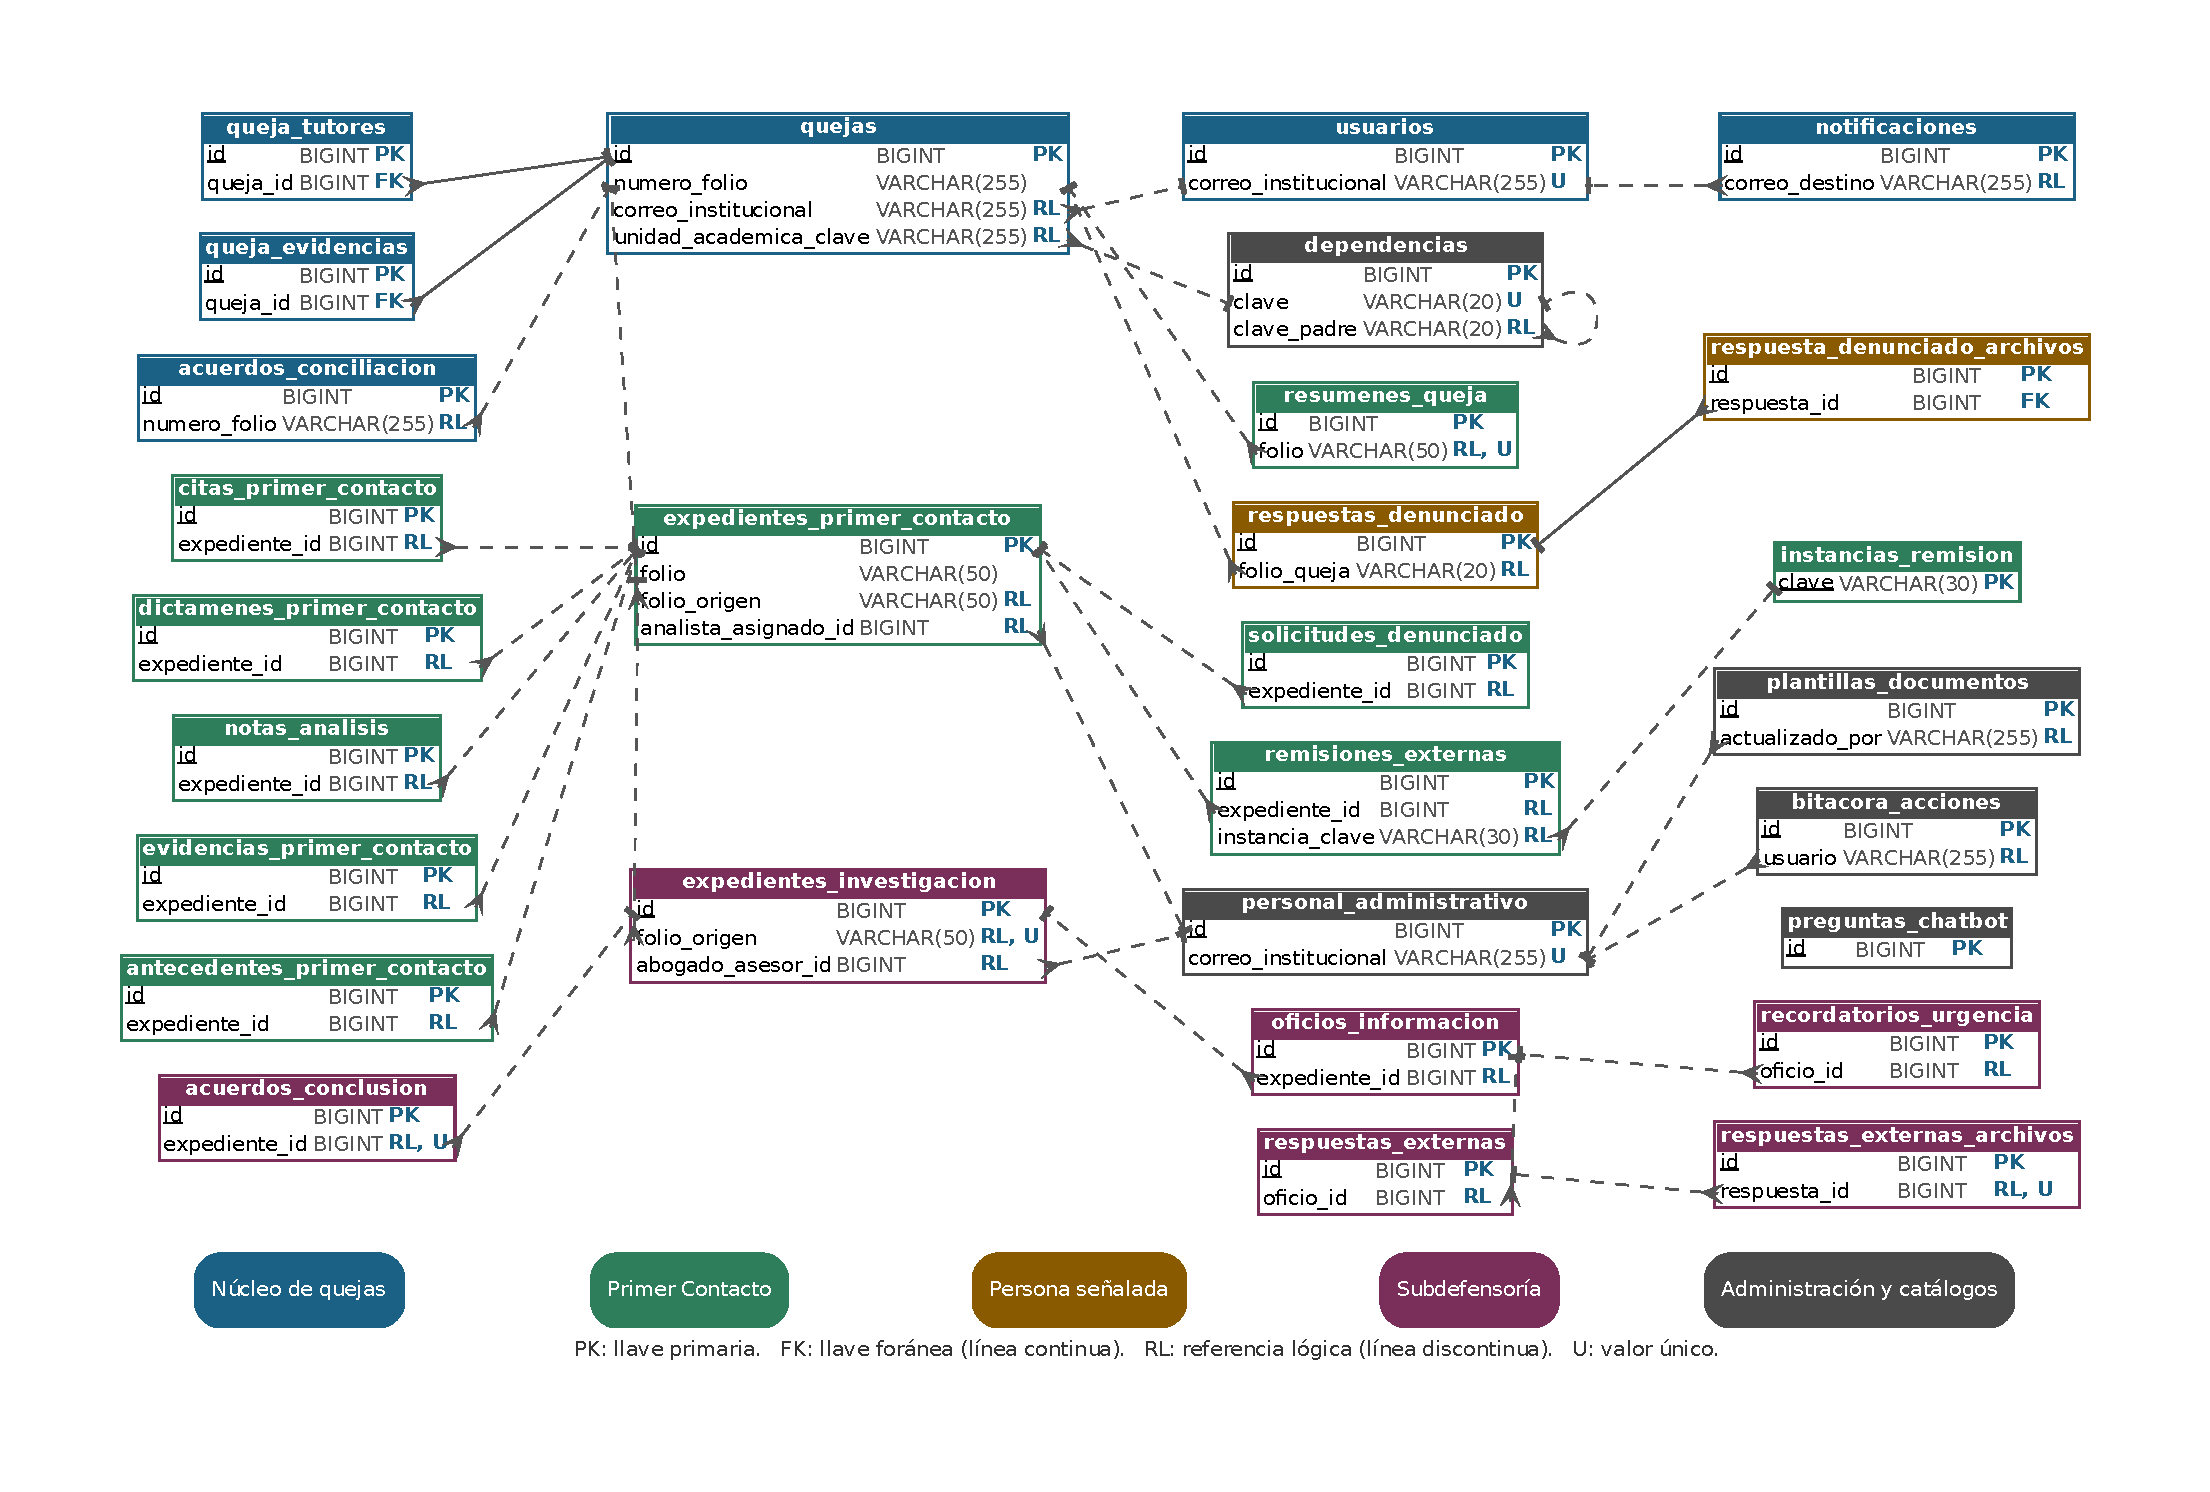
\includegraphics[width=23cm,height=14.6cm,keepaspectratio]{images/er_general.pdf}
	\caption{Diagrama entidad-relación de la base de datos (atributos clave)}
	\label{fig:er_general}
\end{sidewaysfigure}

Algunas tablas se relacionan con el resto del esquema mediante el correo electrónico y no mediante un identificador: \texttt{notificaciones} guarda el correo del destinatario, y \texttt{bitacora\_acciones} y \texttt{plantillas\_documentos} guardan el correo institucional de la persona del personal que realizó la acción o la actualización. La tabla \texttt{dependencias} se relaciona consigo misma para representar la jerarquía de dependencias del Instituto. Por último, \texttt{preguntas\_chatbot} es independiente: almacena el contenido del menú de ayuda del portal público y no depende de ningún otro registro.

El expediente de una queja recorre tres tablas principales, una por cada etapa del procedimiento. La tabla \texttt{quejas} conserva la queja tal como la presentó el quejoso y su paso por Recepción; cuando Recepción la turna, se crea un registro en \texttt{expedientes\_primer\_contacto}, que guarda el folio de la queja original; y cuando Primer Contacto la dictamina como procedente, se crea un registro en \texttt{expedientes\_investigacion}, que guarda el folio de Primer Contacto. Las demás tablas de cada módulo ---citas, dictámenes, oficios, recordatorios, acuerdos--- dependen de alguno de estos tres expedientes. Por esta razón, a continuación se presenta el diccionario de datos de estas tres tablas. En el diccionario se emplea la siguiente notación para la columna \emph{Clave}: PK, llave primaria; FK, llave foránea; RL, referencia lógica; y U, restricción de unicidad.

\subsection{Tablas principales}

\rowcolors{2}{rowblue}{white}
\footnotesize
\renewcommand{\arraystretch}{1.15}
\setlength{\tabcolsep}{4pt}
\begin{longtable}{|L{3.9cm}|L{2.4cm}|L{0.9cm}|L{1.2cm}|L{6.6cm}|}
	\hiderowcolors\caption{Diccionario de datos de la tabla \texttt{quejas}}
	\label{tab:cap3_dic_quejas} \\ \showrowcolors
	\hline
	\rowcolor{headerblue}
	\headercell{Columna} & \headercell{Tipo} & \headercell{Nulo} & \headercell{Clave} & \headercell{Descripción} \\
	\hline
	\endfirsthead
	\hline
	\rowcolor{headerblue}
	\headercell{Columna} & \headercell{Tipo} & \headercell{Nulo} & \headercell{Clave} & \headercell{Descripción} \\
	\hline
	\endhead
		\texttt{id} & BIGINT & No & PK & Identificador único del registro, generado automáticamente. \\ \hline
		\texttt{numero\_\allowbreak{}folio} & VARCHAR(255) & No &  & Folio de seguimiento que se entrega al quejoso. \\ \hline
		\texttt{correo\_\allowbreak{}institucional} & VARCHAR(255) & No & RL & Correo del quejoso; junto con el folio permite consultar la queja y activar la cuenta. \\ \hline
		\texttt{estatus} & VARCHAR(255) & Sí &  & Estatus de la queja (RECIBIDA, EN\_VALIDACION, RECHAZADA, TURNADA, entre otros). \\ \hline
		\texttt{motivo} & VARCHAR(255) & No &  & Motivo de la queja. \\ \hline
		\texttt{descripcion} & TEXT & Sí &  & Narrativa de los hechos redactada por el quejoso. \\ \hline
		\texttt{unidad\_\allowbreak{}academica\_\allowbreak{}clave} & VARCHAR(255) & Sí & RL & Clave de la unidad académica involucrada, tomada del catálogo. \\ \hline
		\texttt{fecha\_\allowbreak{}creacion} & TIMESTAMP & Sí &  & Fecha y hora en que se registró la queja. \\ \hline
		\texttt{fecha\_\allowbreak{}hechos} & DATE & Sí &  & Fecha en que ocurrieron los hechos. \\ \hline
		\texttt{nombre\_\allowbreak{}quejoso} & VARCHAR(255) & Sí &  & Nombre del quejoso. \\ \hline
		\texttt{apellido1\_\allowbreak{}quejoso} & VARCHAR(255) & Sí &  & Primer apellido del quejoso. \\ \hline
		\texttt{apellido2\_\allowbreak{}quejoso} & VARCHAR(255) & Sí &  & Segundo apellido del quejoso. \\ \hline
		\texttt{numero\_\allowbreak{}identificacion\_\allowbreak{}quejoso} & VARCHAR(255) & Sí &  & Número de boleta o de empleado del quejoso. \\ \hline
		\texttt{tipo\_\allowbreak{}identificacion\_\allowbreak{}quejoso} & VARCHAR(255) & Sí &  & Tipo de identificación del quejoso. \\ \hline
		\texttt{fecha\_\allowbreak{}nacimiento\_\allowbreak{}quejoso} & DATE & Sí &  & Fecha de nacimiento del quejoso, usada para identificar a menores de edad. \\ \hline
		\texttt{nombre\_\allowbreak{}denunciado} & VARCHAR(255) & Sí &  & Nombre de la persona señalada. \\ \hline
		\texttt{apellido1\_\allowbreak{}denunciado} & VARCHAR(255) & Sí &  & Primer apellido de la persona señalada. \\ \hline
		\texttt{apellido2\_\allowbreak{}denunciado} & VARCHAR(255) & Sí &  & Segundo apellido de la persona señalada. \\ \hline
		\texttt{folio\_\allowbreak{}primer\_\allowbreak{}contacto} & VARCHAR(255) & Sí &  & Folio asignado en Primer Contacto. \\ \hline
		\texttt{ruta\_\allowbreak{}evidencia} & VARCHAR(255) & Sí &  & Ruta de la evidencia principal de la queja. \\ \hline
		\texttt{aviso\_\allowbreak{}privacidad\_\allowbreak{}aceptado} & BOOLEAN & Sí &  & Indica si se aceptó el aviso de privacidad. \\ \hline
		\texttt{aviso\_\allowbreak{}privacidad\_\allowbreak{}fecha} & TIMESTAMP & Sí &  & Fecha y hora de aceptación del aviso de privacidad. \\ \hline
		\texttt{aviso\_\allowbreak{}privacidad\_\allowbreak{}version} & VARCHAR(255) & Sí &  & Versión del aviso de privacidad aceptada. \\ \hline
		\texttt{origen\_\allowbreak{}registro} & VARCHAR(255) & Sí &  & Punto de acceso por el que ingresó la queja (público, autenticado o manual). \\ \hline
		\texttt{motivo\_\allowbreak{}rechazo} & TEXT & Sí &  & Motivos y observaciones del rechazo. \\ \hline
		\texttt{validado\_\allowbreak{}por} & VARCHAR(255) & Sí & RL & Correo de la persona de Recepción que validó la queja. \\ \hline
		\texttt{area\_\allowbreak{}turnada} & VARCHAR(255) & Sí &  & Área a la que Recepción turnó la queja. \\ \hline
		\texttt{fecha\_\allowbreak{}turnado} & TIMESTAMP & Sí &  & Fecha y hora del turnado. \\ \hline
		\texttt{tutor\_\allowbreak{}id} & BIGINT & Sí & FK & Tutor asociado a la queja, cuando el quejoso es menor de edad. \\ \hline
		\texttt{defensor\_\allowbreak{}asignado} & VARCHAR(255) & Sí &  & Defensor o analista al que se asignó la queja al turnarla. \\ \hline
		\texttt{comentarios\_\allowbreak{}recepcion} & TEXT & Sí &  & Comentarios de Recepción al turnar la queja. \\ \hline
		\texttt{fecha\_\allowbreak{}validacion} & TIMESTAMP & Sí &  & Fecha y hora de la validación por Recepción. \\ \hline
		\texttt{revisando\_\allowbreak{}por} & VARCHAR(255) & Sí &  & Correo de la persona de Recepción que tiene tomada la queja. \\ \hline
		\texttt{revisando\_\allowbreak{}por\_\allowbreak{}nombre} & VARCHAR(255) & Sí &  & Nombre de la persona de Recepción que tiene tomada la queja. \\ \hline
		\texttt{fecha\_\allowbreak{}inicio\_\allowbreak{}revision} & TIMESTAMP & Sí &  & Fecha y hora en que Recepción tomó la queja para revisarla. \\ \hline
		\texttt{estatus\_\allowbreak{}previo\_\allowbreak{}revision} & VARCHAR(255) & Sí &  & Estatus que tenía la queja antes de que Recepción la tomara. \\ \hline
		\texttt{numero\_\allowbreak{}oficio} & VARCHAR(255) & Sí &  & Número del oficio. \\ \hline
		\texttt{fecha\_\allowbreak{}recepcion\_\allowbreak{}fisica} & DATE & Sí &  & Fecha de recepción del documento físico. \\ \hline
		\texttt{tipo\_\allowbreak{}documento\_\allowbreak{}fisico} & VARCHAR(255) & Sí &  & Tipo del documento físico recibido. \\ \hline
		\texttt{ubicacion\_\allowbreak{}fisica\_\allowbreak{}expediente} & VARCHAR(255) & Sí &  & Ubicación física del expediente en papel. \\ \hline
		\texttt{tipo\_\allowbreak{}usuario\_\allowbreak{}manual} & VARCHAR(255) & Sí &  & Tipo de usuario capturado en el registro manual. \\ \hline
		\texttt{telefono\_\allowbreak{}contacto} & VARCHAR(255) & Sí &  & Teléfono de contacto del quejoso. \\ \hline
\end{longtable}
\normalsize
\setlength{\tabcolsep}{6pt}
\renewcommand{\arraystretch}{1}

\rowcolors{2}{rowblue}{white}
\footnotesize
\renewcommand{\arraystretch}{1.15}
\setlength{\tabcolsep}{4pt}
\begin{longtable}{|L{3.9cm}|L{2.4cm}|L{0.9cm}|L{1.2cm}|L{6.6cm}|}
	\hiderowcolors\caption{Diccionario de datos de la tabla \texttt{expedientes\_primer\_contacto}}
	\label{tab:cap3_dic_expedientes_primer_contacto} \\ \showrowcolors
	\hline
	\rowcolor{headerblue}
	\headercell{Columna} & \headercell{Tipo} & \headercell{Nulo} & \headercell{Clave} & \headercell{Descripción} \\
	\hline
	\endfirsthead
	\hline
	\rowcolor{headerblue}
	\headercell{Columna} & \headercell{Tipo} & \headercell{Nulo} & \headercell{Clave} & \headercell{Descripción} \\
	\hline
	\endhead
		\texttt{id} & BIGINT & No & PK & Identificador único del registro, generado automáticamente. \\ \hline
		\texttt{folio} & VARCHAR(50) & No &  & Folio del expediente en Primer Contacto. \\ \hline
		\texttt{folio\_\allowbreak{}origen} & VARCHAR(50) & No & RL & Folio de la queja original. \\ \hline
		\texttt{tema} & VARCHAR(200) & Sí &  & Tema o motivo de la queja. \\ \hline
		\texttt{descripcion\_\allowbreak{}hechos} & TEXT & Sí &  & Narrativa de los hechos copiada de la queja. \\ \hline
		\texttt{fecha\_\allowbreak{}recepcion\_\allowbreak{}origen} & VARCHAR(50) & Sí &  & Fecha de recepción de la queja original. \\ \hline
		\texttt{prioridad} & VARCHAR(30) & Sí &  & Prioridad del expediente (baja, media, alta o urgente). \\ \hline
		\texttt{quejoso\_\allowbreak{}nombre} & VARCHAR(200) & Sí &  & Nombre del quejoso. \\ \hline
		\texttt{quejoso\_\allowbreak{}correo} & VARCHAR(150) & Sí &  & Correo electrónico del quejoso. \\ \hline
		\texttt{unidad\_\allowbreak{}academica} & VARCHAR(200) & Sí &  & Unidad académica relacionada. \\ \hline
		\texttt{estatus} & VARCHAR(40) & No &  & Estatus del análisis (TURNADA, EN\_ANALISIS, PROCEDENTE, IMPROCEDENTE, REMITIDA, entre otros). \\ \hline
		\texttt{fecha\_\allowbreak{}inicio\_\allowbreak{}analisis} & TIMESTAMP & Sí &  & Fecha y hora en que inició el análisis. \\ \hline
		\texttt{analista\_\allowbreak{}analisis\_\allowbreak{}id} & BIGINT & Sí &  & Identificador del analista que inició el análisis. \\ \hline
		\texttt{analista\_\allowbreak{}analisis\_\allowbreak{}nombre} & VARCHAR(150) & Sí &  & Nombre del analista que inició el análisis. \\ \hline
		\texttt{analista\_\allowbreak{}asignado\_\allowbreak{}id} & BIGINT & Sí & RL & Identificador del analista al que Recepción turnó el expediente. \\ \hline
		\texttt{analista\_\allowbreak{}asignado\_\allowbreak{}nombre} & VARCHAR(150) & Sí &  & Nombre del analista asignado. \\ \hline
		\texttt{fecha\_\allowbreak{}creacion} & TIMESTAMP & No &  & Fecha y hora de creación del registro. \\ \hline
		\texttt{fecha\_\allowbreak{}actualizacion} & TIMESTAMP & Sí &  & Fecha y hora de la última actualización. \\ \hline
		\texttt{folio\_\allowbreak{}subdefensoria} & VARCHAR(50) & Sí & U & Folio del expediente de investigación en Subdefensoría. \\ \hline
		\texttt{quejoso\_\allowbreak{}id} & BIGINT & Sí &  & Identificador de la cuenta del quejoso, si existe. \\ \hline
		\texttt{quejoso\_\allowbreak{}telefono} & VARCHAR(30) & Sí &  & Teléfono del quejoso. \\ \hline
		\texttt{quejoso\_\allowbreak{}tipo\_\allowbreak{}usuario} & VARCHAR(50) & Sí &  & Tipo de usuario del quejoso (alumno, personal, etc.). \\ \hline
\end{longtable}
\normalsize
\setlength{\tabcolsep}{6pt}
\renewcommand{\arraystretch}{1}

\rowcolors{2}{rowblue}{white}
\footnotesize
\renewcommand{\arraystretch}{1.15}
\setlength{\tabcolsep}{4pt}
\begin{longtable}{|L{3.9cm}|L{2.4cm}|L{0.9cm}|L{1.2cm}|L{6.6cm}|}
	\hiderowcolors\caption{Diccionario de datos de la tabla \texttt{expedientes\_investigacion}}
	\label{tab:cap3_dic_expedientes_investigacion} \\ \showrowcolors
	\hline
	\rowcolor{headerblue}
	\headercell{Columna} & \headercell{Tipo} & \headercell{Nulo} & \headercell{Clave} & \headercell{Descripción} \\
	\hline
	\endfirsthead
	\hline
	\rowcolor{headerblue}
	\headercell{Columna} & \headercell{Tipo} & \headercell{Nulo} & \headercell{Clave} & \headercell{Descripción} \\
	\hline
	\endhead
		\texttt{id} & BIGINT & No & PK & Identificador único del registro, generado automáticamente. \\ \hline
		\texttt{folio} & VARCHAR(50) & No & U & Folio del expediente en Subdefensoría. \\ \hline
		\texttt{folio\_\allowbreak{}origen} & VARCHAR(50) & No & RL, U & Folio del expediente en Primer Contacto. \\ \hline
		\texttt{folio\_\allowbreak{}queja} & VARCHAR(50) & Sí &  & Folio de la queja original. \\ \hline
		\texttt{quejoso\_\allowbreak{}nombre} & VARCHAR(150) & Sí &  & Nombre del quejoso. \\ \hline
		\texttt{quejoso\_\allowbreak{}correo} & VARCHAR(150) & Sí &  & Correo electrónico del quejoso. \\ \hline
		\texttt{unidad\_\allowbreak{}academica} & VARCHAR(100) & Sí &  & Unidad académica relacionada. \\ \hline
		\texttt{asunto} & VARCHAR(200) & Sí &  & Asunto o tema del documento. \\ \hline
		\texttt{descripcion\_\allowbreak{}hechos} & TEXT & Sí &  & Narrativa de los hechos de la queja. \\ \hline
		\texttt{fecha\_\allowbreak{}admision} & DATE & No &  & Fecha en que el expediente se admitió en Subdefensoría. \\ \hline
		\texttt{abogado\_\allowbreak{}asesor\_\allowbreak{}id} & BIGINT & Sí & RL & Identificador del abogado de Subdefensoría asignado (personal administrativo). \\ \hline
		\texttt{abogado\_\allowbreak{}asesor\_\allowbreak{}nombre} & VARCHAR(150) & Sí &  & Nombre del abogado asignado, conservado para consulta. \\ \hline
		\texttt{estatus} & VARCHAR(30) & No &  & Etapa de la investigación (RECIBIDO, EN\_INVESTIGACION, EN\_ESPERA\_OFICIO, CONCLUIDO, entre otras). \\ \hline
		\texttt{observaciones\_\allowbreak{}analista} & TEXT & Sí &  & Observaciones del analista de Primer Contacto al turnar. \\ \hline
		\texttt{prioridad} & VARCHAR(10) & Sí &  & Prioridad del expediente (baja, media, alta o urgente). \\ \hline
		\texttt{fecha\_\allowbreak{}creacion} & TIMESTAMP & No &  & Fecha y hora de creación del registro. \\ \hline
		\texttt{fecha\_\allowbreak{}actualizacion} & TIMESTAMP & Sí &  & Fecha y hora de la última actualización. \\ \hline
\end{longtable}
\normalsize
\setlength{\tabcolsep}{6pt}
\renewcommand{\arraystretch}{1}

\noindent\textbf{Nota:} los diagramas entidad-relación de cada módulo con todas sus columnas y el diccionario de datos completo de las 29 tablas se presentan en el Anexo~\ref{anx:base_datos}.


%% Capitulo 4. Trabajo realizado (solo estructura; el material previo
%% esta en sections/material_cap4/ para usarlo al construirlo)
\chapter{Trabajo realizado}
\label{cap:trabajo_realizado}
\label{cap:analisis_diseno}
\label{cap:implementacion}
\label{cap:modulos}
\pendiente{Introducción del capítulo: qué se construyó y cómo se organiza este capítulo.}

\section{Ciclo de vida del expediente}
\label{sec:ciclo_vida}
\pendiente{Diagrama de estados de la queja y descripción del flujo entre áreas.}

\section{Componentes de inteligencia artificial}
\label{sec:diseno_ia}
\pendiente{Cómo se construyeron la búsqueda de antecedentes y la generación de resúmenes.}

\section{Pantallas principales de la plataforma}
\label{sec:pantallas}
\pendiente{Presentar las diez pantallas más importantes: qué hace cada una, cómo se hizo y a qué requerimientos responde.}

\subsection{Pantalla 1}
\pendiente{Captura, descripción y requerimientos que cubre.}

\subsection{Pantalla 2}
\pendiente{Captura, descripción y requerimientos que cubre.}

\subsection{Pantalla 3}
\pendiente{Captura, descripción y requerimientos que cubre.}

\subsection{Pantalla 4}
\pendiente{Captura, descripción y requerimientos que cubre.}

\subsection{Pantalla 5}
\pendiente{Captura, descripción y requerimientos que cubre.}

\subsection{Pantalla 6}
\pendiente{Captura, descripción y requerimientos que cubre.}

\subsection{Pantalla 7}
\pendiente{Captura, descripción y requerimientos que cubre.}

\subsection{Pantalla 8}
\pendiente{Captura, descripción y requerimientos que cubre.}

\subsection{Pantalla 9}
\pendiente{Captura, descripción y requerimientos que cubre.}

\subsection{Pantalla 10}
\pendiente{Captura, descripción y requerimientos que cubre.}

\section{Despliegue}
\label{sec:despliegue}
\pendiente{Contenedores, servidores y publicación de la plataforma.}


%% Capitulo 5. Pruebas
\chapter{Pruebas}
	\label{cap:pruebas}
	Este capítulo documenta la verificación de la plataforma: la estrategia con que se diseñaron las
	pruebas y los casos y resultados de cada característica de calidad. Las pruebas se organizan siguiendo el modelo ISO/IEC 25010 \cite{iso25010} con que se
	clasificaron los requerimientos no funcionales (Tabla~\ref{tab:rnf}), en siete secciones:
	funcionalidad, mantenibilidad, usabilidad, fiabilidad, seguridad, capacidad y confidencialidad. Cada
	caso de prueba indica el requerimiento que verifica, lo que permite rastrear cada requerimiento
	hasta la evidencia que lo respalda.

	Una advertencia de método acompaña a todo el capítulo: probar no demuestra la ausencia de defectos,
	solo reduce el riesgo de que existan \cite{myers_testing}. Por eso las pruebas se priorizaron según
	el daño que causaría cada falla, y los resultados se reportan tal como se obtuvieron, incluidas las
	pruebas que fallaron y las que siguen pendientes de ejecutarse.

	\section{Estrategia de pruebas}
	\label{sec:estrategia_pruebas}
	\subsection{Niveles y técnicas}
	La estrategia sigue el modelo en V, en el que cada nivel de prueba verifica el artefacto del nivel de
	diseño correspondiente \cite{istqb_foundation}:

	\begin{itemize}
		\item \textbf{Pruebas de componente (unitarias).} Verifican una clase de reglas o de servicio de
		forma aislada, sustituyendo sus dependencias por objetos simulados. Se aplican solo a la lógica que
		toma decisiones; no se prueban métodos de acceso, DTO ni repositorios generados.
		\item \textbf{Pruebas de integración.} Verifican la colaboración de un servicio con su base de
		datos, su configuración de seguridad y los servicios que invoca. Se siguió una estrategia
		ascendente: primero cada servicio con su base, después los pares de servicios.
		\item \textbf{Pruebas de sistema.} Recorren los casos de uso de extremo a extremo sobre el sistema
		desplegado en un entorno de pruebas.
		\item \textbf{Pruebas de aceptación.} Ejecutadas por personal de la Defensoría, o por personas que
		actúan cada rol, bajo supervisión del equipo (pruebas alfa).
	\end{itemize}

	Según la información disponible para diseñarlas, las pruebas son de \textbf{caja blanca} ---se
	diseñan a partir del código, como las unitarias y la verificación estática de permisos--- o de
	\textbf{caja negra} ---se diseñan a partir de la especificación y se ejecutan contra la interfaz
	pública, como las de seguridad dinámica y de confidencialidad---. Según su forma de ejecución, son
	\textbf{estáticas}, si analizan el código o la configuración sin ejecutarlos, o
	\textbf{dinámicas}, si ejecutan el sistema. Para diseñar los datos de entrada se emplearon las
	técnicas de particiones de equivalencia, análisis de valores límite, tablas de decisión y transición
	de estados \cite{myers_testing}; por ejemplo, el plazo de 90 días se prueba con 89, 90 y 91 días, y
	la máquina de estados de la queja con cada transición permitida y con las prohibidas.

	\subsection{Prioridad basada en riesgo}
	No es viable probar todas las combinaciones de entrada, de modo que el esfuerzo se asignó según el
	daño que causaría cada falla. Son de prioridad P1 los riesgos de acceso indebido a datos personales,
	de ruptura del ciclo de estatus, de atención simultánea de una queja por dos recepcionistas, de falla
	en el paso de expedientes entre áreas y de exposición del tráfico o de los secretos; de prioridad
	P2, los errores en plazos y datos obligatorios, la pérdida de respaldos y la caída de servicios
	auxiliares; y de prioridad P3, la lentitud y las pantallas confusas.

	\subsection{Entorno y criterios}
	Las pruebas dinámicas se ejecutan en un entorno de pruebas y no en producción: una base PostgreSQL~16
	dedicada, sembrada con los datos de referencia y con la carga masiva de quejas sintéticas, los mismos
	artefactos que se despliegan y una cuenta de prueba por rol. Las pruebas estáticas y unitarias no
	necesitan el sistema levantado. Se definieron los siguientes criterios:

	\begin{itemize}
		\item \textbf{Entrada:} el código compila sin errores y el entorno de pruebas está disponible.
		\item \textbf{Salida:} todos los casos P1 ejecutados y aprobados, al menos el 90~\% de los P2
		ejecutados, ningún defecto crítico o alto abierto, cobertura de al menos 70~\% en las clases de
		reglas, percentil 95 menor a 1~s en la prueba de carga y puntaje SUS de al menos 68.
		\item \textbf{Suspensión:} si un defecto crítico bloquea más del 30~\% de los casos, se detiene la
		ejecución hasta corregirlo.
	\end{itemize}

	\section{Pruebas de funcionalidad}
	\label{sec:pruebas_funcionalidad}
	Las pruebas de funcionalidad verifican la adecuación funcional: que las reglas de negocio y los
	casos de uso se comporten como se especificaron.

	\subsection{Pruebas unitarias}
	Se escribieron pruebas unitarias con JUnit~5 y Mockito para los diez microservicios Java
	desarrollados para la plataforma \cite{junit5, mockito}. Las pruebas no levantan el contexto de
	Spring ni requieren base de datos o red: las dependencias se sustituyen por objetos simulados, lo que
	permite ejecutarlas en segundos en cada compilación. Siguen el patrón preparar--actuar--verificar, incluyen
	un mensaje en cada aserción y se diseñaron con particiones de equivalencia y valores límite. La
	Tabla~\ref{tab:pruebas_unitarias} resume su alcance.

	\rowcolors{2}{rowblue}{white}
	\small
	\renewcommand{\arraystretch}{1.2}
	\setlength{\tabcolsep}{4pt}
	\begin{longtable}{|p{3.4cm}|L{1.3cm}|L{9.8cm}|}
		\hiderowcolors\caption{Pruebas unitarias por microservicio}
		\label{tab:pruebas_unitarias} \\ \showrowcolors
		\hline
		\rowcolor{headerblue}
		\headercell{Servicio} & \headercell{Casos} & \headercell{Qué verifican} \\
		\hline
		\endfirsthead
		\hline
		\rowcolor{headerblue}
		\headercell{Servicio} & \headercell{Casos} & \headercell{Qué verifican} \\
		\hline
		\endhead
		\texttt{quejas-service} & 112 & Validadores del registro público: correo en dos niveles, fechas,
		nombres, boleta, tutor y archivos por firma binaria; edición, corrección y cancelación; conciliación
		(RN-Q01 a RN-Q12) \\ \hline
		\texttt{primer-contacto-service} & 55 & Citas sin empalmes, plazo y rango máximo de consulta,
		token de respuesta; dictamen con Subdefensoría caída; sincronización de estatus; motor de
		antecedentes (RN-PC01 a RN-PC04) \\ \hline
		\texttt{admin-service} & 36 & Cuentas del personal y protección de la última cuenta de
		administración; bitácora con IP real; plantillas; respaldos en carpeta temporal; tablero (RN-A01 a
		RN-A04, RNF-A07) \\ \hline
		\texttt{auth-service} & 36 & Inicio de sesión, recuperación con código (cinco intentos, diez
		minutos), política de contraseñas, activación y emisión del token (RN-Q06 a RN-Q08) \\ \hline
		\texttt{revision-service} & 36 & Toma atómica entre recepcionistas, regreso, turnado idempotente,
		ventanilla e historial (RN-R01 a RN-R07, RNF-R06) \\ \hline
		\texttt{denunciado-service} & 29 & Todas las reglas del registro de la versión de la persona
		señalada (RF-D01) \\ \hline
		\texttt{subdefensoria-service} & 24 & Días hábiles (10 y 5), semáforo y alertas de vencimiento,
		archivo de respuesta (RN-SD01, RN-SD02) \\ \hline
		\texttt{notificaciones-service} & 20 & Centro de notificaciones e inyección de encabezados en el
		correo (CWE-93) \\ \hline
		\texttt{catalogo-service} & 8 & Alta, edición e importación de Excel tolerante a errores
		(RNF-A04) \\ \hline
		\texttt{chatbot-service} & 8 & Menú agrupado y administración de preguntas \\ \hline
		\textbf{Total} & \textbf{364} & \\ \hline
	\end{longtable}
	\normalsize

	\textbf{Resultado.} Los 364 casos se ejecutaron con Maven y resultaron aprobados (0 fallas, 0
	errores). La única prueba que requería base de datos ---la carga del contexto de Primer Contacto---
	se etiquetó como de integración y se excluye de la ejecución unitaria, para que la suite no dependa
	del entorno. Posteriormente se incorporaron ocho casos de resiliencia, descritos en la
	Sección~\ref{sec:pruebas_fiabilidad}; al cierre documentado se señala que
	FIA-05 y FIA-06 están implementadas, pero pendientes de su primera ejecución.
	Por esa razón, esos ocho casos no se suman a las 364 pruebas aprobadas.

	\subsection{Pruebas de integración y de sistema}
	La Tabla~\ref{tab:pruebas_integracion} lista los casos de integración y de sistema de prioridad P1 y
	P2 con su resultado. Los que tienen evidencia se ejecutaron durante el desarrollo de cada módulo con
	guiones y con el navegador; los marcados como pendientes forman parte de la suite de sistema que se
	ejecutará en el entorno de pruebas antes de la entrega a la Defensoría.

	\rowcolors{2}{rowblue}{white}
	\small
	\renewcommand{\arraystretch}{1.2}
	\setlength{\tabcolsep}{4pt}
	\begin{longtable}{|p{1.2cm}|L{6.2cm}|L{2.2cm}|L{2.0cm}|L{2.9cm}|}
		\hiderowcolors\caption{Pruebas de integración y de sistema}
		\label{tab:pruebas_integracion} \\ \showrowcolors
		\hline
		\rowcolor{headerblue}
		\headercell{ID} & \headercell{Qué se verifica} & \headercell{Requerimiento} &
		\headercell{Tipo} & \headercell{Resultado} \\
		\hline
		\endfirsthead
		\hline
		\rowcolor{headerblue}
		\headercell{ID} & \headercell{Qué se verifica} & \headercell{Requerimiento} &
		\headercell{Tipo} & \headercell{Resultado} \\
		\hline
		\endhead
		IT-06 & Dos recepcionistas abren la misma queja al mismo tiempo; solo una la obtiene &
		RNF-R06, RN-R03 & Dinámica, CN & Aprobada (10 de 10 intentos concurrentes) \\ \hline
		IT-20 & Activar una cuenta solo con un par folio--correo válido & RN-Q06 & Dinámica, CB &
		Aprobada en prueba unitaria; dinámica pendiente \\ \hline
		IT-22 & La queja turnada aparece en la bandeja de Primer Contacto & CU-REC-05, CU-PC-01 & Dinámica,
		CN & Aprobada en el sistema desplegado \\ \hline
		IT-23 & El dictamen competente crea el expediente en Subdefensoría & CU-PC-06, CU-SD-01 & Dinámica,
		CN & Aprobada en entorno local con la base de pruebas \\ \hline
		IT-24 & El cambio de estatus en Primer Contacto se refleja en la tabla de quejas & RN-R01 &
		Dinámica, CB & Aprobada en prueba unitaria de sincronización \\ \hline
		IT-09 & Los indicadores del panel de la Defensora coinciden con datos sembrados en PostgreSQL~16 &
		CU-ADM-03 & Dinámica, CB & Aprobada \\ \hline
		IT-11 & Inicio de sesión unificado: siete escenarios (sin sesión, enlace antiguo, Defensora en
		Recepción, cierre de sesión, recepcionista hacia el panel de la Defensora, entre otros) & CU-ADM-07,
		RNF-R02 & Dinámica, CN & Aprobada (7 de 7) \\ \hline
		IT-12 & Registro de la persona señalada con datos válidos, nombres con dígitos, ejecutable
		renombrado, credencial PDF o de 4~MB, tres credenciales y sin aviso & RF-D01, RNF-G08 & Dinámica,
		CB & Aprobada (19 de 19) \\ \hline
		REN-02 & Carga masiva de quejas sintéticas por el registro público, con credencial y evidencias &
		CU-QJ-07 & Dinámica, CN & Aprobada (170 quejas) \\ \hline
		ST-01 a ST-14 & Recorridos de extremo a extremo por actor, automatizados con Playwright & Casos de
		uso & Dinámica, CN & Pendiente: suite por automatizar; recorridos verificados manualmente \\ \hline
	\end{longtable}
	\normalsize

	\textbf{Compilación de producción.} Las cinco aplicaciones web se compilan con la configuración de
	producción, que falla si un componente excede su presupuesto de tamaño o si una plantilla hace
	referencia a un elemento inexistente. Las cinco compilan sin errores.

	\section{Pruebas de mantenibilidad}
	\label{sec:pruebas_mantenibilidad}
	La mantenibilidad se verificó con pruebas estáticas de caja blanca sobre el código Java de ocho de
	los diez servicios (225 archivos), y con la cobertura de las pruebas unitarias. Primer Contacto y
	Subdefensoría se analizaron con las mismas reglas de forma informativa.

	\subsection{Guía de estilo}
	El proyecto adoptó como guía de estilo el Google Java Style Guide \cite{google_java_style}, con cuatro
	desviaciones que reflejan lo que el código ya seguía de forma consistente, para no reformatear todo
	el proyecto sin aportar calidad ---sangría de 4 espacios en lugar de 2, líneas de 120 columnas en lugar de 100, guion bajo
	permitido en los nombres de paquete y el registrador \texttt{log} en minúsculas---. La guía se codificó como
	configuración de Checkstyle: las reglas \textbf{obligatorias} deben cumplirse sin excepción y las
	\textbf{recomendadas} se reportan como deuda técnica.



	La Tabla~\ref{tab:pruebas_mantenibilidad} resume los casos y sus resultados.

	\rowcolors{2}{rowblue}{white}
	\small
	\renewcommand{\arraystretch}{1.2}
	\setlength{\tabcolsep}{4pt}
	\begin{longtable}{|p{1.2cm}|L{5.5cm}|L{3.1cm}|L{4.7cm}|}
		\hiderowcolors\caption{Pruebas de mantenibilidad}
		\label{tab:pruebas_mantenibilidad} \\ \showrowcolors
		\hline
		\rowcolor{headerblue}
		\headercell{ID} & \headercell{Qué se verifica} & \headercell{Criterio} & \headercell{Resultado} \\
		\hline
		\endfirsthead
		\hline
		\rowcolor{headerblue}
		\headercell{ID} & \headercell{Qué se verifica} & \headercell{Criterio} & \headercell{Resultado} \\
		\hline
		\endhead
		MAN-01 & Reglas obligatorias de la guía: nombre de archivo, sin tabuladores, sin importaciones con
		comodín, llaves siempre, un enunciado por línea, una variable por declaración, nombres, sin
		\texttt{System.out} ni excepciones ignoradas, \texttt{equals} con \texttt{hashCode} & 0
		violaciones & Fallida: 4 violaciones en 225 archivos (tres en \texttt{RevisionQuejaService}: dos
		enunciados en una línea, dos variables en una declaración y un \texttt{if} sin llaves; una
		importación estática con comodín en \texttt{RespuestaDenunciadoService}) \\ \hline
		MAN-02 & Métricas: complejidad ciclomática $\leq 15$, NPath $\leq 400$, método $\leq 80$ líneas,
		$\leq 8$ parámetros, acoplamiento de salida $\leq 30$, archivo $\leq 800$ líneas & Se reporta como
		deuda & Informativa: 5 métodos con complejidad mayor a 15, 117 tipos públicos sin Javadoc, 90 líneas
		de más de 120 columnas \\ \hline
		MAN-03 & Cobertura de líneas en los paquetes de servicios, validaciones y utilerías, medida con
		JaCoCo & $\geq 70~\%$ por servicio & Pendiente de su primera ejecución (el reporte se
		genera en cada ejecución de las pruebas) \\ \hline
		MAN-04 & Cada servicio publica su contrato OpenAPI & 10 de 10 & Aprobada (Primer Contacto y
		Subdefensoría lo incorporaron al cierre) \\ \hline
	\end{longtable}
	\normalsize

	El cumplimiento global de las reglas obligatorias es de cuatro violaciones en 225 archivos: corregirlas
	permite aprobar MAN-01. La deuda reportada por MAN-02 no es bloqueante, pero indica dónde conviene
	concentrar la refactorización; los métodos más complejos están en los servicios de revisión y de
	seguimiento, que concentran la lógica de los tableros.

	\section{Pruebas de usabilidad}
	\label{sec:pruebas_usabilidad}
	La usabilidad no puede verificarse por completo con herramientas automáticas, porque depende de la
	experiencia de personas concretas. Se combinaron por ello mediciones automáticas de accesibilidad con
	pruebas con usuarios. La Tabla~\ref{tab:pruebas_usabilidad} resume los casos.

	\rowcolors{2}{rowblue}{white}
	\small
	\renewcommand{\arraystretch}{1.2}
	\setlength{\tabcolsep}{4pt}
	\begin{longtable}{|p{1.2cm}|L{5.6cm}|L{2.2cm}|L{2.6cm}|L{2.9cm}|}
		\hiderowcolors\caption{Pruebas de usabilidad}
		\label{tab:pruebas_usabilidad} \\ \showrowcolors
		\hline
		\rowcolor{headerblue}
		\headercell{ID} & \headercell{Qué se verifica} & \headercell{Requerimiento} &
		\headercell{Criterio} & \headercell{Resultado} \\
		\hline
		\endfirsthead
		\hline
		\rowcolor{headerblue}
		\headercell{ID} & \headercell{Qué se verifica} & \headercell{Requerimiento} &
		\headercell{Criterio} & \headercell{Resultado} \\
		\hline
		\endhead
		USA-01 & Cuestionario SUS a cinco usuarios después de las pruebas alfa \cite{brooke_sus} & RNF-G09 &
		Puntaje $\geq 68$ & Pendiente: sesión alfa con la Defensoría \\ \hline
		USA-02 & Tareas cronometradas: presentar una queja, turnar, agendar una cita y dictaminar & RNF-Q05,
		RNF-A05 & Tiempo y errores por tarea & Pendiente: sesión alfa \\ \hline
		USA-03 & Accesibilidad básica de los portales: contraste, etiquetas y uso con teclado, medida con
		Lighthouse & RNF-G09 & Puntuación $\geq 0.85$ & Configurada; informativa hasta definir el umbral
		por portal \\ \hline
		USA-04 & El portal del quejoso permite presentar la queja completa desde un teléfono & RNF-Q01 &
		Flujo completo & Pendiente de verificación formal; diseño adaptable implementado \\ \hline
		USA-05 & El formulario de queja se presenta en pasos numerados con previsualización de archivos &
		RNF-Q05 & Cumple & Aprobada por inspección \\ \hline
		USA-06 & Toda operación muestra éxito o error; sin fallos silenciosos & RNF-Q07 & Cumple & Aprobada
		por inspección; se propone automatizarla con Playwright \\ \hline
		USA-07 & Cada indicador del panel de la Defensora abre la lista filtrada & RNF-A05 & Cumple &
		Aprobada en revisión con capturas de las cinco pantallas \\ \hline
	\end{longtable}
	\normalsize

	La validación cualitativa más importante ocurrió durante el desarrollo: las sesiones de revisión con
	el personal produjeron cambios concretos ---la redacción jurídica de los requisitos de admisión, el
	paso de dos a cinco preguntas en la validación, la matrícula en dos pasos y el rediseño completo de
	Primer Contacto y del panel de la Defensora---, lo que equivale a varias iteraciones de prueba de
	usabilidad informal. La medición cuantitativa con SUS queda como criterio de salida de la etapa de
	aceptación.

	\section{Pruebas de fiabilidad}
	\label{sec:pruebas_fiabilidad}
	Las pruebas de fiabilidad verifican la tolerancia a fallos ---que el fallo de un componente no
	detenga a los demás--- y la recuperabilidad ---que los datos puedan restaurarse---. Las primeras se
	implementaron como pruebas unitarias que simulan un servicio caído; las segundas, como guiones que
	operan sobre bases desechables.

	\rowcolors{2}{rowblue}{white}
	\small
	\renewcommand{\arraystretch}{1.2}
	\setlength{\tabcolsep}{4pt}
	\begin{longtable}{|p{1.2cm}|L{5.6cm}|L{2.2cm}|L{2.6cm}|L{2.9cm}|}
		\hiderowcolors\caption{Pruebas de fiabilidad}
		\label{tab:pruebas_fiabilidad} \\ \showrowcolors
		\hline
		\rowcolor{headerblue}
		\headercell{ID} & \headercell{Qué se verifica} & \headercell{Requerimiento} &
		\headercell{Criterio} & \headercell{Resultado} \\
		\hline
		\endfirsthead
		\hline
		\rowcolor{headerblue}
		\headercell{ID} & \headercell{Qué se verifica} & \headercell{Requerimiento} &
		\headercell{Criterio} & \headercell{Resultado} \\
		\hline
		\endhead
		FIA-05 & Con el servicio de notificaciones sin conexión o respondiendo 500, los avisos de queja
		creada, al tutor, de cambio de estatus y al personal no propagan la excepción (4 casos) & RNF-Q04 &
		Ninguna excepción se propaga & Implementada; pendiente de su primera ejecución \\ \hline
		FIA-06 & Con el servicio de notificaciones caído, el correo de observaciones y los avisos de
		Recepción no impiden el regreso de la queja (4 casos) & RNF-R04 & Ninguna excepción se propaga &
		Implementada; pendiente de su primera ejecución \\ \hline
		FIA-07 & La importación del catálogo con filas mal formadas reporta un resumen y no falla en bloque
		& RNF-A04 & Resumen de creadas, actualizadas y con error & Aprobada \\ \hline
		FIA-04 & Con Subdefensoría caída al dictaminar, el dictamen se conserva y puede reenviarse &
		RN-PC03 & El dictamen no se pierde & Aprobada (prueba unitaria) \\ \hline
		FIA-03 & Respaldo manual, descarga y restauración en una base desechable & RNF-G04, CU-ADM-05 & Sin
		errores de \texttt{psql}; tablas principales con filas & Pendiente de ejecución en el entorno de
		pruebas \\ \hline
		FIA-01 & Detener un contenedor auxiliar mientras se usa el sistema & RNF-Q04 & El resto opera &
		Aprobada en operación (incidentes de la Sección~\ref{sec:incidentes}) \\ \hline
		FIA-02 & Reiniciar el servidor de aplicación & RNF-G04 & Los contenedores se levantan solos &
		Aprobada en operación \\ \hline
	\end{longtable}
	\normalsize

	Las pruebas FIA-05 y FIA-06 son el ejemplo más claro de cómo un incidente se convirtió en prueba. El
	defecto descrito en la Sección~\ref{sec:incidentes} ---peticiones colgadas por una llamada sin tiempo
	de espera--- se habría detectado con una prueba que simulara el servicio caído. Las pruebas usan un
	cliente HTTP simulado que lanza un error de conexión o un error 500 y verifican que ningún método del
	cliente de notificaciones propague la excepción hacia el servicio que lo invoca. La restauración
	(FIA-03) es la prueba de mayor impacto de esta sección: un respaldo que no puede restaurarse no es un
	respaldo, y la única forma de saberlo es restaurarlo. El guion genera un respaldo desde el panel,
	lo descarga, lo restaura en una base nueva y verifica que las tablas de quejas, personal y
	dependencias tengan filas.

	\section{Pruebas de seguridad}
	\label{sec:pruebas_seguridad}
	La seguridad se verificó en dos planos complementarios. En el plano estático, se extrajo del código la
	matriz completa de roles por punto de acceso y se comparó con las reglas que exigen los
	requerimientos. En el plano dinámico, la misma matriz se recorre contra el sistema en ejecución con un
	token por rol.

	\subsection{Matriz de permisos extraída del código}
	Un guion recorre los controladores de ocho de los diez servicios ---Primer Contacto y Subdefensoría
	declaran sus permisos solo en la cadena de filtros y se verifican en la prueba dinámica---, lee las rutas, los
	métodos HTTP, las anotaciones \texttt{@PreAuthorize} y las reglas públicas de la cadena de filtros, y
	genera una matriz de 92 puntos de acceso con los roles que cada uno admite. Un segundo guion compara
	esa matriz con un archivo de reglas que traduce los requerimientos a expresiones sobre las rutas ---por
	ejemplo, ``\texttt{/api/admin/seguridad/(respaldos|restaurar)} solo admite a la Defensora''--- y
	reporta cada diferencia. Al ser estática, la prueba puede ejecutarse con cada cambio del código y detecta, antes del
	despliegue, un punto de acceso nuevo que se haya publicado con permisos de más.

	La primera ejecución encontró seis diferencias. Cuatro correspondían a los respaldos y la
	restauración, que el código abre al rol \texttt{DEFENSOR} mientras que la redacción original del
	requerimiento RNF-A06 los reservaba a un rol técnico de administración. Las otras dos
	correspondían a la consulta y emisión de acuerdos de conciliación, que el código abre también a
	Subdefensoría y a la Defensora, mientras que la redacción original de RN-R02 reservaba todo el
	servicio de revisión a Recepción. En ambos casos el análisis concluyó que el código reflejaba la
	decisión de diseño vigente ---por convención con la Defensoría, la administración corresponde a la
	Defensora, y la conciliación es una actuación de varias áreas---, de modo que se corrigió la redacción de los requerimientos
	(Tablas~\ref{tab:rnf} y~\ref{tab:reglas_negocio}) y el archivo de reglas, y no el código. El
	resultado ilustra un beneficio de esta prueba que va más allá de la seguridad: obliga a que el
	documento de requerimientos y el código digan lo mismo.

	\subsection{Casos de prueba de seguridad}
	La Tabla~\ref{tab:pruebas_seguridad} reúne los casos de seguridad con su resultado.

	\rowcolors{2}{rowblue}{white}
	\small
	\renewcommand{\arraystretch}{1.2}
	\setlength{\tabcolsep}{4pt}
	\begin{longtable}{|p{1.2cm}|L{5.6cm}|L{2.2cm}|L{2.6cm}|L{2.9cm}|}
		\hiderowcolors\caption{Pruebas de seguridad}
		\label{tab:pruebas_seguridad} \\ \showrowcolors
		\hline
		\rowcolor{headerblue}
		\headercell{ID} & \headercell{Qué se verifica} & \headercell{Requerimiento} &
		\headercell{Criterio} & \headercell{Resultado} \\
		\hline
		\endfirsthead
		\hline
		\rowcolor{headerblue}
		\headercell{ID} & \headercell{Qué se verifica} & \headercell{Requerimiento} &
		\headercell{Criterio} & \headercell{Resultado} \\
		\hline
		\endhead
		SEG-07 & Matriz de permisos extraída del código contra las reglas de los requerimientos (34 puntos
		de acceso regulados de 92) & RNF-A06, RN-R02, RNF-R02, RNF-Q01, RNF-Q02, RN-Q12 & 0 diferencias &
		Fallida en la línea base (6 diferencias); resuelta al alinear los requerimientos \\ \hline
		SEG-01 & La matriz en vivo: sin token, 401 o 403; con un rol no permitido, 403; con el permitido,
		la petición pasa el filtro & RN-R02, RNF-A06 & 0 accesos indebidos & Pendiente de ejecución en el
		entorno de pruebas \\ \hline
		SEG-10 & Las rutas de Primer Contacto y Subdefensoría exigen token (antes eran públicas) & RN-R02 &
		403 sin token & Aprobada en el servidor: consulta, PDF de oficios y evidencias responden 403 sin
		token \\ \hline
		IT-04 & Un quejoso no puede consultar ni editar la queja de otra persona cambiando el folio & RN-Q11
		& 404 & Aprobada por revisión de código (búsqueda por folio y correo del token) \\ \hline
		SEG-08 & El token vence a la hora (\texttt{exp} $-$ \texttt{iat} $= 3\,600$) y un token alterado se
		rechaza & RNF-Q06 & 3\,600~s; 401 o 403 & Aprobada por configuración y prueba unitaria de emisión;
		dinámica pendiente \\ \hline
		SEG-09 & Restaurar sin \texttt{"confirmar": true} se rechaza & RNF-A03 & Respuesta 4xx & Probable falla
		por revisión de código: se rechaza con una excepción genérica que se traduce en 500, no en 400 \\ \hline
		SEG-03 & Recorrido de rutas (\texttt{../}) en la descarga y restauración de respaldos & RNF-A06 &
		Distinto de 200 & Fallida por revisión de código: el nombre de archivo no se valida contra la carpeta
		de respaldos (riesgo bajo: solo cuentas de administración) \\ \hline
		SEG-05 & Secretos ---contraseña de la base, clave de firma de tokens, credenciales de correo--- en el
		repositorio & RNF-G07 & 0 hallazgos & Fallida: residen en texto plano en los archivos de
		configuración \\ \hline
		SEG-04 & Dependencias Maven y npm con vulnerabilidades altas o críticas con parche & RNF-G07 & 0 &
		Pendiente de su primera ejecución \\ \hline
		SEG-02 & Escaneo pasivo de vulnerabilidades web de los cinco portales & RNF-G06 & Sin alertas
		altas & Pendiente (informativa) \\ \hline
		SEG-11 & Los puertos de los servicios y de la base no son alcanzables desde Internet & RNF-G06 &
		Conexión rechazada & Aprobada en operación (reglas en la tabla \texttt{raw}) \\ \hline
	\end{longtable}
	\normalsize

	Tres resultados requieren acción. El más importante es SEG-05: las contraseñas y la clave de firma
	de los tokens están en los archivos de configuración versionados, y la rama de producción del
	repositorio pudo clonarse sin credenciales. La corrección consiste en rotar esos secretos, pasarlos a
	variables de entorno del servidor y retirarlos del historial del repositorio. SEG-03 se corrige
	verificando que la ruta normalizada del archivo permanezca dentro de la carpeta de respaldos, y SEG-09
	con un manejador que traduzca la falta de confirmación a una respuesta 400.

	\section{Pruebas de capacidad}
	\label{sec:pruebas_capacidad}
	La capacidad se verifica en dos dimensiones: el tamaño máximo de una petición, que determina cuántas
	evidencias puede adjuntar un quejoso, y el número de usuarios concurrentes. Las pruebas de tamaño
	envían formularios multiparte vacíos a propósito, con un relleno del tamaño deseado, de modo que no
	crean quejas en el entorno.

	\rowcolors{2}{rowblue}{white}
	\small
	\renewcommand{\arraystretch}{1.2}
	\setlength{\tabcolsep}{4pt}
	\begin{longtable}{|p{1.2cm}|L{5.6cm}|L{2.2cm}|L{2.6cm}|L{2.9cm}|}
		\hiderowcolors\caption{Pruebas de capacidad}
		\label{tab:pruebas_capacidad} \\ \showrowcolors
		\hline
		\rowcolor{headerblue}
		\headercell{ID} & \headercell{Qué se verifica} & \headercell{Requerimiento} &
		\headercell{Criterio} & \headercell{Resultado} \\
		\hline
		\endfirsthead
		\hline
		\rowcolor{headerblue}
		\headercell{ID} & \headercell{Qué se verifica} & \headercell{Requerimiento} &
		\headercell{Criterio} & \headercell{Resultado} \\
		\hline
		\endhead
		CAP-01 & Una petición de 95~MB atraviesa el proxy & RNF-Q03 & Distinto de 413 & Pendiente de
		ejecución \\ \hline
		CAP-02 & Una petición de 105~MB es rechazada por el proxy & RNF-Q03 & 413 & Pendiente de ejecución \\ \hline
		CAP-03, CAP-04 & Lo mismo directamente contra el servicio de quejas & RNF-Q03 & Distinto de 413 / 413
		& Pendiente de ejecución \\ \hline
		CAP-06 & Coherencia entre el requerimiento y la configuración de cada servicio & RNF-Q03 & Iguales
		& Observada y resuelta: el requerimiento indicaba 60~MB y los servicios aceptan 100~MB; se actualizó
		el requerimiento \\ \hline
		CAP-07 & Una queja con seis archivos, uno de 12.5~MB, se registra sin terminar el contenedor &
		RNF-Q03 & Respuesta 200 & Aprobada tras el redimensionamiento de memoria \\ \hline
		CAP-05 & 50 usuarios virtuales concurrentes sobre las consultas públicas (catálogo, menú del
		chatbot, consulta por folio) & RNF-G05 & p95 $< 1$~s; errores $< 1~\%$ & Pendiente de ejecución
		con k6 \\ \hline
	\end{longtable}
	\normalsize

	La prueba CAP-07 merece un comentario. El límite de tamaño de una petición no es solo una cifra de
	configuración: como las evidencias se guardan como contenido binario en la base, cada megabyte
	recibido se copia varias veces en memoria. Un límite de 100~MB por petición exige que el servicio
	tenga memoria para varias copias de esa petición, y la prueba con archivos reales fue la que reveló
	que el contenedor original no la tenía. Por eso RNF-Q03 se verifica con dos tipos de prueba: la de
	límites, que comprueba el rechazo, y la de archivos reales, que comprueba que lo aceptado se procesa.

	\section{Pruebas de confidencialidad}
	\label{sec:pruebas_confidencialidad}
	La confidencialidad se verifica con pruebas de caja negra que observan, desde fuera del servidor, cómo
	viaja la información. Son pasivas ---no modifican datos--- y por ello pueden ejecutarse también contra
	producción. El guion usa \texttt{openssl} para negociar conexiones con cada versión de TLS y
	\texttt{curl} para revisar redirecciones y encabezados.

	\rowcolors{2}{rowblue}{white}
	\small
	\renewcommand{\arraystretch}{1.2}
	\setlength{\tabcolsep}{4pt}
	\begin{longtable}{|p{1.2cm}|L{5.6cm}|L{2.2cm}|L{2.6cm}|L{2.9cm}|}
		\hiderowcolors\caption{Pruebas de confidencialidad}
		\label{tab:pruebas_confidencialidad} \\ \showrowcolors
		\hline
		\rowcolor{headerblue}
		\headercell{ID} & \headercell{Qué se verifica} & \headercell{Requerimiento} &
		\headercell{Criterio} & \headercell{Resultado} \\
		\hline
		\endfirsthead
		\hline
		\rowcolor{headerblue}
		\headercell{ID} & \headercell{Qué se verifica} & \headercell{Requerimiento} &
		\headercell{Criterio} & \headercell{Resultado} \\
		\hline
		\endhead
		CON-01 & Una petición HTTP se redirige a HTTPS & RNF-Q02 & 301 a \texttt{https} & Aprobada por
		configuración; dinámica pendiente \\ \hline
		CON-02 & Se aceptan TLS 1.2 y 1.3 & RNF-Q02 & Negociación exitosa & Aprobada por configuración
		(\texttt{ssl\_protocols}) \\ \hline
		CON-03 & Se rechazan TLS 1.0 y 1.1 & RNF-Q02 & Negociación fallida & Aprobada por configuración \\ \hline
		CON-04 & Certificado válido con al menos 14 días de vigencia & RNF-Q02 & Cumple & Aprobada por
		configuración (renovación automática con Certbot) \\ \hline
		CON-05 & El servidor envía el encabezado \texttt{Strict-Transport-Security} & RNF-Q02 & Presente &
		Fallida: el proxy no lo envía \\ \hline
		CON-06 & Las respuestas JSON de la API no se comprimen (mitigación de BREACH) & RNF-Q02 & Sin
		\texttt{Content-Encoding} & Aprobada por configuración \\ \hline
		CON-07 & Las rutas internas de notificaciones e ingesta responden 403 desde Internet & RNF-G06 &
		403 & Aprobada por configuración; dinámica pendiente \\ \hline
		CON-08 & El inicio de sesión no usa \textit{cookies} ni acepta credenciales en la URL; la sesión
		viaja en el encabezado \texttt{Authorization} & RNF-Q02 & Sin \texttt{Set-Cookie} & Aprobada por
		diseño \\ \hline
		CON-09 & Las evidencias de una queja solo se entregan al quejoso dueño o al personal autorizado &
		RN-Q11 & 403 o 404 para terceros & Aprobada (cubierta por IT-04 y SEG-10) \\ \hline
	\end{longtable}
	\normalsize

	La única falla, CON-05, se corrige con una línea en la configuración del servidor seguro del proxy.
	Varias pruebas figuran como aprobadas por configuración porque la configuración del proxy se revisó
	línea por línea; su ejecución dinámica, que confirma que esa configuración es la que realmente está
	cargada, queda pendiente para el entorno de pruebas.
	
	\section{Pruebas de los componentes de inteligencia artificial}
\label{sec:pruebas_ia}

La verificación de los componentes de inteligencia artificial comprendió dos tipos de actividades:
la evaluación experimental de la recuperación de antecedentes con datos sintéticos y las
pruebas funcionales y de integración realizadas sobre los servicios desplegados. En el caso de
los resúmenes se verificaron tanto la respuesta técnica del servicio como la presencia de
información relevante en una salida generada. Se distinguen expresamente las mediciones
experimentales de las comprobaciones puntuales de funcionamiento, pues una respuesta HTTP
correcta no demuestra por sí sola la calidad del contenido producido.

\subsection{Evaluación de recuperación de antecedentes}
\label{sec:pruebas_ia_antecedentes}

Se utilizaron dos conjuntos sintéticos. El primero estuvo compuesto por 200 quejas extensas,
organizadas en 25 escenarios con ocho variantes de redacción por escenario; cada queja se
empleó como consulta y la relevancia se determinó mediante su pertenencia al mismo escenario.
Para interpretar correctamente esta evaluación, debe comprobarse y dejarse explícito
si cada consulta fue excluida de la colección de candidatos. Si no se excluyó,
una coincidencia consigo misma podría sobrestimar la recuperación. La información
presentada no basta para establecer cuál fue el tratamiento aplicado.
El segundo incluyó 15 consultas contrastivas frente a 45 documentos candidatos, con un
antecedente positivo sintético por consulta y documentos distractores. Estas etiquetas
representan relaciones diseñadas para el experimento y no equivalen a una valoración jurídica
de los expedientes.

Para estudiar la combinación de los recuperadores léxico (TF-IDF) y semántico (MiniLM) se
reutilizaron los rankings calculados previamente por ambos modelos. La fusión se realizó con
\textit{Reciprocal Rank Fusion} (RRF), considerando los diez primeros candidatos de cada
recuperador y una constante de suavizado de 60. Se examinaron 101 distribuciones de peso,
desde 100\,\% léxico hasta 100\,\% semántico, con incrementos de un punto porcentual. Esta
operación recalculó la fusión sobre rankings guardados; no supuso ejecutar nuevamente MiniLM
para cada combinación ni consultar los expedientes del servidor de producción.

Se calcularon precisión en los primeros cinco resultados (P@5), exhaustividad en los primeros
diez (R@10), rango recíproco medio (MRR) y ganancia acumulada descontada normalizada
(nDCG@5), entre otras métricas. La Tabla~\ref{tab:ia_pesos_200} muestra una selección de
ponderaciones para las 200 quejas extensas.

\begin{longtable}{|p{3.8cm}|p{2.6cm}|p{2.6cm}|p{2.6cm}|}
\hiderowcolors\caption{Resultados de recuperación en 200 quejas sintéticas extensas}
\label{tab:ia_pesos_200} \\ \showrowcolors
\hline
\textbf{TF-IDF / MiniLM} & \textbf{P@5} & \textbf{R@10} & \textbf{nDCG@5} \\
\hline
\endfirsthead
\hline
\textbf{TF-IDF / MiniLM} & \textbf{P@5} & \textbf{R@10} & \textbf{nDCG@5} \\
\hline
\endhead
100\,\% / 0\,\% & 45.2\,\% & 91.5\,\% & 0.435 \\ \hline
90\,\% / 10\,\% & 52.3\,\% & 91.5\,\% & 0.496 \\ \hline
75\,\% / 25\,\% & 52.0\,\% & 91.5\,\% & 0.490 \\ \hline
50\,\% / 50\,\% & 49.7\,\% & 67.5\,\% & 0.471 \\ \hline
25\,\% / 75\,\% & 48.5\,\% & 46.5\,\% & 0.457 \\ \hline
0\,\% / 100\,\% & 33.5\,\% & 46.5\,\% & 0.325 \\ \hline
\end{longtable}

La búsqueda con predominio léxico obtuvo el mejor P@5 entre las configuraciones mostradas,
pero la diferencia entre 90\,/\,10 y 75\,/\,25 fue de solo 0.3 puntos porcentuales. En la
búsqueda más fina de 101 combinaciones, la ponderación 91\,/\,9 también alcanzó un P@5
de 52.3\,\%. Por tanto, los datos no permiten afirmar una superioridad concluyente de una
ponderación concreta. Además, el resultado depende de la métrica seleccionada: el orden más
favorable para P@5 no tiene por qué serlo para la primera posición.

La configuración final adoptada para el servicio fue 75\,\% TF-IDF y
25\,\% MiniLM en la fusión RRF ponderada. En este primer conjunto alcanzó
P@5 de 52.0\,\%, R@10 de 91.5\,\% y nDCG@5 de 0.490. La elección
no equivale a afirmar que sea la mejor ponderación para todos los escenarios: se
conserva como configuración de implementación y se reportan sus limitaciones.

La Tabla~\ref{tab:ia_pesos_contraste} resume la prueba contrastiva. En este conjunto, donde
se introdujeron diferencias de redacción y distractores, la mayor influencia del recuperador
semántico produjo una exhaustividad sustancialmente superior. Dado que solo existe
un antecedente relevante por consulta, el valor máximo teórico de P@5 es 20\,\%
cuando se devuelven cinco resultados: por ello, sus porcentajes no son directamente
comparables con los del conjunto de 200 quejas, que tiene varios documentos
relevantes por escenario. Para este segundo conjunto resultan particularmente
interpretables las métricas Hit@k y MRR; deben añadirse sus resultados solo
cuando se cuente con las salidas verificadas del experimento.

\begin{longtable}{|p{3.8cm}|p{2.6cm}|p{2.6cm}|p{2.6cm}|}
\hiderowcolors\caption{Resultados en 15 consultas sintéticas contrastivas}
\label{tab:ia_pesos_contraste} \\ \showrowcolors
\hline
\textbf{TF-IDF / MiniLM} & \textbf{P@5} & \textbf{R@10} & \textbf{nDCG@5} \\
\hline
\endfirsthead
\hline
\textbf{TF-IDF / MiniLM} & \textbf{P@5} & \textbf{R@10} & \textbf{nDCG@5} \\
\hline
\endhead
90\,\% / 10\,\% & 2.7\,\% & 13.3\,\% & 0.084 \\ \hline
75\,\% / 25\,\% & 2.7\,\% & 13.3\,\% & 0.084 \\ \hline
50\,\% / 50\,\% & 9.3\,\% & 86.7\,\% & 0.216 \\ \hline
25\,\% / 75\,\% & 9.3\,\% & 93.3\,\% & 0.219 \\ \hline
0\,\% / 100\,\% & 17.3\,\% & 93.3\,\% & 0.669 \\ \hline
\end{longtable}

En particular, la ponderación final 75/25 alcanzó P@5 de 2.7\,\%,
R@10 de 13.3\,\% y nDCG@5 de 0.084 en las consultas contrastivas.
Este resultado advierte que la configuración seleccionada puede omitir
antecedentes relevantes cuando existe poca coincidencia léxica, por lo que
debe mantenerse la revisión humana y ampliarse la evaluación de casos
parafraseados.

Los resultados evidencian un compromiso entre coincidencia léxica y recuperación semántica,
no una ponderación universalmente óptima. La diferencia entre conjuntos podría
relacionarse con el grado de coincidencia de vocabulario, las paráfrasis y la
construcción de distractores, pero estas hipótesis requieren un análisis
individual de consultas fallidas para comprobarse. La selección de pesos se examinó también mediante
particiones por escenario, con el propósito de no ajustar y medir una configuración sobre los
mismos grupos sintéticos. No obstante, el documento no especifica el número de
particiones, sus tamaños ni los resultados diferenciados de selección y evaluación,
por lo que aún no puede considerarse reproducible dicho procedimiento. Aun así, los conjuntos no han sido etiquetados por especialistas
de la Defensoría; por tanto, estas medidas describen el comportamiento experimental del
recuperador y no su precisión sobre expedientes institucionales reales.

\subsection{Funcionamiento del índice y respuesta de antecedentes}
\label{sec:pruebas_ia_indice}

En el servidor se verificó la construcción del índice sobre 1\,210 registros y la
persistencia de sus representaciones semánticas. Una actualización posterior, sin cambios
en los documentos, informó 1\,210 representaciones reutilizadas y ninguna recalculada.
El servicio informó estado listo mediante su punto de comprobación de disponibilidad.

También se ejecutaron consultas HTTP de búsqueda de antecedentes con respuesta satisfactoria
(código 200). En una consulta sintética de revisión de calificación, la API de análisis
respondió en aproximadamente 0.135 segundos; en otra consulta realizada mediante el contrato
de integración se registró un tiempo cercano a 0.111 segundos. Estas cifras son observaciones
puntuales con el índice disponible, no percentiles de latencia ni pruebas de concurrencia.

\subsection{Generación de resúmenes e integración con los servicios}
\label{sec:pruebas_ia_resumenes}

Se envió una queja sintética al servicio de resúmenes, que realiza una selección extractiva
de información y posteriormente utiliza un modelo generativo para redactar un borrador en
estilo institucional. La solicitud devolvió HTTP 200 y un tiempo total de 26.304 segundos.
Se confirmó la presencia de un texto generado y del indicador de revisión humana requerida.

La inspección del resultado permitió identificar tanto elementos conservados como omisiones.
Es una observación cualitativa de un caso, no una tasa de fidelidad o de cobertura
para el componente de generación.
Se mantuvieron las referencias a los correos electrónicos y capturas del sistema, así como
la negación de agresión física; en cambio, no se conservaron las dos fechas explícitas ni
el cambio de calificación de ocho a seis. Por tanto, esta prueba fue satisfactoria en
respuesta técnica, pero detectó una limitación de cobertura factual. No se completó en esa
prueba la atribución de las omisiones a la fase extractiva o a la edición generativa.
Para efectuar esa atribución podría compararse, incluso con entradas sintéticas,
el texto original, la selección extractiva y el borrador generado, verificando
acontecimientos, negaciones, fechas, cantidades y evidencias. Hasta disponer de
esa comparación, no corresponde atribuir la pérdida de información exclusivamente
a MMR o a Qwen3.

La evaluación efectuada no incluyó un conjunto amplio de resúmenes evaluados
mediante criterios institucionales, ni una validación formal con expedientes
reales y personal de la Defensoría de los Derechos Politécnicos. Estas actividades
no pudieron completarse debido al tiempo disponible para el desarrollo y la
presentación del Trabajo Terminal. En consecuencia, las pruebas con narrativas
sintéticas permiten comprobar la integración y detectar errores puntuales, pero
no establecer un nivel de fidelidad, cobertura o utilidad generalizable a la
operación de la Defensoría. Como trabajo futuro, se propone una evaluación con
expedientes reales debidamente autorizados y revisión de personal institucional,
con criterios explícitos para la conservación de hechos, actores, fechas,
negaciones, cantidades, evidencias y solicitudes. Este trabajo debe distinguir
las posibles omisiones de la etapa extractiva de las modificaciones introducidas
por la etapa generativa.

Después del despliegue se comprobó, mediante solicitudes al punto de salud, que el servicio
Java de Primer Contacto podía comunicarse con el servicio de resúmenes (HTTP 200) y que
este último podía comunicarse con el servidor del modelo generativo (HTTP 200). Estas
comprobaciones acreditan conectividad entre componentes, pero no constituyen una medición
de calidad del resumen ni una prueba de carga.

\subsection{Alcance de los resultados de inteligencia artificial}

Las pruebas ejecutadas permiten documentar el comportamiento de la fusión de rankings sobre
conjuntos sintéticos, la reutilización del índice y el funcionamiento de las interfaces HTTP.
Sin embargo, no demuestran que la ponderación 75/25 sea óptima sobre quejas reales ni
la conservación factual sistemática de los resúmenes. La verificación de una
salida generada no sustituye un estudio con múltiples documentos y criterios de
revisión previamente definidos. Por cuestiones de tiempo no fue posible llevar
a cabo la validación con expedientes reales ni la revisión formal por parte del
personal de la Defensoría. Este alcance debe distinguirse de las pruebas técnicas
que sí fueron ejecutadas con datos sintéticos. La evaluación institucional queda
identificada como trabajo futuro y requiere acceso autorizado a los expedientes,
definición de criterios con los especialistas y análisis independiente de las
etapas extractiva y generativa. Tampoco se documentan una prueba de concurrencia
para la inferencia ni una distribución representativa de los tiempos de respuesta.



%% Capitulo 6. Resultados obtenidos
\chapter{Resultados obtenidos}
\label{cap:resultados}

	\section{Resumen de resultados}
	\label{sec:resumen_pruebas}
	La Tabla~\ref{tab:defectos} reúne los defectos abiertos que dejaron las pruebas, con la acción
	que resuelve cada uno.



	\rowcolors{2}{rowblue}{white}
	\small
	\renewcommand{\arraystretch}{1.2}
	\setlength{\tabcolsep}{4pt}
	\begin{longtable}{|p{1.4cm}|L{5.6cm}|L{1.8cm}|L{5.7cm}|}
		\hiderowcolors\caption{Defectos abiertos y acción correctiva}
		\label{tab:defectos} \\ \showrowcolors
		\hline
		\rowcolor{headerblue}
		\headercell{Prueba} & \headercell{Defecto} & \headercell{Severidad} & \headercell{Acción} \\
		\hline
		\endfirsthead
		\hline
		\rowcolor{headerblue}
		\headercell{Prueba} & \headercell{Defecto} & \headercell{Severidad} & \headercell{Acción} \\
		\hline
		\endhead
		SEG-05 & Secretos en texto plano en el repositorio & Alta & Rotarlos, pasarlos a variables de
		entorno y depurar el historial \\ \hline
		CON-05 & Falta el encabezado HSTS & Media & Agregar \texttt{Strict-Transport-Security} en el
		servidor seguro del proxy \\ \hline
		SEG-03 & La descarga y restauración de respaldos no valida la ruta & Baja & Normalizar la ruta y
		exigir que quede dentro de la carpeta de respaldos \\ \hline
		SEG-09 & Restaurar sin confirmación responde 500 & Baja & Responder 400 desde el manejador global \\ \hline
		MAN-01 & Cuatro violaciones obligatorias de estilo & Baja & Corregir las cuatro líneas \\ \hline
	\end{longtable}
	\normalsize

\noindent Los resultados registrados respaldan el correcto funcionamiento de las
reglas cubiertas por la ejecución inicial de 364 pruebas unitarias y determinadas
integraciones verificadas en el entorno descrito. Sin embargo, las pruebas
unitarias no equivalen a una validación completa de los flujos de extremo a
extremo. La automatización con Playwright, la medición de cobertura, varias
verificaciones dinámicas de seguridad y confidencialidad, las pruebas de carga
y la aceptación formal permanecen pendientes o solo parcialmente verificadas.
Los ocho casos adicionales de resiliencia mencionados en la sección de pruebas
unitarias tampoco deben sumarse a las 364 pruebas iniciales sin incorporar su
resultado de ejecución correspondiente.

La protección de la información requiere atención prioritaria. El hallazgo
SEG-05 identifica secretos expuestos en archivos versionados; mientras no se
roten y retiren, no debe declararse completamente satisfecho el criterio de
seguridad. Asimismo, los resultados de inteligencia artificial documentan el
funcionamiento de los servicios y el comportamiento de los experimentos
sintéticos, pero no acreditan todavía calidad generalizada sobre expedientes
institucionales. La validación con expedientes reales y personal de la
Defensoría no se completó debido a las restricciones de tiempo del proyecto;
queda registrada como trabajo futuro, no como una prueba aprobada ni como una
condición que invalide las verificaciones técnicas ya realizadas. El estado
final de las pruebas debe describirse, por tanto, como una validación parcial
con resultados aprobados, hallazgos abiertos y actividades pendientes, sin
extrapolar esos resultados a condiciones que no fueron ensayadas.


\section{Evaluación experimental de los componentes de inteligencia artificial}
\label{sec:eval_ia}
La evaluación de antecedentes se organizó en consultas sintéticas con
referencias de relevancia y casos contrastivos. Se consideraron métricas de
recuperación y ordenamiento, entre ellas Precision@k, Recall@k, MRR y nDCG@k.
Se preparó una exploración de ponderaciones de RRF del 0 al 100 por ciento
para cada recuperador, manteniendo la suma de pesos constante. La configuración
final elegida para la plataforma fue 75\,\% TF-IDF y 25\,\% MiniLM.
Esta elección debe interpretarse como una decisión de compromiso: en las 200
quejas extensas alcanzó un P@5 de 52.0\,\%, próximo al 52.3\,\% de 90/10;
en las 15 consultas contrastivas alcanzó un R@10 de 13.3\,\%, por lo que
no puede afirmarse que funcione igual de bien ante paráfrasis complejas.
La selección se realizó a partir de las pruebas sintéticas disponibles y de las
necesidades de integración del prototipo, sin considerar estos resultados una
validación definitiva de su desempeño institucional. No fue posible completar
una validación con expedientes reales ni una revisión formal de los resultados
por personal de la Defensoría dentro del tiempo disponible para el Trabajo
Terminal. Asimismo, el protocolo de separación entre datos de ajuste y de
evaluación final requiere documentarse con mayor detalle para establecer
la reproducibilidad de las comparaciones. Los resultados experimentales se
presentan en el capítulo de pruebas y sus anexos.

En la verificación de infraestructura se observó un índice de 1\,210 registros.
En una actualización sin modificaciones de documentos se reutilizaron 1\,210
representaciones almacenadas y no fue necesario recalcularlas. Para el servicio
de resúmenes se ejecutó una solicitud sintética que obtuvo respuesta HTTP 200
en 26.3 segundos. Esta medición es un caso de prueba y no constituye una
garantía de latencia para cualquier entrada.

La revisión de dicha salida identificó omisiones de hechos presentes en el
texto de entrada, incluidas fechas y un cambio de calificación. Con la evidencia
recopilada no fue posible establecer si esas omisiones se produjeron durante la
selección extractiva basada en MMR, durante la reformulación con Qwen3 o por la
interacción entre ambas etapas. Una evaluación técnica por etapas puede realizarse
con narrativas sintéticas controladas comparando la entrada original, la captura
extractiva y el borrador generado. Sin embargo, la evaluación sistemática de
fidelidad y utilidad de los resúmenes para el procedimiento institucional
requeriría incorporar expedientes reales debidamente autorizados y criterios de
revisión acordados con personal de la Defensoría. Esta validación institucional no
se completó por las restricciones de tiempo del Trabajo Terminal. Por tanto,
las pruebas realizadas verifican el funcionamiento del componente e identifican
limitaciones observadas, pero no acreditan su calidad general en casos reales.


\section{Estado de avance por componente}
\label{sec:estado_avance}
La Tabla~\ref{tab:estado_avance} presenta el balance de lo implementado al cierre de esta etapa.
Se incluye de forma deliberada la columna de lo no implementado, porque el valor de este balance
para quien retome el proyecto está en lo que falta, no en lo que ya está.

\rowcolors{2}{rowblue}{white}

\small
\renewcommand{\arraystretch}{1.25}
\setlength{\tabcolsep}{4pt}

\begin{longtable}{|p{3.7cm}|p{2.1cm}|p{8.2cm}|}
	\hiderowcolors\caption{Estado de avance por componente al cierre de la etapa}
	\label{tab:estado_avance} \\ \showrowcolors
	\hline
	\rowcolor{headerblue}
	\headercell{Componente} & \headercell{Estado} & \headercell{Observaciones} \\
	\hline
	\endfirsthead

	\hline
	\rowcolor{headerblue}
	\headercell{Componente} & \headercell{Estado} & \headercell{Observaciones} \\
	\hline
	\endhead

	Portal del quejoso & Operativo & Los diecisiete requerimientos funcionales del actor están
	implementados y desplegados \\ \hline

	Panel de revisión & Operativo & Los trece requerimientos del actor de recepción están
	implementados \\ \hline

	Consola de administración & Operativo & Los nueve requerimientos de administración están
	implementados \\ \hline

	Paneles de Primer Contacto y Subdefensoría & Operativos & Disponen de interfaces institucionales; su cobertura debe contrastarse con los casos de uso definitivos \\ \hline

	Búsqueda de antecedentes & Integrada & Recuperación híbrida disponible para Primer Contacto, con revisión humana de los resultados \\ \hline

	Generación de resúmenes & Integrada, sin validación institucional & Captura extractiva y edición con Qwen3; probado con narrativas sintéticas. No se completó su evaluación con expedientes reales y personal de la Defensoría por limitaciones de tiempo; los borradores requieren revisión humana \\ \hline

	Cierre de sesión por inactividad & Pendiente & La expiración del token limita la ventana de
	exposición, pero no equivale a un cierre por inactividad \\ \hline

	Automatización integral de pruebas & Parcial & Se reportaron 364 pruebas unitarias aprobadas y se prepararon ocho casos adicionales de resiliencia; continúan pendientes la automatización integral de recorridos y verificaciones de sistema \\ \hline

	Corrección de hallazgos de análisis estático & Pendiente & Las vulnerabilidades de
	neutralización de entradas y de generación pseudoaleatoria identificadas requieren remediación
	prioritaria \\ \hline

	Separación de los cortafuegos por servidor & Pendiente & Ambos servidores comparten el mismo
	grupo de reglas; no hay exposición real hoy, pero conviene separarlos \\ \hline
\end{longtable}

\normalsize
\setlength{\tabcolsep}{6pt}
\renewcommand{\arraystretch}{1}


%% Capitulo 7. Trabajo a futuro y conclusiones
\chapter{Trabajo a futuro y conclusiones}
\label{cap:futuro_conclusiones}

\section{Trabajo a futuro}
\label{sec:trabajo_futuro}
\pendiente{Líneas de trabajo a futuro de la plataforma.}

\section{Conclusiones}
\label{sec:conclusiones}
\pendiente{Conclusiones del Trabajo Terminal.}


%% Anexos
\appendix
\renewcommand{\chaptermark}[1]{\markboth{\appendixname~\thechapter.~#1}{}}
\chapter{Base de datos y diccionario de datos}
\label{anx:base_datos}

Este anexo documenta de forma completa la base de datos de la plataforma, descrita en forma resumida en la Sección~\ref{sec:bd}. Se presentan la organización general del esquema, los diagramas entidad-relación de cada módulo y el diccionario de datos de las 29 tablas que lo conforman.

\section{Organización del esquema}
La información operativa se almacena en una base de datos PostgreSQL 16 (\texttt{defensoria\_db}). Las tablas no se crean mediante guiones manuales: cada microservicio declara sus entidades con la especificación de persistencia de Java y el mapeador objeto-relacional las crea o actualiza al arrancar. Por ello, el esquema que aquí se documenta se obtuvo directamente de las entidades del código fuente de los microservicios.

Cada tabla tiene un microservicio responsable de su escritura. Algunas tablas, como \texttt{quejas} o \texttt{personal\_administrativo}, son consultadas por varios servicios mediante entidades independientes que apuntan a la misma tabla física. Las relaciones entre tablas de servicios distintos no se declaran como llaves foráneas, sino como \emph{referencias lógicas}: el registro hijo guarda el folio o el identificador del registro padre y la integridad se verifica en la lógica del servicio. Esta decisión mantiene independientes los microservicios, a cambio de que la base de datos no impida por sí sola una referencia inválida entre módulos. Algunas referencias lógicas utilizan el correo electrónico en lugar de un identificador; es el caso de las notificaciones, la bitácora de acciones y las plantillas, que guardan el correo del destinatario o de la persona del personal que realizó la acción. La tabla \texttt{preguntas\_chatbot} es la única que no se relaciona con ninguna otra.

En los diagramas y en el diccionario se emplea la siguiente notación:

\begin{itemize}
	\item \textbf{PK:} llave primaria.
	\item \textbf{FK:} llave foránea declarada en la base de datos (línea continua en los diagramas).
	\item \textbf{RL:} referencia lógica a otra tabla, sin llave foránea declarada (línea discontinua en los diagramas).
	\item \textbf{U:} restricción de unicidad.
	\item \textbf{Nulo:} indica si la columna admite valores nulos.
\end{itemize}

La Tabla~\ref{tab:anx_tablas} resume las tablas por módulo y su microservicio responsable.

\rowcolors{2}{rowblue}{white}
\small
\renewcommand{\arraystretch}{1.2}
\setlength{\tabcolsep}{4pt}
\begin{longtable}{|L{4.6cm}|L{3.6cm}|L{7.4cm}|}
	\hiderowcolors\caption{Tablas de la base de datos por módulo}
	\label{tab:anx_tablas} \\ \showrowcolors
	\hline
	\rowcolor{headerblue}
	\headercell{Tabla} & \headercell{Servicios} & \headercell{Contenido} \\
	\hline
	\endfirsthead
	\hline
	\rowcolor{headerblue}
	\headercell{Tabla} & \headercell{Servicios} & \headercell{Contenido} \\
	\hline
	\endhead

	\multicolumn{3}{|l|}{\cellcolor{white}\textbf{Núcleo de quejas}} \\ \hline
	\texttt{acuerdos\_\allowbreak{}conciliacion} & revision-\allowbreak{}service, queja-\allowbreak{}service, primer-\allowbreak{}contacto-\allowbreak{}service & Acuerdos de conciliación propuestos por la Defensoría y la respuesta del quejoso. \\ \hline
	\texttt{notificaciones} & notificaciones-\allowbreak{}service & Avisos persistidos para cada destinatario, con su estado de lectura. \\ \hline
	\texttt{queja\_\allowbreak{}evidencias} & queja-\allowbreak{}service & Archivos de evidencia adjuntos a una queja, almacenados con su contenido binario. \\ \hline
	\texttt{queja\_\allowbreak{}tutores} & queja-\allowbreak{}service & Datos del tutor o adulto responsable cuando el quejoso es menor de edad; relación uno a uno con la queja. \\ \hline
	\texttt{quejas} & queja-\allowbreak{}service, revision-\allowbreak{}service, primer-\allowbreak{}contacto-\allowbreak{}service, subdefensoria-\allowbreak{}service & Registro central de cada queja: folio, identidad del quejoso, narrativa de los hechos, persona señalada, estatus y datos del flujo de recepción (validación, rechazo y turnado). Es la tabla de la que parte todo el expediente. \\ \hline
	\texttt{usuarios} & auth-\allowbreak{}service, queja-\allowbreak{}service & Cuentas de seguimiento de los quejosos: identidad institucional, credencial cifrada, datos de contacto y código de recuperación. \\ \hline
	\multicolumn{3}{|l|}{\cellcolor{white}\textbf{Primer Contacto}} \\ \hline
	\texttt{antecedentes\_\allowbreak{}primer\_\allowbreak{}contacto} & primer-\allowbreak{}contacto-\allowbreak{}service & Antecedentes vinculados a un expediente, ya sea sugeridos por el modelo de búsqueda o agregados manualmente, con la decisión del analista. \\ \hline
	\texttt{citas\_\allowbreak{}primer\_\allowbreak{}contacto} & primer-\allowbreak{}contacto-\allowbreak{}service & Citas programadas con el quejoso o con la persona señalada durante el análisis, con su estado y la respuesta de la persona citada. \\ \hline
	\texttt{dictamenes\_\allowbreak{}primer\_\allowbreak{}contacto} & primer-\allowbreak{}contacto-\allowbreak{}service & Dictamen de competencia del expediente (procedente o improcedente) con su justificación. \\ \hline
	\texttt{evidencias\_\allowbreak{}primer\_\allowbreak{}contacto} & primer-\allowbreak{}contacto-\allowbreak{}service & Referencias a las evidencias disponibles en el expediente de análisis. \\ \hline
	\texttt{expedientes\_\allowbreak{}primer\_\allowbreak{}contacto} & primer-\allowbreak{}contacto-\allowbreak{}service & Expediente de análisis que se crea cuando Recepción turna una queja; concentra el estado del análisis, el analista asignado y el vínculo con Subdefensoría. \\ \hline
	\texttt{instancias\_\allowbreak{}remision} & catalogo-\allowbreak{}service, primer-\allowbreak{}contacto-\allowbreak{}service & Catálogo de instancias a las que se puede remitir un asunto improcedente (Abogado General, Órgano Interno de Control, entre otras). \\ \hline
	\texttt{notas\_\allowbreak{}analisis} & primer-\allowbreak{}contacto-\allowbreak{}service & Oficios y notas de análisis redactados por el analista dentro del expediente. \\ \hline
	\texttt{remisiones\_\allowbreak{}externas} & primer-\allowbreak{}contacto-\allowbreak{}service & Remisión de un expediente improcedente a la instancia competente, con su oficio y estado de envío. \\ \hline
	\texttt{resumenes\_\allowbreak{}queja} & primer-\allowbreak{}contacto-\allowbreak{}service & Resumen de la queja generado por el modelo de lenguaje, guardado la primera vez que el analista lo solicita. \\ \hline
	\texttt{solicitudes\_\allowbreak{}denunciado} & primer-\allowbreak{}contacto-\allowbreak{}service & Solicitudes enviadas a la persona señalada para que rinda su versión de los hechos. \\ \hline
	\multicolumn{3}{|l|}{\cellcolor{white}\textbf{Persona señalada}} \\ \hline
	\texttt{respuesta\_\allowbreak{}denunciado\_\allowbreak{}archivos} & denunciado-\allowbreak{}service & Archivos de evidencia que acompañan la respuesta de la persona señalada. \\ \hline
	\texttt{respuestas\_\allowbreak{}denunciado} & denunciado-\allowbreak{}service & Versión de los hechos rendida por la persona señalada, ya sea capturada por ella misma o registrada por el analista. \\ \hline
	\multicolumn{3}{|l|}{\cellcolor{white}\textbf{Subdefensoría}} \\ \hline
	\texttt{acuerdos\_\allowbreak{}conclusion} & subdefensoria-\allowbreak{}service & Acuerdo de conciliación y de conclusión con el que se cierra un expediente de investigación, junto con la respuesta del quejoso. \\ \hline
	\texttt{expedientes\_\allowbreak{}investigacion} & subdefensoria-\allowbreak{}service & Expediente de investigación que se crea cuando Primer Contacto dictamina una queja como procedente; registra el abogado asignado, la etapa y la prioridad. \\ \hline
	\texttt{oficios\_\allowbreak{}informacion} & subdefensoria-\allowbreak{}service & Oficios de solicitud de información enviados a las unidades, con su plazo y fecha límite. \\ \hline
	\texttt{recordatorios\_\allowbreak{}urgencia} & subdefensoria-\allowbreak{}service & Recordatorios enviados cuando una unidad no responde un oficio dentro del plazo. \\ \hline
	\texttt{respuestas\_\allowbreak{}externas} & subdefensoria-\allowbreak{}service & Respuestas recibidas de las unidades a los oficios de solicitud de información. \\ \hline
	\texttt{respuestas\_\allowbreak{}externas\_\allowbreak{}archivos} & subdefensoria-\allowbreak{}service & Archivo digital asociado a la respuesta de una unidad. \\ \hline
	\multicolumn{3}{|l|}{\cellcolor{white}\textbf{Administración y catálogos}} \\ \hline
	\texttt{bitacora\_\allowbreak{}acciones} & admin-\allowbreak{}service & Bitácora de auditoría de las acciones administrativas: usuario, acción, dirección de origen y fecha. \\ \hline
	\texttt{dependencias} & catalogo-\allowbreak{}service & Catálogo jerárquico de dependencias y unidades académicas del Instituto, con su titular y correo de contacto. \\ \hline
	\texttt{personal\_\allowbreak{}administrativo} & admin-\allowbreak{}service, revision-\allowbreak{}service, primer-\allowbreak{}contacto-\allowbreak{}service & Cuentas del personal de la Defensoría con su rol, estado de la cuenta y último acceso. \\ \hline
	\texttt{plantillas\_\allowbreak{}documentos} & admin-\allowbreak{}service & Plantillas de los oficios y documentos que genera la plataforma. \\ \hline
	\texttt{preguntas\_\allowbreak{}chatbot} & chatbot-\allowbreak{}service & Preguntas y respuestas del menú de ayuda del portal público. \\ \hline
\end{longtable}
\normalsize
\setlength{\tabcolsep}{6pt}
\renewcommand{\arraystretch}{1}

\section{Módulo: Núcleo de quejas}
\label{anx:bd_mod1}

Las figuras de esta sección muestran el diagrama entidad-relación del módulo con todas sus columnas, divididas en grupos de tablas para facilitar su lectura. Las tablas en gris pertenecen a otros grupos o módulos y se incluyen solo para mostrar las relaciones.


\begin{figure}[H]
	\centering
	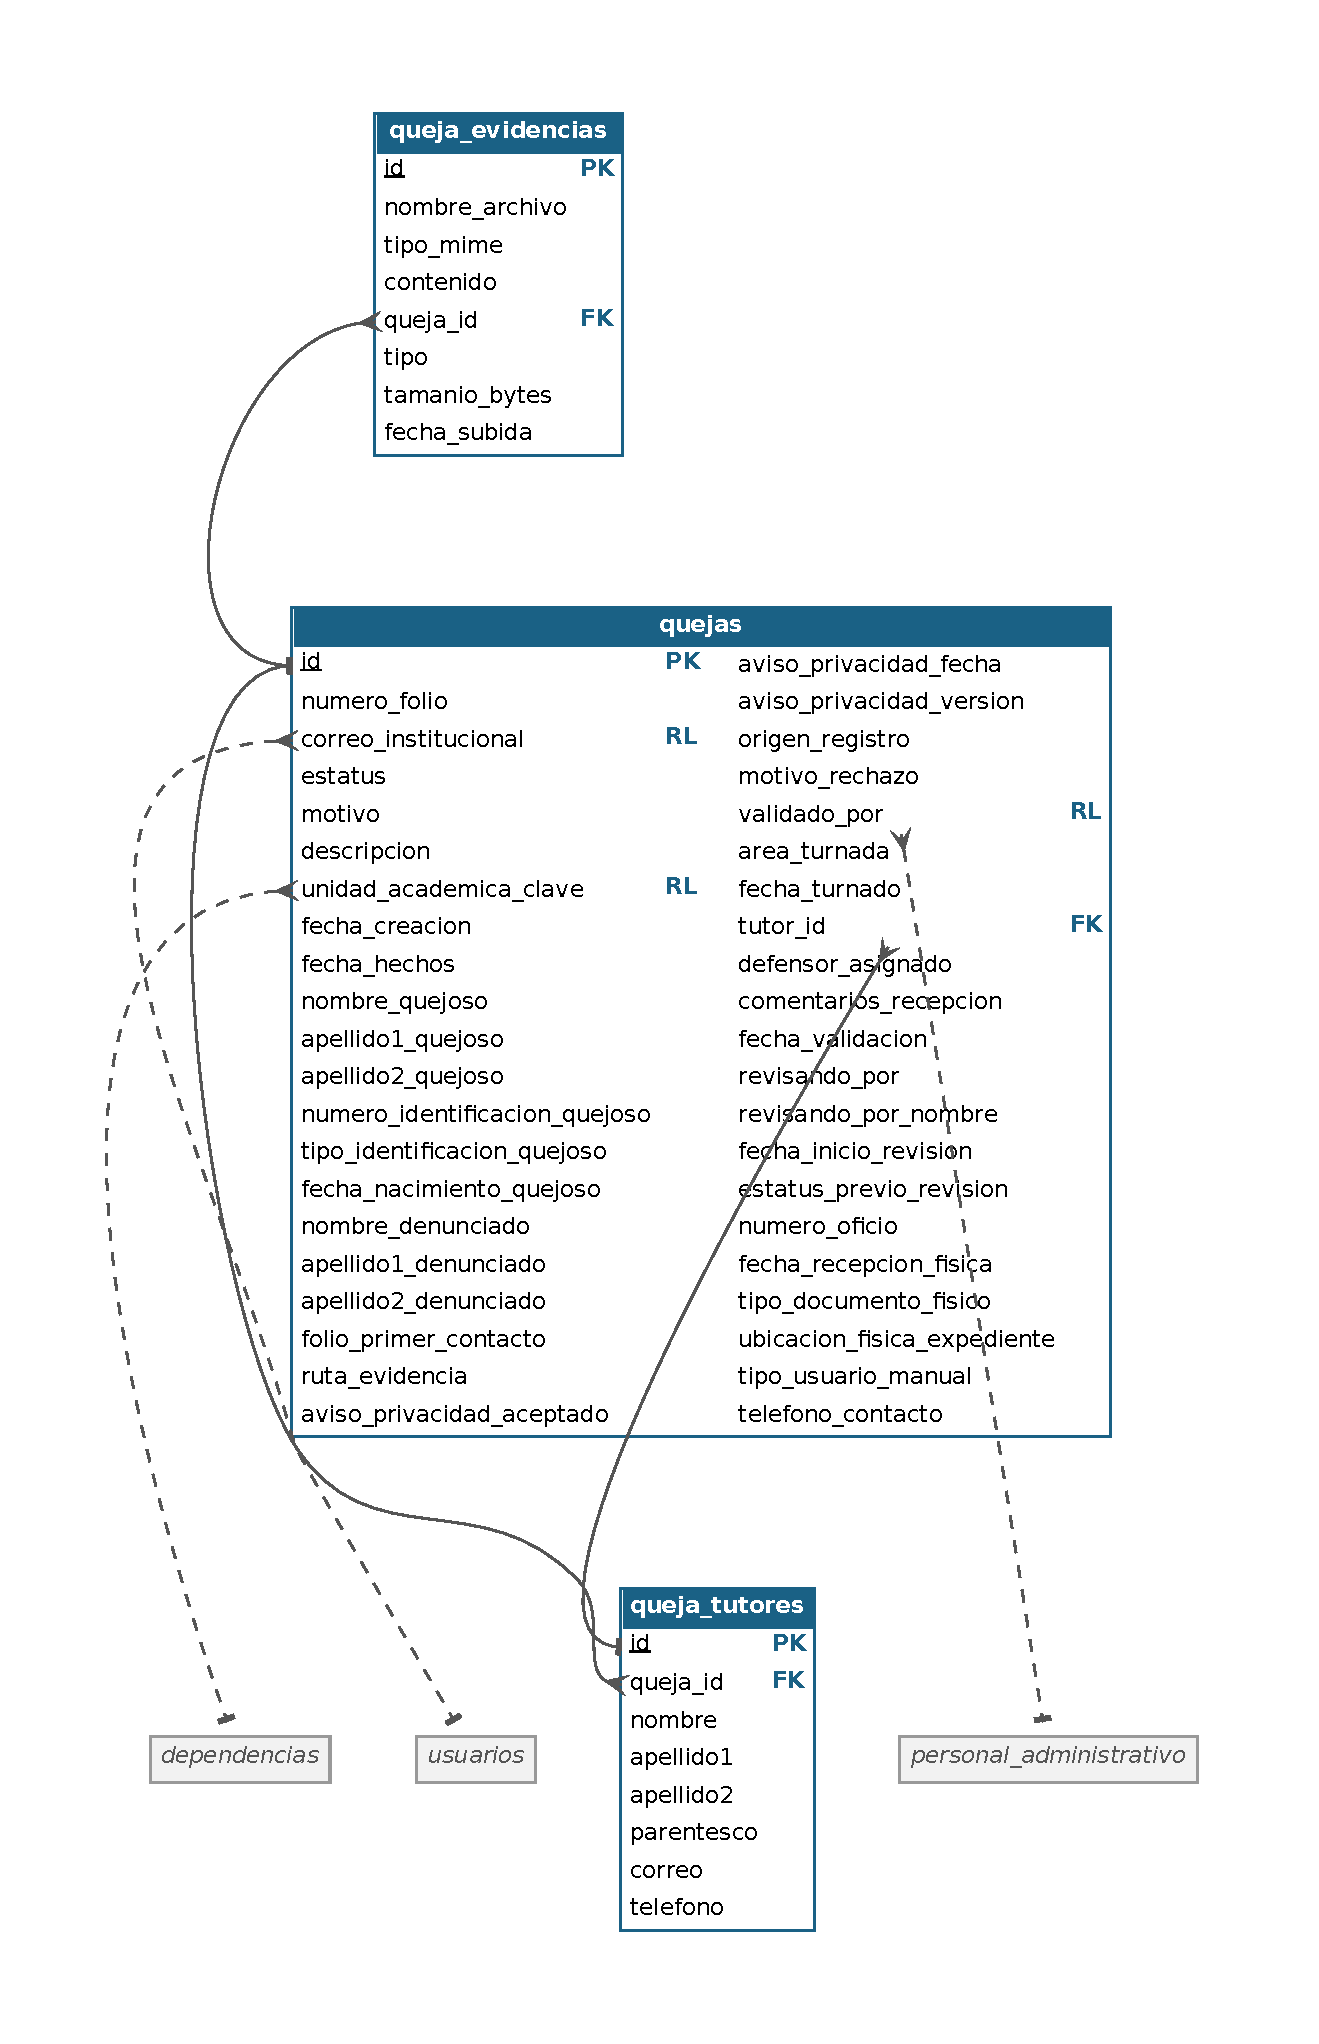
\includegraphics[width=\textwidth,height=0.85\textheight,keepaspectratio]{images/er_grupo_01.pdf}
	\caption{Diagrama entidad-relación: \texttt{quejas}, \texttt{queja\_tutores}, \texttt{queja\_evidencias}}
	\label{fig:er_grupo_01}
\end{figure}


\begin{figure}[H]
	\centering
	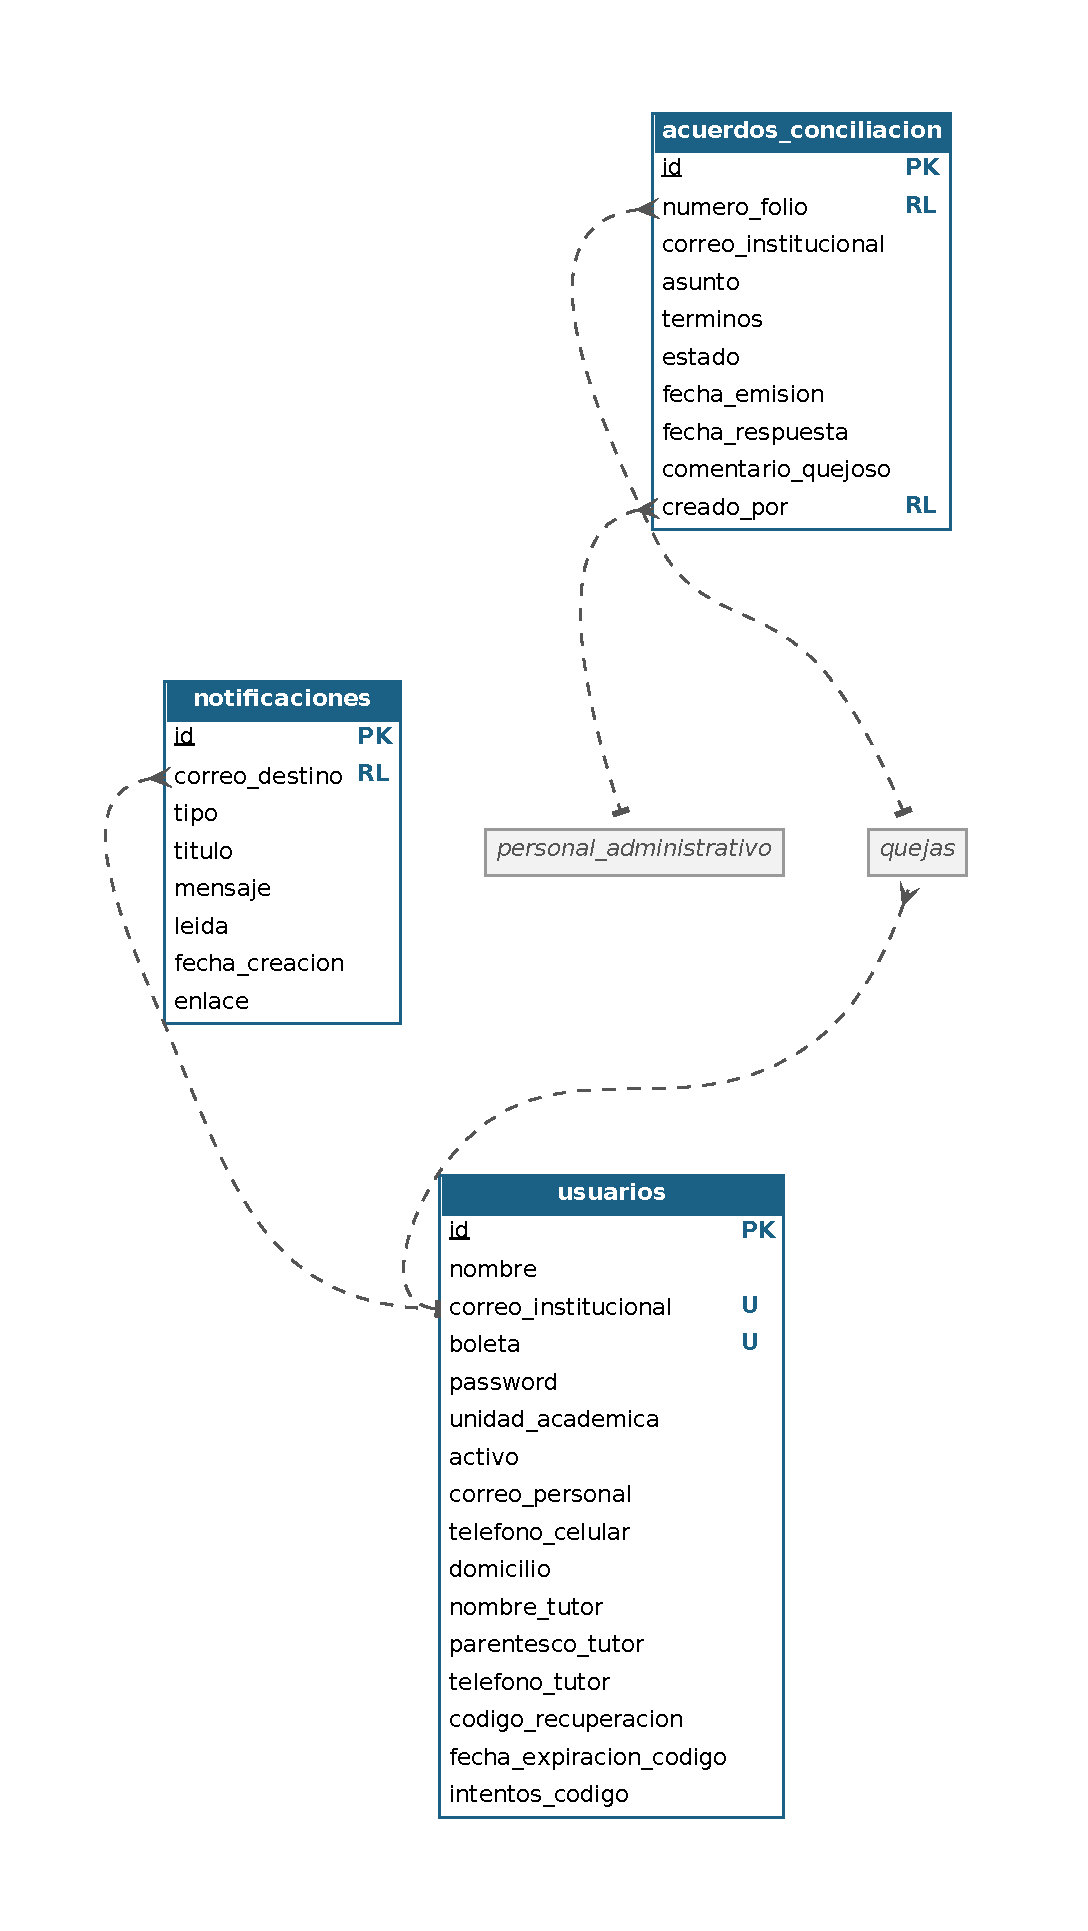
\includegraphics[width=\textwidth,height=0.85\textheight,keepaspectratio]{images/er_grupo_02.pdf}
	\caption{Diagrama entidad-relación: \texttt{usuarios}, \texttt{acuerdos\_conciliacion}, \texttt{notificaciones}}
	\label{fig:er_grupo_02}
\end{figure}

\subsection{Tabla \texttt{acuerdos\_conciliacion}}
Acuerdos de conciliación propuestos por la Defensoría y la respuesta del quejoso. Servicio responsable: revision-service, queja-service, primer-contacto-service.


\rowcolors{2}{rowblue}{white}
\footnotesize
\renewcommand{\arraystretch}{1.15}
\setlength{\tabcolsep}{4pt}
\begin{longtable}{|L{3.9cm}|L{2.4cm}|L{0.9cm}|L{1.2cm}|L{6.6cm}|}
	\hiderowcolors\caption{Diccionario de datos de la tabla \texttt{acuerdos\_conciliacion}}
	\label{tab:dic_acuerdos_conciliacion} \\ \showrowcolors
	\hline
	\rowcolor{headerblue}
	\headercell{Columna} & \headercell{Tipo} & \headercell{Nulo} & \headercell{Clave} & \headercell{Descripción} \\
	\hline
	\endfirsthead
	\hline
	\rowcolor{headerblue}
	\headercell{Columna} & \headercell{Tipo} & \headercell{Nulo} & \headercell{Clave} & \headercell{Descripción} \\
	\hline
	\endhead
		\texttt{id} & BIGINT & No & PK & Identificador único del registro, generado automáticamente. \\ \hline
		\texttt{numero\_\allowbreak{}folio} & VARCHAR(255) & No & RL & Folio de la queja a la que se dirige el acuerdo. \\ \hline
		\texttt{correo\_\allowbreak{}institucional} & VARCHAR(255) & No &  & Correo del quejoso destinatario; solo él puede responder. \\ \hline
		\texttt{asunto} & VARCHAR(255) & No &  & Asunto o tema del documento. \\ \hline
		\texttt{terminos} & TEXT & No &  & Términos del acuerdo. \\ \hline
		\texttt{estado} & VARCHAR(255) & No &  & Estado del acuerdo (pendiente, aceptado o rechazado). \\ \hline
		\texttt{fecha\_\allowbreak{}emision} & TIMESTAMP & Sí &  & Fecha y hora de emisión. \\ \hline
		\texttt{fecha\_\allowbreak{}respuesta} & TIMESTAMP & Sí &  & Fecha y hora de la respuesta. \\ \hline
		\texttt{comentario\_\allowbreak{}quejoso} & TEXT & Sí &  & Comentario del quejoso al responder. \\ \hline
		\texttt{creado\_\allowbreak{}por} & VARCHAR(255) & Sí & RL & Usuario que creó el registro. \\ \hline
\end{longtable}
\normalsize
\setlength{\tabcolsep}{6pt}
\renewcommand{\arraystretch}{1}

\subsection{Tabla \texttt{notificaciones}}
Avisos persistidos para cada destinatario, con su estado de lectura. Servicio responsable: notificaciones-service.


\rowcolors{2}{rowblue}{white}
\footnotesize
\renewcommand{\arraystretch}{1.15}
\setlength{\tabcolsep}{4pt}
\begin{longtable}{|L{3.9cm}|L{2.4cm}|L{0.9cm}|L{1.2cm}|L{6.6cm}|}
	\hiderowcolors\caption{Diccionario de datos de la tabla \texttt{notificaciones}}
	\label{tab:dic_notificaciones} \\ \showrowcolors
	\hline
	\rowcolor{headerblue}
	\headercell{Columna} & \headercell{Tipo} & \headercell{Nulo} & \headercell{Clave} & \headercell{Descripción} \\
	\hline
	\endfirsthead
	\hline
	\rowcolor{headerblue}
	\headercell{Columna} & \headercell{Tipo} & \headercell{Nulo} & \headercell{Clave} & \headercell{Descripción} \\
	\hline
	\endhead
		\texttt{id} & BIGINT & No & PK & Identificador único del registro, generado automáticamente. \\ \hline
		\texttt{correo\_\allowbreak{}destino} & VARCHAR(255) & No & RL & Correo electrónico del destinatario. \\ \hline
		\texttt{tipo} & VARCHAR(255) & No &  & Tipo de aviso. \\ \hline
		\texttt{titulo} & VARCHAR(255) & No &  & Título del aviso. \\ \hline
		\texttt{mensaje} & TEXT & Sí &  & Texto del aviso. \\ \hline
		\texttt{leida} & BOOLEAN & No &  & Indica si el aviso ya fue leído. \\ \hline
		\texttt{fecha\_\allowbreak{}creacion} & TIMESTAMP & Sí &  & Fecha y hora de creación del registro. \\ \hline
		\texttt{enlace} & VARCHAR(255) & Sí &  & Enlace de la plataforma relacionado con el aviso. \\ \hline
\end{longtable}
\normalsize
\setlength{\tabcolsep}{6pt}
\renewcommand{\arraystretch}{1}

\subsection{Tabla \texttt{queja\_evidencias}}
Archivos de evidencia adjuntos a una queja, almacenados con su contenido binario. Servicio responsable: queja-service.


\rowcolors{2}{rowblue}{white}
\footnotesize
\renewcommand{\arraystretch}{1.15}
\setlength{\tabcolsep}{4pt}
\begin{longtable}{|L{3.9cm}|L{2.4cm}|L{0.9cm}|L{1.2cm}|L{6.6cm}|}
	\hiderowcolors\caption{Diccionario de datos de la tabla \texttt{queja\_evidencias}}
	\label{tab:dic_queja_evidencias} \\ \showrowcolors
	\hline
	\rowcolor{headerblue}
	\headercell{Columna} & \headercell{Tipo} & \headercell{Nulo} & \headercell{Clave} & \headercell{Descripción} \\
	\hline
	\endfirsthead
	\hline
	\rowcolor{headerblue}
	\headercell{Columna} & \headercell{Tipo} & \headercell{Nulo} & \headercell{Clave} & \headercell{Descripción} \\
	\hline
	\endhead
		\texttt{id} & BIGINT & No & PK & Identificador único del registro, generado automáticamente. \\ \hline
		\texttt{nombre\_\allowbreak{}archivo} & VARCHAR(255) & No &  & Nombre original del archivo. \\ \hline
		\texttt{tipo\_\allowbreak{}mime} & VARCHAR(255) & Sí &  & Tipo MIME del archivo. \\ \hline
		\texttt{contenido} & BYTEA & No &  & Contenido binario del archivo. \\ \hline
		\texttt{queja\_\allowbreak{}id} & BIGINT & No & FK & Queja a la que pertenece el registro. \\ \hline
		\texttt{tipo} & VARCHAR(20) & Sí &  & Clasificación del archivo (evidencia o identificación). \\ \hline
		\texttt{tamanio\_\allowbreak{}bytes} & BIGINT & Sí &  & Tamaño del archivo en bytes. \\ \hline
		\texttt{fecha\_\allowbreak{}subida} & TIMESTAMP & Sí &  & Fecha y hora en que se subió el archivo. \\ \hline
\end{longtable}
\normalsize
\setlength{\tabcolsep}{6pt}
\renewcommand{\arraystretch}{1}

\subsection{Tabla \texttt{queja\_tutores}}
Datos del tutor o adulto responsable cuando el quejoso es menor de edad; relación uno a uno con la queja. Servicio responsable: queja-service.


\rowcolors{2}{rowblue}{white}
\footnotesize
\renewcommand{\arraystretch}{1.15}
\setlength{\tabcolsep}{4pt}
\begin{longtable}{|L{3.9cm}|L{2.4cm}|L{0.9cm}|L{1.2cm}|L{6.6cm}|}
	\hiderowcolors\caption{Diccionario de datos de la tabla \texttt{queja\_tutores}}
	\label{tab:dic_queja_tutores} \\ \showrowcolors
	\hline
	\rowcolor{headerblue}
	\headercell{Columna} & \headercell{Tipo} & \headercell{Nulo} & \headercell{Clave} & \headercell{Descripción} \\
	\hline
	\endfirsthead
	\hline
	\rowcolor{headerblue}
	\headercell{Columna} & \headercell{Tipo} & \headercell{Nulo} & \headercell{Clave} & \headercell{Descripción} \\
	\hline
	\endhead
		\texttt{id} & BIGINT & No & PK & Identificador único del registro, generado automáticamente. \\ \hline
		\texttt{queja\_\allowbreak{}id} & BIGINT & No & FK & Queja a la que pertenece el registro. \\ \hline
		\texttt{nombre} & VARCHAR(255) & Sí &  & Nombre del tutor. \\ \hline
		\texttt{apellido1} & VARCHAR(255) & Sí &  & Primer apellido. \\ \hline
		\texttt{apellido2} & VARCHAR(255) & Sí &  & Segundo apellido. \\ \hline
		\texttt{parentesco} & VARCHAR(255) & Sí &  & Parentesco con el quejoso. \\ \hline
		\texttt{correo} & VARCHAR(255) & Sí &  & Correo del tutor. \\ \hline
		\texttt{telefono} & VARCHAR(255) & Sí &  & Teléfono del tutor. \\ \hline
\end{longtable}
\normalsize
\setlength{\tabcolsep}{6pt}
\renewcommand{\arraystretch}{1}

\subsection{Tabla \texttt{quejas}}
Registro central de cada queja: folio, identidad del quejoso, narrativa de los hechos, persona señalada, estatus y datos del flujo de recepción (validación, rechazo y turnado). Es la tabla de la que parte todo el expediente. Servicio responsable: queja-service, revision-service, primer-contacto-service, subdefensoria-service.


\rowcolors{2}{rowblue}{white}
\footnotesize
\renewcommand{\arraystretch}{1.15}
\setlength{\tabcolsep}{4pt}
\begin{longtable}{|L{3.9cm}|L{2.4cm}|L{0.9cm}|L{1.2cm}|L{6.6cm}|}
	\hiderowcolors\caption{Diccionario de datos de la tabla \texttt{quejas}}
	\label{tab:dic_quejas} \\ \showrowcolors
	\hline
	\rowcolor{headerblue}
	\headercell{Columna} & \headercell{Tipo} & \headercell{Nulo} & \headercell{Clave} & \headercell{Descripción} \\
	\hline
	\endfirsthead
	\hline
	\rowcolor{headerblue}
	\headercell{Columna} & \headercell{Tipo} & \headercell{Nulo} & \headercell{Clave} & \headercell{Descripción} \\
	\hline
	\endhead
		\texttt{id} & BIGINT & No & PK & Identificador único del registro, generado automáticamente. \\ \hline
		\texttt{numero\_\allowbreak{}folio} & VARCHAR(255) & No &  & Folio de seguimiento que se entrega al quejoso. \\ \hline
		\texttt{correo\_\allowbreak{}institucional} & VARCHAR(255) & No & RL & Correo del quejoso; junto con el folio permite consultar la queja y activar la cuenta. \\ \hline
		\texttt{estatus} & VARCHAR(255) & Sí &  & Estatus de la queja (RECIBIDA, EN\_VALIDACION, RECHAZADA, TURNADA, entre otros). \\ \hline
		\texttt{motivo} & VARCHAR(255) & No &  & Motivo de la queja. \\ \hline
		\texttt{descripcion} & TEXT & Sí &  & Narrativa de los hechos redactada por el quejoso. \\ \hline
		\texttt{unidad\_\allowbreak{}academica\_\allowbreak{}clave} & VARCHAR(255) & Sí & RL & Clave de la unidad académica involucrada, tomada del catálogo. \\ \hline
		\texttt{fecha\_\allowbreak{}creacion} & TIMESTAMP & Sí &  & Fecha y hora en que se registró la queja. \\ \hline
		\texttt{fecha\_\allowbreak{}hechos} & DATE & Sí &  & Fecha en que ocurrieron los hechos. \\ \hline
		\texttt{nombre\_\allowbreak{}quejoso} & VARCHAR(255) & Sí &  & Nombre del quejoso. \\ \hline
		\texttt{apellido1\_\allowbreak{}quejoso} & VARCHAR(255) & Sí &  & Primer apellido del quejoso. \\ \hline
		\texttt{apellido2\_\allowbreak{}quejoso} & VARCHAR(255) & Sí &  & Segundo apellido del quejoso. \\ \hline
		\texttt{numero\_\allowbreak{}identificacion\_\allowbreak{}quejoso} & VARCHAR(255) & Sí &  & Número de boleta o de empleado del quejoso. \\ \hline
		\texttt{tipo\_\allowbreak{}identificacion\_\allowbreak{}quejoso} & VARCHAR(255) & Sí &  & Tipo de identificación del quejoso. \\ \hline
		\texttt{fecha\_\allowbreak{}nacimiento\_\allowbreak{}quejoso} & DATE & Sí &  & Fecha de nacimiento del quejoso, usada para identificar a menores de edad. \\ \hline
		\texttt{nombre\_\allowbreak{}denunciado} & VARCHAR(255) & Sí &  & Nombre de la persona señalada. \\ \hline
		\texttt{apellido1\_\allowbreak{}denunciado} & VARCHAR(255) & Sí &  & Primer apellido de la persona señalada. \\ \hline
		\texttt{apellido2\_\allowbreak{}denunciado} & VARCHAR(255) & Sí &  & Segundo apellido de la persona señalada. \\ \hline
		\texttt{folio\_\allowbreak{}primer\_\allowbreak{}contacto} & VARCHAR(255) & Sí &  & Folio asignado en Primer Contacto. \\ \hline
		\texttt{ruta\_\allowbreak{}evidencia} & VARCHAR(255) & Sí &  & Ruta de la evidencia principal de la queja. \\ \hline
		\texttt{aviso\_\allowbreak{}privacidad\_\allowbreak{}aceptado} & BOOLEAN & Sí &  & Indica si se aceptó el aviso de privacidad. \\ \hline
		\texttt{aviso\_\allowbreak{}privacidad\_\allowbreak{}fecha} & TIMESTAMP & Sí &  & Fecha y hora de aceptación del aviso de privacidad. \\ \hline
		\texttt{aviso\_\allowbreak{}privacidad\_\allowbreak{}version} & VARCHAR(255) & Sí &  & Versión del aviso de privacidad aceptada. \\ \hline
		\texttt{origen\_\allowbreak{}registro} & VARCHAR(255) & Sí &  & Punto de acceso por el que ingresó la queja (público, autenticado o manual). \\ \hline
		\texttt{motivo\_\allowbreak{}rechazo} & TEXT & Sí &  & Motivos y observaciones del rechazo. \\ \hline
		\texttt{validado\_\allowbreak{}por} & VARCHAR(255) & Sí & RL & Correo de la persona de Recepción que validó la queja. \\ \hline
		\texttt{area\_\allowbreak{}turnada} & VARCHAR(255) & Sí &  & Área a la que Recepción turnó la queja. \\ \hline
		\texttt{fecha\_\allowbreak{}turnado} & TIMESTAMP & Sí &  & Fecha y hora del turnado. \\ \hline
		\texttt{tutor\_\allowbreak{}id} & BIGINT & Sí & FK & Tutor asociado a la queja, cuando el quejoso es menor de edad. \\ \hline
		\texttt{defensor\_\allowbreak{}asignado} & VARCHAR(255) & Sí &  & Defensor o analista al que se asignó la queja al turnarla. \\ \hline
		\texttt{comentarios\_\allowbreak{}recepcion} & TEXT & Sí &  & Comentarios de Recepción al turnar la queja. \\ \hline
		\texttt{fecha\_\allowbreak{}validacion} & TIMESTAMP & Sí &  & Fecha y hora de la validación por Recepción. \\ \hline
		\texttt{revisando\_\allowbreak{}por} & VARCHAR(255) & Sí &  & Correo de la persona de Recepción que tiene tomada la queja. \\ \hline
		\texttt{revisando\_\allowbreak{}por\_\allowbreak{}nombre} & VARCHAR(255) & Sí &  & Nombre de la persona de Recepción que tiene tomada la queja. \\ \hline
		\texttt{fecha\_\allowbreak{}inicio\_\allowbreak{}revision} & TIMESTAMP & Sí &  & Fecha y hora en que Recepción tomó la queja para revisarla. \\ \hline
		\texttt{estatus\_\allowbreak{}previo\_\allowbreak{}revision} & VARCHAR(255) & Sí &  & Estatus que tenía la queja antes de que Recepción la tomara. \\ \hline
		\texttt{numero\_\allowbreak{}oficio} & VARCHAR(255) & Sí &  & Número del oficio. \\ \hline
		\texttt{fecha\_\allowbreak{}recepcion\_\allowbreak{}fisica} & DATE & Sí &  & Fecha de recepción del documento físico. \\ \hline
		\texttt{tipo\_\allowbreak{}documento\_\allowbreak{}fisico} & VARCHAR(255) & Sí &  & Tipo del documento físico recibido. \\ \hline
		\texttt{ubicacion\_\allowbreak{}fisica\_\allowbreak{}expediente} & VARCHAR(255) & Sí &  & Ubicación física del expediente en papel. \\ \hline
		\texttt{tipo\_\allowbreak{}usuario\_\allowbreak{}manual} & VARCHAR(255) & Sí &  & Tipo de usuario capturado en el registro manual. \\ \hline
		\texttt{telefono\_\allowbreak{}contacto} & VARCHAR(255) & Sí &  & Teléfono de contacto del quejoso. \\ \hline
\end{longtable}
\normalsize
\setlength{\tabcolsep}{6pt}
\renewcommand{\arraystretch}{1}

\subsection{Tabla \texttt{usuarios}}
Cuentas de seguimiento de los quejosos: identidad institucional, credencial cifrada, datos de contacto y código de recuperación. Servicio responsable: auth-service, queja-service.


\rowcolors{2}{rowblue}{white}
\footnotesize
\renewcommand{\arraystretch}{1.15}
\setlength{\tabcolsep}{4pt}
\begin{longtable}{|L{3.9cm}|L{2.4cm}|L{0.9cm}|L{1.2cm}|L{6.6cm}|}
	\hiderowcolors\caption{Diccionario de datos de la tabla \texttt{usuarios}}
	\label{tab:dic_usuarios} \\ \showrowcolors
	\hline
	\rowcolor{headerblue}
	\headercell{Columna} & \headercell{Tipo} & \headercell{Nulo} & \headercell{Clave} & \headercell{Descripción} \\
	\hline
	\endfirsthead
	\hline
	\rowcolor{headerblue}
	\headercell{Columna} & \headercell{Tipo} & \headercell{Nulo} & \headercell{Clave} & \headercell{Descripción} \\
	\hline
	\endhead
		\texttt{id} & BIGINT & No & PK & Identificador único del registro, generado automáticamente. \\ \hline
		\texttt{nombre} & VARCHAR(255) & No &  & Nombre completo del quejoso. \\ \hline
		\texttt{correo\_\allowbreak{}institucional} & VARCHAR(255) & No & U & Correo institucional del titular del registro. \\ \hline
		\texttt{boleta} & VARCHAR(255) & No & U & Número de boleta o de empleado del usuario. \\ \hline
		\texttt{password} & VARCHAR(255) & Sí &  & Contraseña cifrada mediante función de resumen. \\ \hline
		\texttt{unidad\_\allowbreak{}academica} & VARCHAR(255) & Sí &  & Unidad académica del quejoso. \\ \hline
		\texttt{activo} & BOOLEAN & Sí &  & Indica si la cuenta está activada. \\ \hline
		\texttt{correo\_\allowbreak{}personal} & VARCHAR(255) & Sí &  & Correo personal del quejoso. \\ \hline
		\texttt{telefono\_\allowbreak{}celular} & VARCHAR(255) & Sí &  & Teléfono celular del quejoso. \\ \hline
		\texttt{domicilio} & TEXT & Sí &  & Domicilio del quejoso. \\ \hline
		\texttt{nombre\_\allowbreak{}tutor} & VARCHAR(255) & Sí &  & Nombre del tutor del quejoso. \\ \hline
		\texttt{parentesco\_\allowbreak{}tutor} & VARCHAR(255) & Sí &  & Parentesco del tutor con el quejoso. \\ \hline
		\texttt{telefono\_\allowbreak{}tutor} & VARCHAR(255) & Sí &  & Teléfono del tutor. \\ \hline
		\texttt{codigo\_\allowbreak{}recuperacion} & VARCHAR(255) & Sí &  & Código de seis dígitos para restablecer la contraseña. \\ \hline
		\texttt{fecha\_\allowbreak{}expiracion\_\allowbreak{}codigo} & TIMESTAMP & Sí &  & Fecha y hora de expiración del código de recuperación. \\ \hline
		\texttt{intentos\_\allowbreak{}codigo} & INTEGER & Sí &  & Número de intentos fallidos con el código de recuperación. \\ \hline
\end{longtable}
\normalsize
\setlength{\tabcolsep}{6pt}
\renewcommand{\arraystretch}{1}

\section{Módulo: Primer Contacto}
\label{anx:bd_mod2}

Las figuras de esta sección muestran el diagrama entidad-relación del módulo con todas sus columnas, divididas en grupos de tablas para facilitar su lectura. Las tablas en gris pertenecen a otros grupos o módulos y se incluyen solo para mostrar las relaciones.


\begin{figure}[H]
	\centering
	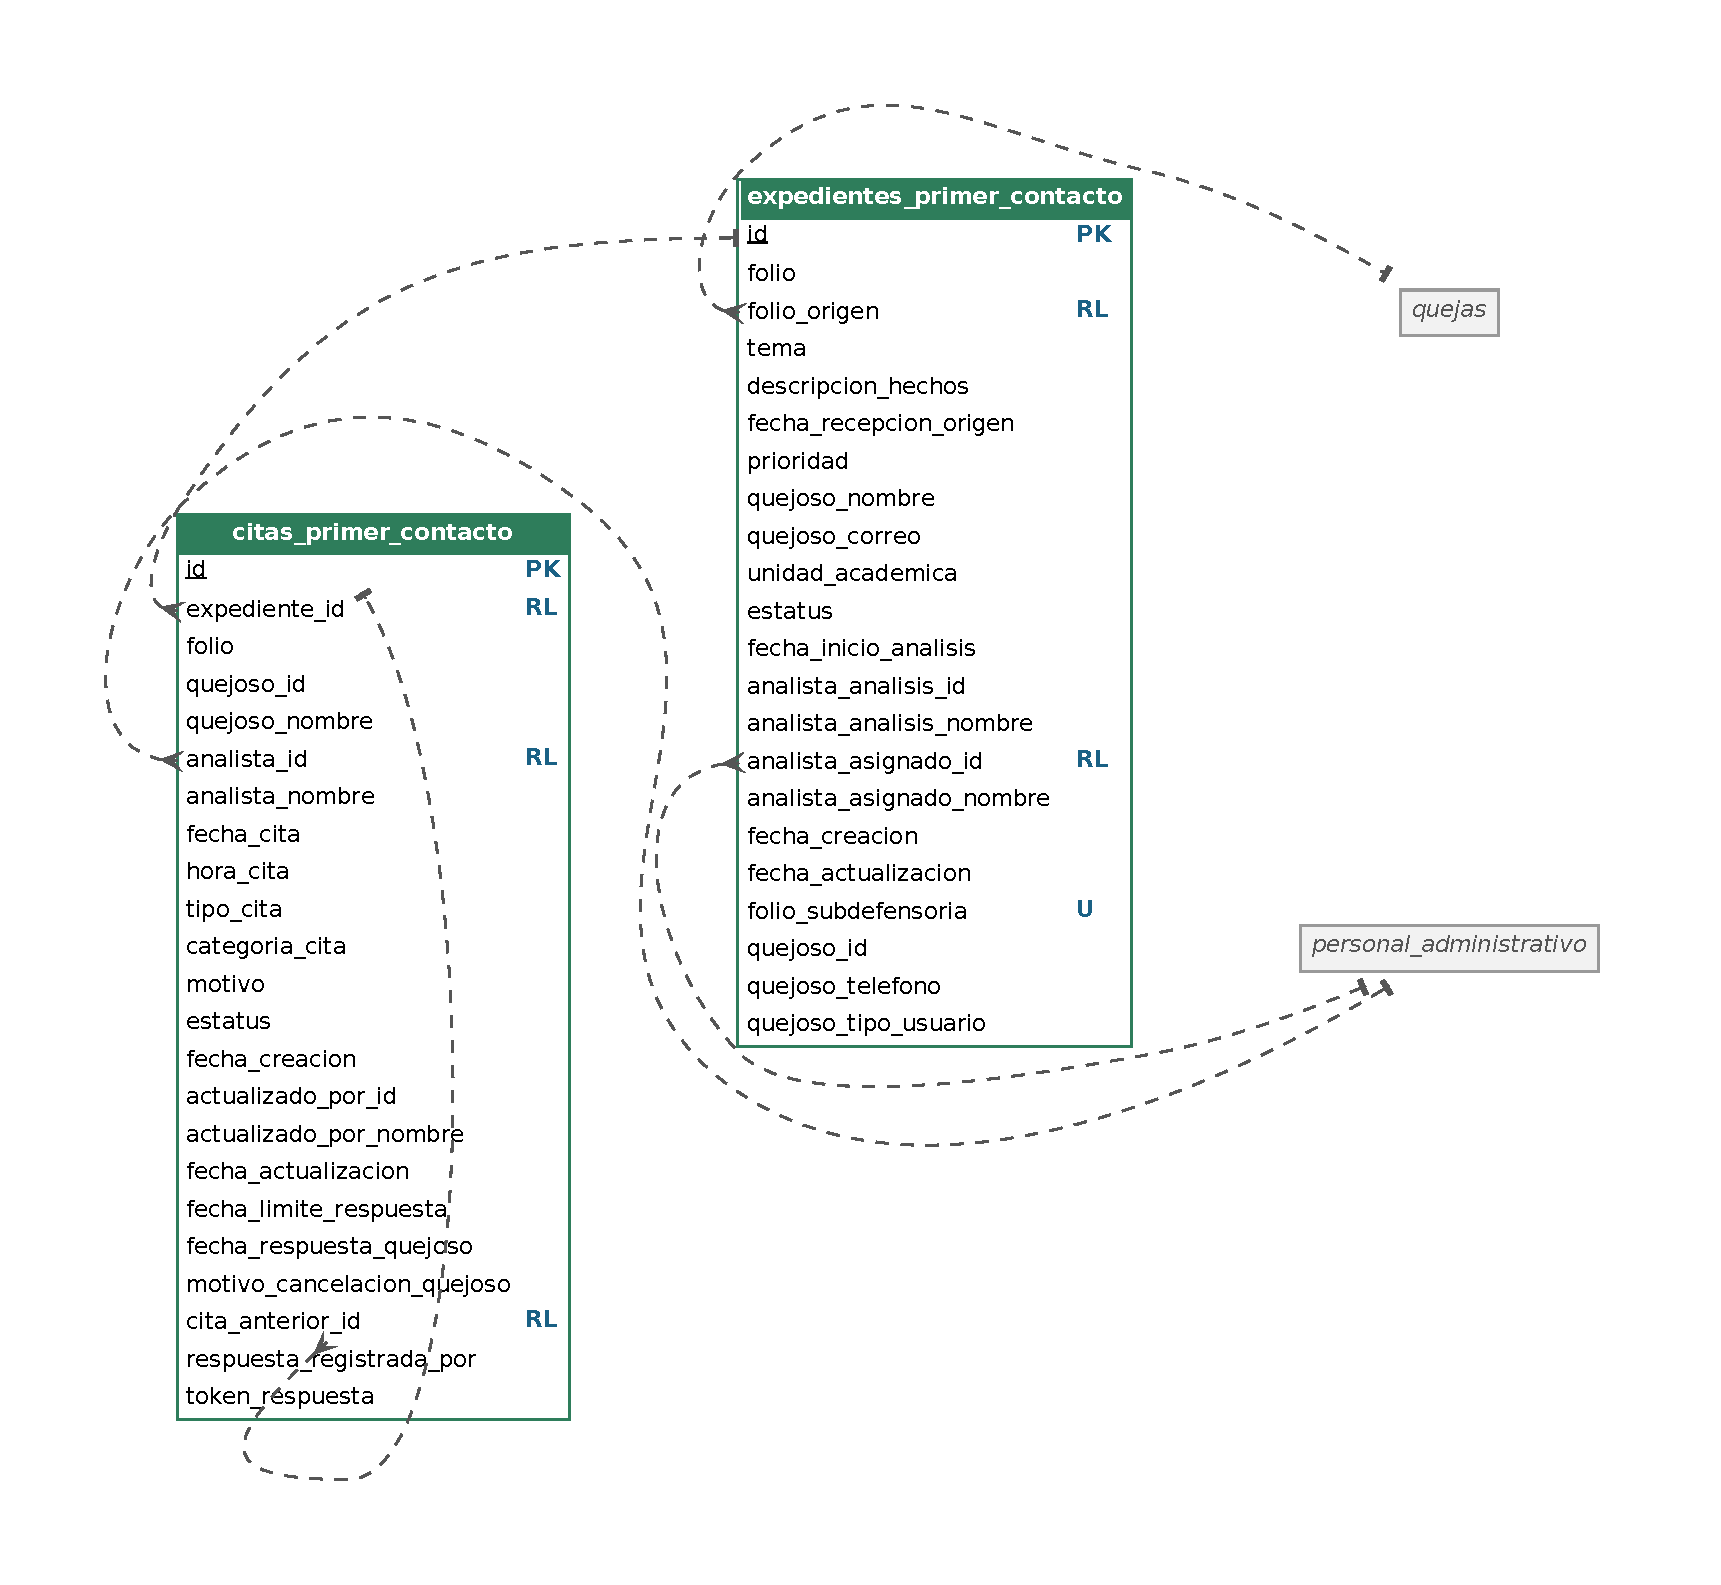
\includegraphics[width=\textwidth,height=0.85\textheight,keepaspectratio]{images/er_grupo_03.pdf}
	\caption{Diagrama entidad-relación: \texttt{expedientes\_primer\_contacto}, \texttt{citas\_primer\_contacto}}
	\label{fig:er_grupo_03}
\end{figure}


\begin{figure}[H]
	\centering
	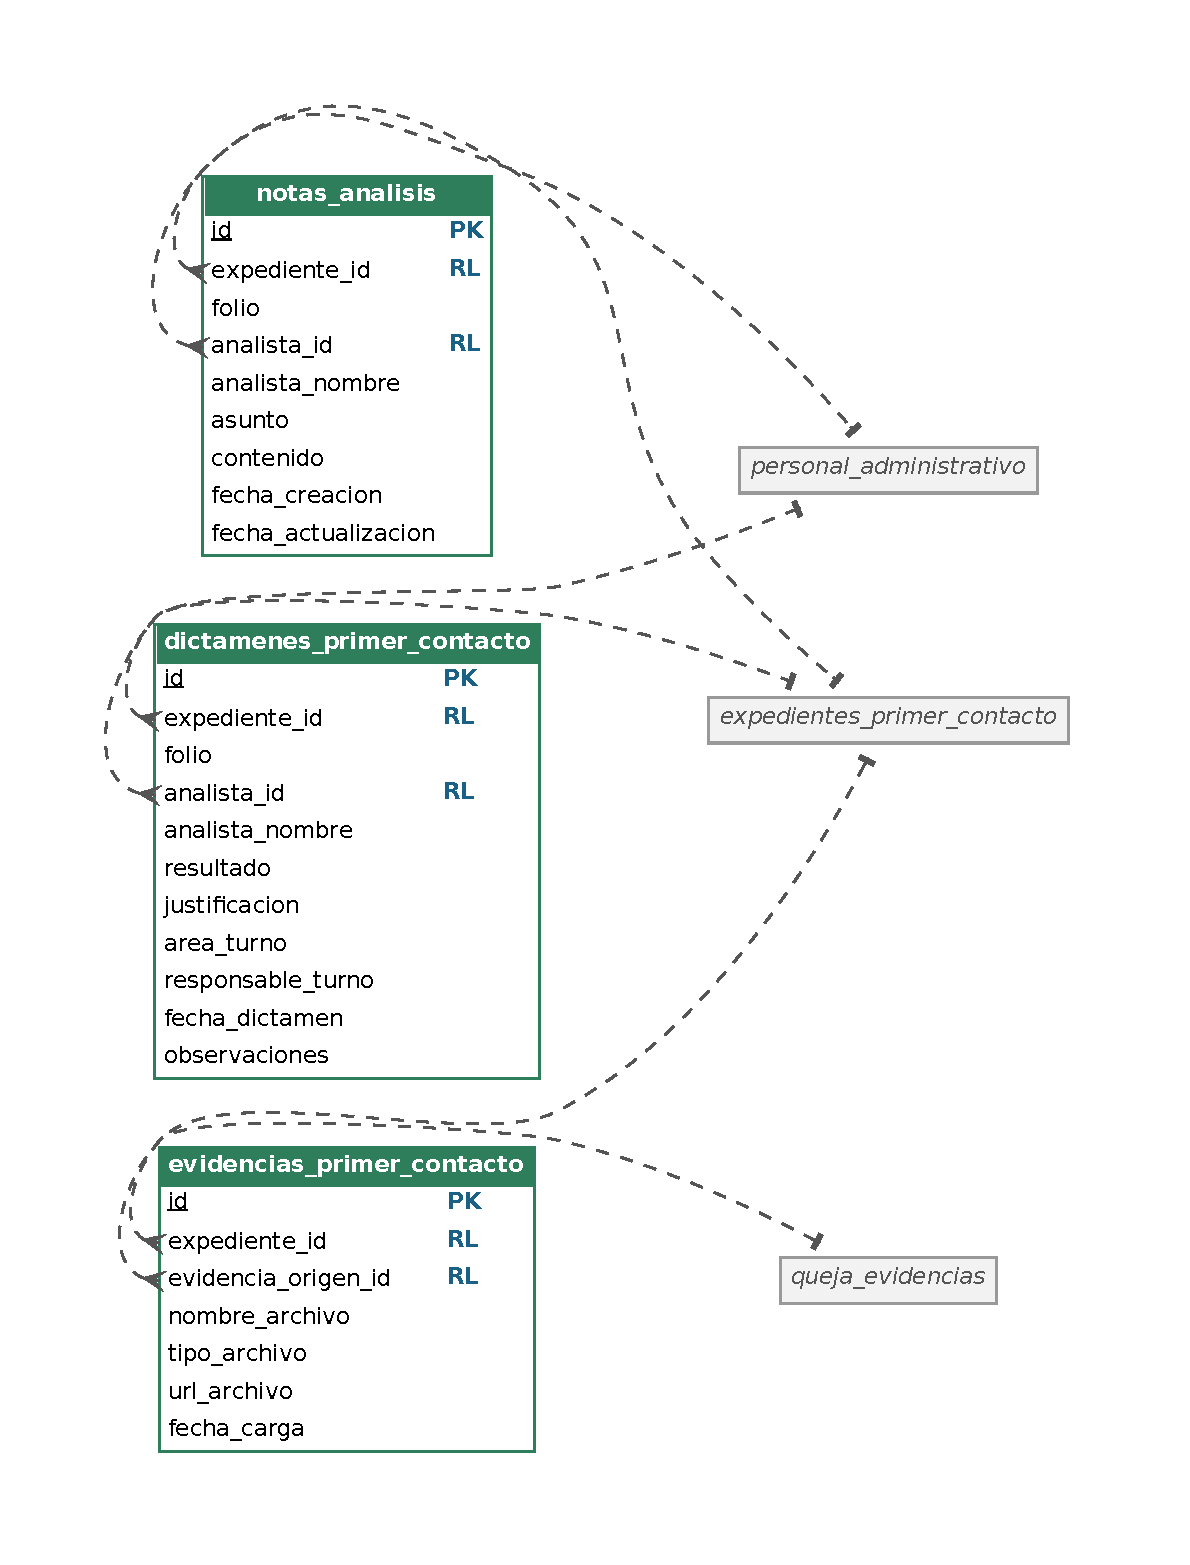
\includegraphics[width=\textwidth,height=0.85\textheight,keepaspectratio]{images/er_grupo_04.pdf}
	\caption{Diagrama entidad-relación: \texttt{dictamenes\_primer\_contacto}, \texttt{notas\_analisis}, \texttt{evidencias\_primer\_contacto}}
	\label{fig:er_grupo_04}
\end{figure}


\begin{figure}[H]
	\centering
	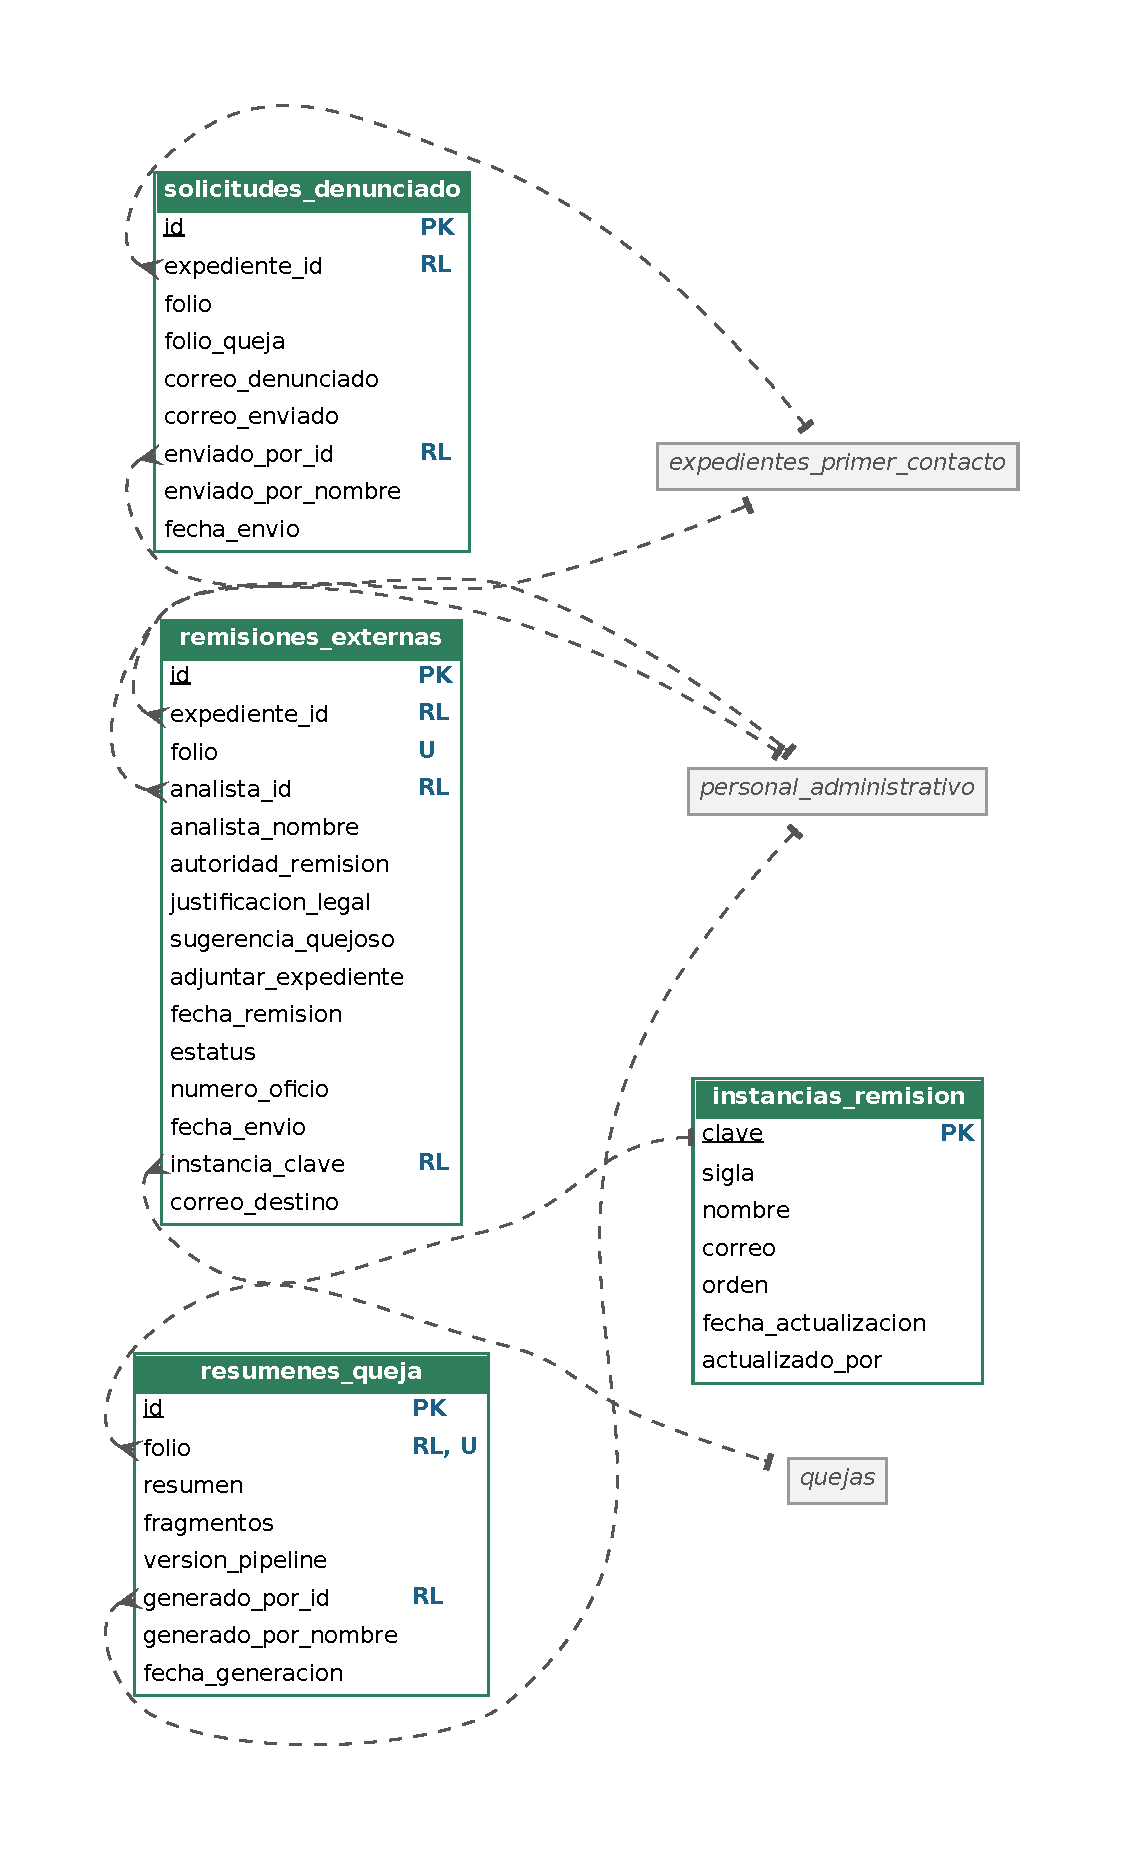
\includegraphics[width=\textwidth,height=0.85\textheight,keepaspectratio]{images/er_grupo_05.pdf}
	\caption{Diagrama entidad-relación: \texttt{remisiones\_externas}, \texttt{instancias\_remision}, \texttt{solicitudes\_denunciado}, \texttt{resumenes\_queja}}
	\label{fig:er_grupo_05}
\end{figure}


\begin{figure}[H]
	\centering
	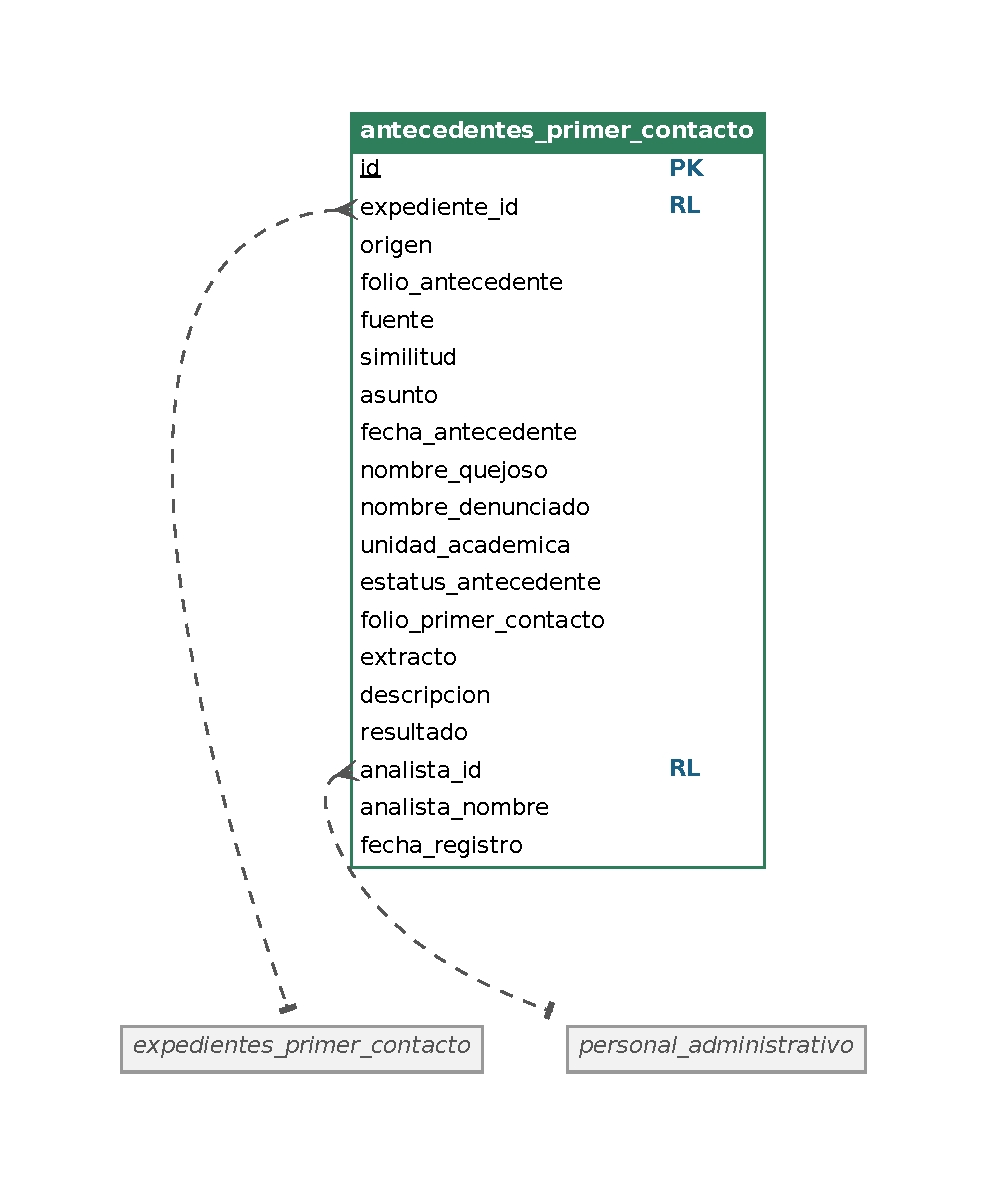
\includegraphics[width=\textwidth,height=0.85\textheight,keepaspectratio]{images/er_grupo_06.pdf}
	\caption{Diagrama entidad-relación: \texttt{antecedentes\_primer\_contacto}}
	\label{fig:er_grupo_06}
\end{figure}

\subsection{Tabla \texttt{antecedentes\_primer\_contacto}}
Antecedentes vinculados a un expediente, ya sea sugeridos por el modelo de búsqueda o agregados manualmente, con la decisión del analista. Servicio responsable: primer-contacto-service.


\rowcolors{2}{rowblue}{white}
\footnotesize
\renewcommand{\arraystretch}{1.15}
\setlength{\tabcolsep}{4pt}
\begin{longtable}{|L{3.9cm}|L{2.4cm}|L{0.9cm}|L{1.2cm}|L{6.6cm}|}
	\hiderowcolors\caption{Diccionario de datos de la tabla \texttt{antecedentes\_primer\_contacto}}
	\label{tab:dic_antecedentes_primer_contacto} \\ \showrowcolors
	\hline
	\rowcolor{headerblue}
	\headercell{Columna} & \headercell{Tipo} & \headercell{Nulo} & \headercell{Clave} & \headercell{Descripción} \\
	\hline
	\endfirsthead
	\hline
	\rowcolor{headerblue}
	\headercell{Columna} & \headercell{Tipo} & \headercell{Nulo} & \headercell{Clave} & \headercell{Descripción} \\
	\hline
	\endhead
		\texttt{id} & BIGINT & No & PK & Identificador único del registro, generado automáticamente. \\ \hline
		\texttt{expediente\_\allowbreak{}id} & BIGINT & No & RL & Expediente al que pertenece el registro. \\ \hline
		\texttt{origen} & VARCHAR(20) & No &  & Cómo se vinculó el antecedente (sugerido por el modelo o agregado manualmente). \\ \hline
		\texttt{folio\_\allowbreak{}antecedente} & VARCHAR(60) & No &  & Folio del expediente antecedente. \\ \hline
		\texttt{fuente} & VARCHAR(30) & No &  & Fuente del antecedente (base vigente o histórica). \\ \hline
		\texttt{similitud} & INTEGER & Sí &  & Porcentaje de similitud reportado por el modelo de antecedentes. \\ \hline
		\texttt{asunto} & VARCHAR(500) & Sí &  & Asunto o tema del documento. \\ \hline
		\texttt{fecha\_\allowbreak{}antecedente} & VARCHAR(30) & Sí &  & Fecha del expediente antecedente. \\ \hline
		\texttt{nombre\_\allowbreak{}quejoso} & VARCHAR(300) & Sí &  & Nombre del quejoso. \\ \hline
		\texttt{nombre\_\allowbreak{}denunciado} & VARCHAR(300) & Sí &  & Nombre de la persona señalada. \\ \hline
		\texttt{unidad\_\allowbreak{}academica} & VARCHAR(60) & Sí &  & Unidad académica relacionada. \\ \hline
		\texttt{estatus\_\allowbreak{}antecedente} & VARCHAR(50) & Sí &  & Estatus del expediente antecedente al momento de vincularlo. \\ \hline
		\texttt{folio\_\allowbreak{}primer\_\allowbreak{}contacto} & VARCHAR(50) & Sí &  & Folio asignado en Primer Contacto. \\ \hline
		\texttt{extracto} & TEXT & Sí &  & Fragmento del antecedente que coincide con la queja. \\ \hline
		\texttt{descripcion} & TEXT & Sí &  & Narrativa del expediente antecedente. \\ \hline
		\texttt{resultado} & VARCHAR(50) & Sí &  & Decisión del analista sobre el antecedente. \\ \hline
		\texttt{analista\_\allowbreak{}id} & BIGINT & No & RL & Identificador del analista que registró el elemento. \\ \hline
		\texttt{analista\_\allowbreak{}nombre} & VARCHAR(150) & Sí &  & Nombre del analista que registró el elemento. \\ \hline
		\texttt{fecha\_\allowbreak{}registro} & TIMESTAMP & No &  & Fecha y hora del registro. \\ \hline
\end{longtable}
\normalsize
\setlength{\tabcolsep}{6pt}
\renewcommand{\arraystretch}{1}

\subsection{Tabla \texttt{citas\_primer\_contacto}}
Citas programadas con el quejoso o con la persona señalada durante el análisis, con su estado y la respuesta de la persona citada. Servicio responsable: primer-contacto-service.


\rowcolors{2}{rowblue}{white}
\footnotesize
\renewcommand{\arraystretch}{1.15}
\setlength{\tabcolsep}{4pt}
\begin{longtable}{|L{3.9cm}|L{2.4cm}|L{0.9cm}|L{1.2cm}|L{6.6cm}|}
	\hiderowcolors\caption{Diccionario de datos de la tabla \texttt{citas\_primer\_contacto}}
	\label{tab:dic_citas_primer_contacto} \\ \showrowcolors
	\hline
	\rowcolor{headerblue}
	\headercell{Columna} & \headercell{Tipo} & \headercell{Nulo} & \headercell{Clave} & \headercell{Descripción} \\
	\hline
	\endfirsthead
	\hline
	\rowcolor{headerblue}
	\headercell{Columna} & \headercell{Tipo} & \headercell{Nulo} & \headercell{Clave} & \headercell{Descripción} \\
	\hline
	\endhead
		\texttt{id} & BIGINT & No & PK & Identificador único del registro, generado automáticamente. \\ \hline
		\texttt{expediente\_\allowbreak{}id} & BIGINT & No & RL & Expediente al que pertenece el registro. \\ \hline
		\texttt{folio} & VARCHAR(50) & No &  & Folio del expediente de Primer Contacto. \\ \hline
		\texttt{quejoso\_\allowbreak{}id} & BIGINT & Sí &  & Identificador de la cuenta del quejoso, si existe. \\ \hline
		\texttt{quejoso\_\allowbreak{}nombre} & VARCHAR(150) & Sí &  & Nombre del quejoso. \\ \hline
		\texttt{analista\_\allowbreak{}id} & BIGINT & No & RL & Identificador del analista que registró el elemento. \\ \hline
		\texttt{analista\_\allowbreak{}nombre} & VARCHAR(150) & Sí &  & Nombre del analista que registró el elemento. \\ \hline
		\texttt{fecha\_\allowbreak{}cita} & DATE & No &  & Fecha de la cita. \\ \hline
		\texttt{hora\_\allowbreak{}cita} & TIME & No &  & Hora de la cita. \\ \hline
		\texttt{tipo\_\allowbreak{}cita} & VARCHAR(50) & No &  & Tipo de cita (comparecencia, revisión de documentos o seguimiento). \\ \hline
		\texttt{categoria\_\allowbreak{}cita} & VARCHAR(30) & Sí &  & Persona con la que se agenda la cita (quejoso o persona señalada). \\ \hline
		\texttt{motivo} & TEXT & No &  & Motivo de la cita. \\ \hline
		\texttt{estatus} & VARCHAR(50) & No &  & Estado de la cita (programada, confirmada, reagendada, cancelada, etc.). \\ \hline
		\texttt{fecha\_\allowbreak{}creacion} & TIMESTAMP & No &  & Fecha y hora de creación del registro. \\ \hline
		\texttt{actualizado\_\allowbreak{}por\_\allowbreak{}id} & BIGINT & Sí &  & Identificador del usuario que realizó la última actualización. \\ \hline
		\texttt{actualizado\_\allowbreak{}por\_\allowbreak{}nombre} & VARCHAR(150) & Sí &  & Nombre del usuario que realizó la última actualización. \\ \hline
		\texttt{fecha\_\allowbreak{}actualizacion} & TIMESTAMP & Sí &  & Fecha y hora de la última actualización. \\ \hline
		\texttt{fecha\_\allowbreak{}limite\_\allowbreak{}respuesta} & TIMESTAMP & Sí &  & Fecha límite para que la persona citada responda. \\ \hline
		\texttt{fecha\_\allowbreak{}respuesta\_\allowbreak{}quejoso} & TIMESTAMP & Sí &  & Fecha y hora de la respuesta del quejoso. \\ \hline
		\texttt{motivo\_\allowbreak{}cancelacion\_\allowbreak{}quejoso} & TEXT & Sí &  & Motivo por el que la persona citada canceló. \\ \hline
		\texttt{cita\_\allowbreak{}anterior\_\allowbreak{}id} & BIGINT & Sí & RL & Cita original cuando la actual es una reprogramación. \\ \hline
		\texttt{respuesta\_\allowbreak{}registrada\_\allowbreak{}por} & VARCHAR(20) & Sí &  & Quién registró la respuesta (la persona citada o el analista). \\ \hline
		\texttt{token\_\allowbreak{}respuesta} & VARCHAR(64) & Sí &  & Token del enlace con el que la persona responde sin iniciar sesión. \\ \hline
\end{longtable}
\normalsize
\setlength{\tabcolsep}{6pt}
\renewcommand{\arraystretch}{1}

\subsection{Tabla \texttt{dictamenes\_primer\_contacto}}
Dictamen de competencia del expediente (procedente o improcedente) con su justificación. Servicio responsable: primer-contacto-service.


\rowcolors{2}{rowblue}{white}
\footnotesize
\renewcommand{\arraystretch}{1.15}
\setlength{\tabcolsep}{4pt}
\begin{longtable}{|L{3.9cm}|L{2.4cm}|L{0.9cm}|L{1.2cm}|L{6.6cm}|}
	\hiderowcolors\caption{Diccionario de datos de la tabla \texttt{dictamenes\_primer\_contacto}}
	\label{tab:dic_dictamenes_primer_contacto} \\ \showrowcolors
	\hline
	\rowcolor{headerblue}
	\headercell{Columna} & \headercell{Tipo} & \headercell{Nulo} & \headercell{Clave} & \headercell{Descripción} \\
	\hline
	\endfirsthead
	\hline
	\rowcolor{headerblue}
	\headercell{Columna} & \headercell{Tipo} & \headercell{Nulo} & \headercell{Clave} & \headercell{Descripción} \\
	\hline
	\endhead
		\texttt{id} & BIGINT & No & PK & Identificador único del registro, generado automáticamente. \\ \hline
		\texttt{expediente\_\allowbreak{}id} & BIGINT & No & RL & Expediente al que pertenece el registro. \\ \hline
		\texttt{folio} & VARCHAR(50) & No &  & Folio del expediente de Primer Contacto. \\ \hline
		\texttt{analista\_\allowbreak{}id} & BIGINT & No & RL & Identificador del analista que registró el elemento. \\ \hline
		\texttt{analista\_\allowbreak{}nombre} & VARCHAR(150) & Sí &  & Nombre del analista que registró el elemento. \\ \hline
		\texttt{resultado} & VARCHAR(50) & No &  & Sentido del dictamen (procedente o improcedente). \\ \hline
		\texttt{justificacion} & TEXT & No &  & Justificación del dictamen. \\ \hline
		\texttt{area\_\allowbreak{}turno} & VARCHAR(150) & Sí &  & Área a la que se turna el expediente dictaminado. \\ \hline
		\texttt{responsable\_\allowbreak{}turno} & VARCHAR(150) & Sí &  & Responsable al que se turna el expediente. \\ \hline
		\texttt{fecha\_\allowbreak{}dictamen} & TIMESTAMP & No &  & Fecha y hora del dictamen. \\ \hline
		\texttt{observaciones} & TEXT & Sí &  & Observaciones adicionales. \\ \hline
\end{longtable}
\normalsize
\setlength{\tabcolsep}{6pt}
\renewcommand{\arraystretch}{1}

\subsection{Tabla \texttt{evidencias\_primer\_contacto}}
Referencias a las evidencias disponibles en el expediente de análisis. Servicio responsable: primer-contacto-service.


\rowcolors{2}{rowblue}{white}
\footnotesize
\renewcommand{\arraystretch}{1.15}
\setlength{\tabcolsep}{4pt}
\begin{longtable}{|L{3.9cm}|L{2.4cm}|L{0.9cm}|L{1.2cm}|L{6.6cm}|}
	\hiderowcolors\caption{Diccionario de datos de la tabla \texttt{evidencias\_primer\_contacto}}
	\label{tab:dic_evidencias_primer_contacto} \\ \showrowcolors
	\hline
	\rowcolor{headerblue}
	\headercell{Columna} & \headercell{Tipo} & \headercell{Nulo} & \headercell{Clave} & \headercell{Descripción} \\
	\hline
	\endfirsthead
	\hline
	\rowcolor{headerblue}
	\headercell{Columna} & \headercell{Tipo} & \headercell{Nulo} & \headercell{Clave} & \headercell{Descripción} \\
	\hline
	\endhead
		\texttt{id} & BIGINT & No & PK & Identificador único del registro, generado automáticamente. \\ \hline
		\texttt{expediente\_\allowbreak{}id} & BIGINT & No & RL & Expediente al que pertenece el registro. \\ \hline
		\texttt{evidencia\_\allowbreak{}origen\_\allowbreak{}id} & BIGINT & Sí & RL & Evidencia de la queja de la que proviene el registro. \\ \hline
		\texttt{nombre\_\allowbreak{}archivo} & VARCHAR(255) & Sí &  & Nombre original del archivo. \\ \hline
		\texttt{tipo\_\allowbreak{}archivo} & VARCHAR(100) & Sí &  & Tipo del archivo. \\ \hline
		\texttt{url\_\allowbreak{}archivo} & VARCHAR(1000) & Sí &  & Ubicación del archivo. \\ \hline
		\texttt{fecha\_\allowbreak{}carga} & VARCHAR(50) & Sí &  & Fecha de carga del archivo. \\ \hline
\end{longtable}
\normalsize
\setlength{\tabcolsep}{6pt}
\renewcommand{\arraystretch}{1}

\subsection{Tabla \texttt{expedientes\_primer\_contacto}}
Expediente de análisis que se crea cuando Recepción turna una queja; concentra el estado del análisis, el analista asignado y el vínculo con Subdefensoría. Servicio responsable: primer-contacto-service.


\rowcolors{2}{rowblue}{white}
\footnotesize
\renewcommand{\arraystretch}{1.15}
\setlength{\tabcolsep}{4pt}
\begin{longtable}{|L{3.9cm}|L{2.4cm}|L{0.9cm}|L{1.2cm}|L{6.6cm}|}
	\hiderowcolors\caption{Diccionario de datos de la tabla \texttt{expedientes\_primer\_contacto}}
	\label{tab:dic_expedientes_primer_contacto} \\ \showrowcolors
	\hline
	\rowcolor{headerblue}
	\headercell{Columna} & \headercell{Tipo} & \headercell{Nulo} & \headercell{Clave} & \headercell{Descripción} \\
	\hline
	\endfirsthead
	\hline
	\rowcolor{headerblue}
	\headercell{Columna} & \headercell{Tipo} & \headercell{Nulo} & \headercell{Clave} & \headercell{Descripción} \\
	\hline
	\endhead
		\texttt{id} & BIGINT & No & PK & Identificador único del registro, generado automáticamente. \\ \hline
		\texttt{folio} & VARCHAR(50) & No &  & Folio del expediente en Primer Contacto. \\ \hline
		\texttt{folio\_\allowbreak{}origen} & VARCHAR(50) & No & RL & Folio de la queja original. \\ \hline
		\texttt{tema} & VARCHAR(200) & Sí &  & Tema o motivo de la queja. \\ \hline
		\texttt{descripcion\_\allowbreak{}hechos} & TEXT & Sí &  & Narrativa de los hechos copiada de la queja. \\ \hline
		\texttt{fecha\_\allowbreak{}recepcion\_\allowbreak{}origen} & VARCHAR(50) & Sí &  & Fecha de recepción de la queja original. \\ \hline
		\texttt{prioridad} & VARCHAR(30) & Sí &  & Prioridad del expediente (baja, media, alta o urgente). \\ \hline
		\texttt{quejoso\_\allowbreak{}nombre} & VARCHAR(200) & Sí &  & Nombre del quejoso. \\ \hline
		\texttt{quejoso\_\allowbreak{}correo} & VARCHAR(150) & Sí &  & Correo electrónico del quejoso. \\ \hline
		\texttt{unidad\_\allowbreak{}academica} & VARCHAR(200) & Sí &  & Unidad académica relacionada. \\ \hline
		\texttt{estatus} & VARCHAR(40) & No &  & Estatus del análisis (TURNADA, EN\_ANALISIS, PROCEDENTE, IMPROCEDENTE, REMITIDA, entre otros). \\ \hline
		\texttt{fecha\_\allowbreak{}inicio\_\allowbreak{}analisis} & TIMESTAMP & Sí &  & Fecha y hora en que inició el análisis. \\ \hline
		\texttt{analista\_\allowbreak{}analisis\_\allowbreak{}id} & BIGINT & Sí &  & Identificador del analista que inició el análisis. \\ \hline
		\texttt{analista\_\allowbreak{}analisis\_\allowbreak{}nombre} & VARCHAR(150) & Sí &  & Nombre del analista que inició el análisis. \\ \hline
		\texttt{analista\_\allowbreak{}asignado\_\allowbreak{}id} & BIGINT & Sí & RL & Identificador del analista al que Recepción turnó el expediente. \\ \hline
		\texttt{analista\_\allowbreak{}asignado\_\allowbreak{}nombre} & VARCHAR(150) & Sí &  & Nombre del analista asignado. \\ \hline
		\texttt{fecha\_\allowbreak{}creacion} & TIMESTAMP & No &  & Fecha y hora de creación del registro. \\ \hline
		\texttt{fecha\_\allowbreak{}actualizacion} & TIMESTAMP & Sí &  & Fecha y hora de la última actualización. \\ \hline
		\texttt{folio\_\allowbreak{}subdefensoria} & VARCHAR(50) & Sí & U & Folio del expediente de investigación en Subdefensoría. \\ \hline
		\texttt{quejoso\_\allowbreak{}id} & BIGINT & Sí &  & Identificador de la cuenta del quejoso, si existe. \\ \hline
		\texttt{quejoso\_\allowbreak{}telefono} & VARCHAR(30) & Sí &  & Teléfono del quejoso. \\ \hline
		\texttt{quejoso\_\allowbreak{}tipo\_\allowbreak{}usuario} & VARCHAR(50) & Sí &  & Tipo de usuario del quejoso (alumno, personal, etc.). \\ \hline
\end{longtable}
\normalsize
\setlength{\tabcolsep}{6pt}
\renewcommand{\arraystretch}{1}

\subsection{Tabla \texttt{instancias\_remision}}
Catálogo de instancias a las que se puede remitir un asunto improcedente (Abogado General, Órgano Interno de Control, entre otras). Servicio responsable: catalogo-service, primer-contacto-service.


\rowcolors{2}{rowblue}{white}
\footnotesize
\renewcommand{\arraystretch}{1.15}
\setlength{\tabcolsep}{4pt}
\begin{longtable}{|L{3.9cm}|L{2.4cm}|L{0.9cm}|L{1.2cm}|L{6.6cm}|}
	\hiderowcolors\caption{Diccionario de datos de la tabla \texttt{instancias\_remision}}
	\label{tab:dic_instancias_remision} \\ \showrowcolors
	\hline
	\rowcolor{headerblue}
	\headercell{Columna} & \headercell{Tipo} & \headercell{Nulo} & \headercell{Clave} & \headercell{Descripción} \\
	\hline
	\endfirsthead
	\hline
	\rowcolor{headerblue}
	\headercell{Columna} & \headercell{Tipo} & \headercell{Nulo} & \headercell{Clave} & \headercell{Descripción} \\
	\hline
	\endhead
		\texttt{clave} & VARCHAR(30) & No & PK & Clave única de la instancia. \\ \hline
		\texttt{sigla} & VARCHAR(60) & No &  & Siglas de la instancia. \\ \hline
		\texttt{nombre} & VARCHAR(300) & No &  & Nombre de la instancia. \\ \hline
		\texttt{correo} & VARCHAR(150) & Sí &  & Correo al que se envían las remisiones. \\ \hline
		\texttt{orden} & INTEGER & No &  & Posición de despliegue en las listas. \\ \hline
		\texttt{fecha\_\allowbreak{}actualizacion} & TIMESTAMP & Sí &  & Fecha y hora de la última actualización. \\ \hline
		\texttt{actualizado\_\allowbreak{}por} & VARCHAR(150) & Sí &  & Usuario que realizó la última actualización. \\ \hline
\end{longtable}
\normalsize
\setlength{\tabcolsep}{6pt}
\renewcommand{\arraystretch}{1}

\subsection{Tabla \texttt{notas\_analisis}}
Oficios y notas de análisis redactados por el analista dentro del expediente. Servicio responsable: primer-contacto-service.


\rowcolors{2}{rowblue}{white}
\footnotesize
\renewcommand{\arraystretch}{1.15}
\setlength{\tabcolsep}{4pt}
\begin{longtable}{|L{3.9cm}|L{2.4cm}|L{0.9cm}|L{1.2cm}|L{6.6cm}|}
	\hiderowcolors\caption{Diccionario de datos de la tabla \texttt{notas\_analisis}}
	\label{tab:dic_notas_analisis} \\ \showrowcolors
	\hline
	\rowcolor{headerblue}
	\headercell{Columna} & \headercell{Tipo} & \headercell{Nulo} & \headercell{Clave} & \headercell{Descripción} \\
	\hline
	\endfirsthead
	\hline
	\rowcolor{headerblue}
	\headercell{Columna} & \headercell{Tipo} & \headercell{Nulo} & \headercell{Clave} & \headercell{Descripción} \\
	\hline
	\endhead
		\texttt{id} & BIGINT & No & PK & Identificador único del registro, generado automáticamente. \\ \hline
		\texttt{expediente\_\allowbreak{}id} & BIGINT & No & RL & Expediente al que pertenece el registro. \\ \hline
		\texttt{folio} & VARCHAR(50) & No &  & Folio del expediente de Primer Contacto. \\ \hline
		\texttt{analista\_\allowbreak{}id} & BIGINT & No & RL & Identificador del analista que registró el elemento. \\ \hline
		\texttt{analista\_\allowbreak{}nombre} & VARCHAR(150) & Sí &  & Nombre del analista que registró el elemento. \\ \hline
		\texttt{asunto} & VARCHAR(200) & Sí &  & Asunto o tema del documento. \\ \hline
		\texttt{contenido} & TEXT & No &  & Contenido del oficio o nota. \\ \hline
		\texttt{fecha\_\allowbreak{}creacion} & TIMESTAMP & No &  & Fecha y hora de creación del registro. \\ \hline
		\texttt{fecha\_\allowbreak{}actualizacion} & TIMESTAMP & Sí &  & Fecha y hora de la última actualización. \\ \hline
\end{longtable}
\normalsize
\setlength{\tabcolsep}{6pt}
\renewcommand{\arraystretch}{1}

\subsection{Tabla \texttt{remisiones\_externas}}
Remisión de un expediente improcedente a la instancia competente, con su oficio y estado de envío. Servicio responsable: primer-contacto-service.


\rowcolors{2}{rowblue}{white}
\footnotesize
\renewcommand{\arraystretch}{1.15}
\setlength{\tabcolsep}{4pt}
\begin{longtable}{|L{3.9cm}|L{2.4cm}|L{0.9cm}|L{1.2cm}|L{6.6cm}|}
	\hiderowcolors\caption{Diccionario de datos de la tabla \texttt{remisiones\_externas}}
	\label{tab:dic_remisiones_externas} \\ \showrowcolors
	\hline
	\rowcolor{headerblue}
	\headercell{Columna} & \headercell{Tipo} & \headercell{Nulo} & \headercell{Clave} & \headercell{Descripción} \\
	\hline
	\endfirsthead
	\hline
	\rowcolor{headerblue}
	\headercell{Columna} & \headercell{Tipo} & \headercell{Nulo} & \headercell{Clave} & \headercell{Descripción} \\
	\hline
	\endhead
		\texttt{id} & BIGINT & No & PK & Identificador único del registro, generado automáticamente. \\ \hline
		\texttt{expediente\_\allowbreak{}id} & BIGINT & No & RL & Expediente al que pertenece el registro. \\ \hline
		\texttt{folio} & VARCHAR(50) & No & U & Folio de la remisión. \\ \hline
		\texttt{analista\_\allowbreak{}id} & BIGINT & No & RL & Identificador del analista que registró el elemento. \\ \hline
		\texttt{analista\_\allowbreak{}nombre} & VARCHAR(150) & Sí &  & Nombre del analista que registró el elemento. \\ \hline
		\texttt{autoridad\_\allowbreak{}remision} & VARCHAR(200) & No &  & Autoridad o instancia a la que se remite el asunto. \\ \hline
		\texttt{justificacion\_\allowbreak{}legal} & TEXT & No &  & Fundamento legal de la remisión. \\ \hline
		\texttt{sugerencia\_\allowbreak{}quejoso} & TEXT & Sí &  & Sugerencia dirigida al quejoso sobre la instancia competente. \\ \hline
		\texttt{adjuntar\_\allowbreak{}expediente} & BOOLEAN & No &  & Indica si el expediente se adjunta al oficio de remisión. \\ \hline
		\texttt{fecha\_\allowbreak{}remision} & TIMESTAMP & No &  & Fecha y hora de la remisión. \\ \hline
		\texttt{estatus} & VARCHAR(20) & Sí &  & Estado del envío de la remisión. \\ \hline
		\texttt{numero\_\allowbreak{}oficio} & VARCHAR(40) & Sí &  & Número del oficio. \\ \hline
		\texttt{fecha\_\allowbreak{}envio} & TIMESTAMP & Sí &  & Fecha de envío. \\ \hline
		\texttt{instancia\_\allowbreak{}clave} & VARCHAR(30) & Sí & RL & Clave de la instancia de remisión. \\ \hline
		\texttt{correo\_\allowbreak{}destino} & VARCHAR(150) & Sí &  & Correo electrónico del destinatario. \\ \hline
\end{longtable}
\normalsize
\setlength{\tabcolsep}{6pt}
\renewcommand{\arraystretch}{1}

\subsection{Tabla \texttt{resumenes\_queja}}
Resumen de la queja generado por el modelo de lenguaje, guardado la primera vez que el analista lo solicita. Servicio responsable: primer-contacto-service.


\rowcolors{2}{rowblue}{white}
\footnotesize
\renewcommand{\arraystretch}{1.15}
\setlength{\tabcolsep}{4pt}
\begin{longtable}{|L{3.9cm}|L{2.4cm}|L{0.9cm}|L{1.2cm}|L{6.6cm}|}
	\hiderowcolors\caption{Diccionario de datos de la tabla \texttt{resumenes\_queja}}
	\label{tab:dic_resumenes_queja} \\ \showrowcolors
	\hline
	\rowcolor{headerblue}
	\headercell{Columna} & \headercell{Tipo} & \headercell{Nulo} & \headercell{Clave} & \headercell{Descripción} \\
	\hline
	\endfirsthead
	\hline
	\rowcolor{headerblue}
	\headercell{Columna} & \headercell{Tipo} & \headercell{Nulo} & \headercell{Clave} & \headercell{Descripción} \\
	\hline
	\endhead
		\texttt{id} & BIGINT & No & PK & Identificador único del registro, generado automáticamente. \\ \hline
		\texttt{folio} & VARCHAR(50) & No & RL, U & Folio de la queja resumida. \\ \hline
		\texttt{resumen} & TEXT & No &  & Texto del resumen. \\ \hline
		\texttt{fragmentos} & TEXT & Sí &  & Fragmentos de la queja seleccionados en la etapa extractiva. \\ \hline
		\texttt{version\_\allowbreak{}pipeline} & VARCHAR(100) & Sí &  & Versión del servicio de resúmenes que generó el texto. \\ \hline
		\texttt{generado\_\allowbreak{}por\_\allowbreak{}id} & BIGINT & Sí & RL & Identificador del analista que solicitó el resumen. \\ \hline
		\texttt{generado\_\allowbreak{}por\_\allowbreak{}nombre} & VARCHAR(150) & Sí &  & Nombre del analista que solicitó el resumen. \\ \hline
		\texttt{fecha\_\allowbreak{}generacion} & TIMESTAMP & No &  & Fecha y hora en que se generó el resumen. \\ \hline
\end{longtable}
\normalsize
\setlength{\tabcolsep}{6pt}
\renewcommand{\arraystretch}{1}

\subsection{Tabla \texttt{solicitudes\_denunciado}}
Solicitudes enviadas a la persona señalada para que rinda su versión de los hechos. Servicio responsable: primer-contacto-service.


\rowcolors{2}{rowblue}{white}
\footnotesize
\renewcommand{\arraystretch}{1.15}
\setlength{\tabcolsep}{4pt}
\begin{longtable}{|L{3.9cm}|L{2.4cm}|L{0.9cm}|L{1.2cm}|L{6.6cm}|}
	\hiderowcolors\caption{Diccionario de datos de la tabla \texttt{solicitudes\_denunciado}}
	\label{tab:dic_solicitudes_denunciado} \\ \showrowcolors
	\hline
	\rowcolor{headerblue}
	\headercell{Columna} & \headercell{Tipo} & \headercell{Nulo} & \headercell{Clave} & \headercell{Descripción} \\
	\hline
	\endfirsthead
	\hline
	\rowcolor{headerblue}
	\headercell{Columna} & \headercell{Tipo} & \headercell{Nulo} & \headercell{Clave} & \headercell{Descripción} \\
	\hline
	\endhead
		\texttt{id} & BIGINT & No & PK & Identificador único del registro, generado automáticamente. \\ \hline
		\texttt{expediente\_\allowbreak{}id} & BIGINT & No & RL & Expediente al que pertenece el registro. \\ \hline
		\texttt{folio} & VARCHAR(50) & No &  & Folio del expediente de Primer Contacto. \\ \hline
		\texttt{folio\_\allowbreak{}queja} & VARCHAR(50) & No &  & Folio de la queja original. \\ \hline
		\texttt{correo\_\allowbreak{}denunciado} & VARCHAR(150) & No &  & Correo electrónico de la persona señalada. \\ \hline
		\texttt{correo\_\allowbreak{}enviado} & BOOLEAN & No &  & Indica si el correo se envió correctamente. \\ \hline
		\texttt{enviado\_\allowbreak{}por\_\allowbreak{}id} & BIGINT & Sí & RL & Identificador del analista que envió la solicitud. \\ \hline
		\texttt{enviado\_\allowbreak{}por\_\allowbreak{}nombre} & VARCHAR(150) & Sí &  & Nombre del analista que envió la solicitud. \\ \hline
		\texttt{fecha\_\allowbreak{}envio} & TIMESTAMP & No &  & Fecha de envío. \\ \hline
\end{longtable}
\normalsize
\setlength{\tabcolsep}{6pt}
\renewcommand{\arraystretch}{1}

\section{Módulo: Persona señalada}
\label{anx:bd_mod3}

Las figuras de esta sección muestran el diagrama entidad-relación del módulo con todas sus columnas, divididas en grupos de tablas para facilitar su lectura. Las tablas en gris pertenecen a otros grupos o módulos y se incluyen solo para mostrar las relaciones.


\begin{figure}[H]
	\centering
	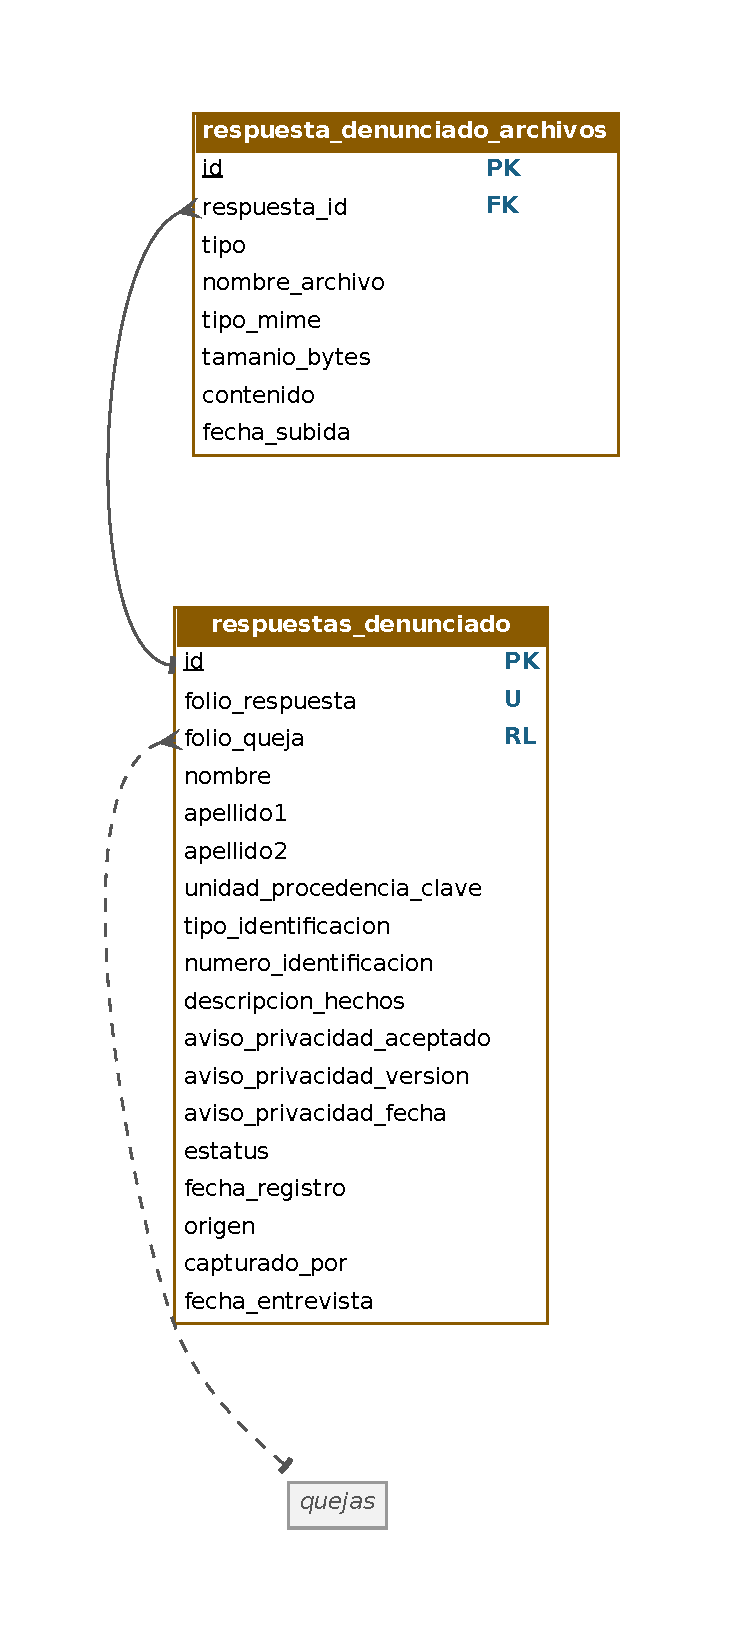
\includegraphics[width=\textwidth,height=0.85\textheight,keepaspectratio]{images/er_grupo_07.pdf}
	\caption{Diagrama entidad-relación: \texttt{respuestas\_denunciado}, \texttt{respuesta\_denunciado\_archivos}}
	\label{fig:er_grupo_07}
\end{figure}

\subsection{Tabla \texttt{respuesta\_denunciado\_archivos}}
Archivos de evidencia que acompañan la respuesta de la persona señalada. Servicio responsable: denunciado-service.


\rowcolors{2}{rowblue}{white}
\footnotesize
\renewcommand{\arraystretch}{1.15}
\setlength{\tabcolsep}{4pt}
\begin{longtable}{|L{3.9cm}|L{2.4cm}|L{0.9cm}|L{1.2cm}|L{6.6cm}|}
	\hiderowcolors\caption{Diccionario de datos de la tabla \texttt{respuesta\_denunciado\_archivos}}
	\label{tab:dic_respuesta_denunciado_archivos} \\ \showrowcolors
	\hline
	\rowcolor{headerblue}
	\headercell{Columna} & \headercell{Tipo} & \headercell{Nulo} & \headercell{Clave} & \headercell{Descripción} \\
	\hline
	\endfirsthead
	\hline
	\rowcolor{headerblue}
	\headercell{Columna} & \headercell{Tipo} & \headercell{Nulo} & \headercell{Clave} & \headercell{Descripción} \\
	\hline
	\endhead
		\texttt{id} & BIGINT & No & PK & Identificador único del registro, generado automáticamente. \\ \hline
		\texttt{respuesta\_\allowbreak{}id} & BIGINT & No & FK & Respuesta a la que pertenece el archivo. \\ \hline
		\texttt{tipo} & VARCHAR(20) & No &  & Clasificación del archivo. \\ \hline
		\texttt{nombre\_\allowbreak{}archivo} & VARCHAR(255) & No &  & Nombre original del archivo. \\ \hline
		\texttt{tipo\_\allowbreak{}mime} & VARCHAR(100) & No &  & Tipo MIME del archivo. \\ \hline
		\texttt{tamanio\_\allowbreak{}bytes} & BIGINT & No &  & Tamaño del archivo en bytes. \\ \hline
		\texttt{contenido} & BYTEA & No &  & Contenido binario del archivo. \\ \hline
		\texttt{fecha\_\allowbreak{}subida} & TIMESTAMP & No &  & Fecha y hora en que se subió el archivo. \\ \hline
\end{longtable}
\normalsize
\setlength{\tabcolsep}{6pt}
\renewcommand{\arraystretch}{1}

\subsection{Tabla \texttt{respuestas\_denunciado}}
Versión de los hechos rendida por la persona señalada, ya sea capturada por ella misma o registrada por el analista. Servicio responsable: denunciado-service.


\rowcolors{2}{rowblue}{white}
\footnotesize
\renewcommand{\arraystretch}{1.15}
\setlength{\tabcolsep}{4pt}
\begin{longtable}{|L{3.9cm}|L{2.4cm}|L{0.9cm}|L{1.2cm}|L{6.6cm}|}
	\hiderowcolors\caption{Diccionario de datos de la tabla \texttt{respuestas\_denunciado}}
	\label{tab:dic_respuestas_denunciado} \\ \showrowcolors
	\hline
	\rowcolor{headerblue}
	\headercell{Columna} & \headercell{Tipo} & \headercell{Nulo} & \headercell{Clave} & \headercell{Descripción} \\
	\hline
	\endfirsthead
	\hline
	\rowcolor{headerblue}
	\headercell{Columna} & \headercell{Tipo} & \headercell{Nulo} & \headercell{Clave} & \headercell{Descripción} \\
	\hline
	\endhead
		\texttt{id} & BIGINT & No & PK & Identificador único del registro, generado automáticamente. \\ \hline
		\texttt{folio\_\allowbreak{}respuesta} & VARCHAR(20) & No & U & Folio único de la respuesta. \\ \hline
		\texttt{folio\_\allowbreak{}queja} & VARCHAR(20) & No & RL & Folio de la queja original. \\ \hline
		\texttt{nombre} & VARCHAR(50) & No &  & Nombre de la persona señalada. \\ \hline
		\texttt{apellido1} & VARCHAR(50) & No &  & Primer apellido de la persona señalada. \\ \hline
		\texttt{apellido2} & VARCHAR(50) & Sí &  & Segundo apellido de la persona señalada. \\ \hline
		\texttt{unidad\_\allowbreak{}procedencia\_\allowbreak{}clave} & VARCHAR(40) & No &  & Clave de la unidad de procedencia de la persona señalada. \\ \hline
		\texttt{tipo\_\allowbreak{}identificacion} & VARCHAR(20) & No &  & Tipo de identificación (boleta o número de empleado). \\ \hline
		\texttt{numero\_\allowbreak{}identificacion} & VARCHAR(10) & No &  & Número de identificación (boleta o número de empleado). \\ \hline
		\texttt{descripcion\_\allowbreak{}hechos} & TEXT & No &  & Versión de los hechos de la persona señalada. \\ \hline
		\texttt{aviso\_\allowbreak{}privacidad\_\allowbreak{}aceptado} & BOOLEAN & No &  & Indica si se aceptó el aviso de privacidad. \\ \hline
		\texttt{aviso\_\allowbreak{}privacidad\_\allowbreak{}version} & VARCHAR(10) & Sí &  & Versión del aviso de privacidad aceptada. \\ \hline
		\texttt{aviso\_\allowbreak{}privacidad\_\allowbreak{}fecha} & TIMESTAMP & Sí &  & Fecha y hora de aceptación del aviso de privacidad. \\ \hline
		\texttt{estatus} & VARCHAR(20) & No &  & Estado de la respuesta. \\ \hline
		\texttt{fecha\_\allowbreak{}registro} & TIMESTAMP & No &  & Fecha y hora del registro. \\ \hline
		\texttt{origen} & VARCHAR(20) & Sí &  & Quién capturó la respuesta (la persona señalada o el analista). \\ \hline
		\texttt{capturado\_\allowbreak{}por} & VARCHAR(120) & Sí &  & Analista que capturó la respuesta, si aplica. \\ \hline
		\texttt{fecha\_\allowbreak{}entrevista} & DATE & Sí &  & Fecha de la entrevista con la persona señalada. \\ \hline
\end{longtable}
\normalsize
\setlength{\tabcolsep}{6pt}
\renewcommand{\arraystretch}{1}

\section{Módulo: Subdefensoría}
\label{anx:bd_mod4}

Las figuras de esta sección muestran el diagrama entidad-relación del módulo con todas sus columnas, divididas en grupos de tablas para facilitar su lectura. Las tablas en gris pertenecen a otros grupos o módulos y se incluyen solo para mostrar las relaciones.


\begin{figure}[H]
	\centering
	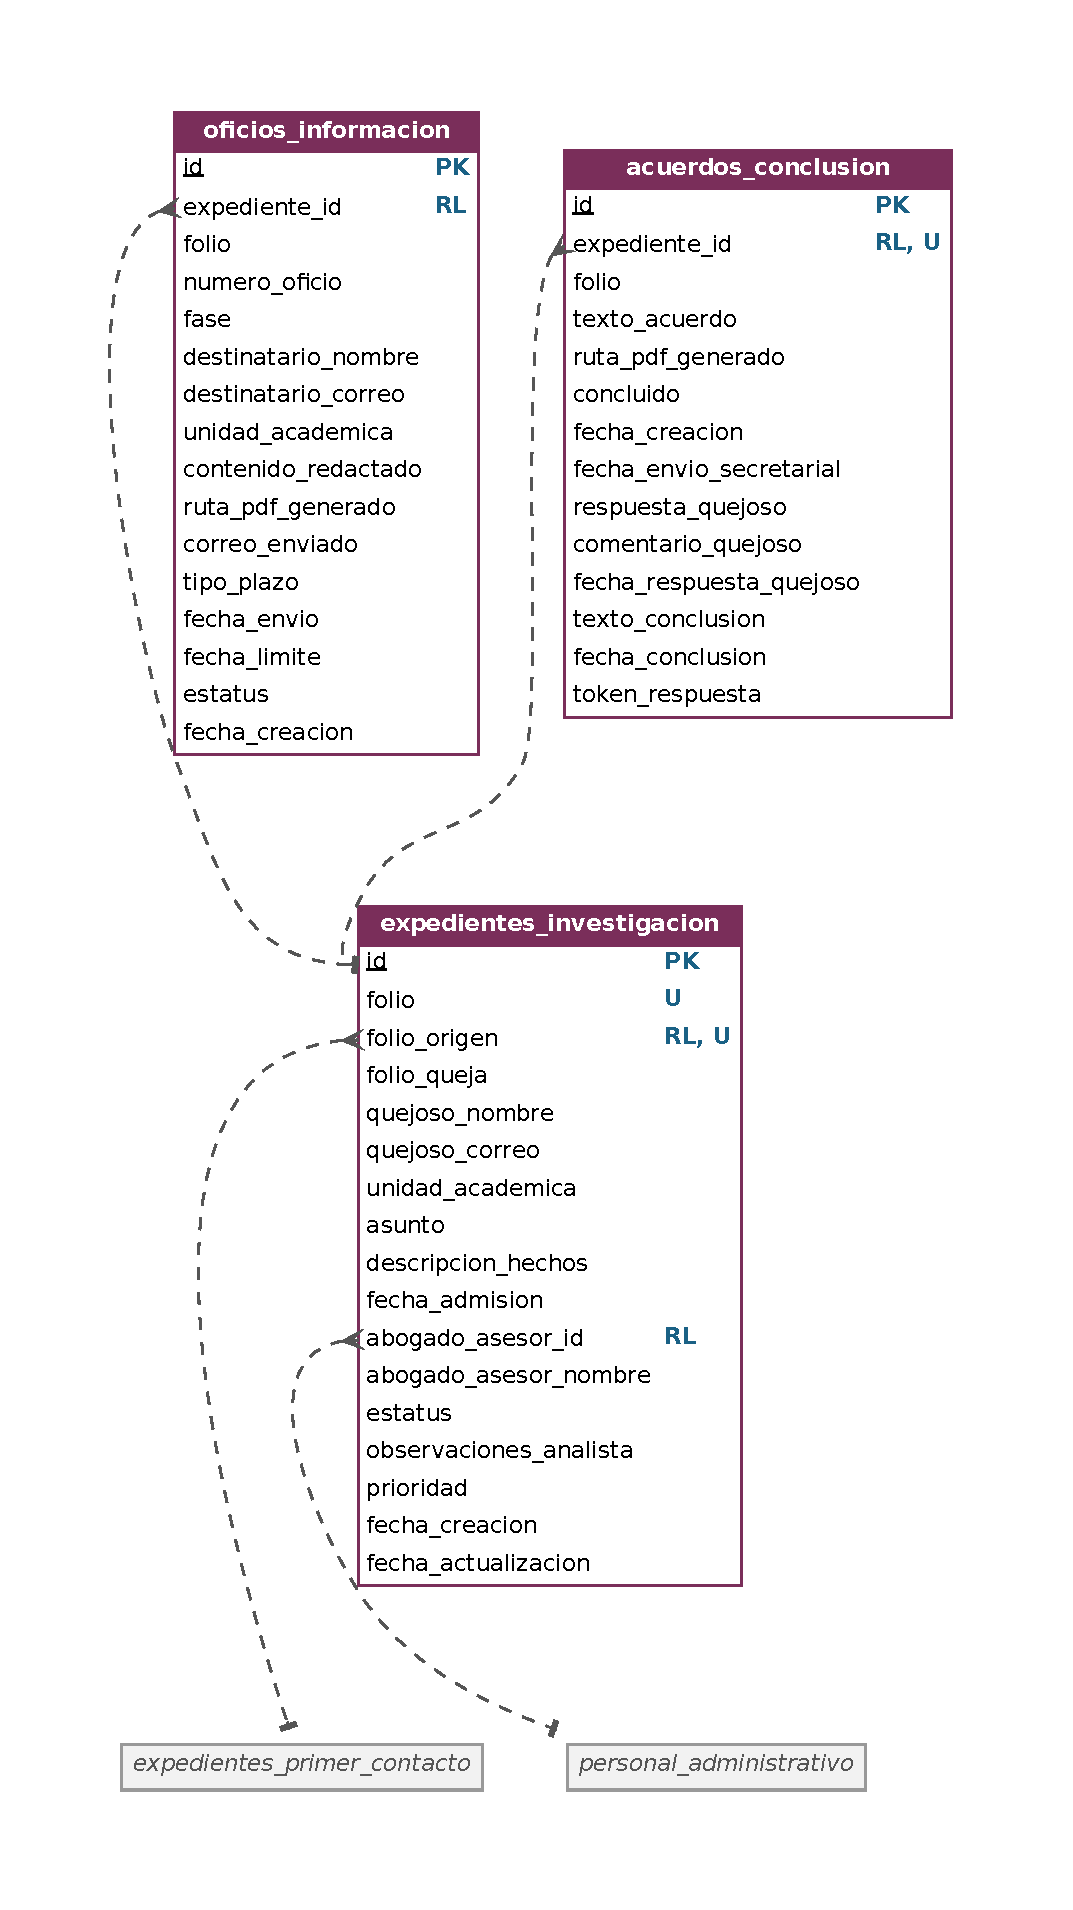
\includegraphics[width=\textwidth,height=0.85\textheight,keepaspectratio]{images/er_grupo_08.pdf}
	\caption{Diagrama entidad-relación: \texttt{expedientes\_investigacion}, \texttt{oficios\_informacion}, \texttt{acuerdos\_conclusion}}
	\label{fig:er_grupo_08}
\end{figure}


\begin{figure}[H]
	\centering
	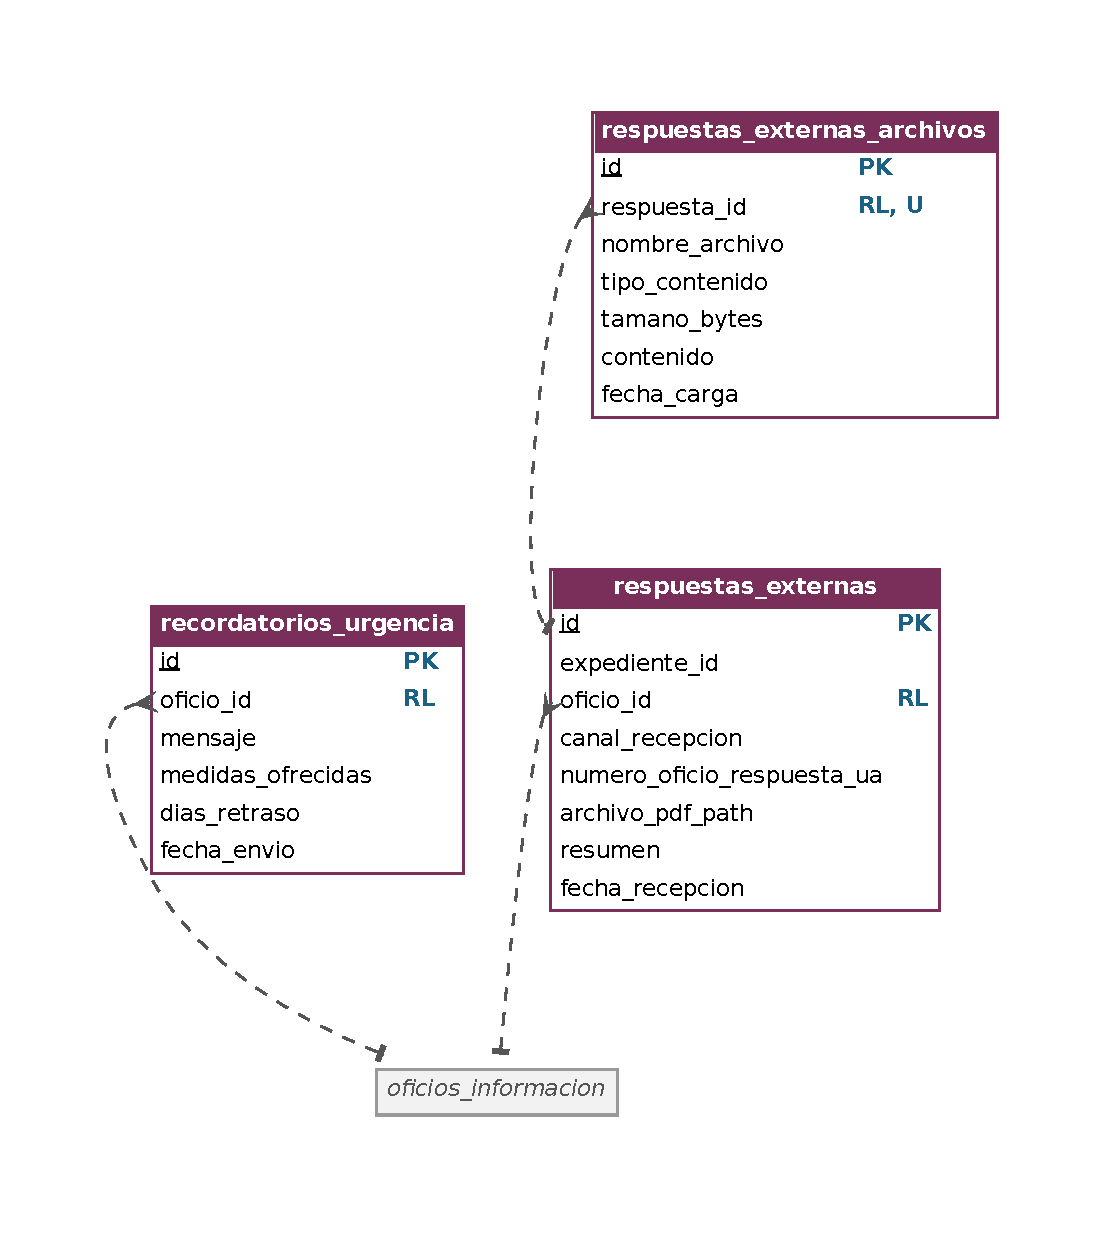
\includegraphics[width=\textwidth,height=0.85\textheight,keepaspectratio]{images/er_grupo_09.pdf}
	\caption{Diagrama entidad-relación: \texttt{recordatorios\_urgencia}, \texttt{respuestas\_externas}, \texttt{respuestas\_externas\_archivos}}
	\label{fig:er_grupo_09}
\end{figure}

\subsection{Tabla \texttt{acuerdos\_conclusion}}
Acuerdo de conciliación y de conclusión con el que se cierra un expediente de investigación, junto con la respuesta del quejoso. Servicio responsable: subdefensoria-service.


\rowcolors{2}{rowblue}{white}
\footnotesize
\renewcommand{\arraystretch}{1.15}
\setlength{\tabcolsep}{4pt}
\begin{longtable}{|L{3.9cm}|L{2.4cm}|L{0.9cm}|L{1.2cm}|L{6.6cm}|}
	\hiderowcolors\caption{Diccionario de datos de la tabla \texttt{acuerdos\_conclusion}}
	\label{tab:dic_acuerdos_conclusion} \\ \showrowcolors
	\hline
	\rowcolor{headerblue}
	\headercell{Columna} & \headercell{Tipo} & \headercell{Nulo} & \headercell{Clave} & \headercell{Descripción} \\
	\hline
	\endfirsthead
	\hline
	\rowcolor{headerblue}
	\headercell{Columna} & \headercell{Tipo} & \headercell{Nulo} & \headercell{Clave} & \headercell{Descripción} \\
	\hline
	\endhead
		\texttt{id} & BIGINT & No & PK & Identificador único del registro, generado automáticamente. \\ \hline
		\texttt{expediente\_\allowbreak{}id} & BIGINT & No & RL, U & Expediente al que pertenece el registro. \\ \hline
		\texttt{folio} & VARCHAR(50) & No &  & Folio del expediente de investigación. \\ \hline
		\texttt{texto\_\allowbreak{}acuerdo} & TEXT & No &  & Texto del acuerdo de conciliación. \\ \hline
		\texttt{ruta\_\allowbreak{}pdf\_\allowbreak{}generado} & VARCHAR(300) & Sí &  & Ruta del PDF generado. \\ \hline
		\texttt{concluido} & BOOLEAN & No &  & Indica si el expediente quedó concluido. \\ \hline
		\texttt{fecha\_\allowbreak{}creacion} & TIMESTAMP & No &  & Fecha y hora de creación del registro. \\ \hline
		\texttt{fecha\_\allowbreak{}envio\_\allowbreak{}secretarial} & TIMESTAMP & Sí &  & Fecha de envío del acuerdo para firma. \\ \hline
		\texttt{respuesta\_\allowbreak{}quejoso} & VARCHAR(20) & Sí &  & Respuesta del quejoso al acuerdo (acepta o rechaza). \\ \hline
		\texttt{comentario\_\allowbreak{}quejoso} & TEXT & Sí &  & Comentario del quejoso al responder. \\ \hline
		\texttt{fecha\_\allowbreak{}respuesta\_\allowbreak{}quejoso} & TIMESTAMP & Sí &  & Fecha y hora de la respuesta del quejoso. \\ \hline
		\texttt{texto\_\allowbreak{}conclusion} & TEXT & Sí &  & Texto del acuerdo de conclusión. \\ \hline
		\texttt{fecha\_\allowbreak{}conclusion} & TIMESTAMP & Sí &  & Fecha de conclusión del expediente. \\ \hline
		\texttt{token\_\allowbreak{}respuesta} & VARCHAR(64) & Sí &  & Token del enlace con el que la persona responde sin iniciar sesión. \\ \hline
\end{longtable}
\normalsize
\setlength{\tabcolsep}{6pt}
\renewcommand{\arraystretch}{1}

\subsection{Tabla \texttt{expedientes\_investigacion}}
Expediente de investigación que se crea cuando Primer Contacto dictamina una queja como procedente; registra el abogado asignado, la etapa y la prioridad. Servicio responsable: subdefensoria-service.


\rowcolors{2}{rowblue}{white}
\footnotesize
\renewcommand{\arraystretch}{1.15}
\setlength{\tabcolsep}{4pt}
\begin{longtable}{|L{3.9cm}|L{2.4cm}|L{0.9cm}|L{1.2cm}|L{6.6cm}|}
	\hiderowcolors\caption{Diccionario de datos de la tabla \texttt{expedientes\_investigacion}}
	\label{tab:dic_expedientes_investigacion} \\ \showrowcolors
	\hline
	\rowcolor{headerblue}
	\headercell{Columna} & \headercell{Tipo} & \headercell{Nulo} & \headercell{Clave} & \headercell{Descripción} \\
	\hline
	\endfirsthead
	\hline
	\rowcolor{headerblue}
	\headercell{Columna} & \headercell{Tipo} & \headercell{Nulo} & \headercell{Clave} & \headercell{Descripción} \\
	\hline
	\endhead
		\texttt{id} & BIGINT & No & PK & Identificador único del registro, generado automáticamente. \\ \hline
		\texttt{folio} & VARCHAR(50) & No & U & Folio del expediente en Subdefensoría. \\ \hline
		\texttt{folio\_\allowbreak{}origen} & VARCHAR(50) & No & RL, U & Folio del expediente en Primer Contacto. \\ \hline
		\texttt{folio\_\allowbreak{}queja} & VARCHAR(50) & Sí &  & Folio de la queja original. \\ \hline
		\texttt{quejoso\_\allowbreak{}nombre} & VARCHAR(150) & Sí &  & Nombre del quejoso. \\ \hline
		\texttt{quejoso\_\allowbreak{}correo} & VARCHAR(150) & Sí &  & Correo electrónico del quejoso. \\ \hline
		\texttt{unidad\_\allowbreak{}academica} & VARCHAR(100) & Sí &  & Unidad académica relacionada. \\ \hline
		\texttt{asunto} & VARCHAR(200) & Sí &  & Asunto o tema del documento. \\ \hline
		\texttt{descripcion\_\allowbreak{}hechos} & TEXT & Sí &  & Narrativa de los hechos de la queja. \\ \hline
		\texttt{fecha\_\allowbreak{}admision} & DATE & No &  & Fecha en que el expediente se admitió en Subdefensoría. \\ \hline
		\texttt{abogado\_\allowbreak{}asesor\_\allowbreak{}id} & BIGINT & Sí & RL & Identificador del abogado de Subdefensoría asignado (personal administrativo). \\ \hline
		\texttt{abogado\_\allowbreak{}asesor\_\allowbreak{}nombre} & VARCHAR(150) & Sí &  & Nombre del abogado asignado, conservado para consulta. \\ \hline
		\texttt{estatus} & VARCHAR(30) & No &  & Etapa de la investigación (RECIBIDO, EN\_INVESTIGACION, EN\_ESPERA\_OFICIO, CONCLUIDO, entre otras). \\ \hline
		\texttt{observaciones\_\allowbreak{}analista} & TEXT & Sí &  & Observaciones del analista de Primer Contacto al turnar. \\ \hline
		\texttt{prioridad} & VARCHAR(10) & Sí &  & Prioridad del expediente (baja, media, alta o urgente). \\ \hline
		\texttt{fecha\_\allowbreak{}creacion} & TIMESTAMP & No &  & Fecha y hora de creación del registro. \\ \hline
		\texttt{fecha\_\allowbreak{}actualizacion} & TIMESTAMP & Sí &  & Fecha y hora de la última actualización. \\ \hline
\end{longtable}
\normalsize
\setlength{\tabcolsep}{6pt}
\renewcommand{\arraystretch}{1}

\subsection{Tabla \texttt{oficios\_informacion}}
Oficios de solicitud de información enviados a las unidades, con su plazo y fecha límite. Servicio responsable: subdefensoria-service.


\rowcolors{2}{rowblue}{white}
\footnotesize
\renewcommand{\arraystretch}{1.15}
\setlength{\tabcolsep}{4pt}
\begin{longtable}{|L{3.9cm}|L{2.4cm}|L{0.9cm}|L{1.2cm}|L{6.6cm}|}
	\hiderowcolors\caption{Diccionario de datos de la tabla \texttt{oficios\_informacion}}
	\label{tab:dic_oficios_informacion} \\ \showrowcolors
	\hline
	\rowcolor{headerblue}
	\headercell{Columna} & \headercell{Tipo} & \headercell{Nulo} & \headercell{Clave} & \headercell{Descripción} \\
	\hline
	\endfirsthead
	\hline
	\rowcolor{headerblue}
	\headercell{Columna} & \headercell{Tipo} & \headercell{Nulo} & \headercell{Clave} & \headercell{Descripción} \\
	\hline
	\endhead
		\texttt{id} & BIGINT & No & PK & Identificador único del registro, generado automáticamente. \\ \hline
		\texttt{expediente\_\allowbreak{}id} & BIGINT & No & RL & Expediente al que pertenece el registro. \\ \hline
		\texttt{folio} & VARCHAR(50) & No &  & Folio del expediente de investigación. \\ \hline
		\texttt{numero\_\allowbreak{}oficio} & VARCHAR(50) & No &  & Número del oficio. \\ \hline
		\texttt{fase} & VARCHAR(30) & No &  & Fase del oficio (primera solicitud o recordatorio). \\ \hline
		\texttt{destinatario\_\allowbreak{}nombre} & VARCHAR(200) & No &  & Nombre del titular de la unidad destinataria. \\ \hline
		\texttt{destinatario\_\allowbreak{}correo} & VARCHAR(150) & No &  & Correo electrónico del titular de la unidad destinataria. \\ \hline
		\texttt{unidad\_\allowbreak{}academica} & VARCHAR(100) & Sí &  & Unidad académica relacionada. \\ \hline
		\texttt{contenido\_\allowbreak{}redactado} & TEXT & No &  & Texto del oficio redactado. \\ \hline
		\texttt{ruta\_\allowbreak{}pdf\_\allowbreak{}generado} & VARCHAR(300) & Sí &  & Ruta del PDF generado. \\ \hline
		\texttt{correo\_\allowbreak{}enviado} & BOOLEAN & Sí &  & Indica si el correo se envió correctamente. \\ \hline
		\texttt{tipo\_\allowbreak{}plazo} & VARCHAR(20) & No &  & Plazo aplicable al oficio (diez o cinco días hábiles). \\ \hline
		\texttt{fecha\_\allowbreak{}envio} & DATE & No &  & Fecha de envío. \\ \hline
		\texttt{fecha\_\allowbreak{}limite} & DATE & No &  & Fecha límite de respuesta según el plazo aplicable. \\ \hline
		\texttt{estatus} & VARCHAR(20) & No &  & Estado del oficio. \\ \hline
		\texttt{fecha\_\allowbreak{}creacion} & TIMESTAMP & No &  & Fecha y hora de creación del registro. \\ \hline
\end{longtable}
\normalsize
\setlength{\tabcolsep}{6pt}
\renewcommand{\arraystretch}{1}

\subsection{Tabla \texttt{recordatorios\_urgencia}}
Recordatorios enviados cuando una unidad no responde un oficio dentro del plazo. Servicio responsable: subdefensoria-service.


\rowcolors{2}{rowblue}{white}
\footnotesize
\renewcommand{\arraystretch}{1.15}
\setlength{\tabcolsep}{4pt}
\begin{longtable}{|L{3.9cm}|L{2.4cm}|L{0.9cm}|L{1.2cm}|L{6.6cm}|}
	\hiderowcolors\caption{Diccionario de datos de la tabla \texttt{recordatorios\_urgencia}}
	\label{tab:dic_recordatorios_urgencia} \\ \showrowcolors
	\hline
	\rowcolor{headerblue}
	\headercell{Columna} & \headercell{Tipo} & \headercell{Nulo} & \headercell{Clave} & \headercell{Descripción} \\
	\hline
	\endfirsthead
	\hline
	\rowcolor{headerblue}
	\headercell{Columna} & \headercell{Tipo} & \headercell{Nulo} & \headercell{Clave} & \headercell{Descripción} \\
	\hline
	\endhead
		\texttt{id} & BIGINT & No & PK & Identificador único del registro, generado automáticamente. \\ \hline
		\texttt{oficio\_\allowbreak{}id} & BIGINT & No & RL & Oficio al que corresponde el registro. \\ \hline
		\texttt{mensaje} & TEXT & No &  & Texto del mensaje. \\ \hline
		\texttt{medidas\_\allowbreak{}ofrecidas} & TEXT & Sí &  & Medidas ofrecidas a la unidad en el recordatorio. \\ \hline
		\texttt{dias\_\allowbreak{}retraso} & INTEGER & No &  & Días transcurridos desde el vencimiento del plazo. \\ \hline
		\texttt{fecha\_\allowbreak{}envio} & TIMESTAMP & No &  & Fecha de envío. \\ \hline
\end{longtable}
\normalsize
\setlength{\tabcolsep}{6pt}
\renewcommand{\arraystretch}{1}

\subsection{Tabla \texttt{respuestas\_externas}}
Respuestas recibidas de las unidades a los oficios de solicitud de información. Servicio responsable: subdefensoria-service.


\rowcolors{2}{rowblue}{white}
\footnotesize
\renewcommand{\arraystretch}{1.15}
\setlength{\tabcolsep}{4pt}
\begin{longtable}{|L{3.9cm}|L{2.4cm}|L{0.9cm}|L{1.2cm}|L{6.6cm}|}
	\hiderowcolors\caption{Diccionario de datos de la tabla \texttt{respuestas\_externas}}
	\label{tab:dic_respuestas_externas} \\ \showrowcolors
	\hline
	\rowcolor{headerblue}
	\headercell{Columna} & \headercell{Tipo} & \headercell{Nulo} & \headercell{Clave} & \headercell{Descripción} \\
	\hline
	\endfirsthead
	\hline
	\rowcolor{headerblue}
	\headercell{Columna} & \headercell{Tipo} & \headercell{Nulo} & \headercell{Clave} & \headercell{Descripción} \\
	\hline
	\endhead
		\texttt{id} & BIGINT & No & PK & Identificador único del registro, generado automáticamente. \\ \hline
		\texttt{expediente\_\allowbreak{}id} & BIGINT & No &  & Expediente al que pertenece el registro. \\ \hline
		\texttt{oficio\_\allowbreak{}id} & BIGINT & No & RL & Oficio al que corresponde el registro. \\ \hline
		\texttt{canal\_\allowbreak{}recepcion} & VARCHAR(100) & No &  & Medio por el que se recibió la respuesta (correo, oficio físico, etc.). \\ \hline
		\texttt{numero\_\allowbreak{}oficio\_\allowbreak{}respuesta\_\allowbreak{}ua} & VARCHAR(100) & Sí &  & Número del oficio con el que respondió la unidad. \\ \hline
		\texttt{archivo\_\allowbreak{}pdf\_\allowbreak{}path} & VARCHAR(300) & Sí &  & Ruta del archivo PDF de la respuesta. \\ \hline
		\texttt{resumen} & TEXT & No &  & Texto del resumen. \\ \hline
		\texttt{fecha\_\allowbreak{}recepcion} & TIMESTAMP & No &  & Fecha y hora de recepción. \\ \hline
\end{longtable}
\normalsize
\setlength{\tabcolsep}{6pt}
\renewcommand{\arraystretch}{1}

\subsection{Tabla \texttt{respuestas\_externas\_archivos}}
Archivo digital asociado a la respuesta de una unidad. Servicio responsable: subdefensoria-service.


\rowcolors{2}{rowblue}{white}
\footnotesize
\renewcommand{\arraystretch}{1.15}
\setlength{\tabcolsep}{4pt}
\begin{longtable}{|L{3.9cm}|L{2.4cm}|L{0.9cm}|L{1.2cm}|L{6.6cm}|}
	\hiderowcolors\caption{Diccionario de datos de la tabla \texttt{respuestas\_externas\_archivos}}
	\label{tab:dic_respuestas_externas_archivos} \\ \showrowcolors
	\hline
	\rowcolor{headerblue}
	\headercell{Columna} & \headercell{Tipo} & \headercell{Nulo} & \headercell{Clave} & \headercell{Descripción} \\
	\hline
	\endfirsthead
	\hline
	\rowcolor{headerblue}
	\headercell{Columna} & \headercell{Tipo} & \headercell{Nulo} & \headercell{Clave} & \headercell{Descripción} \\
	\hline
	\endhead
		\texttt{id} & BIGINT & No & PK & Identificador único del registro, generado automáticamente. \\ \hline
		\texttt{respuesta\_\allowbreak{}id} & BIGINT & No & RL, U & Respuesta a la que pertenece el archivo. \\ \hline
		\texttt{nombre\_\allowbreak{}archivo} & VARCHAR(255) & No &  & Nombre original del archivo. \\ \hline
		\texttt{tipo\_\allowbreak{}contenido} & VARCHAR(50) & No &  & Tipo MIME del archivo. \\ \hline
		\texttt{tamano\_\allowbreak{}bytes} & BIGINT & No &  & Tamaño del archivo en bytes. \\ \hline
		\texttt{contenido} & BYTEA & No &  & Contenido binario del archivo. \\ \hline
		\texttt{fecha\_\allowbreak{}carga} & TIMESTAMP & No &  & Fecha de carga del archivo. \\ \hline
\end{longtable}
\normalsize
\setlength{\tabcolsep}{6pt}
\renewcommand{\arraystretch}{1}

\section{Módulo: Administración y catálogos}
\label{anx:bd_mod5}

Las figuras de esta sección muestran el diagrama entidad-relación del módulo con todas sus columnas, divididas en grupos de tablas para facilitar su lectura. Las tablas en gris pertenecen a otros grupos o módulos y se incluyen solo para mostrar las relaciones.


\begin{figure}[H]
	\centering
	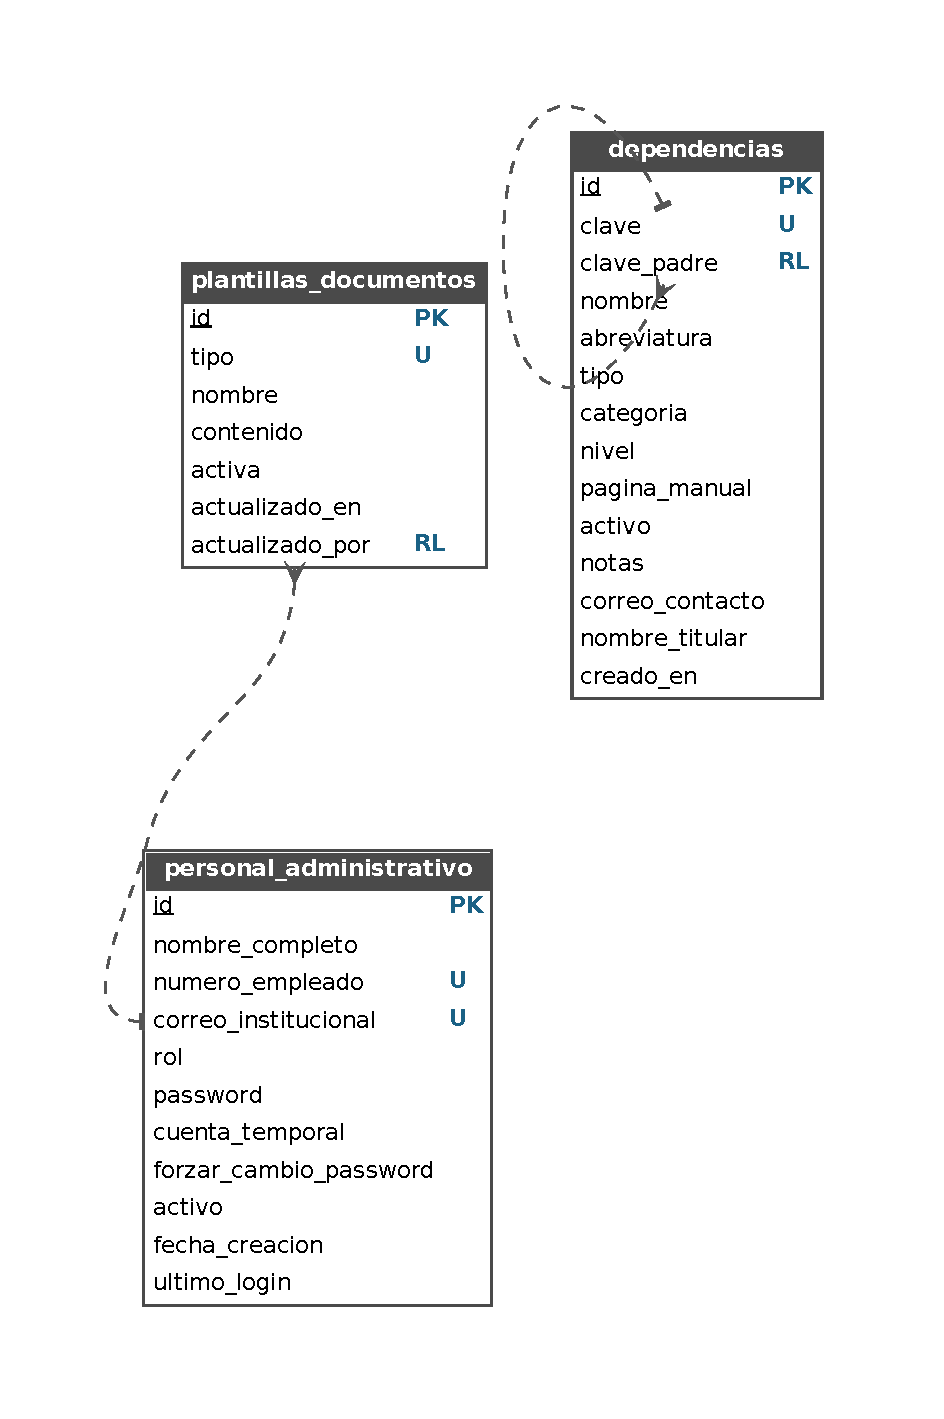
\includegraphics[width=\textwidth,height=0.85\textheight,keepaspectratio]{images/er_grupo_10.pdf}
	\caption{Diagrama entidad-relación: \texttt{personal\_administrativo}, \texttt{dependencias}, \texttt{plantillas\_documentos}}
	\label{fig:er_grupo_10}
\end{figure}


\begin{figure}[H]
	\centering
	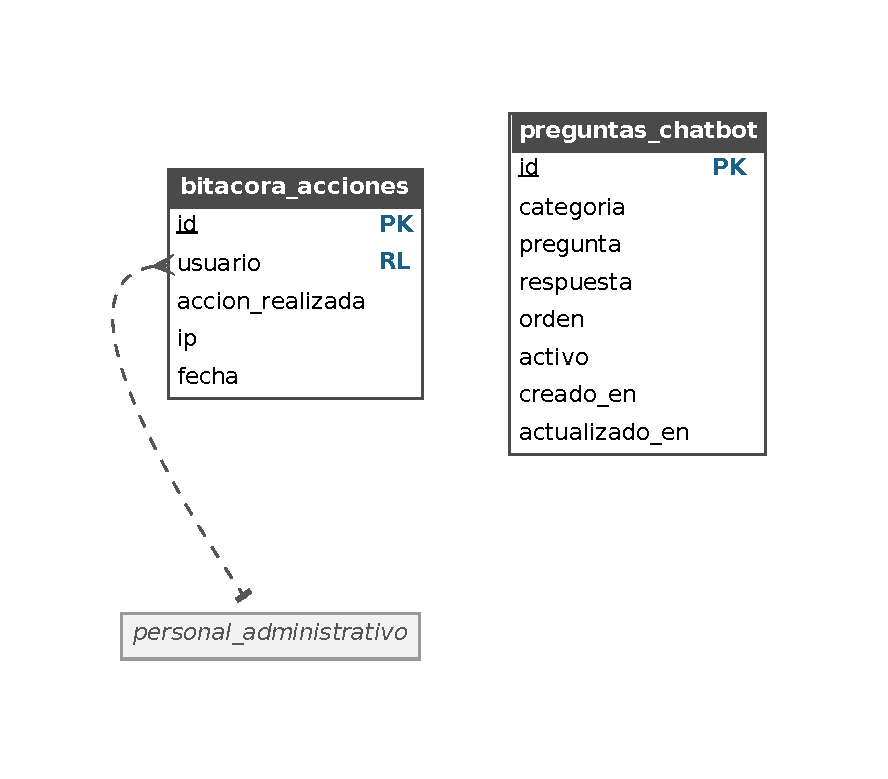
\includegraphics[width=\textwidth,height=0.85\textheight,keepaspectratio]{images/er_grupo_11.pdf}
	\caption{Diagrama entidad-relación: \texttt{bitacora\_acciones}, \texttt{preguntas\_chatbot}}
	\label{fig:er_grupo_11}
\end{figure}

\subsection{Tabla \texttt{bitacora\_acciones}}
Bitácora de auditoría de las acciones administrativas: usuario, acción, dirección de origen y fecha. Servicio responsable: admin-service.


\rowcolors{2}{rowblue}{white}
\footnotesize
\renewcommand{\arraystretch}{1.15}
\setlength{\tabcolsep}{4pt}
\begin{longtable}{|L{3.9cm}|L{2.4cm}|L{0.9cm}|L{1.2cm}|L{6.6cm}|}
	\hiderowcolors\caption{Diccionario de datos de la tabla \texttt{bitacora\_acciones}}
	\label{tab:dic_bitacora_acciones} \\ \showrowcolors
	\hline
	\rowcolor{headerblue}
	\headercell{Columna} & \headercell{Tipo} & \headercell{Nulo} & \headercell{Clave} & \headercell{Descripción} \\
	\hline
	\endfirsthead
	\hline
	\rowcolor{headerblue}
	\headercell{Columna} & \headercell{Tipo} & \headercell{Nulo} & \headercell{Clave} & \headercell{Descripción} \\
	\hline
	\endhead
		\texttt{id} & BIGINT & No & PK & Identificador único del registro, generado automáticamente. \\ \hline
		\texttt{usuario} & VARCHAR(255) & No & RL & Usuario que realizó la acción. \\ \hline
		\texttt{accion\_\allowbreak{}realizada} & VARCHAR(255) & No &  & Descripción de la acción administrativa realizada. \\ \hline
		\texttt{ip} & VARCHAR(255) & No &  & Dirección IP de origen de la acción. \\ \hline
		\texttt{fecha} & TIMESTAMP & No &  & Fecha y hora de la acción. \\ \hline
\end{longtable}
\normalsize
\setlength{\tabcolsep}{6pt}
\renewcommand{\arraystretch}{1}

\subsection{Tabla \texttt{dependencias}}
Catálogo jerárquico de dependencias y unidades académicas del Instituto, con su titular y correo de contacto. Servicio responsable: catalogo-service.


\rowcolors{2}{rowblue}{white}
\footnotesize
\renewcommand{\arraystretch}{1.15}
\setlength{\tabcolsep}{4pt}
\begin{longtable}{|L{3.9cm}|L{2.4cm}|L{0.9cm}|L{1.2cm}|L{6.6cm}|}
	\hiderowcolors\caption{Diccionario de datos de la tabla \texttt{dependencias}}
	\label{tab:dic_dependencias} \\ \showrowcolors
	\hline
	\rowcolor{headerblue}
	\headercell{Columna} & \headercell{Tipo} & \headercell{Nulo} & \headercell{Clave} & \headercell{Descripción} \\
	\hline
	\endfirsthead
	\hline
	\rowcolor{headerblue}
	\headercell{Columna} & \headercell{Tipo} & \headercell{Nulo} & \headercell{Clave} & \headercell{Descripción} \\
	\hline
	\endhead
		\texttt{id} & BIGINT & No & PK & Identificador único del registro, generado automáticamente. \\ \hline
		\texttt{clave} & VARCHAR(20) & No & U & Clave única de la dependencia. \\ \hline
		\texttt{clave\_\allowbreak{}padre} & VARCHAR(20) & Sí & RL & Clave de la dependencia superior en la jerarquía. \\ \hline
		\texttt{nombre} & VARCHAR(255) & No &  & Nombre oficial de la dependencia. \\ \hline
		\texttt{abreviatura} & VARCHAR(30) & Sí &  & Abreviatura o siglas de la dependencia. \\ \hline
		\texttt{tipo} & VARCHAR(60) & No &  & Tipo de dependencia. \\ \hline
		\texttt{categoria} & VARCHAR(150) & Sí &  & Categoría de la dependencia (escuela superior, centro de investigación, etc.). \\ \hline
		\texttt{nivel} & INTEGER & No &  & Nivel jerárquico de la dependencia. \\ \hline
		\texttt{pagina\_\allowbreak{}manual} & INTEGER & Sí &  & Página del manual de organización donde aparece la dependencia. \\ \hline
		\texttt{activo} & BOOLEAN & No &  & Indica si el registro está activo. \\ \hline
		\texttt{notas} & TEXT & Sí &  & Notas adicionales. \\ \hline
		\texttt{correo\_\allowbreak{}contacto} & VARCHAR(150) & Sí &  & Correo electrónico de contacto de la dependencia. \\ \hline
		\texttt{nombre\_\allowbreak{}titular} & VARCHAR(150) & Sí &  & Nombre del titular de la dependencia. \\ \hline
		\texttt{creado\_\allowbreak{}en} & TIMESTAMP & Sí &  & Fecha y hora de creación. \\ \hline
\end{longtable}
\normalsize
\setlength{\tabcolsep}{6pt}
\renewcommand{\arraystretch}{1}

\subsection{Tabla \texttt{personal\_administrativo}}
Cuentas del personal de la Defensoría con su rol, estado de la cuenta y último acceso. Servicio responsable: admin-service, revision-service, primer-contacto-service.


\rowcolors{2}{rowblue}{white}
\footnotesize
\renewcommand{\arraystretch}{1.15}
\setlength{\tabcolsep}{4pt}
\begin{longtable}{|L{3.9cm}|L{2.4cm}|L{0.9cm}|L{1.2cm}|L{6.6cm}|}
	\hiderowcolors\caption{Diccionario de datos de la tabla \texttt{personal\_administrativo}}
	\label{tab:dic_personal_administrativo} \\ \showrowcolors
	\hline
	\rowcolor{headerblue}
	\headercell{Columna} & \headercell{Tipo} & \headercell{Nulo} & \headercell{Clave} & \headercell{Descripción} \\
	\hline
	\endfirsthead
	\hline
	\rowcolor{headerblue}
	\headercell{Columna} & \headercell{Tipo} & \headercell{Nulo} & \headercell{Clave} & \headercell{Descripción} \\
	\hline
	\endhead
		\texttt{id} & BIGINT & No & PK & Identificador único del registro, generado automáticamente. \\ \hline
		\texttt{nombre\_\allowbreak{}completo} & VARCHAR(255) & No &  & Nombre completo de la persona. \\ \hline
		\texttt{numero\_\allowbreak{}empleado} & VARCHAR(255) & No & U & Número de empleado. \\ \hline
		\texttt{correo\_\allowbreak{}institucional} & VARCHAR(255) & No & U & Correo institucional; se usa para iniciar sesión. \\ \hline
		\texttt{rol} & VARCHAR(255) & No &  & Rol del usuario (RECEPCIONISTA, ANALISTA\_PRIMER\_CONTACTO, SUBDEFENSOR o DEFENSOR). \\ \hline
		\texttt{password} & VARCHAR(255) & No &  & Contraseña cifrada mediante función de resumen. \\ \hline
		\texttt{cuenta\_\allowbreak{}temporal} & BOOLEAN & No &  & Indica si la cuenta conserva la contraseña temporal. \\ \hline
		\texttt{forzar\_\allowbreak{}cambio\_\allowbreak{}password} & BOOLEAN & No &  & Indica si el usuario debe cambiar su contraseña en el siguiente inicio de sesión. \\ \hline
		\texttt{activo} & BOOLEAN & No &  & Indica si la cuenta está activa; dar de baja la desactiva sin eliminarla. \\ \hline
		\texttt{fecha\_\allowbreak{}creacion} & TIMESTAMP & No &  & Fecha y hora de creación del registro. \\ \hline
		\texttt{ultimo\_\allowbreak{}login} & TIMESTAMP & Sí &  & Fecha y hora del último inicio de sesión. \\ \hline
\end{longtable}
\normalsize
\setlength{\tabcolsep}{6pt}
\renewcommand{\arraystretch}{1}

\subsection{Tabla \texttt{plantillas\_documentos}}
Plantillas de los oficios y documentos que genera la plataforma. Servicio responsable: admin-service.


\rowcolors{2}{rowblue}{white}
\footnotesize
\renewcommand{\arraystretch}{1.15}
\setlength{\tabcolsep}{4pt}
\begin{longtable}{|L{3.9cm}|L{2.4cm}|L{0.9cm}|L{1.2cm}|L{6.6cm}|}
	\hiderowcolors\caption{Diccionario de datos de la tabla \texttt{plantillas\_documentos}}
	\label{tab:dic_plantillas_documentos} \\ \showrowcolors
	\hline
	\rowcolor{headerblue}
	\headercell{Columna} & \headercell{Tipo} & \headercell{Nulo} & \headercell{Clave} & \headercell{Descripción} \\
	\hline
	\endfirsthead
	\hline
	\rowcolor{headerblue}
	\headercell{Columna} & \headercell{Tipo} & \headercell{Nulo} & \headercell{Clave} & \headercell{Descripción} \\
	\hline
	\endhead
		\texttt{id} & BIGINT & No & PK & Identificador único del registro, generado automáticamente. \\ \hline
		\texttt{tipo} & VARCHAR(80) & No & U & Clave estable de la plantilla. \\ \hline
		\texttt{nombre} & VARCHAR(255) & No &  & Nombre descriptivo de la plantilla. \\ \hline
		\texttt{contenido} & TEXT & No &  & Contenido de la plantilla con sus marcadores. \\ \hline
		\texttt{activa} & BOOLEAN & No &  & Indica si la plantilla está vigente. \\ \hline
		\texttt{actualizado\_\allowbreak{}en} & TIMESTAMP & Sí &  & Fecha y hora de la última actualización. \\ \hline
		\texttt{actualizado\_\allowbreak{}por} & VARCHAR(255) & Sí & RL & Usuario que realizó la última actualización. \\ \hline
\end{longtable}
\normalsize
\setlength{\tabcolsep}{6pt}
\renewcommand{\arraystretch}{1}

\subsection{Tabla \texttt{preguntas\_chatbot}}
Preguntas y respuestas del menú de ayuda del portal público. Servicio responsable: chatbot-service.


\rowcolors{2}{rowblue}{white}
\footnotesize
\renewcommand{\arraystretch}{1.15}
\setlength{\tabcolsep}{4pt}
\begin{longtable}{|L{3.9cm}|L{2.4cm}|L{0.9cm}|L{1.2cm}|L{6.6cm}|}
	\hiderowcolors\caption{Diccionario de datos de la tabla \texttt{preguntas\_chatbot}}
	\label{tab:dic_preguntas_chatbot} \\ \showrowcolors
	\hline
	\rowcolor{headerblue}
	\headercell{Columna} & \headercell{Tipo} & \headercell{Nulo} & \headercell{Clave} & \headercell{Descripción} \\
	\hline
	\endfirsthead
	\hline
	\rowcolor{headerblue}
	\headercell{Columna} & \headercell{Tipo} & \headercell{Nulo} & \headercell{Clave} & \headercell{Descripción} \\
	\hline
	\endhead
		\texttt{id} & BIGINT & No & PK & Identificador único del registro, generado automáticamente. \\ \hline
		\texttt{categoria} & VARCHAR(80) & No &  & Categoría de la pregunta. \\ \hline
		\texttt{pregunta} & VARCHAR(300) & No &  & Texto de la pregunta. \\ \hline
		\texttt{respuesta} & TEXT & No &  & Texto de la respuesta. \\ \hline
		\texttt{orden} & INTEGER & No &  & Posición de despliegue en las listas. \\ \hline
		\texttt{activo} & BOOLEAN & No &  & Indica si la pregunta se muestra en el portal. \\ \hline
		\texttt{creado\_\allowbreak{}en} & TIMESTAMP & Sí &  & Fecha y hora de creación. \\ \hline
		\texttt{actualizado\_\allowbreak{}en} & TIMESTAMP & Sí &  & Fecha y hora de la última actualización. \\ \hline
\end{longtable}
\normalsize
\setlength{\tabcolsep}{6pt}
\renewcommand{\arraystretch}{1}

\chapter{Casos de uso}
\label{anx:casos_uso}

Este anexo presenta la lista completa de los casos de uso de la plataforma y la especificación de aquellos que no se detallan en la Sección~\ref{sec:casos_uso}, así como los casos de uso de apoyo mediante inteligencia artificial. Los casos de uso principales de cada actor se especifican en el capítulo correspondiente; aquí aparecen en las tablas de resumen para conservar la lista completa.

\section{Casos de uso del quejoso}

\rowcolors{2}{rowblue}{white}
\footnotesize
\renewcommand{\arraystretch}{1.2}
\setlength{\tabcolsep}{4pt}
\begin{longtable}{|L{1.6cm}|L{3.0cm}|L{2.9cm}|L{4.2cm}|L{3.5cm}|}
	\hiderowcolors\caption{Lista completa de casos de uso: Quejoso}
	\label{tab:anx_cu_quejoso} \\ \showrowcolors
	\hline
	\rowcolor{headerblue}
	\headercell{ID} & \headercell{Nombre} & \headercell{Precondición} & \headercell{Flujo principal} & \headercell{Postcondición} \\
	\hline
	\endfirsthead
	\hline
	\rowcolor{headerblue}
	\headercell{ID} & \headercell{Nombre} & \headercell{Precondición} & \headercell{Flujo principal} & \headercell{Postcondición} \\
	\hline
	\endhead
	CU-Q01 & Presentar una queja sin cuenta & Ninguna & Completa el formulario público con identidad, motivo, evidencias y tutor si aplica, y lo envía & Queja creada con estatus \texttt{RECIBIDA} y origen \texttt{PUBLICO}; se muestra el folio \\ \hline
	CU-Q02 & Consultar una queja por folio & Conoce folio y correo & Captura ambos datos en la pantalla de consulta & Se muestra el detalle y el estatus de la queja \\ \hline
	CU-Q03 & Activar cuenta de seguimiento & Existe una queja con ese folio y correo & Define una contraseña; el sistema valida el par folio-correo contra el servicio de quejas & Cuenta activa; puede iniciar sesión \\ \hline
	CU-Q04 & Iniciar sesión & Cuenta activa & Captura correo y contraseña & Token de sesión emitido; se registra la notificación de acceso \\ \hline
	CU-Q05 & Recuperar contraseña & Cuenta activa existente & Solicita el código, lo recibe por correo y lo captura con la nueva contraseña & Contraseña actualizada; se envía correo de confirmación \\ \hline
	CU-Q06 & Presentar una queja autenticado & Sesión iniciada & Desde el panel captura motivo, descripción y evidencias & Queja creada con estatus \texttt{RECIBIDA} y origen \texttt{AUTENTICADO} \\ \hline
	CU-Q07 & Editar una queja propia & Sesión iniciada y queja en \texttt{RECIBIDA} & Modifica los campos habilitados desde el detalle y guarda & Queja actualizada; en otro estatus el servidor rechaza la edición \\ \hline
	CU-Q08 & Responder un acuerdo de conciliación & Existe un acuerdo pendiente dirigido a su correo & Revisa el acuerdo y lo acepta o rechaza con comentario opcional & Acuerdo pasa a aceptado o rechazado, con fecha de respuesta \\ \hline
	CU-Q09 & Revisar notificaciones & Sesión iniciada & Abre el centro de notificaciones y marca como leídas & El contador de no leídas se actualiza \\ \hline
	CU-Q10 & Actualizar el perfil & Sesión iniciada & Edita los campos habilitados y guarda & Perfil actualizado \\ \hline
\end{longtable}
\normalsize
\setlength{\tabcolsep}{6pt}
\renewcommand{\arraystretch}{1}

Los casos de uso CU-Q01, CU-Q02, CU-Q08 se especifican en la Sección~\ref{sec:casos_uso}. A continuación se describen los demás.

\begingroup
\rowcolors{1}{white}{white}
\small
\renewcommand{\arraystretch}{1.25}
\setlength{\tabcolsep}{4pt}
\begin{longtable}{|L{3.2cm}|L{12.4cm}|}
	\hline
	\multicolumn{2}{|l|}{\cellcolor{headerblue}\headercell{CU-Q03\quad Activar cuenta de seguimiento}} \\
	\hline
	\endfirsthead
	\hline
	\multicolumn{2}{|l|}{\cellcolor{headerblue}\headercell{CU-Q03\quad Activar cuenta de seguimiento (continuación)}} \\
	\hline
	\endhead
	\cellcolor{rowblue}\textbf{Actor} & Quejoso \\ \hline
	\cellcolor{rowblue}\textbf{Precondición} & Existe una queja con ese folio y correo \\ \hline
	\cellcolor{rowblue}\textbf{Flujo principal} & Define una contraseña; el sistema valida el par folio-correo contra el servicio de quejas \\ \hline
	\cellcolor{rowblue}\textbf{Postcondición} & Cuenta activa; puede iniciar sesión \\ \hline
\end{longtable}
\endgroup

\begingroup
\rowcolors{1}{white}{white}
\small
\renewcommand{\arraystretch}{1.25}
\setlength{\tabcolsep}{4pt}
\begin{longtable}{|L{3.2cm}|L{12.4cm}|}
	\hline
	\multicolumn{2}{|l|}{\cellcolor{headerblue}\headercell{CU-Q04\quad Iniciar sesión}} \\
	\hline
	\endfirsthead
	\hline
	\multicolumn{2}{|l|}{\cellcolor{headerblue}\headercell{CU-Q04\quad Iniciar sesión (continuación)}} \\
	\hline
	\endhead
	\cellcolor{rowblue}\textbf{Actor} & Quejoso \\ \hline
	\cellcolor{rowblue}\textbf{Precondición} & Cuenta activa \\ \hline
	\cellcolor{rowblue}\textbf{Flujo principal} & Captura correo y contraseña \\ \hline
	\cellcolor{rowblue}\textbf{Postcondición} & Token de sesión emitido; se registra la notificación de acceso \\ \hline
\end{longtable}
\endgroup

\begingroup
\rowcolors{1}{white}{white}
\small
\renewcommand{\arraystretch}{1.25}
\setlength{\tabcolsep}{4pt}
\begin{longtable}{|L{3.2cm}|L{12.4cm}|}
	\hline
	\multicolumn{2}{|l|}{\cellcolor{headerblue}\headercell{CU-Q05\quad Recuperar contraseña}} \\
	\hline
	\endfirsthead
	\hline
	\multicolumn{2}{|l|}{\cellcolor{headerblue}\headercell{CU-Q05\quad Recuperar contraseña (continuación)}} \\
	\hline
	\endhead
	\cellcolor{rowblue}\textbf{Actor} & Quejoso \\ \hline
	\cellcolor{rowblue}\textbf{Precondición} & Cuenta activa existente \\ \hline
	\cellcolor{rowblue}\textbf{Flujo principal} & Solicita el código, lo recibe por correo y lo captura con la nueva contraseña \\ \hline
	\cellcolor{rowblue}\textbf{Postcondición} & Contraseña actualizada; se envía correo de confirmación \\ \hline
\end{longtable}
\endgroup

\begingroup
\rowcolors{1}{white}{white}
\small
\renewcommand{\arraystretch}{1.25}
\setlength{\tabcolsep}{4pt}
\begin{longtable}{|L{3.2cm}|L{12.4cm}|}
	\hline
	\multicolumn{2}{|l|}{\cellcolor{headerblue}\headercell{CU-Q06\quad Presentar una queja autenticado}} \\
	\hline
	\endfirsthead
	\hline
	\multicolumn{2}{|l|}{\cellcolor{headerblue}\headercell{CU-Q06\quad Presentar una queja autenticado (continuación)}} \\
	\hline
	\endhead
	\cellcolor{rowblue}\textbf{Actor} & Quejoso \\ \hline
	\cellcolor{rowblue}\textbf{Precondición} & Sesión iniciada \\ \hline
	\cellcolor{rowblue}\textbf{Flujo principal} & Desde el panel captura motivo, descripción y evidencias \\ \hline
	\cellcolor{rowblue}\textbf{Postcondición} & Queja creada con estatus \texttt{RECIBIDA} y origen \texttt{AUTENTICADO} \\ \hline
\end{longtable}
\endgroup

\begingroup
\rowcolors{1}{white}{white}
\small
\renewcommand{\arraystretch}{1.25}
\setlength{\tabcolsep}{4pt}
\begin{longtable}{|L{3.2cm}|L{12.4cm}|}
	\hline
	\multicolumn{2}{|l|}{\cellcolor{headerblue}\headercell{CU-Q07\quad Editar una queja propia}} \\
	\hline
	\endfirsthead
	\hline
	\multicolumn{2}{|l|}{\cellcolor{headerblue}\headercell{CU-Q07\quad Editar una queja propia (continuación)}} \\
	\hline
	\endhead
	\cellcolor{rowblue}\textbf{Actor} & Quejoso \\ \hline
	\cellcolor{rowblue}\textbf{Precondición} & Sesión iniciada y queja en \texttt{RECIBIDA} \\ \hline
	\cellcolor{rowblue}\textbf{Flujo principal} & Modifica los campos habilitados desde el detalle y guarda \\ \hline
	\cellcolor{rowblue}\textbf{Postcondición} & Queja actualizada; en otro estatus el servidor rechaza la edición \\ \hline
\end{longtable}
\endgroup

\begingroup
\rowcolors{1}{white}{white}
\small
\renewcommand{\arraystretch}{1.25}
\setlength{\tabcolsep}{4pt}
\begin{longtable}{|L{3.2cm}|L{12.4cm}|}
	\hline
	\multicolumn{2}{|l|}{\cellcolor{headerblue}\headercell{CU-Q09\quad Revisar notificaciones}} \\
	\hline
	\endfirsthead
	\hline
	\multicolumn{2}{|l|}{\cellcolor{headerblue}\headercell{CU-Q09\quad Revisar notificaciones (continuación)}} \\
	\hline
	\endhead
	\cellcolor{rowblue}\textbf{Actor} & Quejoso \\ \hline
	\cellcolor{rowblue}\textbf{Precondición} & Sesión iniciada \\ \hline
	\cellcolor{rowblue}\textbf{Flujo principal} & Abre el centro de notificaciones y marca como leídas \\ \hline
	\cellcolor{rowblue}\textbf{Postcondición} & El contador de no leídas se actualiza \\ \hline
\end{longtable}
\endgroup

\begingroup
\rowcolors{1}{white}{white}
\small
\renewcommand{\arraystretch}{1.25}
\setlength{\tabcolsep}{4pt}
\begin{longtable}{|L{3.2cm}|L{12.4cm}|}
	\hline
	\multicolumn{2}{|l|}{\cellcolor{headerblue}\headercell{CU-Q10\quad Actualizar el perfil}} \\
	\hline
	\endfirsthead
	\hline
	\multicolumn{2}{|l|}{\cellcolor{headerblue}\headercell{CU-Q10\quad Actualizar el perfil (continuación)}} \\
	\hline
	\endhead
	\cellcolor{rowblue}\textbf{Actor} & Quejoso \\ \hline
	\cellcolor{rowblue}\textbf{Precondición} & Sesión iniciada \\ \hline
	\cellcolor{rowblue}\textbf{Flujo principal} & Edita los campos habilitados y guarda \\ \hline
	\cellcolor{rowblue}\textbf{Postcondición} & Perfil actualizado \\ \hline
\end{longtable}
\endgroup

\section{Casos de uso del personal de recepción}

\rowcolors{2}{rowblue}{white}
\footnotesize
\renewcommand{\arraystretch}{1.2}
\setlength{\tabcolsep}{4pt}
\begin{longtable}{|L{1.6cm}|L{3.0cm}|L{2.9cm}|L{4.2cm}|L{3.5cm}|}
	\hiderowcolors\caption{Lista completa de casos de uso: Personal de recepción}
	\label{tab:anx_cu_recepcion} \\ \showrowcolors
	\hline
	\rowcolor{headerblue}
	\headercell{ID} & \headercell{Nombre} & \headercell{Precondición} & \headercell{Flujo principal} & \headercell{Postcondición} \\
	\hline
	\endfirsthead
	\hline
	\rowcolor{headerblue}
	\headercell{ID} & \headercell{Nombre} & \headercell{Precondición} & \headercell{Flujo principal} & \headercell{Postcondición} \\
	\hline
	\endhead
	CU-R01 & Iniciar sesión en el panel de revisión & Cuenta activa con rol de recepción & Se autentica contra el servicio de administración & Token emitido; acceso al panel \\ \hline
	CU-R02 & Revisar la bandeja de entrada & Sesión iniciada & Consulta contadores y lista de pendientes & --- \\ \hline
	CU-R03 & Validar y rechazar una queja & Queja en \texttt{RECIBIDA} o \texttt{EN\_VALIDACION} & Revisa documentos y antecedentes, marca motivos y observaciones, confirma & Queja pasa a \texttt{RECHAZADA}; se envía correo al quejoso \\ \hline
	CU-R04 & Validar y turnar una queja & Queja en \texttt{RECIBIDA} o \texttt{EN\_VALIDACION} & Revisa antecedentes, elige área y defensor, agrega comentarios, confirma & Queja pasa a \texttt{TURNADA} con folio oficial, área y defensor \\ \hline
	CU-R05 & Registrar una queja en papel & Documento físico recibido & Captura los datos del documento y adjunta el escaneo si lo hay & Queja creada con origen \texttt{MANUAL} y folio propio \\ \hline
	CU-R06 & Consultar y exportar el historial & Existen trámites procesados & Filtra por texto, estatus o fecha y exporta si lo requiere & Archivo de hoja de cálculo descargado con el filtro aplicado \\ \hline
	CU-R07 & Emitir un acuerdo de conciliación & Existe una queja con folio conocido & Captura asunto y términos dirigidos al folio y correo del quejoso & Acuerdo creado como pendiente, visible para el quejoso \\ \hline
\end{longtable}
\normalsize
\setlength{\tabcolsep}{6pt}
\renewcommand{\arraystretch}{1}

Los casos de uso CU-R03, CU-R04, CU-R05 se especifican en la Sección~\ref{sec:casos_uso}. A continuación se describen los demás.

\begingroup
\rowcolors{1}{white}{white}
\small
\renewcommand{\arraystretch}{1.25}
\setlength{\tabcolsep}{4pt}
\begin{longtable}{|L{3.2cm}|L{12.4cm}|}
	\hline
	\multicolumn{2}{|l|}{\cellcolor{headerblue}\headercell{CU-R01\quad Iniciar sesión en el panel de revisión}} \\
	\hline
	\endfirsthead
	\hline
	\multicolumn{2}{|l|}{\cellcolor{headerblue}\headercell{CU-R01\quad Iniciar sesión en el panel de revisión (continuación)}} \\
	\hline
	\endhead
	\cellcolor{rowblue}\textbf{Actor} & Personal de recepción \\ \hline
	\cellcolor{rowblue}\textbf{Precondición} & Cuenta activa con rol de recepción \\ \hline
	\cellcolor{rowblue}\textbf{Flujo principal} & Se autentica contra el servicio de administración \\ \hline
	\cellcolor{rowblue}\textbf{Postcondición} & Token emitido; acceso al panel \\ \hline
\end{longtable}
\endgroup

\begingroup
\rowcolors{1}{white}{white}
\small
\renewcommand{\arraystretch}{1.25}
\setlength{\tabcolsep}{4pt}
\begin{longtable}{|L{3.2cm}|L{12.4cm}|}
	\hline
	\multicolumn{2}{|l|}{\cellcolor{headerblue}\headercell{CU-R02\quad Revisar la bandeja de entrada}} \\
	\hline
	\endfirsthead
	\hline
	\multicolumn{2}{|l|}{\cellcolor{headerblue}\headercell{CU-R02\quad Revisar la bandeja de entrada (continuación)}} \\
	\hline
	\endhead
	\cellcolor{rowblue}\textbf{Actor} & Personal de recepción \\ \hline
	\cellcolor{rowblue}\textbf{Precondición} & Sesión iniciada \\ \hline
	\cellcolor{rowblue}\textbf{Flujo principal} & Consulta contadores y lista de pendientes \\ \hline
	\cellcolor{rowblue}\textbf{Postcondición} & --- \\ \hline
\end{longtable}
\endgroup

\begingroup
\rowcolors{1}{white}{white}
\small
\renewcommand{\arraystretch}{1.25}
\setlength{\tabcolsep}{4pt}
\begin{longtable}{|L{3.2cm}|L{12.4cm}|}
	\hline
	\multicolumn{2}{|l|}{\cellcolor{headerblue}\headercell{CU-R06\quad Consultar y exportar el historial}} \\
	\hline
	\endfirsthead
	\hline
	\multicolumn{2}{|l|}{\cellcolor{headerblue}\headercell{CU-R06\quad Consultar y exportar el historial (continuación)}} \\
	\hline
	\endhead
	\cellcolor{rowblue}\textbf{Actor} & Personal de recepción \\ \hline
	\cellcolor{rowblue}\textbf{Precondición} & Existen trámites procesados \\ \hline
	\cellcolor{rowblue}\textbf{Flujo principal} & Filtra por texto, estatus o fecha y exporta si lo requiere \\ \hline
	\cellcolor{rowblue}\textbf{Postcondición} & Archivo de hoja de cálculo descargado con el filtro aplicado \\ \hline
\end{longtable}
\endgroup

\begingroup
\rowcolors{1}{white}{white}
\small
\renewcommand{\arraystretch}{1.25}
\setlength{\tabcolsep}{4pt}
\begin{longtable}{|L{3.2cm}|L{12.4cm}|}
	\hline
	\multicolumn{2}{|l|}{\cellcolor{headerblue}\headercell{CU-R07\quad Emitir un acuerdo de conciliación}} \\
	\hline
	\endfirsthead
	\hline
	\multicolumn{2}{|l|}{\cellcolor{headerblue}\headercell{CU-R07\quad Emitir un acuerdo de conciliación (continuación)}} \\
	\hline
	\endhead
	\cellcolor{rowblue}\textbf{Actor} & Personal de recepción \\ \hline
	\cellcolor{rowblue}\textbf{Precondición} & Existe una queja con folio conocido \\ \hline
	\cellcolor{rowblue}\textbf{Flujo principal} & Captura asunto y términos dirigidos al folio y correo del quejoso \\ \hline
	\cellcolor{rowblue}\textbf{Postcondición} & Acuerdo creado como pendiente, visible para el quejoso \\ \hline
\end{longtable}
\endgroup

\section{Casos de uso de Primer Contacto}

\rowcolors{2}{rowblue}{white}
\footnotesize
\renewcommand{\arraystretch}{1.2}
\setlength{\tabcolsep}{4pt}
\begin{longtable}{|L{1.6cm}|L{3.0cm}|L{2.9cm}|L{4.2cm}|L{3.5cm}|}
	\hiderowcolors\caption{Lista completa de casos de uso: Analista de primer contacto}
	\label{tab:anx_cu_pc} \\ \showrowcolors
	\hline
	\rowcolor{headerblue}
	\headercell{ID} & \headercell{Nombre} & \headercell{Precondición} & \headercell{Flujo principal} & \headercell{Postcondición} \\
	\hline
	\endfirsthead
	\hline
	\rowcolor{headerblue}
	\headercell{ID} & \headercell{Nombre} & \headercell{Precondición} & \headercell{Flujo principal} & \headercell{Postcondición} \\
	\hline
	\endhead
	CU-PC-01 & Recibir expediente desde Recepción & Recepción turna la queja a un analista & El sistema crea el expediente con los datos de la queja, el analista asignado y la prioridad & Expediente en \texttt{TURNADA} en la bandeja del analista, con aviso en su panel \\ \hline
	CU-PC-02 & Consultar la bandeja de análisis & Sesión iniciada como analista & Consulta sus expedientes y filtra por folio, prioridad o estatus & Se listan los expedientes asignados al analista \\ \hline
	CU-PC-03 & Consultar el expediente de análisis & Expediente asignado al analista & Abre el expediente y consulta sus datos, evidencias e historial & Expediente en \texttt{EN\_ANALISIS}; un analista distinto recibe acceso denegado \\ \hline
	CU-PC-04 & Agendar y gestionar citas & Expediente en análisis & Programa, confirma, reagenda o cancela una cita en un horario libre & Cita registrada; la persona citada la confirma o cancela desde el enlace recibido por correo \\ \hline
	CU-PC-05 & Registrar notas de análisis & Expediente en análisis & Redacta el oficio con asunto y contenido y genera su PDF & Oficio numerado en el expediente; solo su autor puede modificarlo \\ \hline
	CU-PC-06 & Registrar dictamen de competencia & Expediente en análisis & Captura la justificación, elige al abogado de Subdefensoría y confirma & Expediente en \texttt{PROCEDENTE}; se crea el expediente de investigación (CU-SD-01) \\ \hline
	CU-PC-07 & Registrar dictamen de improcedencia & Expediente en análisis & Captura la justificación y confirma & Expediente en \texttt{IMPROCEDENTE}, pendiente de remisión (CU-PC-09) \\ \hline
	CU-PC-08 & Consultar el dictamen & Expediente dictaminado & Abre el dictamen del expediente & Se muestra el dictamen con su sentido, justificación, autor y fecha \\ \hline
	CU-PC-09 & Crear y enviar remisión externa & Expediente en \texttt{IMPROCEDENTE} & Elige la instancia competente, revisa los datos y confirma el envío & Oficio en PDF enviado por correo a la instancia; expediente en \texttt{REMITIDA} y aviso al quejoso \\ \hline
	CU-PC-10 & Proponer y listar acuerdos de conciliación & Expediente en análisis & Captura la propuesta y la envía; consulta las ya propuestas & Acuerdo pendiente, visible para el quejoso \\ \hline
\end{longtable}
\normalsize
\setlength{\tabcolsep}{6pt}
\renewcommand{\arraystretch}{1}

Los casos de uso CU-PC-03, CU-PC-06, CU-PC-09 se especifican en la Sección~\ref{sec:casos_uso}. A continuación se describen los demás.

\begingroup
\rowcolors{1}{white}{white}
\small
\renewcommand{\arraystretch}{1.25}
\setlength{\tabcolsep}{4pt}
\begin{longtable}{|L{3.2cm}|L{12.4cm}|}
	\hline
	\multicolumn{2}{|l|}{\cellcolor{headerblue}\headercell{CU-PC-01\quad Recibir expediente desde Recepción}} \\
	\hline
	\endfirsthead
	\hline
	\multicolumn{2}{|l|}{\cellcolor{headerblue}\headercell{CU-PC-01\quad Recibir expediente desde Recepción (continuación)}} \\
	\hline
	\endhead
	\cellcolor{rowblue}\textbf{Actor} & Analista de primer contacto \\ \hline
	\cellcolor{rowblue}\textbf{Precondición} & Recepción turna la queja a un analista \\ \hline
	\cellcolor{rowblue}\textbf{Flujo principal} & El sistema crea el expediente con los datos de la queja, el analista asignado y la prioridad \\ \hline
	\cellcolor{rowblue}\textbf{Postcondición} & Expediente en \texttt{TURNADA} en la bandeja del analista, con aviso en su panel \\ \hline
\end{longtable}
\endgroup

\begingroup
\rowcolors{1}{white}{white}
\small
\renewcommand{\arraystretch}{1.25}
\setlength{\tabcolsep}{4pt}
\begin{longtable}{|L{3.2cm}|L{12.4cm}|}
	\hline
	\multicolumn{2}{|l|}{\cellcolor{headerblue}\headercell{CU-PC-02\quad Consultar la bandeja de análisis}} \\
	\hline
	\endfirsthead
	\hline
	\multicolumn{2}{|l|}{\cellcolor{headerblue}\headercell{CU-PC-02\quad Consultar la bandeja de análisis (continuación)}} \\
	\hline
	\endhead
	\cellcolor{rowblue}\textbf{Actor} & Analista de primer contacto \\ \hline
	\cellcolor{rowblue}\textbf{Precondición} & Sesión iniciada como analista \\ \hline
	\cellcolor{rowblue}\textbf{Flujo principal} & Consulta sus expedientes y filtra por folio, prioridad o estatus \\ \hline
	\cellcolor{rowblue}\textbf{Postcondición} & Se listan los expedientes asignados al analista \\ \hline
\end{longtable}
\endgroup

\begingroup
\rowcolors{1}{white}{white}
\small
\renewcommand{\arraystretch}{1.25}
\setlength{\tabcolsep}{4pt}
\begin{longtable}{|L{3.2cm}|L{12.4cm}|}
	\hline
	\multicolumn{2}{|l|}{\cellcolor{headerblue}\headercell{CU-PC-04\quad Agendar y gestionar citas}} \\
	\hline
	\endfirsthead
	\hline
	\multicolumn{2}{|l|}{\cellcolor{headerblue}\headercell{CU-PC-04\quad Agendar y gestionar citas (continuación)}} \\
	\hline
	\endhead
	\cellcolor{rowblue}\textbf{Actor} & Analista de primer contacto \\ \hline
	\cellcolor{rowblue}\textbf{Precondición} & Expediente en análisis \\ \hline
	\cellcolor{rowblue}\textbf{Flujo principal} & Programa, confirma, reagenda o cancela una cita en un horario libre \\ \hline
	\cellcolor{rowblue}\textbf{Postcondición} & Cita registrada; la persona citada la confirma o cancela desde el enlace recibido por correo \\ \hline
\end{longtable}
\endgroup

\begingroup
\rowcolors{1}{white}{white}
\small
\renewcommand{\arraystretch}{1.25}
\setlength{\tabcolsep}{4pt}
\begin{longtable}{|L{3.2cm}|L{12.4cm}|}
	\hline
	\multicolumn{2}{|l|}{\cellcolor{headerblue}\headercell{CU-PC-05\quad Registrar notas de análisis}} \\
	\hline
	\endfirsthead
	\hline
	\multicolumn{2}{|l|}{\cellcolor{headerblue}\headercell{CU-PC-05\quad Registrar notas de análisis (continuación)}} \\
	\hline
	\endhead
	\cellcolor{rowblue}\textbf{Actor} & Analista de primer contacto \\ \hline
	\cellcolor{rowblue}\textbf{Precondición} & Expediente en análisis \\ \hline
	\cellcolor{rowblue}\textbf{Flujo principal} & Redacta el oficio con asunto y contenido y genera su PDF \\ \hline
	\cellcolor{rowblue}\textbf{Postcondición} & Oficio numerado en el expediente; solo su autor puede modificarlo \\ \hline
\end{longtable}
\endgroup

\begingroup
\rowcolors{1}{white}{white}
\small
\renewcommand{\arraystretch}{1.25}
\setlength{\tabcolsep}{4pt}
\begin{longtable}{|L{3.2cm}|L{12.4cm}|}
	\hline
	\multicolumn{2}{|l|}{\cellcolor{headerblue}\headercell{CU-PC-07\quad Registrar dictamen de improcedencia}} \\
	\hline
	\endfirsthead
	\hline
	\multicolumn{2}{|l|}{\cellcolor{headerblue}\headercell{CU-PC-07\quad Registrar dictamen de improcedencia (continuación)}} \\
	\hline
	\endhead
	\cellcolor{rowblue}\textbf{Actor} & Analista de primer contacto \\ \hline
	\cellcolor{rowblue}\textbf{Precondición} & Expediente en análisis \\ \hline
	\cellcolor{rowblue}\textbf{Flujo principal} & Captura la justificación y confirma \\ \hline
	\cellcolor{rowblue}\textbf{Postcondición} & Expediente en \texttt{IMPROCEDENTE}, pendiente de remisión (CU-PC-09) \\ \hline
\end{longtable}
\endgroup

\begingroup
\rowcolors{1}{white}{white}
\small
\renewcommand{\arraystretch}{1.25}
\setlength{\tabcolsep}{4pt}
\begin{longtable}{|L{3.2cm}|L{12.4cm}|}
	\hline
	\multicolumn{2}{|l|}{\cellcolor{headerblue}\headercell{CU-PC-08\quad Consultar el dictamen}} \\
	\hline
	\endfirsthead
	\hline
	\multicolumn{2}{|l|}{\cellcolor{headerblue}\headercell{CU-PC-08\quad Consultar el dictamen (continuación)}} \\
	\hline
	\endhead
	\cellcolor{rowblue}\textbf{Actor} & Analista de primer contacto \\ \hline
	\cellcolor{rowblue}\textbf{Precondición} & Expediente dictaminado \\ \hline
	\cellcolor{rowblue}\textbf{Flujo principal} & Abre el dictamen del expediente \\ \hline
	\cellcolor{rowblue}\textbf{Postcondición} & Se muestra el dictamen con su sentido, justificación, autor y fecha \\ \hline
\end{longtable}
\endgroup

\begingroup
\rowcolors{1}{white}{white}
\small
\renewcommand{\arraystretch}{1.25}
\setlength{\tabcolsep}{4pt}
\begin{longtable}{|L{3.2cm}|L{12.4cm}|}
	\hline
	\multicolumn{2}{|l|}{\cellcolor{headerblue}\headercell{CU-PC-10\quad Proponer y listar acuerdos de conciliación}} \\
	\hline
	\endfirsthead
	\hline
	\multicolumn{2}{|l|}{\cellcolor{headerblue}\headercell{CU-PC-10\quad Proponer y listar acuerdos de conciliación (continuación)}} \\
	\hline
	\endhead
	\cellcolor{rowblue}\textbf{Actor} & Analista de primer contacto \\ \hline
	\cellcolor{rowblue}\textbf{Precondición} & Expediente en análisis \\ \hline
	\cellcolor{rowblue}\textbf{Flujo principal} & Captura la propuesta y la envía; consulta las ya propuestas \\ \hline
	\cellcolor{rowblue}\textbf{Postcondición} & Acuerdo pendiente, visible para el quejoso \\ \hline
\end{longtable}
\endgroup

\section{Casos de uso de Subdefensoría}

\rowcolors{2}{rowblue}{white}
\footnotesize
\renewcommand{\arraystretch}{1.2}
\setlength{\tabcolsep}{4pt}
\begin{longtable}{|L{1.6cm}|L{3.0cm}|L{2.9cm}|L{4.2cm}|L{3.5cm}|}
	\hiderowcolors\caption{Lista completa de casos de uso: Abogado de Subdefensoría}
	\label{tab:anx_cu_sd} \\ \showrowcolors
	\hline
	\rowcolor{headerblue}
	\headercell{ID} & \headercell{Nombre} & \headercell{Precondición} & \headercell{Flujo principal} & \headercell{Postcondición} \\
	\hline
	\endfirsthead
	\hline
	\rowcolor{headerblue}
	\headercell{ID} & \headercell{Nombre} & \headercell{Precondición} & \headercell{Flujo principal} & \headercell{Postcondición} \\
	\hline
	\endhead
	CU-SD-01 & Recibir expediente desde Primer Contacto & Dictamen de competencia con abogado elegido & El sistema crea el expediente de investigación & Expediente en \texttt{RECIBIDO}, asignado al abogado \\ \hline
	CU-SD-02 & Consultar la bandeja de expedientes & Sesión iniciada como abogado o como titular & Consulta los expedientes por etapa y filtra por prioridad o plazo & Se listan los expedientes propios; el titular ve todos \\ \hline
	CU-SD-03 & Consultar el semáforo de plazos & Existen expedientes en trámite & Revisa la barra de plazo de cada expediente & Se muestra el avance contra los plazos del Manual de Procedimientos \\ \hline
	CU-SD-04 & Consultar alertas de vencimiento & Existen oficios con plazo en curso & Abre la vista de plazos y oficios & Se listan los oficios vencidos o por vencer en tres días o menos \\ \hline
	CU-SD-05 & Consultar el expediente de investigación & Expediente asignado al abogado & Abre el expediente y consulta lo actuado en Primer Contacto en solo lectura & Expediente en \texttt{EN\_INVESTIGACION} \\ \hline
	CU-SD-06 & Emitir oficio & Expediente en investigación & Elige la unidad académica, revisa titular y correo, redacta y envía el oficio & Oficio en PDF enviado por correo; expediente en \texttt{EN\_ESPERA\_OFICIO} con plazo de diez días hábiles \\ \hline
	CU-SD-07 & Generar recordatorio de urgencia & Oficio sin respuesta & Genera y envía el recordatorio & Recordatorio enviado con plazo de cinco días hábiles \\ \hline
	CU-SD-08 & Registrar respuesta externa & Oficio enviado a la unidad & Captura el canal de recepción, el resumen y el archivo de la respuesta & Respuesta registrada; el expediente pasa a la elaboración del acuerdo \\ \hline
	CU-SD-09 & Registrar acuerdo de conclusión & Respuesta de la unidad registrada & Envía al quejoso el acuerdo de conciliación y, una vez aceptado mediante el enlace, emite el acuerdo de conclusión & Expediente en \texttt{CONCLUIDO} \\ \hline
\end{longtable}
\normalsize
\setlength{\tabcolsep}{6pt}
\renewcommand{\arraystretch}{1}

Los casos de uso CU-SD-06, CU-SD-07, CU-SD-09 se especifican en la Sección~\ref{sec:casos_uso}. A continuación se describen los demás.

\begingroup
\rowcolors{1}{white}{white}
\small
\renewcommand{\arraystretch}{1.25}
\setlength{\tabcolsep}{4pt}
\begin{longtable}{|L{3.2cm}|L{12.4cm}|}
	\hline
	\multicolumn{2}{|l|}{\cellcolor{headerblue}\headercell{CU-SD-01\quad Recibir expediente desde Primer Contacto}} \\
	\hline
	\endfirsthead
	\hline
	\multicolumn{2}{|l|}{\cellcolor{headerblue}\headercell{CU-SD-01\quad Recibir expediente desde Primer Contacto (continuación)}} \\
	\hline
	\endhead
	\cellcolor{rowblue}\textbf{Actor} & Abogado de Subdefensoría \\ \hline
	\cellcolor{rowblue}\textbf{Precondición} & Dictamen de competencia con abogado elegido \\ \hline
	\cellcolor{rowblue}\textbf{Flujo principal} & El sistema crea el expediente de investigación \\ \hline
	\cellcolor{rowblue}\textbf{Postcondición} & Expediente en \texttt{RECIBIDO}, asignado al abogado \\ \hline
\end{longtable}
\endgroup

\begingroup
\rowcolors{1}{white}{white}
\small
\renewcommand{\arraystretch}{1.25}
\setlength{\tabcolsep}{4pt}
\begin{longtable}{|L{3.2cm}|L{12.4cm}|}
	\hline
	\multicolumn{2}{|l|}{\cellcolor{headerblue}\headercell{CU-SD-02\quad Consultar la bandeja de expedientes}} \\
	\hline
	\endfirsthead
	\hline
	\multicolumn{2}{|l|}{\cellcolor{headerblue}\headercell{CU-SD-02\quad Consultar la bandeja de expedientes (continuación)}} \\
	\hline
	\endhead
	\cellcolor{rowblue}\textbf{Actor} & Abogado de Subdefensoría \\ \hline
	\cellcolor{rowblue}\textbf{Precondición} & Sesión iniciada como abogado o como titular \\ \hline
	\cellcolor{rowblue}\textbf{Flujo principal} & Consulta los expedientes por etapa y filtra por prioridad o plazo \\ \hline
	\cellcolor{rowblue}\textbf{Postcondición} & Se listan los expedientes propios; el titular ve todos \\ \hline
\end{longtable}
\endgroup

\begingroup
\rowcolors{1}{white}{white}
\small
\renewcommand{\arraystretch}{1.25}
\setlength{\tabcolsep}{4pt}
\begin{longtable}{|L{3.2cm}|L{12.4cm}|}
	\hline
	\multicolumn{2}{|l|}{\cellcolor{headerblue}\headercell{CU-SD-03\quad Consultar el semáforo de plazos}} \\
	\hline
	\endfirsthead
	\hline
	\multicolumn{2}{|l|}{\cellcolor{headerblue}\headercell{CU-SD-03\quad Consultar el semáforo de plazos (continuación)}} \\
	\hline
	\endhead
	\cellcolor{rowblue}\textbf{Actor} & Abogado de Subdefensoría \\ \hline
	\cellcolor{rowblue}\textbf{Precondición} & Existen expedientes en trámite \\ \hline
	\cellcolor{rowblue}\textbf{Flujo principal} & Revisa la barra de plazo de cada expediente \\ \hline
	\cellcolor{rowblue}\textbf{Postcondición} & Se muestra el avance contra los plazos del Manual de Procedimientos \\ \hline
\end{longtable}
\endgroup

\begingroup
\rowcolors{1}{white}{white}
\small
\renewcommand{\arraystretch}{1.25}
\setlength{\tabcolsep}{4pt}
\begin{longtable}{|L{3.2cm}|L{12.4cm}|}
	\hline
	\multicolumn{2}{|l|}{\cellcolor{headerblue}\headercell{CU-SD-04\quad Consultar alertas de vencimiento}} \\
	\hline
	\endfirsthead
	\hline
	\multicolumn{2}{|l|}{\cellcolor{headerblue}\headercell{CU-SD-04\quad Consultar alertas de vencimiento (continuación)}} \\
	\hline
	\endhead
	\cellcolor{rowblue}\textbf{Actor} & Abogado de Subdefensoría \\ \hline
	\cellcolor{rowblue}\textbf{Precondición} & Existen oficios con plazo en curso \\ \hline
	\cellcolor{rowblue}\textbf{Flujo principal} & Abre la vista de plazos y oficios \\ \hline
	\cellcolor{rowblue}\textbf{Postcondición} & Se listan los oficios vencidos o por vencer en tres días o menos \\ \hline
\end{longtable}
\endgroup

\begingroup
\rowcolors{1}{white}{white}
\small
\renewcommand{\arraystretch}{1.25}
\setlength{\tabcolsep}{4pt}
\begin{longtable}{|L{3.2cm}|L{12.4cm}|}
	\hline
	\multicolumn{2}{|l|}{\cellcolor{headerblue}\headercell{CU-SD-05\quad Consultar el expediente de investigación}} \\
	\hline
	\endfirsthead
	\hline
	\multicolumn{2}{|l|}{\cellcolor{headerblue}\headercell{CU-SD-05\quad Consultar el expediente de investigación (continuación)}} \\
	\hline
	\endhead
	\cellcolor{rowblue}\textbf{Actor} & Abogado de Subdefensoría \\ \hline
	\cellcolor{rowblue}\textbf{Precondición} & Expediente asignado al abogado \\ \hline
	\cellcolor{rowblue}\textbf{Flujo principal} & Abre el expediente y consulta lo actuado en Primer Contacto en solo lectura \\ \hline
	\cellcolor{rowblue}\textbf{Postcondición} & Expediente en \texttt{EN\_INVESTIGACION} \\ \hline
\end{longtable}
\endgroup

\begingroup
\rowcolors{1}{white}{white}
\small
\renewcommand{\arraystretch}{1.25}
\setlength{\tabcolsep}{4pt}
\begin{longtable}{|L{3.2cm}|L{12.4cm}|}
	\hline
	\multicolumn{2}{|l|}{\cellcolor{headerblue}\headercell{CU-SD-08\quad Registrar respuesta externa}} \\
	\hline
	\endfirsthead
	\hline
	\multicolumn{2}{|l|}{\cellcolor{headerblue}\headercell{CU-SD-08\quad Registrar respuesta externa (continuación)}} \\
	\hline
	\endhead
	\cellcolor{rowblue}\textbf{Actor} & Abogado de Subdefensoría \\ \hline
	\cellcolor{rowblue}\textbf{Precondición} & Oficio enviado a la unidad \\ \hline
	\cellcolor{rowblue}\textbf{Flujo principal} & Captura el canal de recepción, el resumen y el archivo de la respuesta \\ \hline
	\cellcolor{rowblue}\textbf{Postcondición} & Respuesta registrada; el expediente pasa a la elaboración del acuerdo \\ \hline
\end{longtable}
\endgroup

\section{Casos de uso de la Defensora}

\rowcolors{2}{rowblue}{white}
\footnotesize
\renewcommand{\arraystretch}{1.2}
\setlength{\tabcolsep}{4pt}
\begin{longtable}{|L{1.6cm}|L{3.0cm}|L{2.9cm}|L{4.2cm}|L{3.5cm}|}
	\hiderowcolors\caption{Lista completa de casos de uso: Defensora}
	\label{tab:anx_cu_admin} \\ \showrowcolors
	\hline
	\rowcolor{headerblue}
	\headercell{ID} & \headercell{Nombre} & \headercell{Precondición} & \headercell{Flujo principal} & \headercell{Postcondición} \\
	\hline
	\endfirsthead
	\hline
	\rowcolor{headerblue}
	\headercell{ID} & \headercell{Nombre} & \headercell{Precondición} & \headercell{Flujo principal} & \headercell{Postcondición} \\
	\hline
	\endhead
	CU-A01 & Iniciar sesión en el panel de la Defensora & Cuenta activa con rol \texttt{DEFENSOR} & Se autentica en el panel & Token emitido; acceso al panel \\ \hline
	CU-A02 & Dar de alta personal & Sesión iniciada & Captura nombre, número de empleado, correo y rol & Cuenta creada con contraseña temporal; queda en bitácora \\ \hline
	CU-A03 & Restablecer la contraseña de otra cuenta & La cuenta destino existe & Selecciona la cuenta y solicita el restablecimiento & Nueva contraseña temporal generada; queda en bitácora \\ \hline
	CU-A04 & Dar de baja o reactivar una cuenta & Sesión iniciada & Selecciona la cuenta y confirma la operación & La cuenta cambia su estado de actividad; queda en bitácora \\ \hline
	CU-A05 & Importar el catálogo institucional & Archivo de hoja de cálculo con el formato esperado & Carga el archivo en el módulo de catálogo & Dependencias creadas o actualizadas de forma masiva; se muestra el resumen \\ \hline
	CU-A06 & Editar una plantilla de oficio & Sesión iniciada & Edita el contenido con los marcadores disponibles, previsualiza y publica & Plantilla actualizada; queda en bitácora \\ \hline
	CU-A07 & Ejecutar un respaldo & Sesión iniciada & Solicita un respaldo bajo demanda & Archivo de respaldo generado y listado; queda en bitácora \\ \hline
	CU-A08 & Restaurar desde un respaldo & Existe al menos un respaldo & Selecciona el archivo y confirma de forma explícita la operación destructiva & Base de datos restaurada; queda en bitácora \\ \hline
	CU-A09 & Revisar la bitácora de seguridad & Sesión iniciada & Abre el historial de acciones críticas & Se listan las acciones con usuario, dirección de origen y fecha \\ \hline
	CU-A10 & Administrar las preguntas frecuentes & Sesión iniciada & Crea, edita o elimina preguntas & Los cambios se reflejan de inmediato en el portal público \\ \hline
\end{longtable}
\normalsize
\setlength{\tabcolsep}{6pt}
\renewcommand{\arraystretch}{1}

Los casos de uso CU-A02, CU-A08, CU-A09 se especifican en la Sección~\ref{sec:casos_uso}. A continuación se describen los demás.

\begingroup
\rowcolors{1}{white}{white}
\small
\renewcommand{\arraystretch}{1.25}
\setlength{\tabcolsep}{4pt}
\begin{longtable}{|L{3.2cm}|L{12.4cm}|}
	\hline
	\multicolumn{2}{|l|}{\cellcolor{headerblue}\headercell{CU-A01\quad Iniciar sesión en el panel de la Defensora}} \\
	\hline
	\endfirsthead
	\hline
	\multicolumn{2}{|l|}{\cellcolor{headerblue}\headercell{CU-A01\quad Iniciar sesión en el panel de la Defensora (continuación)}} \\
	\hline
	\endhead
	\cellcolor{rowblue}\textbf{Actor} & Defensora \\ \hline
	\cellcolor{rowblue}\textbf{Precondición} & Cuenta activa con rol \texttt{DEFENSOR} \\ \hline
	\cellcolor{rowblue}\textbf{Flujo principal} & Se autentica en el panel \\ \hline
	\cellcolor{rowblue}\textbf{Postcondición} & Token emitido; acceso al panel \\ \hline
\end{longtable}
\endgroup

\begingroup
\rowcolors{1}{white}{white}
\small
\renewcommand{\arraystretch}{1.25}
\setlength{\tabcolsep}{4pt}
\begin{longtable}{|L{3.2cm}|L{12.4cm}|}
	\hline
	\multicolumn{2}{|l|}{\cellcolor{headerblue}\headercell{CU-A03\quad Restablecer la contraseña de otra cuenta}} \\
	\hline
	\endfirsthead
	\hline
	\multicolumn{2}{|l|}{\cellcolor{headerblue}\headercell{CU-A03\quad Restablecer la contraseña de otra cuenta (continuación)}} \\
	\hline
	\endhead
	\cellcolor{rowblue}\textbf{Actor} & Defensora \\ \hline
	\cellcolor{rowblue}\textbf{Precondición} & La cuenta destino existe \\ \hline
	\cellcolor{rowblue}\textbf{Flujo principal} & Selecciona la cuenta y solicita el restablecimiento \\ \hline
	\cellcolor{rowblue}\textbf{Postcondición} & Nueva contraseña temporal generada; queda en bitácora \\ \hline
\end{longtable}
\endgroup

\begingroup
\rowcolors{1}{white}{white}
\small
\renewcommand{\arraystretch}{1.25}
\setlength{\tabcolsep}{4pt}
\begin{longtable}{|L{3.2cm}|L{12.4cm}|}
	\hline
	\multicolumn{2}{|l|}{\cellcolor{headerblue}\headercell{CU-A04\quad Dar de baja o reactivar una cuenta}} \\
	\hline
	\endfirsthead
	\hline
	\multicolumn{2}{|l|}{\cellcolor{headerblue}\headercell{CU-A04\quad Dar de baja o reactivar una cuenta (continuación)}} \\
	\hline
	\endhead
	\cellcolor{rowblue}\textbf{Actor} & Defensora \\ \hline
	\cellcolor{rowblue}\textbf{Precondición} & Sesión iniciada \\ \hline
	\cellcolor{rowblue}\textbf{Flujo principal} & Selecciona la cuenta y confirma la operación \\ \hline
	\cellcolor{rowblue}\textbf{Postcondición} & La cuenta cambia su estado de actividad; queda en bitácora \\ \hline
\end{longtable}
\endgroup

\begingroup
\rowcolors{1}{white}{white}
\small
\renewcommand{\arraystretch}{1.25}
\setlength{\tabcolsep}{4pt}
\begin{longtable}{|L{3.2cm}|L{12.4cm}|}
	\hline
	\multicolumn{2}{|l|}{\cellcolor{headerblue}\headercell{CU-A05\quad Importar el catálogo institucional}} \\
	\hline
	\endfirsthead
	\hline
	\multicolumn{2}{|l|}{\cellcolor{headerblue}\headercell{CU-A05\quad Importar el catálogo institucional (continuación)}} \\
	\hline
	\endhead
	\cellcolor{rowblue}\textbf{Actor} & Defensora \\ \hline
	\cellcolor{rowblue}\textbf{Precondición} & Archivo de hoja de cálculo con el formato esperado \\ \hline
	\cellcolor{rowblue}\textbf{Flujo principal} & Carga el archivo en el módulo de catálogo \\ \hline
	\cellcolor{rowblue}\textbf{Postcondición} & Dependencias creadas o actualizadas de forma masiva; se muestra el resumen \\ \hline
\end{longtable}
\endgroup

\begingroup
\rowcolors{1}{white}{white}
\small
\renewcommand{\arraystretch}{1.25}
\setlength{\tabcolsep}{4pt}
\begin{longtable}{|L{3.2cm}|L{12.4cm}|}
	\hline
	\multicolumn{2}{|l|}{\cellcolor{headerblue}\headercell{CU-A06\quad Editar una plantilla de oficio}} \\
	\hline
	\endfirsthead
	\hline
	\multicolumn{2}{|l|}{\cellcolor{headerblue}\headercell{CU-A06\quad Editar una plantilla de oficio (continuación)}} \\
	\hline
	\endhead
	\cellcolor{rowblue}\textbf{Actor} & Defensora \\ \hline
	\cellcolor{rowblue}\textbf{Precondición} & Sesión iniciada \\ \hline
	\cellcolor{rowblue}\textbf{Flujo principal} & Edita el contenido con los marcadores disponibles, previsualiza y publica \\ \hline
	\cellcolor{rowblue}\textbf{Postcondición} & Plantilla actualizada; queda en bitácora \\ \hline
\end{longtable}
\endgroup

\begingroup
\rowcolors{1}{white}{white}
\small
\renewcommand{\arraystretch}{1.25}
\setlength{\tabcolsep}{4pt}
\begin{longtable}{|L{3.2cm}|L{12.4cm}|}
	\hline
	\multicolumn{2}{|l|}{\cellcolor{headerblue}\headercell{CU-A07\quad Ejecutar un respaldo}} \\
	\hline
	\endfirsthead
	\hline
	\multicolumn{2}{|l|}{\cellcolor{headerblue}\headercell{CU-A07\quad Ejecutar un respaldo (continuación)}} \\
	\hline
	\endhead
	\cellcolor{rowblue}\textbf{Actor} & Defensora \\ \hline
	\cellcolor{rowblue}\textbf{Precondición} & Sesión iniciada \\ \hline
	\cellcolor{rowblue}\textbf{Flujo principal} & Solicita un respaldo bajo demanda \\ \hline
	\cellcolor{rowblue}\textbf{Postcondición} & Archivo de respaldo generado y listado; queda en bitácora \\ \hline
\end{longtable}
\endgroup

\begingroup
\rowcolors{1}{white}{white}
\small
\renewcommand{\arraystretch}{1.25}
\setlength{\tabcolsep}{4pt}
\begin{longtable}{|L{3.2cm}|L{12.4cm}|}
	\hline
	\multicolumn{2}{|l|}{\cellcolor{headerblue}\headercell{CU-A10\quad Administrar las preguntas frecuentes}} \\
	\hline
	\endfirsthead
	\hline
	\multicolumn{2}{|l|}{\cellcolor{headerblue}\headercell{CU-A10\quad Administrar las preguntas frecuentes (continuación)}} \\
	\hline
	\endhead
	\cellcolor{rowblue}\textbf{Actor} & Defensora \\ \hline
	\cellcolor{rowblue}\textbf{Precondición} & Sesión iniciada \\ \hline
	\cellcolor{rowblue}\textbf{Flujo principal} & Crea, edita o elimina preguntas \\ \hline
	\cellcolor{rowblue}\textbf{Postcondición} & Los cambios se reflejan de inmediato en el portal público \\ \hline
\end{longtable}
\endgroup

\section{Casos de uso de apoyo mediante inteligencia artificial}
El módulo de Primer Contacto dispone de funciones de análisis asistido que no determinan por sí mismas el sentido de una actuación institucional. Los dos casos de uso siguientes representan las interacciones con los componentes de inteligencia artificial; ambos se invocan desde la consulta del expediente (CU-PC-03) y sus resultados siempre requieren la revisión del analista.

\begingroup
\rowcolors{1}{white}{white}
\small
\renewcommand{\arraystretch}{1.25}
\setlength{\tabcolsep}{4pt}
\begin{longtable}{|L{3.2cm}|L{12.4cm}|}
	\hline
	\multicolumn{2}{|l|}{\cellcolor{headerblue}\headercell{CU-IA01\quad Consultar antecedentes relacionados}} \\
	\hline
	\endfirsthead
	\hline
	\multicolumn{2}{|l|}{\cellcolor{headerblue}\headercell{CU-IA01\quad Consultar antecedentes relacionados (continuación)}} \\
	\hline
	\endhead
	\cellcolor{rowblue}\textbf{Actor} & Analista de primer contacto \\ \hline
	\cellcolor{rowblue}\textbf{Precondición} & Expediente accesible al analista \\ \hline
	\cellcolor{rowblue}\textbf{Flujo y resultado} & El servicio consulta el recuperador híbrido y presenta los expedientes sugeridos para revisión. \\ \hline
	\cellcolor{rowblue}\textbf{Consideraciones} & Los expedientes sugeridos se ordenan por su relación textual con la queja; la similitud no confirma por sí sola una duplicidad. Si el servicio no está disponible, el expediente se sigue consultando normalmente (RNF-G02). \\ \hline
\end{longtable}
\endgroup

\begingroup
\rowcolors{1}{white}{white}
\small
\renewcommand{\arraystretch}{1.25}
\setlength{\tabcolsep}{4pt}
\begin{longtable}{|L{3.2cm}|L{12.4cm}|}
	\hline
	\multicolumn{2}{|l|}{\cellcolor{headerblue}\headercell{CU-IA02\quad Generar borrador de resumen}} \\
	\hline
	\endfirsthead
	\hline
	\multicolumn{2}{|l|}{\cellcolor{headerblue}\headercell{CU-IA02\quad Generar borrador de resumen (continuación)}} \\
	\hline
	\endhead
	\cellcolor{rowblue}\textbf{Actor} & Analista de primer contacto \\ \hline
	\cellcolor{rowblue}\textbf{Precondición} & Narrativa disponible \\ \hline
	\cellcolor{rowblue}\textbf{Flujo y resultado} & El servicio obtiene una captura extractiva y solicita su edición institucional; el resultado se muestra con advertencia de revisión humana. \\ \hline
	\cellcolor{rowblue}\textbf{Consideraciones} & El borrador no sustituye la lectura de la queja original. Si el servicio no responde, se informa al analista y el análisis continúa sin el resumen (RNF-G02). \\ \hline
\end{longtable}
\endgroup


% =========================
% BIBLIOGRAFIA
% =========================
	\backmatter
	\printbibliography[title={Referencias},heading=bibintoc]

\end{document}
